%%%%%%%%%%%%%%%%%%%% book.tex %%%%%%%%%%%%%%%%%%%%%%%%%%%%%
\documentclass[envcountsame,envcountchap]{svmono}
%\usepackage{blindtext}

%% Load important packages
%% format URLs
\usepackage[object=vectorian]{pgfornament} 
\usepackage{numprint}
\usepackage{xurl}
\usepackage{mathdots}
\usepackage{tikz-cd}
\usepackage{booktabs}
\usepackage{caption}
\usepackage{mathtools}
\usepackage{parskip}
\usepackage{microtype}
\usepackage{xpatch}
\usepackage{bm}
%\usepackage[sfdefault]{ClearSans}
\makeatletter
\newcommand*\l@chapterinfo{\@nodottedtocline{0}{0.0em}{1.5em}}
\newcommand*\l@sectioninfo{\@nodottedtocline{1}{1.5em}{2.3em}}
\newcommand*\l@subsectioninfo{\@nodottedtocline{2}{3.8em}{3.2em}}
\newcommand*\l@subsubsectioninfo{\@nodottedtocline{3}{7.0em}{4.1em}}
\newcommand*\l@paragraphinfo{\@nodottedtocline{4}{10em}{5em}}
\newcommand*\l@subparagraphinfo{\@nodottedtocline{5}{12em}{6em}}

% Copied from the book class macro `\@dottedtocline`. Removed the dots and page number
\def\@nodottedtocline#1#2#3#4#5{%
  \ifnum #1>\c@tocdepth \else
    \vskip \z@ \@plus.2\p@
    {\leftskip #2\relax \rightskip \@tocrmarg \parfillskip -\rightskip
     \parindent #2\relax\@afterindenttrue
     \interlinepenalty\@M
     \leavevmode
     \@tempdima #3\relax
     \advance\leftskip \@tempdima \null\nobreak\hskip -\leftskip
     {#4}\nobreak
     \leaders\hbox{$\m@th
        \mkern \@dotsep mu\hbox{\,}\mkern \@dotsep
        mu$}\hfill
     \nobreak
     \hb@xt@\@pnumwidth{\hfil\normalfont \normalcolor }%
     \par}%
  \fi}

\makeatother



% \def\chapterinfo#1{%
%     \addcontentsline{toc}{chapterinfo}{%
%     \noexpand\numberline{}#1}%
% }
% \def\sectioninfo#1{%
%     \addcontentsline{toc}{sectioninfo}{%
%     \noexpand\numberline{}#1}%
% }
% \def\subsectioninfo#1{%
%     \addcontentsline{toc}{subsectioninfo}{%
%     \noexpand\numberline{}#1}%
% }


\setlength{\parskip}{0.6\baselineskip plus 2pt}

%% bibliographies within chapter
\usepackage[sectionbib]{chapterbib}

%% use tikz arrows
\usetikzlibrary{arrows}

%% extra control over enumerated lists
\usepackage{enumitem}
\setlist[itemize]{parsep=0.5pt}
\setlist[enumerate]{parsep=0.5pt}




  
%% horizontal rules
\newcommand{\myrule} [3] []{
    \begin{center}
        \begin{tikzpicture}
            \draw[#2-#3, thick, #1] (0,0) to (\linewidth,0);
        \end{tikzpicture}
    \end{center}
}
\newcommand{\myruletwo} [3] []{
    \begin{center}
        \begin{tikzpicture}[scale=1,rotate=180,transform shape]
            \draw[#2-#3, thick, #1] (0,0) to (\linewidth,0);
        \end{tikzpicture}
    \end{center}
}
\newcommand\testrule{\myruletwo{right to reversed}{left to reversed}\vspace{-0.05in}}
\newcommand\testruletwo{\vspace{-0.29in}\myrule{right to reversed}{left to reversed}}

\newcommand*{\printdate}{%
   \ifcase \month\or January\or February\or March\or April\or May\or June\or July\or
    August\or September\or October\or November\or December\fi \space \number\year}

\renewcommand\subset\subseteq
\newcommand{\fakepar}{\mbox{}\\\hspace*{2em}}
\def\bysame{\leavevmode\hbox to3em{\hrulefill}\thinspace}

%% use \num to dis play large numbers with correct spacing between groups of digits
\usepackage[output-decimal-marker={.},exponent-product=\cdot]{siunitx}

%% adjust running head to have no chapter number
\makeatletter
\renewcommand\chaptermark[1]{%
  \markboth{\textsc{#1}}{}
}
\makeatother


\makeatletter
\def\@makechapterhead#1{%
  \vspace*{50\p@}%
  {\parindent \z@ \raggedright \normalfont
    \interlinepenalty\@M
    \Large \bfseries #1\par\nobreak
    \vskip 40\p@
  }}
\def\@makeschapterhead#1{%
  \vspace*{50\p@}%
  {\parindent \z@ \raggedright
    \normalfont
    \interlinepenalty\@M
    \Large \bfseries  #1\par\nobreak
    \vskip 40\p@
  }}
\makeatother

\let\proof\relax\let\endproof\relax
\usepackage{amsthm}
\usepackage{pifont}

%% theorem environments
\spnewtheorem*{lem}{Lemma}{\bfseries}{}
\spnewtheorem*{thm}{Theorem}{\bfseries}{}
\spnewtheorem*{rmk}{Remark}{\bfseries}{\small\rmfamily}
\newcommand\pp{Extra Exploration}
\spnewtheorem{challenge}{\pp}{\bfseries}{\small\rmfamily}
\spnewtheorem*{rmks}{Remarks}{\bfseries}{\small\rmfamily}

%% character macros

\newcommand{\chara}{\textrm{char}}
\renewcommand{\supset}{\supseteq}
\newcommand{\Binom}{\mathrm{Binom}}
\renewcommand{\subset}{\subseteq}
\newcommand{\vv}{\mathbf{v}}
\newcommand{\ee}{\mathbf{e}}
\newcommand{\Dd}{\mathbf{D}}
\newcommand{\Pp}{\mathcal{P}}
\newcommand{\ssin}{\mathrm{sin}}
\newcommand{\Id}{\mathrm{Id}}
\renewcommand\qedsymbol{\ding{122}}
\def\doublestroke#1{\pdfliteral{1 Tr .3 w}#1\pdfliteral{0 Tr 0 w}}
\newcommand\bmPi{\bm{\mathrm{\Pi}}}
\newcommand{\one}{\mathbf{1}}
\newcommand{\C}{\mathbf{C}}
\newcommand{\F}{\mathbf{F}}
\newcommand{\R}{\mathbf{R}}
\newcommand{\Q}{\mathbf{Q}}
\newcommand{\Z}{\mathbf{Z}}
\newcommand{\GL}{\mathop{\mathrm{GL}}}
\newcommand{\Oo}{\mathcal{O}}
\newcommand{\Nm}{\mathrm{N}}
\newcommand{\Uu}{\mathcal{U}}
\newcommand{\Ll}{\mathbf{L}}

\newcommand\li{\mathrm{Li}}
\newcommand\LCM{\mathrm{LCM}}
\renewcommand\Omega\varOmega
\renewcommand\Phi\varPhi

\newcommand\cc{\mathbf{C}}
\newcommand\uu{\mathbf{U}}
\newcommand\rr{\mathbf{R}}
\newcommand\zz{\mathbf{Z}}
\newcommand\qq{\mathbf{Q}}
\newcommand\e{\mathrm{e}}
\newcommand\weirdi{\i}
\newcommand*{\threesim}{%
  \mathrel{\vcenter{\offinterlineskip
  \hbox{$\sim$}\vskip-.35ex\hbox{$\sim$}\vskip-.35ex\hbox{$\sim$}}}}
\renewcommand\i{\mathrm{i}}
\newcommand{\leg}[2]{\bigg(\displaystyle\frac{#1}{#2}\bigg)}
\newcommand{\legg}[2]{\genfrac{(}{)}{}{}{#1}{#2}}
\renewcommand\refname{\normalsize References}
\newcommand\namestyle{\textsc}

\newcommand{\genlegendre}[4]{%
  \genfrac{(}{)}{}{#1}{#3}{#4}%
  \if\relax\detokenize{#2}\relax\else_{\!#2}\fi
}
\newcommand{\legendre}[3][]{\genlegendre{}{#1}{#2}{#3}}
\newcommand{\dlegendre}[3][]{\genlegendre{0}{#1}{#2}{#3}}
\newcommand{\tlegendre}[3][]{\genlegendre{1}{#1}{#2}{#3}}


%% Section headings
\newcommand\absval{\section*{Valuation Theory}}
\newcommand\absvalfirst{\section*{Valuation Theory (the Theory of Absolute Values)}}
\newcommand\factfact{\section*{Factorials and Factorization}}
\newcommand\psh{\section*{`$p$'s and Harmony}}
\newcommand\dist{\section*{Distance Learning}}
\newcommand\curious{\section*{Curious Congruences}}
\newcommand\variations{\section*{Variations on a Theme of Euclid}}

\usepackage{epigraph}
\usepackage{wrapfig}
\usepackage{amsmath,amssymb}
\usepackage{makeidx}         % allows index generation
\usepackage{graphicx}        % standard LaTeX graphics tool
                             %
\usepackage{multicol}        % used for the two-column index
\usepackage[perpage,para,symbol*]{footmisc}% places footnotes at page bottom

\makeindex             % used for the subject index
                       % please use the style svind.ist with
                       % your makeindex program
 
  
%%%%%%%%%%%%%%%%%%%%%%%%%%%%%%%%%%%%%%%%%%%%%%%%%%%%%%%%%%%%%%%%%%%%%

\epigraphnoindent

\makeatletter
\newcommand{\doubleepigraph}[4]{%
  \vspace{\beforeepigraphskip}
  \vbox{%
    \xpatchcmd{\@epitext}{{minipage}}{{minipage}[t]}{}{}%
    \epigraphsize
    \begin{\epigraphflush}
    \begin{minipage}[t]{\epigraphwidth}
      \@epitext{#1}\\
      \@episource{#2}%
    \end{minipage}\hfill
    \begin{minipage}[t]{\epigraphwidth}
      \@epitext{#3}\\
      \@episource{#4}%
    \end{minipage}%
    \end{\epigraphflush}%
  }%
  \nointerlineskip
  \vspace*{\afterepigraphskip}%
  \ifepigraphnoindent\@afterheading\fi
}
\makeatother    


\makeatletter
\newcommand{\doubleepigrapha}[4]{%
  \vspace{\beforeepigraphskip}
  \vbox{%
    \xpatchcmd{\@epitext}{{minipage}}{{minipage}[t]}{}{}%
    \epigraphsize
    \begin{\epigraphflush}
    
\setlength{\epigraphwidth}{0.42\textwidth}  
    \begin{minipage}[t]{0.42\textwidth}
      \@epitext{#1}\\
      \@episource{#2}%
    \end{minipage}\hfill
\setlength{\epigraphwidth}{0.53\textwidth}  
    \begin{minipage}[t]{0.53\textwidth}
      \@epitext{#3}\\
      \@episource{#4}%
    \end{minipage}%
    \end{\epigraphflush}%
  }%
  \nointerlineskip
  \vspace*{\afterepigraphskip}%
  \ifepigraphnoindent\@afterheading\fi
}
\makeatother    
\makeatletter
\newcommand{\gobblecomma}[1]{\@gobble{#1}\ignorespaces}
\makeatother

\newcommand{\xref}{\nameref}
\makeatletter
\newcommand\xlabel[2][]{\phantomsection\def\@currentlabelname{#1}\label{#2}}
\makeatother

\setlength{\epigraphwidth}{0.45\textwidth}  

%\usepackage{refcheck}
\usepackage[hidelinks]{hyperref}

\makeatletter
\let\ps@empty\ps@plain
\makeatother


\usepackage{etoolbox}
\makeatletter
\patchcmd{\ps@plain}{\scriptsize}{}{}{}
\makeatother
\pagestyle{plain}

\begin{document}
\pagenumbering{gobble} 
%\includepdf{cover0.pdf}
\author{Paul Pollack}
\title{Unreal Analysis}
    \subtitle{Visions of the $p$-adic Realm}\maketitle  

\frontmatter%%%%%%%%%%%%%%%%%%%%%%%%%%%%%%%%%%%%%%%%%%%%%%%%%%%%%%


%%%%%%%%%%%%%%%%%%%%%%% dedic.tex %%%%%%%%%%%%%%%%%%%%%%%%%%%%%%%%%
%
% sample dedication
%
% Use this file as a template for your own input.
%
%%%%%%%%%%%%%%%%%%%%%%%% Springer-Verlag %%%%%%%%%%%%%%%%%%%%%%%%%%

\thispagestyle{empty}
\pagenumbering{gobble}
\vspace*{3.5cm}
\begin{flushright}

% write your text here
{\large In memory of Kurt Hensel, Reinhold Strassmann, and the countless others persecuted or murdered by the National Socialists.}

\end{flushright}




\pagenumbering{Roman} 
%%%%%%%%%%%%%%%%%%%%%% pref.tex %%%%%%%%%%%%%%%%%%%%%%%%%%%%%%%%%%%%%
%
% sample preface
%
% Use this file as a template for your own input.
%
%%%%%%%%%%%%%%%%%%%%%%%% Springer-Verlag %%%%%%%%%%%%%%%%%%%%%%%%%%

%\setlength{\epigraphrule}{0.5pt}
\preface

% Ideas: 
% * quick start accessible to students with a wided range of backgrounds
% * prerequisites: elementary number theory, linear algebra, abstract algebra. rigorous calculus, at the level of Spivak
% * not intended as a semester-long course; see more complete references for that
% * organized fashion -- roadmap 
% * convince students that there is something to see, motivate them to study on their own
% * show off some of the most attractive applications
%
%
%
%
%
%


\doubleepigraph 
{A few months ago, on his last visit to New Jersey, I was telling [Paul] Erd\H{o}s something about $p$-adic analysis. Erd\H{o}s was not interested. ``You know,'' he said about the $p$-adic numbers, ``they don’t really exist.''}{Melvyn Nathanson}
  % {The real numbers, like the sun, fill our field of vision in the day; but at night the primes, like the stars, come out.}
  % {Kazuya Kato}
    {In the long history of mathematics, `number' has always meant real number, and it is only relatively recently that we have become aware of the world of $p$-adic numbers. The situation is akin to someone who has only experienced daylight gazing in astonishment at the night sky.}{Kazuya Kato\\ Nobushige Kurokawa\\ Takeshi Saito
    %, \emph{Number Theory 1: Fermat's Dream}
    }

$p$-adic numbers were birthed into the world by Kurt Hensel in 1897, at a lecture for the annual meeting of the 
German Mathematical Society. Initially, these new objects were viewed with some skepticism. Helmut Hasse recollects that in 1920, no less a figure than Richard Courant advised him against studying with Hensel, dismissing Hensel's 1913 book on $p$-adic numbers as an unproductive detour (``unfruchtbarer Seitenweg''). Yet today $p$-adic numbers have thoroughly permeated number theory. Local-global principles, which relate solubility in number fields to solubility in $p$-adic fields, are central to modern arithmetic geometry.
Tate's thesis and the adelic viewpoint on class field theory are bread and butter to algebraic number theorists. And those on the analytic side of the fence can point to `local densities' as $p$-adically motivated objects that arise in nearly every study of arithmetic counting problems. We live in an age when activists and arithmeticians universally agree on the need to think (and act) both globally and locally. 

These problem sets, written for a topics course at the 2024 Ross Indiana summer mathematics camp, do not describe any of these significant modern applications of $p$-adic numbers. Rather, they offer a hands-on --- better, \emph{minds-on}! --- approach to the foundational theory of $\Q_p$, working towards elementary but attractive number-theoretic applications. Whenever there was a choice to be made, I have elected to treat special cases rather than develop general theory. This has allowed prerequisites to be kept to a minimum. Readers are expected to have seen number theory and rigorous calculus, as well as both abstract and matrix algebra, but most of what is needed belongs to the standard undergraduate curriculum.

Notwithstanding the chosen title, these problem sets aim to offer a general introduction to $p$-adic numbers, privileging neither analysis nor algebra. Analysts will be disappointed by the absence of material on continuity, differentiability, and $p$-adic interpolation. Algebraists will be disheartened that the discussion never ventures beyond $\Q_p$ to any of its finite or infinite extensions. Despite the many omissions, I am optimistic that as individuals engage with these problem sets, they will catch a glimpse of an alluring territory begging to be charted. The suggested readings listed below have been selected as particularly approachable, and we commend their consideration to those with an adventurous spirit.

% Our sketch of Witt's proof of the von Staudt--Clausen Theorem (Problems \ref{ex:vsc0}--\ref{ex:vsclast}) is adapted from notes of Chandan Singh Dalawat:

% \begin{quote}
% A first course in Local arithmetic, \texttt{arXiv:0903.2615}   
% \end{quote}


\subsection*{How to use this book}

This manuscript is intended as a resource for undergraduates and beginning graduate students looking to dip their toes into non-Archimedean waters.

For the teacher using the text as a resource for a class on $p$-adic numbers: First of all, congratulations! As you are probably aware, courses on this topic at the specified level are rare. 

If the book is used as the primary course text, problems should be distributed to students independently of solutions. Class time can be spent discussing ideas and approaches, with conversations led by students but facilitated by the instructor. Experts will often see more in the problems than beginning students and they are encouraged to use these discussions to share insights.

Solutions to Problem Set ($p$-Set) $X$ can be passed out once the class, as a whole (or at least, \emph{on} the whole), is ready to move on to Set $X+1$. For those on the semester system, a reasonable aim is to cover roughly one set per week, with the expectation that later material will take a bit more time. The book can also be used in a supplementary fashion, with an instructor handpicking interesting-seeming problems to spice up their own exercise sheets. 

For students: Congratulations to you as well! $p$-adic numbers are a(n) (un)real treat to think about. If you are using the book for a course, follow the directions of your instructor. If you are using the book for self-study, I strongly recommend working through the problems systematically, tackling one set completely before moving on to the next. Please give yourself enough time for the mental fermentation process to occur before giving up on a question! Of course, you should not feel bad if after a long struggle certain problems continue to elude you; solutions are included for precisely these moments. 

I should emphasize that this is not meant to be your only book on $p$-adic numbers. The author, for instance, learned about $p$-adic numbers from entirely different sources! After mastering the material on each problem set, it is recommended that you look at how the corresponding content is treated in the suggested references. One only truly understands a topic after examining it from all angles, and different texts bring out different perspectives.


\subsection*{Saying what we mean and meaning what we say} %Most of our notations and conventions will be familiar, with the remainder introduced as necessary. 
Exercises are typically introduced as assertions, without the use of ``show that'' or ``prove.'' (The \textsf{\pp s}, embedded in the solutions, are exceptions.) Problem solvers should recognize they are on the hook to validate every claim.

We take no position on the hotly contested issue of whether $0$ is a \textsf{natural number}. Integers greater than or equal to $0$ are --- naturally enough --- referred to as \textsf{nonnegative integers}. As is customary in English, \textsf{positive} means \emph{strictly} larger than zero. We write $\Z^{+}$, $\Q^{+}$, and $\R^{+}$ for the sets of positive integers, rational numbers, and real numbers, respectively.

Our terminology around quotient rings is slightly unconventional. To start with, the term \textsf{ring} always refers to a commutative ring with unity. If $I$ is an ideal of the ring $R$, and $a\in R$, the class of $a$ with respect to congruence modulo $I$ is typically denoted ``$a\bmod{I}$.'' We break this rule when (and only when) $R=\Z$ and $I=m\Z$, instead writing ``$a\bmod{m}$.'' Additionally, we use ``$\Z/m$'' in place of ``$\Z/m\Z$''; this is a mild concession to the notation $\Z_m$ appearing on the first-year Ross Program problem sets.

\subsection*{Acknowledgements}
Assembling these problem sets involved much scouring and borrowing. Deserving of particular mention:  Exercise \ref{ex:CC} was sourced from an article by Catherine Crompton in the Rose Hulman Undergrad.\ Mathematics Journal. Exercises \ref{ex:wilson00} and \ref{ex:wilson1} were inspired by discussions in Murty's text \cite{murty}. Exercise \ref{ex:pi} was taken from Koblitz's book \cite{koblitz}. The proof of Ramanujan's conjecture on integer solutions to $x^2+7=2^m$ follows closely the exposition in Cassels's monograph \cite{cassels86}. The proof ``from-the-Book'' of Skolem's theorem on integer linear recurrences, outlined on Set \#11, is due to Tao (loosely based on an argument of Georges Hansel): 
\begin{quote}\url{https://terrytao.wordpress.com/2007/05/25/open-question-effective-skolem-mahler-lech-theorem/}\end{quote}
In this connection it was also helpful to consult a post of Seewoo Lee:
\begin{quote} \url{https://seewoo5.github.io/jekyll/update/2023/02/21/p-adic-numbers-application.html}
\end{quote}
Exercises \ref{prob:106} and \ref{prob:mahlerirrational} are based on a paper of Mahler:
\begin{quote} \emph{On some irrational decimal fractions}.
J. Number Theory \textbf{13} (1981), 268--269.
\end{quote}
The proofs on Set \#13 of the Adams and Kummer theorems on Bernoulli numbers are adapted from a delightful article of Wells Johnson:
\begin{quote}
\emph{$p$-adic proofs of congruences for the Bernoulli numbers}. J. Number Theory \textbf{7} (1975), 251--265.
\end{quote}


Various tech tools were employed to produce the book in front of you. The cover, which features 19th-century illustrations from the Hirayama Fireworks company\footnote{
see \href{https://www.city.yokohama.lg.jp/kurashi/kyodo-manabi/library/shuroku/hirayama.html}{\nolinkurl{https://www.city.yokohama.lg.jp/kurashi/kyodo-manabi/library/shuroku/}} \href{https://www.city.yokohama.lg.jp/kurashi/kyodo-manabi/library/shuroku/hirayama.html}{\nolinkurl{hirayama.html}}
}, was designed in Canva. Typesetting was done with \LaTeX, using Springer's SVMono document class. Several calculations were farmed out to the fantastically capable PARI/GP. ChatGPT assisted by offering English translations, hunting down typos, and suggesting alternative phrasings. 
%; it is remarkably effective as a ``thought thesaurus.''

This manuscript would not exist without the backing and encouragement of the Ross Mathematics Foundation. Site directors Timothy All and Jim Fowler have my profound appreciation for their inspiring efforts, year after year, to ensure that the Ross Program provides a supportive, welcoming, and stimulating environment for all camp participants (students, counselors, and even us lecturers!). Special thanks to Phoebe Watkins for her service as course assistant, Paco Adajar for suggesting the term ``$p$-set'' as an alternative to the more mundane ``problem set,'' and Jacob Bucciarelli for sharing his expertise in orbital mechanics.

Work on this project was facilitated by a grant from the US National Science Foundation, award DMS-2001581. 

\renewcommand\refname{\normalsize Suggestions for further reading}
\begin{thebibliography}{11}

\bibitem{cassels86} {J.\,W.\,S.}~Cassels, \emph{Local fields}, London Mathematical Society Student Texts, vol.~3, Cambridge University Press, Cambridge, 1986.

\bibitem{conrad} K.~Conrad, \emph{Expository papers}, \url{https://kconrad.math.uconn.edu/blurbs/}.

\bibitem{gouvea}
{F.\,Q.}~Gouv\^{e}a, \emph{{$p$}-adic numbers: An introduction}, third ed., Universitext, Springer, Cham, 2020.

\bibitem{katok} S.~Katok, \emph{{$p$}-adic analysis compared with real}, Student Mathematical Library, vol.~37, American Mathematical Society, Providence, RI; Mathematics Advanced Study Semesters, University Park, PA, 2007. 

\bibitem{koblitz}
N.~Koblitz, \emph{{$p$}-adic numbers, {$p$}-adic analysis, and zeta-functions}, second ed., Graduate Texts in Mathematics, vol.~58, Springer-Verlag, New York, 1984. 


\bibitem{murty} M.\,R.~Murty, \emph{Introduction to {$p$}-adic analytic number theory}, AMS/IP Studies in Advanced Mathematics, vol.~27, Amrican Mathematical Society, Providence, RI; International Press, Somerville, MA, 2002. 

\bibitem{schikhof} W.\,H.~Schikhof, \emph{Ultrametric calculus:  An introduction to $p$-adic analysis}, Cambridge Studies in Advanced Mathematics, vol.~4, Cambridge University Press, Cambridge, 2006.

\bibitem{serre} J.-P.~Serre, \emph{A course in arithmetic}, Graduate Texts in Mathematics, vol.~7, 
Springer-Verlag, New York-Heidelberg, 1973.

\bibitem{steuding} J.~Steuding, \emph{Die $p$-adischen Zahlen}. Online survey article. URL:
\url{https://www.uni-marburg.de/de/fb12/fachbereich/profil/geschichte-des-fachbereichs/biographisches/hensel_p_adischen_zahlen.pdf}

\end{thebibliography} 

%% Please "sign" your preface
\vspace{1cm}
\begin{flushright}\noindent
University of Georgia\hfill {\it Paul Pollack}
\end{flushright}


%\tableofcontents

\mainmatter%%%%%%%%%%%%%%%%%%%%%%%%%%%%%%%%%%%%%%%%%%%%%%%%%%%%%%%
%%%%%%%%%%%%%%%%%%%%%%%% part.tex %%%%%%%%%%%%%%%%%%%%%%%%%%%%%%%%%%
%
% sample part title
%
% Use this file as a template for your own input.
%
%%%%%%%%%%%%%%%%%%%%%%%% Springer-Verlag %%%%%%%%%%%%%%%%%%%%%%%%%%


\part{Problems}

\setcounter{chapter}{1}
%%%%%%%%%%%%%%%%%%%%% chapter.tex %%%%%%%%%%%%%%%%%%%%%%%%%%%%%%%%%
%
% sample chapter
%
% Use this file as a template for your own input.
%
%%%%%%%%%%%%%%%%%%%%%%%% Springer-Verlag %%%%%%%%%%%%%%%%%%%%%%%%%%
\chapter*{Problem Set \#1}
\thispagestyle{plain}
\addcontentsline{toc}{chapter}{Set \#1}
\markboth{Set \#1}{Set \#1}
%\vspace{-0.25in}
\absvalfirst
\epigraph{\dots true faith is belief in the reality of absolute values. It is in this kingdom
of absolute values that we must look for and find our
immortality.}{William R. Inge}


Let $K$ be a field. An \textsf{absolute value}\index{absolute value!definition} on $K$ is a function $|\cdot|\colon K \to \R$ satisfying
\begin{enumerate}
\item[(i)] $|x| \ge 0$, with $|x|=0$ if and only if $x=0$,
\item[(ii)] $|x+y| \le |x| + |y|$ (the \textsf{triangle inequality}),
\item[(iii)] $|xy| = |x| |y|$.   
\end{enumerate}
for all $x,y \in K$. We refer to the pair $(K,|\cdot|)$ as a \textsf{valued field}.\index{valued field}

\begin{prob}\label{prob:01} Let $(K, |\cdot|)$ be a valued field. Then:
\begin{enumerate}
\item[(a)] $|\pm 1| = 1$,
\item[(b)] $|x-y| \ge |x|-|y|$ for all $x, y \in K$,
\item[(c)] $|x y^{-1}| = |x| |y|^{-1}$ for all $x, y \in K$ with $y\ne 0$.
\end{enumerate}
\end{prob}

\begin{prob}\label{prob:02} Let $K$ be a field. Define $|x|$ by letting $|x|=0$ if $x=0$ and $|x|=1$ for all $x\ne 0$. Show that $|\cdot|$ is an absolute value on $K$ (the \textsf{trivial absolute value}).\index{trivial absolute value}\index{absolute value!trivial absolute value}
\end{prob}

\vspace{-0.22in}
\testrule
Let $p$ be a prime number. For each $x \in \Q^{\times}$, there is a unique integer $v$ with the property that $x = p^v \frac{a}{b}$ for some integers $a,b$ not divisible by $p$. We set $v_p(x) = v$. In order to have $v_p$ defined on all of $\Q$, we take $v_p(0)= \infty$.\index{$v_p(n)$|see{$p$-adic valuation}} The function $v_p\colon \Q\to \Z\cup\{\infty\}$ is called the \textsf{$p$-adic valuation}.\index{p-adic@$p$-adic!valuation}
\testruletwo

\begin{prob}\label{ex:padicdef}\label{prob:03} Let $p$ be a prime. For each $x \in \Q$, define $|x|_{p} = p^{-v_p(x)}$, where $p^{-\infty}$ is taken to be $0$.\index{$x$@$\text{\textbar}x\text{\textbar}_p$|see{$p$-adic absolute value}} Then $|\cdot|_{p}$ is an absolute value on $\Q$ (the \textsf{$p$-adic absolute value}).\index{p-adic@$p$-adic!valuation}\index{absolute value!$p$-adic}\index{p-adic@$p$-adic!absolute value}
\end{prob}

The absolute value $|\cdot|_{p}$ will play a starring role throughout the course. You are strongly advised to compute several examples to develop a feel for this notion of absolute value. Here are a few to get you started:
\[ \left|\frac{5\cdot 2^{10}}{2^{10}   +1}\right|_{2} = 2^{-10}, \quad |3^{-5}|_{2} = 1, \quad \left|\frac{2}{21}\right|_{3}=3, \quad |100!|_{7} = 7^{-16}. \]

If $|\cdot|$ is an absolute value on the field $K$, we call $|\cdot|$ \textsf{non-Archimedean}\index{absolute value!non-Archimedean}\index{non-Archimedean absolute value} if it satisfies the following \textsf{strong triangle inequality}\index{strong triangle inequality}:   
\[ |x+y| \le \max\{|x|, |y|\} \quad\text{for all $x, y \in K$}. \]
Sensibly enough, an absolute value that is not non-Archimedean is \textsf{Archimedean}\index{Archimedean absolute value}\index{absolute value!Archimedean}. For example, the trivial absolute value is non-Archimedean, while the usual absolute value on $\Q$ is Archimedean.


\begin{prob}\label{prob:05} For each prime $p$, the absolute value $|\cdot|_{p}$ on $\Q$ defined in Exercise \ref{ex:padicdef} is non-Archimedean. 
\end{prob}

The following Darwinian property of non-Archimedean absolute values (``survival of the greatest'') is central to the theory.\index{absolute value!survival of the greatest}\index{survival of the greatest}

\vspace{-0.1in}
\begin{prob}\label{prob:04} If $|\cdot|$ is a non-Archimedean absolute value on a field $K$, then
\[ |x+y| = \max\{|x|,|y|\} \quad\text{whenever $x,y\in K$ with $|x| \ne |y|$}.\]
\end{prob}



\begin{prob}\label{prob:06} Let $K$ be a field equipped with an absolute value $|\cdot|$ for which $|2| \le 1$. Then $|2^{e_1} + 2^{e_2} + \dots + 2^{e_n}| \le n$ for all nonnegative integers $e_1,\dots, e_n$. It follows that $|\binom{n}{k}| \le n$ whenever $n$ is a positive integer and $0\le k\le n$.
\end{prob}

\begin{prob}[Product Formula]\label{prob:07}\index{absolute value!product formula on $\Q$}\index{product formula for absolute values on $\Q$} Let $|\cdot|_{\infty}$\index{$x$@$\text{\textbar}x\text{\textbar}_\infty$, familiar (Archimedean) abs.~value} denote the standard Archimedean absolute value on $\Q$. For every $x \in \Q^{\times}$, 
\[ |x|_{\infty} \prod_{p\text{ prime}} |x|_{p} = 1.\]   
\end{prob}


\factfact

\begin{prob}\label{prob:08} For each prime $p$ and  positive integer $n$: \quad $|n!|_{p} > p^{-n/(p-1)}$.\index{absolute value!of factorials} \end{prob}

\begin{prob}\label{prob:09} $|n!|_{\infty}$ grows faster than $C^n$ for any fixed $C$. Hence, the product formula implies that there are infinitely many primes. \end{prob}

\psh

\begin{prob}\label{prob:10} Let $H_n = 1 + \frac12 +  \dots + \frac1n$, the $n$th \textsf{harmonic number}.\index{harmonic number}\index{$H_n$|see{harmonic number}} From calculus, $|H_n|_{\infty}$ tends to infinity. The same holds for $|H_n|_{2}$.
\end{prob}


\begin{prob}[Wolstenholme]\label{prob:11}\label{prob:wolstenholme}\index{Wolstenholme's theorem} When $p$ is odd, $H_{p-1} = p \sum_{0 < i < p/2} \frac{1}{i(p-i)}$. Hence,  $|H_{p-1}|_{p} \le p^{-2}$ for $p > 3$.
\end{prob}



% \chaptermark{23}
% use \chaptermark{}
% to alter or adjust the chapter heading in the running head

% \ep



%

\setcounter{chapter}{2}
%%%%%%%%%%%%%%%%%%%%% chapter.tex %%%%%%%%%%%%%%%%%%%%%%%%%%%%%%%%%
%
% sample chapter
%
% Use this file as a template for your own input.
%
%%%%%%%%%%%%%%%%%%%%%%%% Springer-Verlag %%%%%%%%%%%%%%%%%%%%%%%%%%
\chapter*{$p$-Set \#2}
\addcontentsline{toc}{chapter}{Set \#2}
\markboth{Set \#2}{Set \#2}

%\vspace{-0.25in}
\dist

\epigraph{Today we are far from the standpoint of viewing the measure or size of a number or geometric figure as something given by nature and necessity. We view the size of a figure or number rather as a function of its essential components, whose determination is entirely at our discretion, and in whose choice we let ourselves be guided by reasons of expediency.
}{Kurt Hensel}

In $\R$ it is often useful to view $|x-y|$ as the distance between $x$ and $y$. One can adopt the same interpretation for any absolute value on any field $K$, but only if one is prepared to welcome a few surprises!

\begin{prob}\label{prob:12} If $|\cdot|$ is non-Archimedean, every triangle with vertices in $K$ is isosceles. 
\end{prob}

Let $(K,|\cdot|)$ be a valued field. For  $x_0 \in K$ and real $r > 0$, the \textsf{open} and \textsf{closed} \textsf{discs} of radius $r$ centered at $x_0$ are defined, respectively, by\index{discs, open and closed} \[ \Dd_{<r}(x_0) = \{x \in K: |x-x_0| < r\}\,~\text{and}~\,\Dd_{\le r}(x_0) = \{x \in K: |x-x_0| \le r\}. \]

\begin{prob}\label{prob:13} Suppose $|\cdot|$ is non-Archimedean. Let $D = \Dd_{<r}(x_0)$ be an open disc in $K$. Show that if $x \in D$, then $D = \Dd_{<r}(x)$. That is: Every point of an open disc is a center. 
\end{prob}

\begin{prob}\label{prob:14} Suppose $|\cdot|$ is non-Archimedean. Then any two open discs are either disjoint or one contains the other.
\end{prob}

\begin{prob}\label{prob:15} Let $K=\Q$ and $|\cdot|=|\cdot|_p$ with $p$ prime. Every open disc is a closed disc, and vice versa.
\end{prob}

%\vspace{-0.16in}
\absval
    
\begin{prob}\label{prob:16} How many absolute values can you find on $\F_{2027}$? (Here and below, $\F_p$ denotes the field with $p$ elements, or equivalently the residue ring $\Z/p$.)
\end{prob}

\begin{prob}\label{prob:17} Let $(K,|\cdot|)$ be a valued field. For all $x, y \in K$ and all $n\in \Z^{+}$,
\[ |x+y| \le (n+1)^{1/n}\left(\max_{0\le k \le n} \left|\binom{n}{k}\right|^{1/n}\right)\max\{|x|,|y|\}. \]
\end{prob}


Let $\F_p(T)$ denote the fraction field of the polynomial ring $\F_p[T]$, so that
\[ \F_p(T) = \left\{\frac{F(T)}{G(T)}: F(T), G(T) \in \F_p[T], G(T) \ne 0\right\}. \] 


\begin{prob}\label{prob:18} Every absolute value on $\F_p(T)$ is non-Archimedean.
\end{prob}


\begin{prob}\label{prob:19} If $\pi(T), \tilde{\pi}(T)$ are distinct monic irreducibles in $\F_p[T]$, then there is an absolute value $|\cdot|$ on $\F_p(T)$ with $|\pi(T)| < 1$ and $|\tilde{\pi}(T)|=1$. Is there an absolute value on $\F_p(T)$ with $|T| > 1$?
\end{prob}



\begin{prob}\label{prob:earlyO}\label{prob:20} If $K$ is a field equipped with a non-Archimedean absolute value $|\cdot|$, then $\Dd_{\le 1}(0)= \{x \in K: |x|\le 1\}$ is a ring. When $K=\Q$ and $|\cdot| = |\cdot|_p$, this ring is denoted $\Z_{(p)}$ and called the ring of \textsf{$p$-integral} rational numbers. Explain in pedestrian terms what it means for a rational number to be $p$-integral.\end{prob}\index{p-integral@$p$-integral rational number|see{$\Z_{(p)}$, ring of $p$-integral rationals}}\index{$\Z_{(p)}$, ring of $p$-integral rationals}

\begin{prob}\label{prob:21} Determine $\bigcap_{p\text{ prime}} \Z_{(p)}$.
\end{prob}


%\vspace{-0.15in}
\psh


\begin{prob}\label{prob:22} For every prime $p$ and each integer $0 < k < p$:~$\binom{p}{k} = \frac{p}{k}\binom{p-1}{k-1}\equiv p \cdot \frac{(-1)^{k-1}}{k} \pmod{p^2}$. (Part of the problem is to make sense of the congruence, since $p \cdot \frac{(-1)^{k-1}}{k} \notin \Z$ if $1 < k < p$.)
\end{prob}

\begin{prob}[Eisenstein]\label{prob:23} If $p$ is an odd prime, then $|1-\frac{1}{2} + \frac{1}{3} - \frac{1}{4} + \dots - \frac{1}{p-1}|_{p} < 1$ $\Longleftrightarrow$ $2^p \equiv 2\pmod{p^2}$.


{\scriptsize When $2^p\equiv 2\pmod{p^2}$, we call $p$ a \textsf{Wieferich prime}\index{Wieferich prime}, alluding to the appearance of such primes in Wieferich's early 20th century investigations into  Fermat's last theorem. $1093$ and $3511$ are the only known Wieferich primes. Other examples (if they exist) exceed $10^{19}$.}
\end{prob}
\label{set1}

%\vspace{-0.15in}
\variations

\begin{prob}[Schur]\label{prob:24} Let $F(T) \in \Z[T]$ be nonconstant. There are infinitely many primes that divide $F(n)$ for some $n \in \Z$. In other words: $F$ has a root in $\Z/p$ for infinitely many primes $p$.
\end{prob}

\begin{prob}\label{prob:25} If $p \mid n^4+1$ for some $n \in \Z$, either $p=2$ or $p\equiv 1\pmod{8}$. Hence, there are infinitely many primes $p\equiv 1\pmod{8}$.
\end{prob}

\begin{prob}\label{prob:26} Let $n \in \Z^{+}$. If $p\mid (2n+1)^2-2$, then $p\equiv \pm 1 \pmod{8}$. Not every prime dividing $(2n+1)^2-2$ can be congruent to $1\pmod{8}$. Hence, $(2n+1)^2-2$ is always divisible by some prime congruent to $-1\pmod{8}$. By varying $n$, we can find  infinitely many primes $p\equiv -1\pmod{8}$.
\end{prob}

\begin{prob}\label{prob:27} Every coprime residue class mod $8$ contains infinitely many primes.\index{primes in arithmetic progressions}

{\scriptsize In this last statement, ``mod $8$'' can be replaced with ``mod $m$,'' for any $m \in \Z^{+}$. This is a celebrated (and difficult!) theorem of Dirichlet that you will meet in courses on analytic number theory.}
\end{prob}




\setcounter{chapter}{3}
%%%%%%%%%%%%%%%%%%%%% chapter.tex %%%%%%%%%%%%%%%%%%%%%%%%%%%%%%%%%
%
% sample chapter
%
% Use this file as a template for your own input.
%
%%%%%%%%%%%%%%%%%%%%%%%% Springer-Verlag %%%%%%%%%%%%%%%%%%%%%%%%%%
\chapter*{$p$-Set \#3}
\addcontentsline{toc}{chapter}{Set \#3}
\markboth{Set \#3}{Set \#3}
\label{chap:chap3}
%\vspace{-0.3in}


\section*{Knowing Your Limits}

%\setlength{\epigraphwidth}{0.46\textwidth}  
\epigraph{One cannot blame a respectable mathematician\index{respectable mathematician} for looking
twice at the equation $$-1 = 4 + 4\cdot5 + 4 \cdot5^2 + 4\cdot5^3 +\dots.$$ 

\dots\! It is obvious that [this] is absurd if ordinary convergence is intended. The whole point to Hensel's theory is that this is not ordinary convergence, but a new type of convergence which, from the point of view of abstract algebra, is equally worthy of the name.}{Cyrus Colton MacDuffee}
\setlength{\epigraphwidth}{0.45\textwidth}  

%\vspace{-0.05in}
Let $(K,|\cdot|)$ be a valued field, and let $\{x_n\}$ be a sequence of elements of $K$. Suppose $x \in K$. We say \textsf{$\{x_n\}$ converges to $x$},\index{convergence of sequences|see{limits (sequential)}}\index{limits (sequential)} and write $x_n \to x$ or $\lim_{n\to\infty} x_n = x$ or simply $\lim x_n = x$, if the following holds.

\fbox{
    \parbox{4.5in}{
        For every real number $\epsilon > 0$, there is an $N \in \Z^{+}$ with the property that
\[ |x_n-x| < \epsilon \quad\text{whenever}\quad n \ge N.\]
    }% 
}

(The inequality ``$|x_n-x|<\epsilon$'' could have been written as ``$x_n \in \Dd_{<\epsilon}(x)$.'') We say $\{x_n\}$ \textsf{converges}  if it converges to some $x$ in $K$. Those who already grok convergence in the context of calculus will notice that  $x_n \to x$ in $(K,|\cdot|)$ precisely when $|x_n-x|\to 0$ in the familiar sense.

\begin{prob}\label{prob:28} Every sequence in a valued field has at most one limit.
\end{prob}


\begin{prob}[calculus classics]\label{prob:28andahalf}\label{prob:calclimits}
\begin{enumerate}
    \item[(i)] If $x_n=x$ for all $n$, then $x_n\to x$.
    \item[(ii)] If $x_n\to x$ and $y_n\to y$, then $x_n+y_n\to x+y$.
    \item[(iii)] If $x_n\to x$ and $y_n\to y$, then $x_n y_n\to xy$.
\end{enumerate}
\end{prob}

\begin{prob}\label{prob:29}\index{convergence of infinite series} $x_n = 1+3+3^2+\dots+3^n$ converges to $-\frac12$ in $(\Q,|\cdot|_3)$. So defining the value of a series as the limit of its partial sums, $\sum_{k=0}^{\infty} 3^k = -\frac12$. Does $\{x_n\}$ converge in $(\Q,|\cdot|_p)$ for any other values of $p$? 
\end{prob}

\begin{prob}\label{prob:30} Evaluate $\sum_{n=0}^{\infty} n\cdot n!$ and $\sum_{n=0}^{\infty} n^2 \cdot 2^n$  in $(\Q,|\cdot|_{2})$. \end{prob}

\begin{prob}\label{ex:rationalpadic0}\label{prob:31} Explain how the calculations 
{\scriptsize\begin{equation*}
\begin{split}
\frac{11}{7} &= 2 + 3\cdot \frac{-1}{7} \\
\frac{-1}{7} &= 2 + 3\cdot \frac{-5}{7} \\
\frac{-5}{7} &= 1 + 3 \cdot \frac{-4}{7} \\
\frac{-4}{7} &= 2 + 3 \cdot \frac{-6}{7}
  \end{split}\quad\quad\quad\quad
  \begin{split}
\frac{-6}{7} &= 0 + 3 \cdot \frac{-2}{7} \\
\frac{-2}{7} &= 1 + 3 \cdot \frac{-3}{7} \\
\frac{-3}{7} &= 0 + 3 \cdot \frac{-1}{7}
\end{split}
\end{equation*}}imply that in $(\Q, |\cdot|_3)$,
\[ \frac{11}{7} = 2 + 2\cdot 3 + 1 \cdot 3^2 + 2 \cdot 3^3 + 0 \cdot 3^4 + 1 \cdot 3^5 + 0 \cdot 3^6 + 2 \cdot 3^7 + 1 \cdot 3^8 + \dots,\]
where the ``digits'' in the right-hand expansion follow the eventually periodic pattern $2, \overline{2, 1, 2, 0, 1, 0}$.
\end{prob}    

\begin{prob}\label{prob:32}  Find $c_0, c_1, c_2, \ldots \in \{0,1,2,3,4\}$ with $\sum_{k=0}^{\infty} c_k 5^k = \frac27$ in $(\Q,|\cdot|_{5})$.
\end{prob}

%\vspace{-0.15in}

\absval
\begin{prob}\label{ex:archchar}\label{prob:34} Let $(K,|\cdot|)$ be a valued field. Then $|\cdot|$ is non-Archimedean $\Longleftrightarrow$ $|2| \le 1$. (Here $2$ means $1+1$.) Is this equivalence true with $3$ in place of $2$?
\end{prob}

\begin{prob}\label{prob:35} If $|\cdot|$ is a nontrivial non-Archimedean absolute value on $\Q$, then $|p| < 1$ for some prime $p$.
\end{prob}

\begin{prob}\label{prob:36} Let $|\cdot|$ be a non-Archimedean absolute value on $\Q$. If $m$ and $n$ are relatively prime integers, either $|m| = 1$ or $|n| = 1$. (Use Bézout!)


\end{prob}

\begin{prob}\label{ex:localization}\label{prob:37} Let $|\cdot|$ be a non-Archimedean absolute value on $K$ and $\Oo= \Dd_{\le 1}(0)$. We have seen in Problem \ref{prob:earlyO} that $\Oo$ is a subring of $K$. 

Show that $x \in \Oo$ is a unit in $\Oo$ $\Longleftrightarrow$ $|x| = 1$. Furthermore, if $M$ is the collection of all \underline{non}units of $\Oo$ --- that is, $M = \Dd_{<1}(0)$ --- then $M$ is a proper ideal of $\Oo$ containing every proper ideal of $\Oo$. Hence, $M$ is the unique maximal ideal of~$\Oo$. 
\end{prob}

\begin{prob}\label{prob:38} Every nonzero element of $\Z_{(p)}$ is uniquely expressible in the form $p^{v} u$ where $v$ is a nonnegative integer and $u$ is a unit of $\Z_{(p)}$.
\end{prob}

\begin{prob}\label{prob:39}$\Z_{(p)}$ is a principal ideal domain (PID) with $p\Z_{(p)}$ its only maximal ideal.
\end{prob}

\begin{table}[t]
    \centering\setlength\tabcolsep{3.7pt}
    \begin{tabular}{r||r r r r r r r r r r r r r r r r r}       $m$  & 0 &  1&  2 &  3 & 4 & 5 & 6 & 7 & 8 & 9 & 10 & 11 & 12 & 13 & 14 & 15 & 16\\\midrule       $u_m$  & $0$ & $1$ & $1$ & $-1$ & $-3$ & $-1$ & $5$ & $7$ & $-3$ & $-17$ & $-11$ & $23$ & $45$ & $-1$ & $-91$ & $-89$ & $93$\
    \end{tabular}
    \caption*{Sequence $\{u_m\}_{m\ge 0}$ appearing in Exercise \ref{ex:ram1}.}
\end{table}

%\vspace{-0.15in}
\section*{A Question of Ramanujan}
% \epigraph{$2^n-7$ is a perfect square for the values $3, 4, 5, 7, 15$ of $n$. Find other values.}{Srinivasa Ramanujan}
When is a power of $2$ equal to $7$ more than a square? This happens for $2^3, 2^4, 2^5, 2^7$, and $2^{15}$ (in this last case, $2^{15} = \num{32768} = 7 + 181^2$). In a 1913 issue of the \emph{Journal of the Indian Mathematical Society}, Ramanujan listed all of these examples and posed the problem of finding others.\index{Ramanujan--Nagell equation}

Let $R=\Z[\frac{1+\sqrt{-7}}{2}]$ (viewed as a subring of $\C$). Since $(\frac{1+\sqrt{-7}}{2})^2 = \frac{1+\sqrt{-7}}{2} - 2$,
\[ R = \Z + \Z \frac{1+\sqrt{-7}}{2} =  \left\{\frac{1}{2}(a+b\sqrt{-7}):a,b \in \Z \text{ and }a\equiv b\!\!\!\!\pmod{2}\right\}. \]


\begin{prob}[Nagell]\label{ex:ram1}\label{prob:40} Assume as known that $R$ is a unique factorization domain whose only units are $\pm 1$. Show that if $x,m$ are integers with $x^2+7 = 2^m$, then $u_{m-2} = \pm 1$, where $u_m$ is the  sequence defined by the Binet-type formula
\[ u_m = \frac{\alpha^m-\beta^m}{\alpha-\beta} \quad\text{for}\quad \alpha = \frac{1+\sqrt{-7}}{2},\ \beta = \frac{1-\sqrt{-7}}{2}, \qquad m=0,1,2,3,\dots. \]
Does the converse hold?
\end{prob}

{\scriptsize On our final problem set (Set \#13) you will determine all solutions to $u_{m-2}=\pm 1$ by $p$-adic methods.}



% \chaptermark{23}
% use \chaptermark{}
% to alter or adjust the chapter heading in the running head

% \ep



%

\setcounter{chapter}{4}
%%%%%%%%%%%%%%%%%%%%% chapter.tex %%%%%%%%%%%%%%%%%%%%%%%%%%%%%%%%%
%
% sample chapter
%
% Use this file as a template for your own input.
%
%%%%%%%%%%%%%%%%%%%%%%%% Springer-Verlag %%%%%%%%%%%%%%%%%%%%%%%%%%
\chapter*{$p$-Set \#4}
\addcontentsline{toc}{chapter}{Set \#4}
\markboth{Set \#4}{Set \#4}

%\vspace{-0.25in}
\section*{Berning Questions}

\setlength{\epigraphwidth}{0.55\textwidth}  
\epigraph{\dots\! It took me less than half a quarter
of an hour to find that the tenth powers of the first 1000 numbers, starting from 1, being added together make
$$\numprint{91409924241424243424241924242500}.
$$ 
This renders apparent the futility of the work Isma\"{e}l Boulliau spent on the compilation of his voluminous \emph{Arithmetica
Infinitorum}, in which he did nothing more than laboriously compute the sums of the first six powers\dots}{Jacob Bernoulli}
\setlength{\epigraphwidth}{0.45\textwidth} 

The \textsf{Bernoulli numbers $B_k$} ($k=0,1,2,3,\dots$)\index{Bernoulli numbers!definition} are defined as the coefficients in the formal power series\footnote{We assume acquaintance with basic facts about formal power series, as found for instance in \S1.1 of Stanley's \emph{Enumerative Combinatorics}.} expansion 
\[ \frac{T}{\e^{T}-1} = \sum_{k=0}^{\infty} B_k \frac{T^k}{k!}. \]
Equivalently, $B_0, B_1, B_2, \dots$ are determined by the identity
\[ T= \bigg(T + \frac{T^2}{2!} + \frac{T^3}{3!} + \frac{T^4}{4!} + \dots\bigg) \bigg(B_0 + B_1 T + B_2 \frac{T^2}{2!} + B_3 \frac{T^3}{3!}+\dots\bigg).\index{$B_k$|see{Bernoulli numbers}}\]

Since $\frac{\e^{T}-1}{T}= 1 + \frac{T}{2!} + \frac{T^2}{3!} + \dots$ is a power series with rational coefficients and nonzero constant term, its reciprocal $\frac{T}{e^T-1}$ is also a power series with rational coefficients. Therefore, every $B_k\in \Q$. 

\begin{table}[t]
    \centering
    \setlength\tabcolsep{6.25pt}
    \begin{tabular}{r||r r r r r r r r r r r r r}       $k$  & 0 &  1&  2 &  3 & 4 & 5 & 6 & 7 & 8 & 9 & 10 & 11 & 12\\\midrule
       $B_k$  & 1 & $-\frac12$  & $\frac16$  &  $0$ & $-\frac{1}{30}$ & $0$ & $\frac{1}{42}$ & $0$ & $-\frac{1}{30}$ & $0$ & $\frac{5}{66}$ & $0$ & $-\frac{691}{2730}$\\
    \end{tabular}
    \caption*{First several Bernoulli numbers.}
\end{table} 


For positive integers $n$ and $k$, define $S_k(n) = 1^k + 2^k + \dots + (n-1)^k$.\index{$S_k(n)$, sum of $k$th powers of first $n$ nonnegative integers}
\index{$S_k(n)$, sum of $k$th powers of first $n$ nonnegative integers!subentry@\gobblecomma|seealso{Faulhaber's formula}}

\begin{prob}\label{prob:41} $1 + \e^T + \e^{2T} +\dots+ \e^{(n-1) T} = \sum_{k=0}^{\infty} S_k(n) \frac{T^k}{k!}$ (as formal power series).
\end{prob}




\begin{prob}[Faulhaber's Formula]\label{prob:42}\index{Faulhaber's formula}\index{Bernoulli numbers!Faulhaber's formula} $\displaystyle S_k(n) = \sum_{j=0}^{k} \binom{k}{j} B_{k-j} \frac{n^{j+1}}{j+1}$.
\end{prob}



In view of the widespread applications of Faulhaber's formula, the Bernoulli numbers are natural objects of study. The following two exercises ask you to pluck some
low-hanging fruit.

\begin{prob}\label{prob:43}\index{Bernoulli numbers!vanish for odd indices $>1$}If $\coth{T} := \frac{e^{2T}+1}{e^{2T}-1}$, then $T \coth{T} = T + \frac{2T}{e^{2T}-1} = T+ \sum_{k=0}^{\infty}B_k \frac{(2T)^k}{k!}$ (as formal series). $T\coth(T)$ is invariant under the substitution $T\mapsto -T$. Hence, $B_{k}=0$ for every odd $k > 1$.
\end{prob}


\begin{prob}\label{prob:alternatingsigns} $\coth{T} = \frac{1}{T} + \sum_{k\ge 1} B_{2k} \frac{2^{2k}}{(2k)!} T^{2k-1}$ and $\frac{\mathrm{d}}{\mathrm{d}T}\coth{T} = 1-\coth^2{T}$.\\ As a consequence: $(-1)^{k+1} B_{2k} > 0$ for each $k \in \Z^{+}$.\index{Bernoulli numbers!alternate in sign}
\end{prob}

Other properties of Bernoulli numbers lie a bit further below the surface. For instance, based on the above table one might conjecture that Bernoulli numbers always have squarefree denominators. We will prove this ---  and much more --- in due time!
\label{setbern}

\section*{Take It to the Limit, One More Time}


\begin{prob}\label{prob:33} Compute the first several partial sums of $\sum_{k=1}^{\infty} 2^k/k$, noting their $2$-adic absolute values. Any conjectures?
\end{prob}

\begin{prob}\label{ex:rational}\label{prob:44}\index{$\Q_p$, field of $p$-adic numbers!element has eventually periodic base $p$ expansion iff rational} For every $r \in \Z_{(p)}$, there is a unique sequence $d_0, d_1, d_2, d_3, \ldots \in \{0,1,2,\dots,p-1\}$ with $\sum_{k=0}^{\infty} d_k p^k=r$ in $(\Q,|\cdot|_{p})$. The sequence $\{d_k\}$ is eventually periodic.
\end{prob}

\begin{prob}\label{prob:limitabsvalue} If $x_n\to x$ in $(K,|\cdot|)$, then $|x_n|\to |x|$ in the real numbers. In fact, if $|\cdot|$ is non-Archimedean and $x_n\to x$, where $x\ne 0$, then $|x_n| =|x|$ for all large $n$.\index{limits (sequential)} 
\end{prob}

\absval 


\begin{prob}\label{prob:45} Every nontrivial non-Archimedean absolute value on $\Q$ has the form $|\cdot|_{p}^{c}$ for some prime $p$ and some $c>0$. \end{prob}

\begin{prob}\label{prob:46} If $|\cdot|$ is an Archimedean absolute value on $\Q$, we know from Exercise \ref{ex:archchar} that $|2| = 2^{c}$ and $|3|=3^d$ for some real numbers $c,d  > 0$. 

Write $2^n$ in base $3$, say $2^n = \epsilon_m 3^m + \epsilon_{m-1} 3^{m-1}+ \dots + \epsilon_0$, where each $\epsilon_i = 0, 1$, or $2$ and $\epsilon_m  > 0$. There is a positive constant $B$ with 
\[ 2^{cn} = |2^n| \le B\cdot |3|^{m} = B\cdot 3^{dm}; \]
e.g., $B = \frac{|2|\cdot|3|}{|3|-1}$ works. Since $3^m \le 2^n$ and $n$ can be taken arbitrarily large, it must be that $c \le d$. Reversing the roles of $2$ and $3$  shows $d \le c$, and so $c=d$.
\end{prob}

\begin{prob}\label{prob:47} If $|\cdot|$ is an Archimedean absolute value on $\Q$, then $|\cdot| = |\cdot|_{\infty}^{c}$, where $|2|  = 2^{c}$. 
\end{prob}

Let $|\cdot|$ and $|\cdot|'$ be absolute values on $K$. We say $|\cdot|$ and $|\cdot|'$ are \textsf{equivalent absolute values}\index{equivalent absolute values}\index{absolute value!equivalence} if they induce the same notion of convergence, meaning that $x_n \to x$ in $(K,|\cdot|)$ if and only if $x_n\to x$ in $(K,|\cdot|')$.

\begin{prob}\label{prob:48} If $|\cdot|$ and $|\cdot|'$ are equivalent, then $|\cdot|$ and $|\cdot|'$ are both Archimedean or both non-Archimedean.\\
{\scriptsize Suggestion. Look at convergent \emph{geometric} sequences.}
\end{prob} 


\begin{prob}[Ostrowski's Theorem]\label{prob:49}\index{Ostrowski's theorem}\index{absolute value!classification of all abs.~values on $\Q$ (Ostrowski's theorem)} Every nontrivial absolute value on $\Q$ is equivalent to exactly one of $|\cdot|_p$ ($p$ prime) or $|\cdot|_{\infty}$.
\end{prob} 




\begin{prob}\label{ex:CC}\label{prob:CC} It is easy to find $p$ distinct rational numbers equidistant with respect to $|\cdot|_p$; simply consider $0,1,2,\dots,p-1$. Can you find $p+1$ such numbers? 
\end{prob}




\vspace{-0.15in}
\psh

 \begin{prob}[Eswarathasan--Levine, Boyd]\label{prob:50} Recall our notation $H_n$ for the $n$th harmonic number, $H_n = 1 + \frac12+\dots+\frac1n$.  If $|H_m|_p \ge 1$, then $|H_n|_p = p|H_m|$ whenever $pm \le n < p(m+1)$. 
\end{prob} 

\begin{prob} (electronic assistance recommended!) $|H_n|_{3}$ and $|H_n|_{5}$ tend to infinity.\index{harmonic number}\label{prob:51}

{\scriptsize \underline{Open problem}: $|H_n|_{p}$ tends to infinity for every fixed prime $p$.}
\end{prob}





\setcounter{chapter}{5}
%%%%%%%%%%%%%%%%%%%%% chapter.tex %%%%%%%%%%%%%%%%%%%%%%%%%%%%%%%%%
%
% sample chapter
%
% Use this file as a template for your own input.
%
%%%%%%%%%%%%%%%%%%%%%%%% Springer-Verlag %%%%%%%%%%%%%%%%%%%%%%%%%%
\chapter*{$p$-Set \#5}
\addcontentsline{toc}{chapter}{Set \#5}
\markboth{Set \#5}{Set \#5}

\section*{And Introducing\dots }


Let $p$ be a prime number. A \textsf{$p$-adic integer}\index{p-adic@$p$-adic integer|see{$\Z_p$, ring of $p$-adic integers}} is an infinite tuple $(a_1\bmod{p}, a_2\bmod{p^2}, a_3\bmod{p^3}, \dots) \in \prod_{k=1}^{\infty} \Z/p^k$ that satisfies the compatibility condition
\begin{equation}\tag{*} a_{k+1}\equiv a_k \pmod{p^k} \quad\text{for all positive integers $k$}.\end{equation}
We write $\Z_p$\index{$\Z_p$, ring of $p$-adic integers!introduction and basic properties} for the collection of all $p$-adic integers.

A $p$-adic integer is no more and no less than an object which can be sensibly ``reduced'' modulo an arbitrary power of $p$. Initially one might think that all elements of $\prod_{k=1}^{\infty} \Z/p^k$ meet this description: any of these can be ``reduced'' mod $p^k$ by projecting from the $k$th component. But for a general element of $\prod_{k=1}^{\infty} \Z/p^k$, these reductions need not be compatible. ``Compatible'' means commutativity of the diagram
\[
\begin{tikzcd}
\Z_p \arrow[r] \arrow[rdd] & \Z/p^{k+1}\arrow[dd,"a\bmod{p^{k+1}}\mapsto a\bmod{p^k}"]\\
 &  \\
 & \Z/p^k
\end{tikzcd}
\]
This is precisely what (*) buys us.
\begin{figure}
\centering
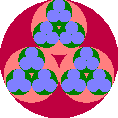
\includegraphics[width=2.0in]{3adicpic.pdf}
\caption*{Figure for Exercise \ref{ex:3adicpic}.}
\end{figure}

Here are some examples of elements of $\Z_5$: 
\small\begin{align*}  (101\bmod{5}, 101\bmod{5^2}, 101\bmod{5^3}, \dots) &=  (1\bmod{5}, 1\bmod{5^2}, 101\bmod{5^3}, \dots),  \\
(-1\bmod{5}, -1\bmod{5^2}, -1\bmod{5^3}, \dots) &= (4\bmod{5}, 24\bmod{5^2}, 124\bmod{5^3}, \dots), \\
(4\bmod{5}, 34\bmod{5^2}, 334\bmod{5^3}, \dots) &= (4\bmod{5}, 9\bmod{5^2}, 84\bmod{5^3}, \dots).
\end{align*}
Take a moment to convince yourself that this last example satisfies our compatibility condition!

\normalsize

\begin{prob}\label{prob:52} $\Z_p$ is a subring of $\prod_{k=1}^{\infty}\Z/p^k$.
\end{prob}

\begin{prob}\label{prob:53} $\Z_p$ is an integral domain.
\end{prob}

\begin{prob}\label{ex:embedding0}\label{prob:54} $\Z_p$ has characteristic $0$. (Thus, $\Z$ sits canonically inside $\Z_p$.)\\
Which elements of $\Q$ can be said to belong to $\Z_p$? Is our third example of a $5$-adic integer an element of $\Q$? (Assume the $n$th component is $3\dots 34\bmod{5^n}$, where $3$ is repeated $n-1$ times.)
\end{prob}

\begin{prob}\label{prob:55} $u = (a_1\bmod{p}, a_2\bmod{p^2}, \dots) \in \Z_p$ is a unit $\Longleftrightarrow$ $p\nmid a_1$ (in $\Z$) $\Longleftrightarrow$ $p\nmid u$ (in $\Z_p$).
\end{prob}


\begin{prob}\label{prob:56} Every nonzero element of $\Z_p$ admits a unique expression in the form $p^v u$, where $v$ is a nonnegative integer and $u$ is a unit in $\Z_p$.
\end{prob}

\begin{prob}\label{prob:57} $\Z_p$ is a principal ideal domain with $p\Z_p$ its only nonzero prime ideal.
\end{prob}

\begin{prob}\label{prob:58}\label{prob:justice} The canonical inclusion $\Z\hookrightarrow \Z_p$ induces an isomorphism $\Z/p^n \cong \Z_p/p^n\Z_p$, for every positive integer $n$.\end{prob}

\begin{prob}\label{prob:59} The definition of $\Z_p$ makes sense without requiring $p$ to be prime. However, considering $\Z_g$ for composite $g$ does not give anything essentially new. In fact: $\Z_{g}\cong \prod_{p\mid g} \Z_p$ for each integer $g>1$. (For instance, $\Z_{10} \cong \Z_2\times \Z_5$.)\index{$\Z_g$, ring of $g$-adic integers!decomposition as $\prod_{p\mid g}\Z_p$}
\end{prob}


\begin{prob}\label{ex:3adicpic}\label{prob:60} What does the picture on this page --- created by \TeX~StackExchange user \texttt{
Qrrbrbirlbel}\footnote{\url{https://tex.stackexchange.com/a/695157}} --- have to do with $\Z_3$?
\end{prob}


\begin{prob}[Steuding]\label{ex:dali} Repeat the last exercise for Salvador Dali's painting \emph{La Cara de la Guerra}.\index{La Cara de la Guerra}
\end{prob}

\begin{prob}[$\Z_p$ is uncountable]\label{prob:61} There is no map from $\Z^{+}$ \underline{onto} $\Z_p$.
\end{prob}

\vspace{-0.1in}
\section*{Well, Color Me Impressed!}
\begin{prob}[Thomas, Monsky]\label{prob:62} Consider the following $3$-coloring of the rational plane $\Q^{2}$: $(x,y)$ is \textsf{red} if $|x|_2 < 1, |y|_2 < 1$, \textsf{blue} if $|x|_2 \ge 1$, $|x|_2 \ge |y|_2$, and \textsf{green} if $|y|
_2 \ge 1$, $|y|_2 > |x|_2$. Show that any trio of differently colored points forms a triangle $\Delta$ with $|\mathrm{Area}(\Delta)|_2 > 1$.

{\scriptsize This observation plays a key role in the proof of \textsf{Monsky's Theorem}\index{Monsky's theorem}: \emph{It is impossible to dissect a square into an odd number of triangles all of which have the same area.}}
\end{prob}

\setcounter{chapter}{6}
\chapter*{$p$-Set \#6}
\addcontentsline{toc}{chapter}{Set \#6}
\markboth{Set \#6}{Set \#6}


\section*{Enter Cauchy}
Let $K$ be a field equipped with an absolute value $|\cdot|$. If $\{x_n\}$ converges to $x$ in $(K,|\cdot|)$, then for any real number $\epsilon > 0$, all terms far enough out in the sequence $\{x_n\}$ are within $\frac{1}{2}\epsilon$ of $x$. By the triangle inequality, all such terms are within $\epsilon$ of each other. That is:
\vskip 0.05in
\fbox{
    \parbox{4.2in}{
        For each $\epsilon > 0$, there is a positive integer $N$ with \[ |x_n - x_m| < \epsilon \quad\text{whenever $n, m \ge N$.}\]
    } (C)
}
\vskip 0.05in
Any sequence $\{x_n\}$ with property (C) is called a \textsf{Cauchy sequence}.\index{Cauchy sequence}

\begin{prob}\label{prob:68} If $|\cdot|$ is non-Archimedean, then $\{x_n\}$ is Cauchy $\Longleftrightarrow$ $|x_{n+1}-x_n| \to 0$. 

{\scriptsize This need not hold if $|\cdot|$ is Archimedean; a counterexample is provided by the partial sums of the harmonic series in $(\Q,|\cdot|_{\infty})$.}
\end{prob}

\begin{prob}\label{prob:70} The sequence $\{2^{5^n}\}$ is Cauchy in $(\Q, |\cdot|_5)$. 
%It does not converge in $(\Q,|\cdot|_5)$ but does converge in $(\Q_5,|\cdot|_5)$, to a $4$th root of $1$.
\end{prob}


\begin{prob}[a common calculus Cauchy claim]\label{prob:68point5} Let $(K,|\cdot|)$ be a valued field. If $\{x_n\}$ is a Cauchy sequence in $K$, then $\{|x_n|\}$ is a bounded sequence of real numbers.
\end{prob}

\begin{prob}[and another] \label{prob:69} Let $(K,|\cdot|)$ be a valued field. If a sequence $\{x_n\}$ of elements of $K$ is Cauchy, and some subsequence of $\{x_n\}$ converges to $x \in K$, then $\{x_n\}$ converges to $x$.
\end{prob}

\vspace{-0.22in}
\testrule 
If $\R$ is equipped with the usual absolute value, then every Cauchy sequence in $\R$ converges to an element of $\R$. This need not be the case for a general valued field. For example, the sequence of rational numbers
\[ x_1 =1, \quad x_2 = 1.4, \quad x_3 = 1.41, \quad x_4 = 1.414,\quad \dots, \]
obtained by successively truncating the decimal expansion of $\sqrt{2}$, is Cauchy in $(\Q,|\cdot|_{\infty})$ but does not converge to any element of $\Q$, since $\sqrt{2}\notin \Q$. Coping with this unsettling scenario was one of the motivations behind the invention (discovery?) of the real numbers in the first place!

Disconcerting examples of this same kind can also be found when $K=\Q$ and $|\cdot| = |\cdot|_p$. Take any sequence $\{c_k\}_{k\ge 0}$ from $\{0,1,\dots,p-1\}$ that is not eventually periodic. Then $x_n = \sum_{k=0}^{n} c_k p^k$ defines a Cauchy sequence in $(\Q,|\cdot|_p)$. To check the Cauchy condition (C), we may assume that $m < n$ (why?). Then  
\[ |x_n - x_m|_p = |c_{m+1} p^{m+1} + c_{m+2} p^{m+2} + \dots + c_n p^{n}|_p < p^{-m},\]
which is smaller than $\epsilon$ once $m > \frac{\log(1/\epsilon)}{\log{p}}$. So (C) is satisfied for any $N > \frac{\log(1/\epsilon)}{\log{p}}$. But $\{x_n\}$ cannot converge to an element of $\Q$, on account of Exercise \ref{ex:rational}.

To get out of this mess, we need to fill in the following blank: $\R$ is to $(\Q,|\cdot|_{\infty})$ as $\underline{\hphantom{nonsense}}$ is to $(\Q,|\cdot|_{p})$. The answer here turns out to be $\Q_p$! But \dots what is $\Q_p$?
\testruletwo

\section*{The $p$-adic Numbers, At Last!}

We define the $\textsf{field of $p$-adic numbers}$\index{p-adic@$p$-adic number|see{$\Q_p$, field of $p$-adic numbers}}, denoted $\Q_p$\index{$\Q_p$, field of $p$-adic numbers!introduction and basic properties},  as the fraction field of  $\Z_p$. Since $\Z_p$ has characteristic $0$, so does $\Q_p$, and thus $\Q\subset \Q_p$.
% As fields of characteristic $0$, each $\Q_p$ contains a canonical copy of $\Q$.

\begin{prob}\label{prob:63} $\Q_p = \bigcup_{n\ge 0} p^{-n} \Z_p =  \Z_p[1/p]$.
\end{prob}

\begin{prob}\label{prob:64} Every nonzero $x \in \Q_p$ admits a unique expression in the form $p^v u$, where $v$ is an integer and $u$ is a unit in $\Z_p$. \end{prob}

For $x \in \Q_p^{\times}$, we set $v_p(x)=v$, where $v$ is the integer from Problem \ref{prob:64}. In order to have $v_p$ defined on all of $\Q_p$, we let $v_p(0)=\infty$. (Compare with the definition of $v_p$ on Set \#1.)

\begin{prob}\label{prob:65} When $x \in \Q$, we have defined $v_p(x)$ twice: once on Set \#1 and again just now, since $x$ is also an element of $\Q_p$. 

Check that when $x \in \Q$ our two definitions of $v_p(x)$ agree (so our sin is venial, rather than mortal). Furthermore, if we set $|x|_p = p^{-v_p(x)}$ for $x \in \Q_p$, then $|\cdot|_p$ defines a non-Archimedean absolute value on $\Q_p$. (We continue to call $v_p$ the \textsf{$p$-adic valuation}\index{p-adic@$p$-adic!valuation} and $|\cdot|_p$ the \textsf{$p$-adic absolute value}.)\index{absolute value!$p$-adic}\index{p-adic@$p$-adic!absolute value}
\end{prob}

\begin{prob}\label{prob:66} $\Z_p = \{x \in \Q_p: |x|_p \le 1\}$. (That is, $\Z_p=\Dd_{\le 1}(0)$ in $\Q_p$.) \\
Also, $\Z_p^{\times} = \{x \in \Q_p: |x|_p = 1\}$.
\end{prob}
\begin{prob}[$\Z_p$ is compact]\index{$\Z_p$, ring of $p$-adic integers!is compact}\label{prob:67}\label{prob:zpcompact} Let $x_1, x_2, x_3, \dots$ be a sequence of elements of $\Z_p$. Infinitely many $x_n$ share the same mod $p$ component, say $a_1\bmod{p}$. Among these, infinitely many share the same mod $p^2$ component, $a_2\bmod{p^2}$. Etc. Thus:      $x_1,x_2,x_3,\dots$ contains a subsequence converging to $(a_1\bmod{p}, a_2\bmod{p^2}, a_3\bmod{p^3}, \dots) \in \Z_p$. 
\end{prob}




\curious

\begin{prob}[Stern]\label{prob:71} Recall that $\log\frac{1}{1-t} = t+\frac{1}{2}t^2 +\frac{1}{3}t^3+  \dots$ whenever $t$ is a complex number with $|t| < 1$ (usual absolute value). Exponentiating, $\e^{T} \e^{T^2/2} \e^{T^3/3} \cdots =\frac{1}{1-T}$, as formal power series. Expanding and comparing coefficients of $T^p$ shows that $|1 - \frac{1}{p!} - \frac{1}{p}|_{p} \le 1$. Hence, $(p-1)!\equiv -1\pmod{p}$ (\textsf{Wilson's theorem}).\index{Wilson's theorem}
\end{prob}


\begin{prob}\label{prob:72} For each prime $p$ and each $a\in \Z$ coprime to $p$, put $q_p(a) = \frac{a^{p-1}-1}{p}$. By Fermat's little theorem, $q_p(a) \in \Z$. 

Prove: If $a$ and $b$ are both coprime to $p$, then $q_p(ab) \equiv q_p(a) + q_p(b) \pmod{p}$.
\end{prob}









\setcounter{chapter}{7}
\chapter*{$p$-Set \#7}
\addcontentsline{toc}{chapter}{Set \#7}
\markboth{Set \#7}{Set \#7}



\section*{You Complete Me}
%\setlength{\epigraphwidth}{0.53\textwidth} 
\epigraph{Why does $\Q$ want to grow to $\R$ or $\Q_2$ or $\Q_3$? Its heart has holes, for example at $\sqrt{2}$ and $\sqrt{3}$. This
is similar to mankind; we can grow to be big boys or big girls, but there is still some sadness in our hearts, and we grow to love another person.\index{sadness in our hearts}}{Kazuya Kato}
% \doubleepigrapha{Why does $\Q$ want to grow to $\R$ or $\Q_2$ or $\Q_3$? Its heart has holes, for example at $\sqrt{2}$ and $\sqrt{3}$. This
% is similar to mankind; we can grow to be big boys or big girls, but there is still some sadness in our hearts, and we grow to love another person.}{Kazuya Kato}{Empty spaces fill me up with holes\\
% Distant limits with no place here to go\\
% Without them within me I fail Cauchy's test\\
% Where I converge is anybody's guess}{Keith Conrad, \emph{Incomplete} (Backstreet Boys song parody)}
\setlength{\epigraphwidth}{0.45\textwidth}  

 
Let $(K,|\cdot|)$ be a valued field. We call $K$ \textsf{complete}\index{completeness of a valued field} if every Cauchy sequence of elements of $K$ converges to an element of $K$. Intuitively, completeness means that ``everything in the world happens for a reason''\footnote{\textsc{Disclaimer}: ``Everything in the world'' means every occurrence of a sequence being Cauchy.}: the far-out terms of a sequence only clump together when they have a compelling justification for doing so, namely heading towards a single value.

\begin{prob}\label{ex:zpcomplete}\label{prob:76} Every Cauchy sequence in $\Z_p$ has a limit belonging to $\Z_p$.
\end{prob}

\begin{prob}\label{ex:qpcomplete}\label{prob:77} Every Cauchy sequence in $\Q_p$ has a limit belonging to $\Q_p$. That is, $\Q_p$ is complete.\index{$\Q_p$, field of $p$-adic numbers!is complete}
\end{prob}

\begin{prob}\label{prob:77andahalf} In $\Q_5$, $\lim 2^{5^n}$ is a $4$th root of $1$. Is $\lim 2^{5^n} \in \Q$?
\end{prob}

\begin{prob}\label{prob:78} $\Z$ is \textsf{dense} in $\Z_p$. In other words, every element of $\Z_p$ is the limit of a sequence of terms from $\Z$.\index{$\Z_p$, ring of $p$-adic integers!has $\Z$ as a dense subset}
\end{prob}

\begin{prob}\label{prob:79} $\Q$ is dense in $\Q_p$.\index{$\Q_p$, field of $p$-adic numbers!has $\Q$ as a dense subset}
\end{prob}

Suppose $K$ and $L$ are fields equipped with absolute values and that the absolute value $|\cdot|$ on $L$ extends the absolute value on $K$. If $(L,|\cdot|)$ is complete and $K$ is a dense subset of $L$, we call $L$ the \textsf{completion of $K$ with respect to $|\cdot|$}.\index{completion of a valued field} For example, $\R$ is the completion of $\Q$ with respect to $|\cdot|_{\infty}$. By Exercises \ref{ex:qpcomplete} and \ref{prob:79}, $\Q_p$ is the completion of $\Q$ with respect to $|\cdot|_p$. 

Why do we say \underline{the} completion and not \underline{a} completion? Completions are unique, up to isometric (absolute-value preserving) isomorphism. 

\begin{prob}\label{prob:80}\index{completion of a valued field!is unique} If $(L,|\cdot|)$ and $(L',|\cdot|')$ are two completions of the same valued field $(K,|\cdot|_0)$, then there is an isomorphism $\phi\colon L \to L'$ that fixes $K$ and satisfies $|\phi(x)|' = |x|$ for all $x \in L$.
\end{prob}


\section*{Hands On, Digits Out}
% %\setlength{\epigraphwidth}{0.58\textwidth}
% \epigraph{Expansion in $\Z_p$ is just like decimal expansion, except that 10 is not prime and the expansion goes the wrong way.}{Hendrik Lenstra}
% %\setlength{\epigraphwidth}{0.45\textwidth}

\begin{prob}\label{prob:81} If $c_0, c_1, c_2, \dots$ is any sequence of integers, then $\sum_{k\ge 0} c_k p^k$ converges to an element of $\Z_p$.
\end{prob}

\vspace{-0.22in}
\testrule
Restricting the ``digits'' $c_k$ in Problem \ref{prob:81} to $\{0,1,2,\dots,p-1\}$, we find that every infinite base $p$ expansion determines an element of $\Z_p$. What about the other way around? Does every element of $\Z_p$ admit an infinite base $p$ expansion? 

Let's suppose that $x\in \Z_p$ can be expanded in base $p$ and see where this leads us. Write $x = c_0 + c_1 p + c_2 p^2 + \dots$, with all $c_i \in \{0,1,\dots,p-1\}$. Then the digit in the $p^k$-place is given by
\[ c_k = \frac{(c_0 + c_1 p + \dots + c_k p^k) - (c_0 + c_1 p + \dots + c_{k-1}p^{k-1})}{p^k}.\]
The parenthesized terms in the numerator are the (least nonnegative integer) reductions of $x$ modulo $p^{k+1}\Z_p$ and modulo $p^k\Z_p$. (Make sure you see why!) So we've determined the digits $c_k$ in any possible expansion of $x$. Now that we know to try these digits, we are home free, as you are asked to check in the next exercise.
\testruletwo

\begin{prob}\label{prob:82}\index{$\Z_p$, ring of $p$-adic integers!base $p$ expansions of elements} Let $x \in \Z_p$, and let $x_k$ ($k=0, 1,2,3,\dots$) be the unique integer in the range $0 \le x_k < p^k$ with $x\equiv x_k\pmod{p^k\Z_p}$. Define
\[ c_k = \frac{x_{k+1}-x_k}{p^k} \quad\text{for $k=0,1,2,\dots$}, \]
Then each $c_k \in \{0,1,2,\dots,p-1\}$, each $x_k = c_0 + c_1 p + \dots  + c_{k-1} p^{k-1}$, and 
\[ x = c_0 + c_1 p + c_2 p^2 + c_3 p^3 + \dots. \] 
{\scriptsize Thus, the (finite) base $p$ expansions of the $x_k$ coalesce to an infinite base $p$ expansion of $x$. The representation produced in this way is not merely \emph{an} infinite base $p$ expansion of $x$, but --- as the lead-in to the problem establishes --- its \emph{unique} base $p$ expansion.}
\end{prob}


% \begin{prob}\label{ex:digitzp}\label{prob:83} The  expansion constructed in Exercise \ref{prob:82} gives the only way to write $x$ as $c_0 + c_1 p + c_2 p^2  \dots$, with each $c_i \in \{0,1,2,\dots,p-1\}$.
% \end{prob}

% \begin{prob} Let $x \in \Z_p$. For each $k=0,1,2,\dots$, let $x_k$ be defined as in Problem \ref{prob:82}. If the familiar base $p$ of expansion of $x_k$ has the form $x_k = c_0 + c_1 p + \dots + c_{k-1} p^{k-1}$, then the canonical expansion of $x$ begins as $x=c_0 + c_1 p + \dots + c_{k-1} p^{k-1} + \dots$. 
% \end{prob}

\begin{prob}[canonical expansions for elements of $\Q_p$]\label{prob:qpdigits}\label{prob:84}\index{$\Q_p$, field of $p$-adic numbers!base $p$ expansions of elements}\index{canonical expansions of elements of $\Q_p$} For each $x \in \Q_p$, there is a unique two-sided sequence of integers $\{c_k\}_{k=-\infty}^{\infty}$ satisfying
\begin{enumerate}
    \item[(i)] each $c_k \in \{0,1,2,\dots,p-1\}$,
    \item[(ii)] $c_k$ is nonzero for only finitely many $k < 0$,
    \item[(iii)] $x = \sum_{k} c_k p^k$.
\end{enumerate}
\end{prob}


\begin{prob}\label{prob:85} The canonical expansion of $x \in \Q_p$ 
%from Problem \ref{prob:qpdigits}
terminates (meaning that $c_k=0$ for all large enough $k$) $\Longleftrightarrow$ $x=0$ or $x\in\Q^{+}$ with denominator a power of $p$.
\end{prob}

\begin{prob}\label{prob:86} The canonical expansion of $x\in \Q_p$ is eventually periodic $\Longleftrightarrow$ $x\in\Q$.\index{$\Q_p$, field of $p$-adic numbers!element has eventually periodic base $p$ expansion iff rational}
\end{prob}

\vspace{-0.1in}
\curious

\begin{prob}\label{ex:wilson00}\label{prob:87}  For every odd prime $p$:\quad $\displaystyle\sum_{a=1}^{p-1} \frac{a^{p-1}-1}{p} \equiv \frac{(p-1)! + 1}{p} \pmod{p}$. 
\end{prob}


\section*{Method of Successive Approximation}

\begin{prob}[computing a value of $\sqrt{2}$ in $\Z_7$]\index{method of successive approximation} \label{ex:hensel0}\label{prob:98} We can compute a square root of $2$ in $\Z_7$ by determining a root in $\Z/7$, then $\Z/7^2$, then $\Z/7^3$, $\dots$, being mindful to maintain compatibility throughout the process.

To start things off, the residue class $x_1 = 3\bmod{7}$ satisfies $x^2 = 2$ in $\Z/7$. This solution can be lifted, uniquely, to a solution of $x^2=2$ in $\Z/7^2$. To see why, note that a generic integer congruent to $3\pmod{7}$ has the form $3+7k$, and 
$(3+7k)^2 = 9 + 42k + 7^2 k^2\equiv 9 + 42k\pmod{7^2}$. The congruence $9+42k\equiv 2\pmod{7^2}$ is satisfied precisely when $k\equiv 1\pmod{7}$. For integers $k\equiv 1\pmod{7}$, we have $3+7k\equiv 10\pmod{7^2}$. Therefore, $x_2:=10\bmod{7^2} \in \Z/7^2$ is the lift we are after.

Expanding $(10+7^2 k)^2$ mod $7^3$, and reasoning analogously, will show that $x_2=10\bmod{7^2}$ lifts uniquely to $x_3:=10+7^2\cdot 2 = 108\bmod{7^3}$. 

This process can be continued indefinitely, uniquely determining $x_1, x_2, x_3, \dots$. 
Then $x:=(x_1, x_2, x_3,\dots) \in \prod_{k=1}^{\infty} \Z/7^k$ is a solution in $\Z_7$ to $x^2=2$. The canonical base $7$ expansion of $x$ begins
\[  3 + 1\cdot 7 + 2\cdot 7^2 + 6\cdot 7^3 + \dots.\]

{\scriptsize After that wall of text, you might be wondering what exactly you are being asked to do. Your job: Check that the process can be continued indefinitely, uniquely determining all the $x_k$, that setting $x = (x_1, x_2, x_3, \dots)$ really does define a $\Z_7$-solution to $x^2=2$, and finally, that the $7$-adic expansion of $x$ starts the way we claimed.}
\end{prob}



% \begin{prob} Every $x\in\Z_p$ admits a unique expansion $c_0 + c_1(-p) + c_2 p^2 + c_3(-p)^3 + c_4 p^4 + \dots$, with each $c_i \in \{0,1,\dots,p-1\}$. This expansion terminates precisely when $x \in \Z$.    
% \end{prob}














\setcounter{chapter}{8}
\chapter*{$p$-Set \#8}
\addcontentsline{toc}{chapter}{Set \#8}
\markboth{Set \#8}{Set \#8}


\section*{The World (of $p$-adic) Series}

% \epigraph{With the exception of the very simplest cases \dots there are almost no infinite series in mathematics whose sum has been rigorously determined.}{Niels Henrik Abel}

\begin{prob}\label{ex:seriesconvergence}\label{prob:89} Let $K$ be a field complete with respect to a non-Archimedean absolute value $|\cdot|$ (for instance, $\Q_p$!). 
\begin{enumerate}\vspace{-0.05in}
    \item[(a)] A series $\sum_{k=1}^{\infty} a_k$ converges in $K$ $\Longleftrightarrow$ $a_k \to 0$ in $K$. 
    \item[(b)] If $\sum_{k=1}^{\infty} a_k$ converges, then $\left|\sum_{k=1}^{\infty} a_k\right| \le \max_{k=1,2,3,\dots} |a_k|$.
\end{enumerate}
\index{convergence of infinite series}\index{$\Q_p$, field of $p$-adic numbers!convergence of series}\index{strong triangle inequality!extension to infinite series in $\Q_p$}
\end{prob}

For the next exercise, recall that a \textsf{rearrangement} of a series $\sum_{k=1}^{\infty} a_k$ is a series of the form $\sum_{k=1}^{\infty} a_{\sigma(k)}$, where $\sigma$ is a permutation of $\Z^{+}$ (a bijection of $\Z^{+}$ with itself).

\begin{prob}\label{prob:90} Let $K$ be a field complete with respect to a non-Archimedean absolute value. If $\sum_{k=1}^{\infty} a_k$ is a series in $K$ that converges to $s\in K$, then every rearrangement of $\sum_{k=1}^{\infty} a_k$ also converges to $s$.
\end{prob}


\begin{prob}\label{prob:93} Suppose that $\sum_{n=0}^{\infty} a_n$ and $\sum_{n=0}^{\infty} b_n$ are convergent series in the field $K$, which is assumed complete with respect to a non-Archimedean absolute value. Define $c_n = \sum_{k=0}^{n} a_k b_{n-k}$, for $n=0,1,2,\dots$. Then $\sum_{n=0}^{\infty} c_n$ converges and in fact $\sum_{n=0}^{\infty} c_n = (\sum_{n=0}^{\infty} a_n) (\sum_{n=0}^{\infty} b_n)$.

{\scriptsize \underline{Important consequence}: If $F(T) = \sum_{k=0}^{\infty} a_k T^k$,  $G(T) = \sum_{k=0}^{\infty} b_k T^k \in K[[T]]$ both converge at the point $z \in K$, so does $F(T)G(T)$, and $F(T)G(T)|_{T=z} = F(z) G(z)$. }
\end{prob}





\begin{prob}[a doubleheader?]\label{ex:doubleseries}\label{prob:91} Let $K$ be a field complete with respect to a non-Archimedean absolute value $|\cdot|$. Let $\{a_{i,j}\}_{i,j\ge 0}$ be a doubly-indexed sequence of elements of $K$. Suppose there is a sequence of real numbers $\{\epsilon_N\}_{N\ge 0}$ tending to $0$ with the property that 
\[ |a_{i,j}|_p \le \epsilon_N \quad\text{whenever $i\ge N$ or $j\ge N$}.\footnote{This may seem a strange condition to impose on $\{a_{i,j}\}$. In fact, it's very natural; it's equivalent to asking that for each $\epsilon > 0$, the inequality $|a_{i,j}| < \epsilon$ fails at most finitely often. We could have phrased the requirement this way to start with, but our more elaborate formulation will turn out to be easier to work with in proofs.} \]        
Show: The double series $\sum_{i}  \sum_{j} a_{i,j}$ and $\sum_{j}\sum_{i} a_{i,j}$ both converge.
\end{prob}

\begin{prob}[a double switch]\label{prob:92} Continue with the notation and assumptions of Exercise \ref{ex:doubleseries}. For every nonnegative integer $N$,
\[  \left|\sum_{i} \sum_{j} a_{i,j} - \sum_{i=0}^{N} \sum_{j} a_{i,j}\right| \le \epsilon_{N+1}, \quad \left|\sum_{j} \sum_{i} a_{i,j} - \sum_{j} \sum_{i=0}^{N} a_{i,j}\right| \le \epsilon_{N+1},\]
\[ \left|\sum_{i=0}^N \sum_{j} a_{i,j} - \sum_{i=0}^{N} \sum_{j=0}^{N} a_{i,j}\right| \le \epsilon_{N+1}, \quad \left|\sum_{j} \sum_{i=0}^{N} a_{i,j} - \sum_{j=0}^{N} \sum_{i=0}^{N} a_{i,j}\right| \le \epsilon_{N+1}.\]
Therefore, $\sum_{i}\sum_{j} a_{i,j} = \sum_{j}\sum_{i} a_{i,j}$.\end{prob}


\section*{Are You Feeling the Bern?}

Recall from Set \#4 that when $k,n\in \Z^{+}$, we are writing $S_k(n) =1^k + 2^k + \dots + (n-1)^k$. 
%In the next series of exercises, $p$ denotes a prime (as usual). 

% \begin{prob}\label{ex:vsc0} $S_k(p) \equiv \begin{cases}
% -1\pmod{p}&\text{if $p-1\mid k$},\\
% 0\pmod{p}&\text{otherwise}.
% \end{cases}$quad
% \end{prob}

\begin{prob}\label{prob:newbern0} For $p$ prime, $k\in \Z^{+}$:\quad $p\mid (S_k(p) + \mathbf{1}_{p-1\mid k})$.
\end{prob}
{\scriptsize $\one_{C}$\index{$1$@$\one_C$, indicator function of $C$} denotes the indicator function of the condition $C$. Thus, $\one_{p-1\mid k}$ is $1$ if $p-1$ divides $k$ and $0$ otherwise.}

\begin{prob}\label{prob:newbern1} For $p$ prime, $k\in \Z^{+}$:\quad $B_k + \frac{\mathbf{1}_{p-1\mid k}}{p} + \sum_{0 < j < k} \binom{k}{j} B_{k-j} \frac{p^j}{j+1} \in \Z_{(p)}$.
\end{prob}

\begin{prob}\label{prob:newbern2} For $p$ an odd prime, $k\in \Z^{+}$:\quad  $B_k + \frac{\mathbf{1}_{p-1\mid k}}{p} \in \Z_{(p)}$.
\end{prob}

\begin{prob}\label{prob:newbern3} For $k\in 2\Z^{+}$:\quad $B_{k} + \frac{1}{2} \in \Z_{(2)}$.
\end{prob}





% \begin{prob}\label{ex:vsc0}\label{prob:94} In $(\Q, |\cdot|_p)$:\quad $\lim_{s\to\infty} S_k(p^s) p^{-s} = B_k$.
% \end{prob}

% \begin{prob}\label{prob:95} Let $k \in \Z^{+}$. For $s \in \Z^{+}$, let $I_j = [j\cdot p^{s}, (j+1)p^s)$ for $j=0,\dots,p-1$. For each $j$,
% \[ \sum_{n \in I_j} n^k \equiv S_k(p^s) + kj p^s S_{k-1}(p^s) \pmod{p^{s+1}}.\] 
% \end{prob}

% \begin{prob}\label{prob:96} For $k\in 2\Z^{+}$, $s\in \Z^{+}$:\quad $S_k(p^{s+1}) \equiv p S_k(p^s)\pmod{p^{s+1}}$. Therefore,
% \[ \frac{S_k(p^{s+1})}{p^{s+1}}-\frac{S_k(p^s)}{p^s} \in \Z_{(p)}. \]
% \end{prob}

\begin{prob}[Clausen, von Staudt]\label{ex:vsclast}\label{prob:97} For $k \in 2\Z^{+}$:\quad
% If $k\in 2\Z^{+}$, then $B_k \in \Z_{(p)}$ unless $p-1\mid k$, in which case $B_k + \frac{1}{p} \in \Z_{(p)}$. As a consequence
$\displaystyle B_k + \sum_{\substack{p\text{ prime } \\ p-1 \mid k}} \frac{1}{p} \in \Z$.\index{Bernoulli numbers!Clausen--von Staudt theorem}\index{Clausen--von Staudt theorem}

{\scriptsize It follows from Exercise \ref{ex:vsclast} that the denominator of $B_k$ is the (squarefree!) product of the primes $p$ for which $p-1\mid k$.}
\end{prob}

\section*{Finding Your Roots}

\begin{prob}[Teichm\"{u}ller representatives]\label{prob:teichmuller}\index{Teichm\"{u}ller representatives}\index{respectable mathematician!non-example, \emph{see bottom of}} For each $u \in \Z_p^{\times}$, the field $\Q_p$ contains a unique $(p-1)$th root of unity congruent to $u\bmod{p\Z_p}$, namely $\omega(u):= \lim_{n\to\infty} u^{p^n}$.\index{$\omega(u)$|see{Teichm\"{u}ller representatives}}
\end{prob}

\begin{prob}\label{prob:teichmullercalculation} Find $\omega(2)$ (exactly) when $p=3$. Then take $p=7$ and determine the digits $c_0, c_1, c_2$ in the canonical expansion $\omega(2) =  c_0 + c_1 \cdot 7 + c_2 \cdot 7^2 + \dots$.
\end{prob}

\begin{prob}\label{prob:WJteich} If $u\in \Z$ has order $3$ modulo $p$, then $1+u$ has order $6$ mod $p$, and $\omega(1+u)=1+\omega(u)$.
\end{prob}




% \begin{prob} Interpret $2^{2^{2^{\iddots}}}$ as an element of $\Z_3$. Can you do this in $\Z_5$? in $\Z_p$?
% \end{prob}
 

\setcounter{chapter}{9}
\chapter*{$p$-Set \#9}
\addcontentsline{toc}{chapter}{Set \#9}
\markboth{Set \#9}{Set \#9}


\setlength{\epigraphwidth}{0.45\textwidth}
\epigraph{Is $\R$ special? Well, physical reality, as we and Archimedes believe it, has no infinitesimals\dots. Hence we say that the field $\R$ and its
absolute value $|\cdot|_{\infty}$ are \emph{archimedean}\dots. 
\emph{pace} Archimedes, in recent years the theoretical physicists have learned about the $p$-adic fields and
have begun to wonder whether they may not help in modeling just what
happens in the nuclei of atoms, for instance. So much for reality.}{Alf van der Poorten}
\setlength{\epigraphwidth}{0.45\textwidth}


\section*{Gazing at the Newfound Stars}
\begin{prob}\label{prob:99} Let $p$ be odd. Let $a \in \Z_p^{\times}$, and let $a_1 \bmod{p}$ be the mod $p$ component of $a$. Then $a \text{ is a square in $\Q_p$} \Longleftrightarrow a_1\bmod{p} \text{ is a square in $\Z/p$}$. 

{\scriptsize Suggestion. Adapt the method of successive approximation\index{method of successive approximation} described in Exercise \ref{ex:hensel0}.}
\end{prob}

\begin{prob}\label{prob:100} Let $p$ be odd, and let $n \in \Z$ be a nonsquare mod $p$. Then $1,  n$ are coset representatives for $\Z_p^{\times}/(\Z_p^{\times})^2$, while $1, n, p, np$ are coset representatives for $\Q_p^{\times}/(\Q_p^{\times})^2$.\index{$\Z_p$, ring of $p$-adic integers!structure of $\Z_p^{\times}/(\Z_p^{\times})^2$}\index{$\Q_p$, field of $p$-adic numbers!structure of $\Q_p^{\times}/(\Q_p^{\times})^2$}  
\end{prob}

\begin{prob}\label{prob:101} If $a\in \Z_2^{\times}$, then $a$ is a square in $\Q_2$ $\Longleftrightarrow$ $a\equiv 1\pmod{8\Z_2}$.
\end{prob}


\begin{prob}\label{prob:102} Find coset representatives for $\Z_2^{\times}/(\Z_2^{\times})^2$ and $\Q_2^{\times}/(\Q_2^{\times})^2$. 
\end{prob}

\begin{prob}\label{prob:103}
For $a \in \Q_p^{\times}$: 
\[ a \in \Z_p^{\times} \Longleftrightarrow \text{(some value of) $\sqrt[n]{a} \in \Q_p$ for infinitely many $n\in \Z^{+}$}. \]
\end{prob}


\begin{prob}[a Liouville approximation theorem in $\Z_p$]\index{Liouville's approximation theorem in $\Z_p$}\label{prob:104} Suppose $\alpha \in \Z_p$ is a root of a polynomial $F(T) \in \Z[T]$ of degree $d$ having no integer roots. For every nonzero $n \in \Z$,
\[ |n-\alpha|_{p} \ge |F(n)-F(\alpha)|_{p} = |F(n)|_p \ge |F(n)|_{\infty}^{-1} \ge c|n|_{\infty}^{-d}, \]
where $c$ is a positive constant depending only on $F$.
\end{prob}




\begin{prob}[a transcendental element of $\Q_p$]\label{prob:105} $\sum_{k\ge 1} p^{k!}\in \Q_p$ is not a root of any nonconstant polynomial in $\Q[x]$.\end{prob}


\begin{prob}\label{prob:106} $2^{4\cdot 5^n}\to 1$ in $\Z_{5}$ while $2^{4\cdot 5^n}\to 0$ in $\Z_{2}$. Since $0$ and $1$ are distinct rational numbers, the $\Z_{10}$-limit of $2^{4\cdot 5^n}$ has a nonperiodic $10$-adic expansion.\index{$\Z_g$, ring of $g$-adic integers!example of $\Z_{10}$} 

{\scriptsize Since $10$ is not prime, your solution should start with a sensible definition of convergence in $\Z_{10}$.}

\end{prob} 


\section*{Strassmann Series}
Let $F(T) = \sum_{n \ge 0} a_n T^n$ be a formal power series with $\Q_p$-coefficients.

\begin{prob}\label{prob:strass0}\label{prob:107} For $x \in \Q_p$:~\,$F(x)$ converges $\Longleftrightarrow$ $|a_n x^n|_p\to 0$.\\ Hence, $F(x)$ converges for all $x \in \Z_p$ $\Longleftrightarrow$ $a_n\to 0$ in $\Q_p$.
\end{prob}

\vspace{-0.05in}When $F(x)$ converges for all $x \in \Z_p$, we call $F(T)$ a \textsf{Strassmann (power) series}.\index{Strassmann series!definition}\index{restricted power series|see{Strassmann series}}\index{strictly convergent power series|see{Strassmann series}}\footnote{Here we depart from convention; the usual terms are \textsf{restricted power series} or \textsf{strictly convergent power series}.}

\vspace{-0.22in}
\testrule
In courses on complex function theory, one learns that an analytic function has only finitely many zeros in a closed disc, unless it vanishes identically on that disc. The next three exercises guide you through a proof of an analogous result for zeros of Strassmann series within $\Z_p$.
\testruletwo

\begin{prob}\label{prob:108} Let $F(T)$ be a Strassmann series with a nonzero coefficient. Any nonzero $x \in \Z_p$ with $F(x) = 0$ satisfies $|x|_p \ge \delta$, where $\delta > 0$ is a constant depending only on $F$. If $F(T)$ has $\Z_p$-coefficients, we can take $\delta = |a_m|_p$, where $a_m$ is the first nonvanishing coefficient of $F(T)$. 

In particular: If $F(T)$ is a Strassmann series and $F(x) = 0$ for all $x \in \Z_p$, then $F(T) = 0$ in $\Q_p[[T]]$.
\end{prob}

\begin{prob}[recentering Strassmann series]\label{prob:109} Let $F(T)= \sum_{k \ge 0} a_k T^k$ be a Strassmann power series, and let $x_0 \in \Z_p$. For every $x \in \Z_p$,
\[ F(x+x_0) = \sum_{j\ge 0} b_j x^j, \quad\text{where}\quad b_j:= \sum_{k \ge j} a_k \binom{k}{j} x_0^{k-j}. \]
The recentered series $\sum_{j \ge 0} b_j T^j$ is also Strassmann.
\end{prob}

\begin{prob}\label{ex:weakstrass}\label{prob:110} A Strassmann series with a nonvanishing coefficient has finitely many zeros in $\Z_p$.\index{Strassmann series!if nonzero has finitely many zeros in $\Z_p$}
\end{prob}


\curious

 


\begin{prob}[Glaisher]\label{ex:wilson1}\label{prob:111}\index{Bernoulli numbers!associated characterization of Wilson primes} For all primes $p$:\quad $p^2 \mid (p-1)! + 1 \Longleftrightarrow B_{p-1} + \frac{1}{p}-1 \in p\Z_{(p)}$.

{\scriptsize Primes $p$ for which $p^2\mid (p-1)!+1$ are known as Wilson primes.\index{Wilson prime} The only known examples, and the only examples smaller than $2\cdot 10^{13}$, are $5$, $13$, and $563$.}
\end{prob}  

\begin{prob}[Johnson]\label{prob:WJfermat}\index{Teichm\"{u}ller representatives} Recall that when $u\in \Z_p^{\times}$, we are writing $\omega(u)$ for the unique $(p-1)$th root of unity congruent to $u$ modulo $p\Z_p$ (see Exercise \ref{prob:teichmuller}). Show that if $u\in \Z$ has order $3$ modulo $p$, and $v\in \Z$ satisfies $v\equiv \omega(u) \pmod{p^k\Z_p}$, where $k\in \Z^{+}$, then
\[ (1+v)^p \equiv 1+v^p \pmod{p^{2k+1}}. \]
Use this to explain the congruence $325^7 \equiv 1 + 324^7 \pmod{7^7}$.
\end{prob}


{\setlength{\tabcolsep}{16pt}
\begin{table}[b]
    \centering
        
    \label{tab:my_label}
    \begin{tabular}{rr}\toprule

    \multicolumn{1}{r}{$u$} & \multicolumn{1}{r}{$\omega(u)$}\\ \cmidrule(lr){1-1}\cmidrule(lr){2-2}          2&  $2 + 4\cdot7 + 6\cdot7^2 + 3\cdot7^3 + 2\cdot7^5+\dots$\\
          3&  $3 + 4\cdot7 + 6\cdot7^2 + 3\cdot7^3 + 2\cdot7^5+\dots$ \\
          4& $4 + 2\cdot7 + 3\cdot7^3 + 6\cdot7^4 + 4\cdot7^5+\dots$\\
          5& $5 + 2\cdot7 + 3\cdot7^3 + 6\cdot7^4 + 4\cdot7^5+\dots$\\\bottomrule
        
    \end{tabular}
\caption*{Sixth roots of unity in $\Q_7$, omitting $\omega(\pm 1)=\pm 1$. Notice that $\omega(3)=1+\omega(2)$ and $\omega(5) = 1+\omega(4)$, as guaranteed by Problem \ref{prob:WJteich}.\index{Teichm\"{u}ller representatives}}
\end{table}}

\setcounter{chapter}{10}
\chapter*{$p$-Set \#10}
\addcontentsline{toc}{chapter}{Set \#10}
\markboth{Set \#10}{Set \#10}

\setlength{\epigraphwidth}{2.35in}
\renewcommand{\epigraphflush}{flushright}
\epigraph{If you claim a series sums to $S$\\
Your metric you must not suppress\\
The danger, you can now see \\
Is that another may disagree \\
And you may both be right: what a mess!}{Edward B. Burger\\ Thomas Struppeck}

\section*{I \dots Have \dots the \dots Power\dots (Series)}
One can often leverage identities from the real universe to establish corresponding results in the $p$-adic realm. As a proof of concept, consider the following formula you may have encountered in your study of Taylor series: For all real numbers $x$ with $|x| < 1$, 
\begin{align*} \sqrt{1+x} &= 1 +\frac12 x -\frac18 x^2 + \frac1{16} x^3 - \frac{5}{128}x^4+\dots
\\ 
&=\sum_{k\ge 0} \binom{\frac12}{k} x^k, \qquad\text{where}\quad\binom{\frac12}{k} := \frac{\frac{1}{2}(\frac{1}{2}-1)\cdots(\frac{1}{2}-(k-1))}{k!}. \end{align*}
We will argue that the same sum on $k$ defines a square root of $1+x$ in $\Q_p$ whenever it converges.

Getting from $\R$ to $\Q_p$ requires a stopover in the land of formal power series. Let $B_{\frac12}(T) = \sum_{k\ge 0} \binom{\frac12}{k} T^k \in \Q[[T]]$, and let $C(T) = B_{\frac 12}(T)^2$, the formal square of $B_{\frac{1}{2}}(T)$. We claim that $C(T)=1+T$.

To fashion a proof, suppose $x$ is a real number with $|x|<1$. Then $B_{\frac12}(x)$ converges absolutely (e.g., by the ratio test). So if we multiply $B_{\frac12}(x)$ by $B_{\frac12}(x)$, we can reshuffle the terms as we please. One such regrouping gives us $C(x)$. On the other hand, our ``real world'' identity says that $B_{\frac12}(x)^2 = 1+x$ whenever $|x| < 1$. It follows that $C(x) - (1+x)=0$ when $|x| < 1$. But a power series that vanishes on an open interval around $0$ has all its coefficients equal to $0$. This forces $C(T) = 1+T$, as formal series.

Armed with this formal identity, we can head back to $\Q_p$. Suppose we have in hand an $x\in \Q_p$ for which $B_{\frac12}(x)$ converges. If we multiply $B_{\frac12}(x)$ by $B_{\frac12}(x)$, we can rearrange the result into $C(x)$ --- this time justifying ourselves not on the basis of absolute convergence but by an appeal to Problem \ref{prob:93}. Since $C(x)=1+x$, this shows that $B_{\frac{1}{2}}(x)$ represents a square root of $1+x$ in $\Q_p$ whenever $B_{\frac{1}{2}}(x)$ converges.

\begin{prob}\label{prob:F12convergence} If $p$ is odd, then $B_{\frac12}(x)$ converges when $|x|_p \le 1/p$. If $p=2$, then $B_{\frac12}(x)$ converges when $|x|_2 \le 1/2^3$. Are these conditions necessary for convergence?
\end{prob}

\begin{prob}\label{prob:differentroots} $B_{\frac12}(\frac{9}{16}) = \sum_{k\ge 0} \binom{\frac12}{k} (\frac{9}{16})^{k}$ converges to $\frac54$ in $\R$ but to $-\frac54$ in $\Q_3$.\end{prob}



%\vspace{-0.1in}





\section*{Lifting and Embedding}

\begin{prob}[Taylor's Formula]\label{prob:113} If $F(T) \in \Q_p[T]$, and $a \in \Q_p$, then 
\[ F(a+T) = \sum_{j\ge 0} \frac{F^{(j)}{(a)}}{j!} T^j. \]
Furthermore: If $F(T) \in \Z_p[T]$, so is $\frac{1}{j!} F^{(j)}(T)$, for all nonnegative integers $j$.\index{Taylor's formula}
\end{prob}

\begin{prob}[$p$-adic Newton's method]\label{prob:114}\index{Newton's method} Let $F(T) \in \Z_p[T]$.  If $x \in \Z_p$ and $|F'(x)|_p=1$, then $\tilde{x} := x- \frac{F(x)}{F'(x)}$ satisfies $|F(\tilde{x})|_p \le |F(x)|_p^2$.
% \equiv 0\pmod{p\Z_p}$ and $F'(x_1)\not\equiv 0\pmod{p\Z_p}$. We can inductively define a sequence of elements of $\Z_p$ by setting
% \[ x_{n+1} = x_n - \frac{F(x_n)}{F'(x_n)},\quad n=1,2,3,\dots. \]
% Each $x_{n+1}\equiv x_n\pmod{p^{2^{n-1}}\Z_p}$ and each $F(x_n)\equiv 0 \pmod{p^{2^{n-1}}\Z_p}$.  
\end{prob}
 

\begin{prob}[Hensel's Lemma]\label{prob:115}\index{Hensel's lemma} Let $F(T) \in \Z_p[T]$. Suppose $x_1 \in \Z_p$ satisfies $F(x_1) \equiv 0\pmod{p\Z_p}$ and $F'(x_1)\not\equiv 0\pmod{p\Z_p}$. Then $F$ has a zero $x\in \Z_p$ satisfying $x\equiv x_1\pmod{p\Z_p}$.
\end{prob}


\begin{prob}\label{prob:116} Suppose $F(T) \in \Z[T]$ is nonconstant with all complex roots distinct. Then $F(T) \Q[T] + F'(T) \Q[T] = \Q[T]$. Hence, $F(T)\Z[T] + F'(T) \Z[T]$ contains a nonzero integer $R$.  Deduce: $F(T)$ and $F'(T)$ are coprime over $\Z/p$ for all but finitely many $p$.
\end{prob}

\begin{prob}\label{prob:117} Every nonconstant $F(T) \in \Z[T]$ has a root in $\Z_p$ for infinitely many primes $p$.
\end{prob}

\begin{prob}\label{ex:embedding}\label{prob:118} Let $K$ be a number field (a finite extension of $\Q$). By the primitive element theorem, $K = \Q(\theta)$ for some $\theta\in K$. Choose $F(T) \in \Z[T]$ irreducible over $\Q$ and vanishing at $\theta$. Then $K$ embeds into $\Q_p$ whenever $F(T)$ has a root in $\Q_p$. Deduce: There is an embedding $K \hookrightarrow \Q_p$ for infinitely many $p$.
\end{prob}


\section*{Don't Ever Change}
\begin{prob}\label{prob:onlyhomomorphism} The only ring homomorphism from $\Q_p$ to $\Q_p$ is the identity.
\end{prob}

\begin{prob}\label{prob:nohomomorphism} There is no ring homomorphism from $\Q_p$ to $\Q_q$ ($q$ prime, $q\ne p$) or to $\R$.
% \footnote{``\dots no manner of squinting seems to be able to make $\R$ the least bit mistakable for any
% of the $p$-adic fields, nor are the $p$-adic fields $\Q_p$ isomorphic for distinct $p$. A major
% theme in the development of Number Theory has been to try to bring $\R$ somewhat more into line with the $p$-adic fields; a major mystery is why $\R$ resists this attempt
% so strenuously.'' --- Barry Mazur}
\end{prob}

{\scriptsize There \emph{is} a field embedding of $\Q_p$ into $\C$ (assuming the Axiom of Choice). In fact, there are many such embeddings, but none are canonical, and none carry convergent sequences in $\Q_p$ to convergent sequences in $\C$. Thus (channeling Hermann Weyl\footnote{Weyl famously wrote ``The introduction of numbers as coordinates \dots\,is an act of violence.''}), choosing such an embedding must always be regarded as something of a brute act.}

\section*{Is Sticking Together Irrational?}
\begin{prob}[Mahler]\label{prob:mahlerirrational} The real number $0.248163264128\dots$ obtained by concatenating the decimal digits of powers of $2$ is irrational.
\end{prob}


\setcounter{chapter}{11}
\setcounter{chapter}{11}
\chapter*{$p$-Set \#11}
\addcontentsline{toc}{chapter}{Set \#11}
\markboth{Set \#11}{Set \#11}
\label{chap:skolem}

\vspace{-0.4in}
%\setlength{\epigraphwidth}{0.51\textwidth}
% \epigraph{Ordinary analysis has amassed a great stock of identities between power series. Many of these are valid in $p$-adic analysis too. But here an identity between power series yields congruences between partial sums.}{Max Zorn}
%\setlength{\epigraphwidth}{0.49\textwidth}
\epigraph{In 1926, when he was nearly 40 years old, Skolem obtained his
doctorate\dots The somewhat advanced age
has the following explanation. In their younger years, Viggo Brun and
Skolem agreed that neither of them would bother to obtain the degree of
Doctor, probably feeling that, in Norway, it served no useful function
in the education of a young scientist. But in the middle twenties a
younger generation of Norwegian mathematician emerged. It seems
that Skolem then felt he too ought to fulfil the formal requirement
of having a doctorate, and he ``obtained permission'' from Brun to
submit a thesis.}{Jens Erik Fenstad}

\vspace{0.12in}
\section*{I \dots Have \dots the \dots Power\dots (Series)}
\begin{prob}[$p$-adic lumber theory]\label{prob:padiclumber1}\index{p-adic@$p$-adic logarithm!definition and convergence on $1+p\Z_p$}\index{logarithm, on $\Q_p$|see{$p$-adic logarithm}} Recall from calculus that \[ \log{x} = \log(1+(x-1)) = \sum_{k\ge 1} \frac{(-1)^{k-1}}{k} (x-1)^k \quad\text{whenever} \quad |x-1| < 1.\] This motivates us to define, for each prime $p$,
\[ \log_p(T) = \sum_{k\ge 1} \frac{(-1)^{k-1}}{k} (T-1)^{k} \in \Q_p[[T-1]]. \] Show: $\log_p{x}$ converges for all $x \in \Q_p$ with $|x-1|_p < 1$.
\end{prob}

\testrule
Passing the familiar identity $\log{xy} = \log{x} +\log{y}$ (valid for $x,y \in \R^{+}$) from $\R$ to $\Q_p[[X-1,Y-1]]$, and then on to $\Q_p$, one can show that
\begin{equation}\tag{$\dagger$} \log_p{x} + \log_p{y} = \log_p(xy) \quad\text{whenever $x,y \in 1 +p\Z_p$}.\end{equation}
Filling in the details here is a bit finicky. If you enjoy this kind of work (you know who you are\dots), give it a try!
\testruletwo

\begin{prob}\label{prob:padiclumber2} Go ahead and assume (\textdagger).

Show: $\displaystyle\sum_{k=1}^{\infty}\left(1+\frac{1}{2^k} + \frac{1}{3^k} + \dots + \frac{1}{(p-1)^k}\right) \frac{p^k}{k}=0$ in $\Q_p$. \\
In particular ($p=2$):\quad $\displaystyle\sum_{k=1}^{\infty}\frac{2^k}{k}=0$ in $\Q_2$.\footnote{``Ordinary analysis has amassed a great stock of identities between power series. Many of these are valid in $p$-adic analysis too. But here an identity between power series yields congruences between partial sums.'' --- Max Zorn}



% {\scriptsize Put $\Exp_p(T)=\sum_{k\ge 0} \frac{T^k}{k!}$. Suppose $p$ is odd (the situation is slightly more complicated when $p=2$). Then $\Exp_p(T)$ converges for $x\in p\Z_p$, and for these same $x$ one has $\Exp_p(\log_p(1+x)) = 1+x$ and $\log_p(\Exp_p(x)) = x$. Also, $\Exp_p(x+y)=\Exp_p(x)\cdot \Exp_p(y)$ for all $x,y\in p\Z_p$.}
\end{prob}



\begin{prob}[derive responsibly!]\label{prob:fakeproofkoblitz} Critique the following proof that $\pi$ is irrational: Suppose that $\pi = \frac{a}{b}$, where $a$ and $b$ are positive integers. Let $p$ be an odd prime not dividing $a$. Then $$0 = \sin(pb \pi) = \sin(ap) = \sum_{k\ge 0} (-1)^k \frac{(ap)^{2k+1}}{(2k+1)!}, $$ 
where this last series converges in $\Q_p$. Therefore,
\[ p^{-1} = |-ap|_p = \left|\sum_{k\ge 0} (-1)^k \frac{(ap)^{2k+1}}{(2k+1)!} -ap\right|_p = \left|\sum_{k\ge 1} (-1)^k \frac{(ap)^{2k+1}}{(2k+1)!}\right|_p\le p^{-2}. \]
Contradiction! \label{ex:pi}
\end{prob}




% \begin{prob} In courses on rigorous calculus, it is shown that when $x$ is  real  with $|x| < 1$, the series $\sum_{k\ge 0} \frac{\frac{1}{2}(\frac{1}{2}-1)\cdots (\frac{1}{2}-(k-1))}{k!} x^k$ converges to the positive square root of  $1+x$. Show that for $p$ odd and $x \in p\Z_p$, that same series converges to the square root of $1+x$ belonging to $1+p\Z_p$. Hence, $\sum_{k\ge 0} \frac{\frac{1}{2}(\frac{1}{2}-1)\cdots (\frac{1}{2}-(k-1))}{k!} (9/16)^{k}$ converges to $5/4$ in $(\R,|\cdot|)$ but to $-5/4$ in $(\Q_3,|\cdot|_3)$.
% \end{prob}

\section*{Strassmann Series}

\begin{prob}\label{prob:uniquezero} Let $F(T) = 1 + T + (pT)^2 + (pT)^4 + (pT)^8 + (pT)^{16} + \dots$. There is exactly one $x\in \Z_p$ with $F(x)=0$.
\end{prob}

\vspace{-0.22in}
\testrule
It will be convenient for the next exercise, and certain others afterward, to name the coefficients of the \textsf{falling factorial} $T(T-1) \cdots (T-(N-1))$. For nonnegative integers $N$ and $K$, we let $s(N,K)$ be the integer defined by the formal equality \[ T(T-1)\cdots(T-(N-1)) = \sum_{K=0}^{\infty} s(N,K)  T^K.\]
For example, when $N=5$, we have $T(T-1)(T-2)(T-3)(T-4) = 24T - 50T^2 + 35T^3 - 10T^4 + T^5$, so that
\begin{multline*} s(5,0)=0, \quad s(5,1) = 24, \quad s(5,2) = -50, \quad s(5,3) = 35, \\ s(5,4)=-10, \quad s(5,5) = 1, \quad\text{and}\quad s(5,K) = 0 \text{ for $K > 5$}.\end{multline*}
When $N=0$, the product $T(T-1)\cdots (T-(N-1))$ is empty and assigned  the value $1$; hence, $s(0,0)=1$ and $s(0,K)=0$ for $K>0$. The $s(N,K)$ are known as \textsf{Stirling numbers of the first kind}. \index{$s(N,K)$, Stirling numbers of the first kind} Don't let the fancy name fool you; while the Stirling numbers are important in combinatorics, for us they play only a notational role.
\testruletwo

\begin{prob}[$p$-adically interpolating $(1+a)^{x}$]\label{ex:binomialseries}\label{prob:binomialseries}\index{Strassmann series!representing $(1+a)^n$}
Let $p$ be an odd prime, and let $a \in p\Z_p$. If $n$ is a nonnegative integer, then 
\begin{align*} (1+a)^{n} &= \sum_{k=0}^{\infty} n(n-1)(n-2)\cdots(n-(k-1)) \frac{a^k}{k!} \\
&= \sum_{k=0}^{\infty} \left(\sum_{j=0}^{k} s(k,j)n^j\right)\frac{a^k}{k!} = \sum_{j=0}^{\infty} C_{a,j} n^j,\end{align*}
where
\[ C_{a,j} := \sum_{k\ge j} s(k,j) \frac{a^k}{k!}. \]
Moreover, $|C_{a,j}|_p \to 0$ as $j\to\infty$. 

{\scriptsize Your job: Fill in the missing details. In particular, justify the swapping of the sums on $k$ and $j$.}

\end{prob}

%\testrule
\underline{\textsc{Notation}}. For future use, we let $$\Binom(1+a;T) := \sum_{j=0}^{\infty} C_{a,j} T^j \in \Q_p[[T]].\index{$\Binom(1+a;T)$|see{Strassmann series representing $(1+a)^n$}}$$ As you have just shown, $\Binom(1+a;T)$ is a Strassmann series satisfying $\Binom(1+a;n) = (1+a)^n$ for all nonnegative integers $n$.
%\testrule




%\vspace{-0.25in}

%See Gouvea's text for a precise statement.
\vspace{-0.15in}
\section*{Zeros of Linear Recurrence Sequences}

Let $\{x_n\}_{n\ge 0}$ be a sequence of integers satisfying a linear recurrence
\[ x_{n} = a_1 x_{n-1} + a_2 x_{n-2} + \dots + a_d x_{n-d} \quad\text{ for $n=d,d+1,d+2,\dots$}, \]
where $a_1, \dots, a_d\in \Z$, and $a_d \ne 0$. Put 
\[ A = \left[\begin{matrix} 
0 & 1 & 0  & \hdots & 0\\
0 & 0 & 1  & \hdots & 0 \\
\vdots & \vdots & \vdots & \ddots & \vdots \\
0 & 0 & 0 & \hdots & 1 \\
a_d & a_{d-1} & a_{d-2} & \hdots & a_1
\end{matrix}\right]\qquad\text{and}\qquad \textbf{v} = \left[ 
\begin{matrix}
x_0 \\
x_1 \\
x_2 \\
\vdots \\
x_{d-1}
\end{matrix}
\right], \quad \textbf{e} = 
\left[\,\begin{matrix}
1 \\
0 \\
0 \\
\vdots \\
0
\end{matrix}\,\right].
\]
\begin{prob}\label{prob:matrixmult} $x_{n} = \langle A^n\vv, \ee\rangle$.\end{prob}

\begin{prob}\label{prob:pinvertible} If $p\nmid a_d$, then $A$ is invertible over $\F_p$.
\end{prob}

\begin{prob}\label{prob:matrixexpression} Let $p$ be as in Problem \ref{prob:pinvertible}, and let $k$ be the order of $A$ in $\GL(d,\F_p)$, so that $A^k = \mathrm{Id} +pB$ for some integer matrix $B$. If $n=km+r$, where $r \in \{0,1,\dots,k-1\}$, then 
\[ x_n = \sum_{0 \le j \le m} \binom{m}{j} p^j \langle A^r B^j\vv,\ee\rangle.  \]
\end{prob}

\begin{prob}[$p$-adically interpolating $x_{km+r}$]\label{prob:matrixbinomial} Continue with the above notation and assumptions but assume additionally that $p$ is odd. For each fixed $r\in\{0,1,\dots,k-1\}$, there is a Strassmann series $F_{k,r}(T)$ with $F_{k,r}(m) = x_{km+r}$ for every integer $m\ge 0$.\index{Strassmann series!representing terms of a linear recurrence}
\end{prob}

\begin{prob}\label{prob:skdichotomy} For each fixed $r\in\{0,1,\dots,k-1\}$, either $x_{n}=0$ for all nonnegative integers $n\equiv r\pmod{k}$, or $x_{n}=0$ for only finitely many $n\equiv r\pmod{k}$.  

Hence: The set of $n$ with $x_n=0$ is the union of a finite set and a finite collection of residue classes. \textbf{(Skolem's Theorem)}\index{Skolem--Mahler--Lech theorem}
\end{prob}

\begin{prob}\label{prob:easyrecurrence} Give an example of an integer linear recurrence sequence, not identically $0$, with the property that $x_n=0$ for infinitely many $n$.
\end{prob}

\begin{prob}[Mahler]\label{prob:mahlerSML} Does Skolem's Theorem hold for recurrence sequences over $\Q$? (``Over $\Q$'' means that $a_1,\dots,a_d$ and $x_0,\dots,x_{d-1}$ belong to $\Q$.) Over an arbitrary finite extension of $\Q$ (number field)?
\end{prob}



\setcounter{chapter}{12}
\chapter*{$p$-Set \#12}
\addcontentsline{toc}{chapter}{Set \#12}
\markboth{Set \#12}{Set \#12}

\vspace{-0.25in}
\section*{Strassmann Series}

\begin{prob}\label{ex:binom2}\index{Strassmann series!representing $(1+a)^n$}
 Let $p$ be an odd prime and let $a \in p\Z_p$. The identity
\[ \Binom(1+a;n) = (1+a)^{n}\]
proved in Exercise \ref{ex:binomialseries} for nonnegative integers $n$ holds for all $n \in \Z$, since 
\[ (1+a)^{n} = \lim_{m\to\infty} (1+a)^{n+p^m} = \lim_{m\to\infty} \Binom(1+a;n+p^m) = \Binom(1+a;n).\]
\end{prob}

\begin{prob}[Skolem]\label{ex:KC} Let $p$ be an odd prime.  Suppose $a_1, \dots, a_m \in \Z_p$ and $\beta_1, \dots, \beta_m \in 1+p\Z_p$. Let $A \in \Z_p$. There is a Strassmann series $F(T)$ with 
\[ F(n) = a_1 \beta_1^{n} + a_2 \beta_2^{n} + \dots + a_m \beta_m^{n} - A \]
for all integers $n$. Therefore: The equation $a_1 \beta_1^{n} + a_2 \beta_2^{n} + \dots + a_m \beta_m^{n} = A$
is satisfied either for all $n \in \Z$ or for only finitely many integers $n$.
\end{prob}


\section*{An Aside on Cubic Rings}
Exercise \ref{ex:KC} has a lovely application to a cubic analogue of Pell's equation. Before proceeding to that main course, we whet our appetites with some algebraic hors d'oeuvres.\index{$\Z[\sqrt[3]{D}]$, arithmetic of}

% \setlength{\epigraphwidth}{0.56\textwidth}  
% \epigraph{Give first admittance to th' ambassadors.\\
% My news shall be the fruit to that great feast.}{Polonius, \textsl{Hamlet}}
% \setlength{\epigraphwidth}{0.45\textwidth}  

Fix a cubefree integer $D > 1$. Let $\theta$ be the real cube root of $D$ and let $K = \Q(\theta)$. (Thus, $K$ is a subfield of $\R$.) Since $T^3-D \in \Q[T]$ is irreducible over $\Q$ (a cubic polynomial with no roots in the ground field), each element of $K$ has a unique representation in the form $x+y\theta + z\theta^2$ for rational $x, y$, and $z$. 

Fix a complex primitive cube root of $1$, say $\omega$. Then $\theta' := \omega\theta$ and $\theta'' := \omega^2\theta$ are the nonreal complex roots of $T^3-D$. The field $K$ is isomorphic to both $K' = \Q(\theta')$ and $K'' = \Q(\theta'')$ --- indeed, all three fields are isomorphic to $\Q[T]/(T^3-D)$. We will decorate elements of $K$ with $'$ and $''$ to indicate the images in $K'$ and $K''$ under the isomorphisms sending $\theta$ to $\theta'$ and $\theta''$. So $(x+y\theta + z\theta^2)' = x + y\theta' + z\theta'^2$ and similarly for $''$.

For each $\alpha \in K$, the \textsf{norm} $\Nm\alpha$ of $\alpha$ is defined by $\mathrm{N}\alpha= \alpha \alpha' \alpha''$. By a tedious but straightforward calculation,
\begin{equation}\tag{*} \Nm(x+y\theta+z\theta^2) = x^3 + D y^3 + D^2 z^3 - 3Dxyz.\end{equation}
As a consequence, $\Nm\alpha \in \Q$ for all $\alpha \in K$.

Since $'$ and $''$ are isomorphisms, $\Nm(\alpha\beta) = \Nm\alpha \cdot \Nm\beta$ for all $\alpha,\beta \in K$, and $\Nm\alpha \ne 0$ as long as $\alpha \ne 0$. Furthermore, since $\alpha'$ and $\alpha''$ are a complex conjugate pair, $\Nm\alpha = \alpha \alpha' \alpha'' = \alpha |\alpha'|^2$ has the same sign as $\alpha$. 

Our application requires some understanding of the units in the \textsf{pure cubic number ring} $$\Z[\theta] = \{x+y\theta + z\theta^2: x, y, z \in \Z\}.$$ Clearly, $\Z[\theta]^{\times} = \langle -1\rangle \times \Uu$, where $\Uu = \Z[\theta]^{\times} \cap \R^{+}$ is the collection of positive units in $\Z[\theta]$. Proceeding further requires characterizing $\Uu$ norm-theoretically.
%($\Z[\theta]$ is an example of an \textsf{order} in $K$, meaning a subring of the ring of integers of $K$ that contains a $\Q$-basis for $K$.) 

The norm map is integer-valued on $\Z[\theta]$, as one sees from (*). Now if $\varepsilon$ is a positive unit of $\Z[\theta]$, with inverse $\delta \in \Z[\theta]$, then 
\[ 1= \Nm(1) = \Nm(\varepsilon\delta) = \Nm\varepsilon \cdot \Nm\delta. \]
Since $\Nm\varepsilon, \Nm\delta \in \Z^{+}$, it must be that $\Nm\varepsilon= 1$ (and $\Nm\delta = 1$). Conversely, if $\varepsilon = x+y\theta + z\theta^2 \in \Z[\theta]$ with $\Nm\varepsilon=1$, then $\varepsilon > 0$ and
\begin{align*} \varepsilon^{-1} = \varepsilon' \varepsilon'' &= (x+y\theta' + z\theta'^2) (x+y\theta'' + z\theta''^2)
\\ &= x^2 - Dyz + (Dz^2-xy)\theta + (y^2-xz)\theta^2 \in \Z[\theta]. \end{align*}
Hence, $\varepsilon \in \Z[\theta]^{\times} \cap \R^{+} = \Uu$.

Summarizing: $\Uu= \{\varepsilon\in \Z[\theta]: \Nm\varepsilon=1\}$.  

\begin{prob}\label{prob:coeffsisolate} Let $\alpha = x+y\theta+z\theta^2$ with $x,y,z \in \Q$. Then 
\[ 3x = \alpha + \alpha' + \alpha'', \quad 3y \theta = \alpha + \omega^2\alpha' + \omega \alpha'', \quad 3z \theta^2 = \alpha + \omega\alpha' + \omega^2\alpha''. \]
\end{prob}

\begin{prob}\label{prob:discretelattice}For each real number $R > 0$, there are finitely many $\alpha \in \Z[\theta]$ with $|\alpha|, |\alpha'|\le R$. (Here and in Problem \ref{prob:dirichletidea}, $|\cdot|$ is the usual real/complex absolute value.)
\end{prob}

\begin{prob}[Dirichlet's logarithmic embedding]\label{prob:dirichletidea} The map $\Ll\colon \Uu\to \R^2$ defined by $\Ll(\varepsilon) = (\log{\varepsilon},2 \log{|\varepsilon'|})$ is an injective group homomorphism with image $\Ll(\Uu)$ contained in the subspace (line) $\{(x,y)\in \R^2: x+y=0\}$.
% {\scriptsize A nontrivial subgroup of a line through the origin either has all elements equally spaced out (making it cyclic, generated by either of the two points nearest to $\textbf{0}$) or has a cluster point at the origin (meaning that every disc centered at $\textbf{0}$ has an infinite intersection with the group). For $\Ll(\Uu)$, the second case can be ruled out using Problem \ref{prob:discretelattice}. The next exercise asks you to substantiate these claims.}
\end{prob}


\begin{prob}\label{prob:grouplemma} For every additive subgroup $\mathcal{G}$ of $\{(x,y)\in \R^2: x+y=0\}$, one of the following holds:
\begin{enumerate}
\item[(i)] $\mathcal{G} = \{\mathbf{0}\}$,
\item[(ii)] $\mathcal{G}$ is infinite cyclic,
\item[(iii)] some (Euclidean) disc centered at $\mathbf{0}$ has infinite intersection with $\mathcal{G}$.
\end{enumerate}
\end{prob}


{\begin{figure}
\centering
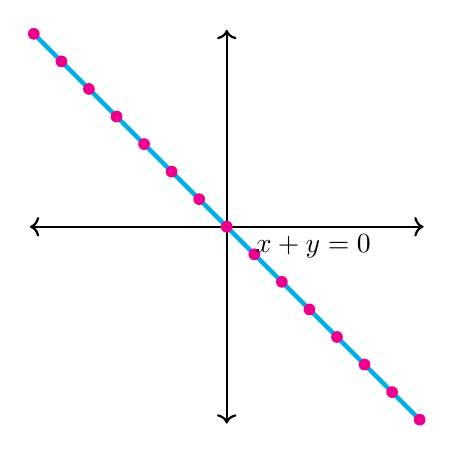
\begin{tikzpicture}[scale=0.5]
\draw[color=cyan, ultra thick] (-5,5) -- (5,-5);
\draw[color=black, thick,->] (0,0) -- (5,0);
\draw[color=black, thick,->] (0,0) -- (-5,0);
\draw[color=black, thick,->] (0,0) -- (0,5);
\draw[color=black, thick,->] (0,0) -- (0,-5);
\node at (0,0) [color=magenta,circle,fill,inner sep=1.5pt]{};
\node at (-0.7,0.7) [color=magenta,circle,fill,inner sep=1.5pt]{};
\node at (-1.4,1.4) [color=magenta,circle,fill,inner sep=1.5pt]{};
\node at (-2.1,2.1) [color=magenta,circle,fill,inner sep=1.5pt]{};
\node at (-2.8,2.8) [color=magenta,circle,fill,inner sep=1.5pt]{};
\node at (-3.5,3.5) [color=magenta,circle,fill,inner sep=1.5pt]{};
\node at (-4.2,4.2) [color=magenta,circle,fill,inner sep=1.5pt]{};
\node at (-4.9,4.9) [color=magenta,circle,fill,inner sep=1.5pt]{};
\node at (0.7,-0.7) [color=magenta,circle,fill,inner sep=1.5pt]{};
\node at (1.4,-1.4) [color=magenta,circle,fill,inner sep=1.5pt]{};
\node at (2.1,-2.1) [color=magenta,circle,fill,inner sep=1.5pt]{};
\node at (2.8,-2.8) [color=magenta,circle,fill,inner sep=1.5pt]{};
\node at (3.5,-3.5) [color=magenta,circle,fill,inner sep=1.5pt]{};
\node at (4.2,-4.2) [color=magenta,circle,fill,inner sep=1.5pt]{};
\node at (4.9,-4.9) [color=magenta,circle,fill,inner sep=1.5pt]{};
\node at (2.2,-0.5) {$x+y=0$};
\end{tikzpicture}
\caption*{Subgroup, shown in pink, of $\{(x,y) \in \R^2: x+y=0\}$}
\end{figure}}
\begin{prob}\label{prob:almostunittheorem} $\Ll(\Uu)= \{\mathbf{0}\}$ or $\Ll(\Uu)$ is infinite cyclic. 
\end{prob}


\setlength{\tabcolsep}{12pt}
\begin{table}[b]
    \begin{minipage}{.5\linewidth}
      \centering
        \begin{tabular}{rr}\toprule
        \multicolumn{1}{r}{$D$} & \multicolumn{1}{r}{$\mu$}\\ \cmidrule(lr){1-1}\cmidrule(lr){2-2} %\morecmidrules \cmidrule(lr){1-1}\cmidrule(lr){2-2}
            2 & $1+\theta+\theta^2$ \\
            3 & $4+3\theta+2\theta^2$ \\
            4 & $5 + 3\theta + 2\theta^2$ \\
            5 & $41 + 24\theta + 14\theta^2$ \\
            6 & $109 + 60\theta + 33 \theta^2$ \\\bottomrule
        \end{tabular}
    \end{minipage}%
    \begin{minipage}{.5\linewidth}
      \centering
        \begin{tabular}{rr}\toprule
            \multicolumn{1}{r}{$D$} & \multicolumn{1}{r}{$\mu$}\\ \cmidrule(lr){1-1}\cmidrule(lr){2-2} %\morecmidrules \cmidrule(lr){1-1}\cmidrule(lr){2-2}
            7 & $4 + 2\theta + \theta^2$ \\
            9 & $4 + 2 \theta + \theta^2$ \\
            10 & $181 + 84 \theta + 39\theta^2$\\
            11 & $89 + 40 \theta + 18\theta^2$ \\
            12 & $9073 + 3963\theta + 1731\theta^2$\\\bottomrule       \end{tabular}
    \end{minipage} 
        \caption*{Generators $\mu$ of $\Uu$ for the first several cubefree $D>1$.}
\end{table}

Since $\Ll$ is an isomorphism from $\Uu$ onto $\Ll(\Uu)$, we conclude from Problem \ref{prob:almostunittheorem} that  $\Uu=\{1\}$ or $\Uu$ is infinite cyclic. With a bit more work, we could show that the second possibility always holds. (Look up the proof of \textsf{Dirichlet's unit theorem} in your favorite algebraic number theory textbook.) For our purposes, having $\Uu =\{1\}$ would only make life easier, so we do not worry about eliminating that (pseudo)possibility.

\section*{A Finiteness Theorem for a Cubic Analogue of Pell's Equation} 
The next two exercises outline a proof of the following theorem.

\begin{thm} Let $D$ be a cubefree integer with $D>1$. Then $x^3-Dy^3=1$ has finitely many integer solutions $x,y$.
\end{thm}

Restricting to cubefree $D> 1$ is not significant: Any $D \in \Z^{+}$ can be factored as $D = D_0 D_1^3$, where $D_0, D_1$ are positive integers with $D_0$ cubefree. Distinct solutions to $x^3-D y^3=1$ give rise to distinct solutions to $x'^3 - D_0 y'^3=1$ (take $x'=x$, $y'=D_1 y$). When $D_0 > 1$, the theorem applies to show that the latter equation has finitely many integer solutions; hence, so does the former. Finally, if $D_0=1$, then $D$ is a cube and each solution to $x^3-Dy^3=1$ yields a way of writing $1$ as a difference of two cubes. But there is only one of these: $1 = 1^3-0^3$. (Why?) So the conclusion of the theorem actually holds for all $D \in \Z^{+}$.

This theorem, first shown by Thue in 1909, stands in sharp contrast with the situation for the classical (quadratic) Pell equation $x^2-Dy^2=1$, which has infinitely many integer solutions for all nonsquare $D\in \Z^{+}$.

We continue with the notation of the last section.  From our work there, \begin{equation}\tag{$\dagger$} x^3-Dy^3=1  \Longleftrightarrow \Nm(x-y\theta)=1\Longleftrightarrow x-y\theta \in \Uu.\end{equation}

If $\Uu=\{1\}$, the equation $x-y\theta\in \Uu$ forces $x=1, y=0$, and we are done proving the theorem already! That was too easy, so we suppose $\Uu = \langle \mu\rangle$, where $\mu$ has infinite order. We may assume that $\mu  > 1$, by replacing $\mu$ with $1/\mu$ if necessary. 

From ($\dagger$), the solutions $x,y \in \Z$ to $x^3-Dy^3= 1$ are in one-to-one correspondence with integers $n$ for which $\mu^n$ has vanishing $\theta^2$-coefficient when written with respect to the basis $1,\theta,\theta^2$. From Problem \ref{prob:coeffsisolate}, if $\mu^n = X + Y\theta + Z\theta^2$, then 
\[ 3Z \theta^2 = \mu^n + \omega \mu'^n + \omega^2 \mu''^n. \]
So we are looking for $n\in \Z$ where $\mu^n + \omega \mu'^n + \omega^2 \mu''^n=0$. This calls to mind Exercise \ref{ex:KC}.

\begin{prob}\label{ex:cubicpell}\label{prob:all1} Let $L = \Q(\theta, \omega)$ ($= \Q(\theta, \theta', \theta'')$). Fix an odd prime $p$ for which $L$ embeds into $\Q_p$. Then $|\theta|_p = |\omega|_p= |\mu|_p = |\mu'|_p =|\mu''|_p = 1$. That is, all of $\theta,\omega, \mu, \mu', \mu''$ belong to $\Z_p^{\times}$.

{\scriptsize Here we abuse notation slightly, using the same symbols for elements of $L$ and corresponding elements of $\Q_p$ under our embedding.}
\end{prob}

\begin{prob}\label{ex:cubicpell2}\label{prob:notconstantzero} Let $L$ and $p$ be as in Exercise \ref{ex:cubicpell}. We would like to apply Exercise \ref{ex:KC} to detect the vanishing of $\mu^n + \omega \mu'^n + \omega^2 \mu''^n$ but there is no reason to expect that $\mu, \mu', \mu'' \in 1 + p\Z_p$. 

To deal with this, set $\nu:= \mu^{p-1}, \nu':= \mu'^{p-1}, \nu'':= \mu''^{p-1}$. These belong to $1+p\Z_p$ by Fermat's little theorem. Writing $n=(p-1)m+r$, 
\[ \mu^n + \omega \mu'^n + \omega^2 \mu''^n= \mu^{r} \nu^m+ \omega \mu'^{r} \nu'^{m} + \omega^2 \mu''^{r} \nu''^{m}. \]
For each fixed $r$, there is some $m \in \Z$ where the right-hand side is nonzero (check this!). Hence, the RHS vanishes for only finitely many $m \in \Z$ (Exercise \ref{ex:KC}). The Theorem follows.\index{cubic Pellian equation}\index{$x^3-Dy^3=1$, finiteness of solutions}\

{\scriptsize Much more is known. For instance, Delaunay and Nagell showed (independently) that $x^3-Dy^3=1$ has at most one integer solution $\ne (1,0)$.}
\end{prob}

\begin{prob}[a striking corollary]\label{prob:strikingcor} Let $\mathcal{P}$ be a finite set of primes and let $\mathcal{D}=\{\prod_{p \in \mathcal{P}} p^{e_p}: \text{each $e_p =0,1,\text{ or }2$}\}$. If $n \in \Z^{+}$ and $n^3+1$ has all prime factors from $\mathcal{P}$, then $(-n)^3-Dy^3=1$ for some integer $y$ and some $D\in \mathcal{D}\setminus\{1\}$.

Deduce: The largest prime factor of $n^3+1$ tends to infinity with $n$.

{\scriptsize By more elaborate methods, Siegel showed that the largest prime factor of $f(n)$ tends to infinity whenever $f(T)\in \Z[T]$ is nonconstant with at least two distinct complex roots.}
\end{prob}



\setcounter{chapter}{13}
\setcounter{chapter}{13}
\chapter*{$p$-Set \#13}\label{chap:chap13}
\addcontentsline{toc}{chapter}{Set \#13}
\markboth{Set \#13}{Set \#13}

\epigraph{\textsc{Narrator}: And so we come to the last chapter in which Christopher Robin and Pooh come to the enchanted place and we say goodbye.

\textsc{Winnie the Pooh}: Goodbye? Oh no please can't we go back to page one and do it all over again?

\textsc{Narrator}: Sorry Pooh. But all stories have an ending you know.

\textsc{Winnie the Pooh}: Oh bother.}
{{The Many Adventures of Winnie the Pooh}}


\section*{Bern, Baby, Bern!}

For each integer $u$ not divisible by $p$, let $\omega(u)$ denote the $(p-1)$th root of unity in $\Q_p$ congruent to $u$ modulo $p\Z_p$ (see Problem \ref{prob:teichmuller}).\index{Teichm\"{u}ller representatives} Define $\vartheta(u)\in \Z_p$ by the equation $\omega(u) = u + p \vartheta(u)$.

\begin{prob}\label{prob:fundamentalidentity} For each $k\in \Z^{+}$:~  $\sum_{u=1}^{p-1} \omega(u)^{k} = \one_{p-1\mid k} (p-1)$.
\end{prob}

\begin{prob}\label{prob:betakintegral} Let $\beta_k = \frac{B_k}{k} - \frac{\one_{p-1\mid k}(p-1)}{pk}$. For each $k \in \Z^{+}$: \\
\[ \beta_k + \sum_{0 < j \le k} \binom{k-1}{j-1} B_{k-j}\frac{p^{j}}{j(j+1)}+\sum_{0 < j \le k}\binom{k-1}{j-1}\frac{p^{j-1}}{j}\sum_{u=1}^{p-1}u^{k-j}\theta(u)^j =0. \]
\end{prob}

\begin{prob}\label{prob:adams} Assume $p$ is odd. Then $\beta_k \in \Z_{p}$ for every $k\in \Z^{+}$. As a consequence, $\frac{B_k}{k} \in \Z_{p}$ whenever $p-1\nmid k$ \textbf{(Adams)}.\index{Bernoulli numbers!Adams' theorem}
\end{prob}


\begin{prob}\label{prob:prekummer} Assume $p\ge 5$. Then $\beta_{k}+\sum_{u=1}^{p-1} u^{k-1}\vartheta(u) \in p\Z_{p}$ for each $k \in 2\Z^{+}$.
\end{prob}

\begin{prob}[Kummer]\label{prob:kummer} If $k,k'$ are even positive integers with $k\equiv k'\pmod{p-1}$, and $p-1\nmid k$, then $\frac{B_k}{k}\equiv \frac{B_{k'}}{k'}\pmod{p\Z_{p}}$.\index{Bernoulli numbers!Kummer's congruence}
\end{prob}

{\scriptsize For example, $\frac{B_{4}}{4}= -\frac{1}{120}$ and $\frac{B_{10}}{10}= \frac{1}{132}$ are congruent mod $7\Z_{7}$. In fact, $\frac{B_{4}}{4} - \frac{B_{10}}{10} = 7 \cdot -\frac{1}{440}$.}

\begin{prob}[Glaisher]\label{prob:glaisherharmonic}\index{harmonic number}\index{Bernoulli numbers!associated congruence for $H_{p-1}$}  Let $p \ge 5$, and put $k = \varphi(p^3)-1$. Modulo $p^3 \Z_{p}$, 
\[ H_{p-1} \equiv \sum_{n=1}^{p-1} n^{k} \equiv  k\frac{p^2}{2} B_{k-1} \equiv -\frac{p^2}{3} B_{p-3}.\]
(Here, as usual, $H_{p-1} = 1 + \frac12 + \dots + \frac1{p-1}$.) Therefore: $p^3$ divides the numerator of $H_{p-1}$ $\Longleftrightarrow$ $p$ divides the numerator of $B_{p-3}$. (Compare with Problem \ref{prob:wolstenholme}.)\index{Wolstenholme prime} 

{\scriptsize Primes $p$ dividing the numerator of $B_{p-3}$ are known as \textsf{Wolstenholme primes}. The only examples not exceeding $10^{11}$ are 	$\numprint{16843}$ and $\numprint{2124679}$.}
\end{prob}


\section*{Strassmann Series}
Let $F(T) = \sum_{k\ge 0} a_k T^k \in \Q_p[[T]]$ be a Strassmann series where not all $a_k=0$. Since $a_k\to 0$ in $\Q_p$, there is a largest nonnegative integer $K$ with
\[ a_K = \max_{k\ge 0} |a_k|_{p}. \]
We refer to $K$ as the \textsf{Strassmann degree} of $F(T)$.\index{Strassmann degree}\index{Strassmann series!Strassmann degree of} For example, $p+T+\sum_{k\ge 2} p^{\lfloor \sqrt{k}\rfloor} T^k$ has Strassmann degree $1$, while $\sum_{k\ge 0} k!\cdot T^k$ has Strassmann degree $p-1$.

 \begin{prob}\label{prob:strassdivide} Let $F(T) = \sum_{k \ge 0} a_k T^k$ be a Strassmann series with a zero $r \in \Z_p$. For all $x \in \Z_p$, we have $F(x) = (x-r) G(x)$, where 
\[ G(T) = \sum_{j\ge 0} b_j T^j, \quad\text{with}\quad b_j:= \sum_{k > j}a_k r^{k-1-j}. \]
Moreover, if $F(T)$ has Strassmann degree $K\ge 1$, then $G(T)$ is Strassmann with Strassmann degree $K-1$.
\end{prob}

\begin{prob}[Strassmann's Theorem]\label{ex:strassthm}\index{Strassmann's theorem}\index{Strassmann series!number of zeros bounded by Strassmann degree} Let $F(T)$ be a Strassmann series with Strassmann degree $K$. Then $F(x)=0$ for at most $K$ distinct values of $x \in \Z_p$.
\end{prob}

\section*{Ramanujan's Conjecture Revisited}\index{Ramanujan--Nagell equation}
We finally return to the study of the equation $x^2+7= 2^m$ initiated in Exercise \ref{ex:ram1}. By that problem, to establish Ramanujan's conjecture it suffices to show that there are no $n>13$ with $\frac{\alpha^n-\beta^n}{\alpha-\beta} = \pm 1$. Here $\alpha = \frac{1+\sqrt{-7}}{2}$ and $\beta =\frac{1-\sqrt{-7}}{2}$.

The quadratic field $\Q(\sqrt{-7})$ can be viewed as a subfield of $\Q_{11}$, identifying $\sqrt{-7}$ with the square root of $-7$ in $\Z_{11}$ that is congruent to $2$ modulo $11\Z_{11}$. By hand, or with the aid of software such as PARI/GP, one computes that  \[ \sqrt{-7} = 2 + 8\cdot 11 + 8 \cdot 11^2 + 7 \cdot 11^3 + 10\cdot 11^4 + 1\cdot 11^5 + \dots,  \]
where $\dots$ suppresses a quantity with $11$-adic absolute value at most $11^{-6}$. Then
\begin{align*} \alpha &= 7 + 9\cdot 11 + 9\cdot 11^2 + 3\cdot 11^3 + 5\cdot 11^4 + 6\cdot 11^5 + \dots,\\
\beta &= 5 + 1\cdot 11 + 1\cdot 11^2 + 7\cdot 11^3 + 5\cdot 11^4 + 4\cdot 11^5 + \dots.\end{align*}

We study the equation $\frac{\alpha^n  - \beta^n}{\alpha-\beta}= \pm 1$ by the method of Exercise \ref{ex:cubicpell2}. Put $A=\alpha^{10}$ and $B = \beta^{10}$, so that $A= 1+a, B=1+b$ for 
\begin{align*}
 a&= 7\cdot 11 + 1\cdot 11^2 + 1\cdot 11^3 + 7\cdot 11^4 + 5\cdot 11^5 + \dots,\\
 b&= 9\cdot 11 + 9\cdot 11^2 + 9\cdot 11^3 + 3\cdot 11^4 + 5\cdot 11^5 +\dots,
\end{align*}
both of which belong to $11\Z_{11}$. Write $n = 10m+r$, where $r \in \{0,1,\dots,9\}$. Then 
\begin{align*} \frac{\alpha^n - \beta^n}{\alpha-\beta} = \pm 1 &\Longleftrightarrow \alpha^n-\beta^n = \pm (\alpha-\beta) \\
&\Longleftrightarrow \alpha^{r} (1+a)^m - \beta^{r} (1+b)^m \mp (\alpha-\beta) = 0.
\end{align*}

For each $r\in \{0,1,\dots,9\}$ and each choice of $\pm$ sign, define $$F_{r,\pm}(T) = \alpha^{r}\,\Binom(1+a;T) - \beta^{r}\,\Binom(1+b;T) \mp (\alpha-\beta),$$ so that $F_{r,\pm}(m) = \alpha^{r} (1+a)^m - \beta^{r} (1+b)^m \mp (\alpha-\beta)$ for all $m \in \Z$. %(Look back at Exercises \ref{ex:binomialseries} and \ref{ex:binom2} for the definition of $\Binom$.) 

Each of our 20 power series $F_{r,\pm}(T)$ is a Strassmann series. For every one of these, we will apply Strassmann's Theorem (Exercise \ref{ex:strassthm}) to bound the number of zeros in $\Z_p$.

\begin{prob}\label{prob:constantcheck} The constant term of $F_{r,\pm}(T)$ is $\alpha^r-\beta^r \mp (\alpha-\beta)$, which vanishes when \[ (r,\pm) \in \{(1,+), (2,+), (3,-), (5,-)\} \] and is an $11$-adic unit in the other sixteen cases. Every nonconstant coefficient of every $F_{r,\pm}(T)$ is a multiple of $11$. Hence, $F_{r,\pm}(T)$ has no zero in $\Z_{11}$ except possibly for the four displayed values of $(r,\pm)$.
\end{prob}

\begin{prob}\label{prob:easycases} All of $F_{1,+}(T)$, $F_{2,+}(T)$, $F_{5,-}(T)$ have their $T$-coefficients multiples of $11$ but not $11^2$. Their Strassmann degrees are all $1$.
\end{prob}           

\begin{prob}\label{prob:annoyingcase} $F_{3,-}(T)$ has a $T$-coefficient that vanishes mod $11^2$. Its $T^2$-coefficient is a multiple of $11^2$ but not $11^3$. Its Strassmann degree is $2$.
\end{prob}

\begin{prob}\label{ex:finalram} There are at most $3\cdot 1 + 2=5$ integers $n$ with $\frac{\alpha^n-\beta^n}{\alpha-\beta}=\pm 1$. We know five such integers --- $n=1, 2, 3, 5$, and $13$ --- so those must be all of them.
\end{prob}

\begin{rmk} The choice to work in $\Q_p$ for $p=11$ was fortuitous. The next prime after $11$ for which $-7$ is a quadratic residue is $p=23$. If we had elected to embed $\Q(\sqrt{-7})$ into $\Q_{23}$, we would have to bound the number of zeros of $2\cdot 22 = 44$ Strassmann series. One of those would correspond to the equation $\frac{\alpha^{22m+12}-\beta^{22m+12}}{\alpha-\beta}=- 1$. If you approximate the coefficients sufficiently to apply Strassmann's theorem, you'll find that this series has \underline{at most one} zero $m \in \Z_p$; hence, $\frac{\alpha^{22m+12}-\beta^{22m+12}}{\alpha-\beta}=- 1$ has at most one integer solution $m$. But in fact (as we know after Exercise \ref{ex:finalram}), there are \underline{zero} integers $m$ satisfying the equation. So working in $\Q_{23}$, we fail to rule out an extraneous zero. What's going on in this instance is that there really \emph{is} an $m \in \Z_{23}$ where the associated power series vanishes --- but this $m$ does not belong to $\Z$! \end{rmk}
 
\setcounter{part}{1}
%%%%%%%%%%%%%%%%%%%%%%%% part.tex %%%%%%%%%%%%%%%%%%%%%%%%%%%%%%%%%%
%
% sample part title
%
% Use this file as a template for your own input.
%
%%%%%%%%%%%%%%%%%%%%%%%% Springer-Verlag %%%%%%%%%%%%%%%%%%%%%%%%%%


\part{Solutions, Discussion, and \pp s}


\chapter*{Solutions to Set \#1}
\addcontentsline{toc}{chapter}{Solutions to Set \#1}
\markboth{Solutions to Set \#1}{Solutions to Set \#1}
\label{set0sols}

\begin{sol}{prob:01} 
    \begin{enumerate}
        \item[(a)] First off, $|1|^2 = |1\cdot 1|=|1|$ and $|1| > 0$ (from (i)). Thus, $|1| = 1$. Next, $|-1|^2 = |(-1) (-1)| = |1| = 1$. As $|-1| > 0$, we conclude that $|-1|=1$.
\item[(b)] The proof is the same for the ``standard'' absolute value: By the triangle inequality, $|x| = |(x-y)+y| \le |x-y| + |y|$. Now rearrange.
\item[(c)] Since $|y^{-1}|\cdot |y|= |y^{-1}\cdot y| = |1| = 1$, we have $|y^{-1}| = |y|^{-1}$. So $|xy^{-1}| = |x||y^{-1}| = |x||y|^{-1}$, as claimed.
    \end{enumerate}
\end{sol}

\begin{sol}{prob:02}  Property (i) in the absolute value definition is clear. Property (ii) is also easy: When $x+y=0$, the inequality is obvious. Otherwise, either $x$ or $y$ is nonzero, so that $|x|$ or $|y|$ is $1$. Hence, $1= |x+y| \le |x| + |y|$. To prove (iii), take cases: If $x$ and $y$ are nonzero, both sides are $1$, otherwise both sides are $0$. In this last step we use that fields are integral domains.
\end{sol}

\begin{sol}{prob:03} Property (i) is again clear. Of the remaining two properties, (iii) is quicker to dispense with: If $x$ or $y$ is zero, both sides of (iii) vanish. Otherwise, write $x= p^{v_p(x)} \frac{a}{b}$ and $y=p^{v_p(y)} \frac{c}{d}$, where $p$ does not divide any of $a,b,c,d$. Then $xy = p^{v_p(x)+v_p(y)} \frac{ac}{bd}$, and $p$ does not divide either of $ac$ or $bd$. Hence, $v_p(xy) = v_p(x) + v_p(y)$ and $|xy|_p = p^{-v_p(x)} p^{-v_p(y)} = |x|_p |y|_p$.

To prove (ii) we have to work a bit harder. If $x$, $y$, or $x+y$ is zero, (ii) is trivial. Otherwise, write $x= p^{v_p(x)} \frac{a}{b}$ and $y=p^{v_p(y)} \frac{c}{d}$ as above. The symmetry of (ii) in $x$ and $y$ allows us to assume $v_p(x) \le v_p(y)$. Then $x+y= p^{v_p(x)} \left(\frac{a}{b} + p^{v_p(y)-v_p(x)} \frac{c}{d}\right)$. Since $p^{v_p(y)-v_p(x)}\in \Z$, we can express $p^{v_p(y)-v_p(x)}\frac{c}{d}$ as a fraction with denominator $d$. Hence, $\frac{a}{b} + p^{v_p(y)-v_p(x)} \frac{c}{d} = \frac{N}{bd}$ for some nonzero $N\in \Z$. Write $N = p^{w} N'$, where $w$ is a nonnegative integer and $N'\in \Z$ is not divisible by $p$. Then $x+y = p^{v_p(x)+w} \frac{N'}{bd}$, where neither $N'$ nor $bd$ is divisible by $p$. Hence, $v_p(x+y) = v_p(x) + w \ge v_p(x)$, and $|x+y|_{p} = p^{-v_p(x)} p^{-w} = |x|_p p^{-w} \le |x|_p \le |x|_p + |y|_p$.
\end{sol}


\begin{sol}{prob:05} This is implicit in our solution to Problem \ref{prob:03}.
\end{sol}

\begin{sol}{prob:04} We may assume without loss of generality that $|x| > |y|$. A direct application of the strong triangle inequality gives $|x+y| \le \max\{|x|,|y|\} = |x|$. The strong triangle inequality also implies that $|x| = |(x+y) + (-y)| \le \max\{|x+y|,|-y|\} = \max\{|x+y|,|y|\}$. (We use in this last step that $|-y| = |y|$, which follows from $|-1|=1$.) Since $|x| > |y|$, the maximum here cannot be $|y|$. So it must be $|x+y|$, yielding $|x| \le |x+y|$. Hence, $|x+y| = |x|$.  
\end{sol}


\begin{sol}{prob:06} Since $|2| \le 1$, we see that $|2^{e_1} + \dots + 2^{e_n}| \le  |2|^{e_1} + \dots + |2|^{e_n} \le 1  +\dots + 1 = n$.
To conclude, notice that (a) every positive integer less than $2^n$ is a sum of at most $n$ powers of $2$ (e.g., use the binary representation), while (b) $\sum_{0 \le k \le n} \binom{n}{k}=2^n$, so that $\binom{n}{k} < 2^n$ for every $k$.
\end{sol}

\begin{sol}{prob:07}\index{absolute value!product formula on $\Q$}\index{product formula for absolute values on $\Q$} Write $x = \pm \frac{a}{b}$ where $a$ and $b$ are relatively prime positive integers. Since $a$ and $b$ share no prime factors,
\[ \prod_{p\text{ prime}} |x|_p = \prod_{p \text{ prime}} \left(|a|_p |b|_p^{-1}\right) = \prod_{p\mid a} p^{-v_p(a)} \prod_{p \mid b} p^{v_p(b)} = |a|_{\infty}^{-1} |b|_{\infty},\]
which is the multiplicative inverse of $|a|_{\infty} |b|_{\infty}^{-1} = |x|_{\infty}$.
\end{sol}

\begin{challenge}[simultaneous approximation]\index{simultaneous approximation} The product formula suggests that $|\cdot|_{\infty}$, $|\cdot|_2$, $|\cdot|_3$, $|\cdot|_5, \dots$ ``know about each other.'' The situation is very different if one considers only a finite subset of these absolute values. Make this precise by proving the following independence statement.

Let $\Pp$ be a finite set of primes. Choose rational numbers $x_p$ for each prime $p\in \Pp$, alongside a rational number $x_{\infty}$. For each $\epsilon > 0$, there is a rational number $x$ satisfying 
\[ |x - x_p|_p < \epsilon\quad\text{for all $p \in \mathcal{P}$}, \quad\text{as well as}\quad |x-x_{\infty}|_{\infty} <\epsilon. \]
\end{challenge}

\begin{sol}{prob:08} We begin by demonstrating a fabulously useful formula of Legendre\index{Legendre's formula for $v_p(n"!)$}: For each prime $p$ and nonnegative integer $n$,
\[ v_p(n!) = \sum_{1 \le m \le n} v_p(m) = \sum_{1 \le m \le n} \sum_{\substack{p^k \mid m \\ k \ge 1}} 1 = \sum_{k \ge 1} \sum_{\substack{1 \le m \le n \\ p^k \mid m}} 1 = \sum_{k \ge 1} \left\lfloor \frac{n}{p^k}\right\rfloor. \]

When $n>0$, it follows that $v_p(n!) < \sum_{k \ge 1} \frac{n}{p^k} = \frac{n}{p-1}$. (The inequality is surely strict, as $\lfloor n/p^k\rfloor < n/p^k$ whenever $p^k > n$.) Therefore, $|n!|_{p} = p^{-v_p(n!)} > p^{-n/(p-1)}$.\index{absolute value!of factorials}
\end{sol}

\begin{challenge}[following up on Legendre's formula] Let $p$ be a prime. For each nonnegative integer $n$, expand $n$ in base $p$: write $n = n_0 + n_1 p + n_2 p^2 + \dots$, where each $n_i \in \{0,1,2,\dots,p-1\}$ and all but finitely many $n_i=0$. Set $s_p(n) = n_0 + n_1 + n_2 + \dots$.
\begin{enumerate} 
\item[(a)] Show that $v_p(m) = \frac{1}{p-1}(s_p(m-1)-s_p(m)+1)$ for every positive integer $m$. Deduce that $v_p(n!) = \frac{1}{p-1}(n - s_p(n))$ for all nonnegative integers $n$ (an alternative form of Legendre's formula).
\item[(b)] Prove that $n!/(-p)^{v_p(n!)} \equiv n_0! n_1! n_2! n_3! \cdots\pmod{p}$ for all nonnegative $n\in\Z$. (Anton \cite{anton}, Stickelberger \cite[pp.~342--343]{stickelberger}, Hensel \cite{hensel})
\end{enumerate}
\end{challenge}


\begin{sol}{prob:09} We interpret ``grows faster'' to mean that $n!/C^{n}$ tends to infinity. To prove that, we may (in fact, should!) assume that $C>0$. A (canonical) application of the ratio test shows that $\sum_{n\ge 0} C^n/n!$ converges. (It converges to $\e^C$ but we do not need that here.) So its terms must tend to $0$. Since $C^n/n!$ is positive for each $n$, we deduce that $n!/C^n\to\infty$.

On the other hand, if there are only finitely many primes, then $n! = |n!|_{\infty} = \prod_{p} |n!|_{p}^{-1} \le \prod_{p} p^{n/(p-1)} = (\prod_{p} p^{1/(p-1)})^{n}$. That is, $n! \le C^n$ with $C := \prod_{p} p^{1/(p-1)}$. Contradiction!
\end{sol}

\begin{challenge}[Skolem \cite{skolem}] Show that if $p$ is prime and $n\in \Z^{+}$, either $|2^n-1|_p=1$ or $|2^n-1|_p = |2^{p-1}-1|_p |n|_p$. Deduce that if $\Pp$ is any fixed finite set of primes, then $2^n-1$ has a prime factor outside of $\Pp$ for all sufficiently large $n$. 
\end{challenge}

\begin{sol}{prob:10} Given $n \in \Z^{+}$, let $e$ be the largest nonnegative integer such that $2^{e}\le n$. Then $2^e$ is the unique integer in $[1,n]$ divisible by $2^e$. (The next smallest multiple of $2^e$ is $2^{e+1}$, but this exceeds $n$.) It follows that $|1/m|_{2} = 2^{v_2(m)}$ has a unique maximum, among $m \in [1,n]$, at $m=2^e$. By ``survival of the greatest'' (Exercise \ref{prob:05}), $|H_n|_2 = |\sum_{m \le n} 1/m|_{2} = |1/2^e|_{2}= 2^{e} > \frac{1}{2}n$. So $|H_n|_2\to\infty$.

\begin{challenge} Prove that in any nonempty set $S$ of consecutive positive integers, one element of $S$ has strictly smaller $2$-adic absolute value than all the     others. Conclude that if $S\ne\{1\}$, then $\sum_{n \in S} 1/n \notin \Z$ \textbf{(Kürschák \cite{kurschak})}.
\end{challenge} 
\end{sol}


\begin{sol}{prob:11}\index{harmonic number}\index{Wolstenholme's theorem} The stated expression for $H_{p-1}$ is immediate upon pairing the terms $\frac{1}{i}$ and $\frac{1}{p-i}$. To show $|H_{p-1}|_{p} \le p^{-2}$, we must prove that $|S|_{p} \le p^{-1}$, where $S: = \sum_{0 < i < p/2} \frac{1}{i(p-i)}$. 

We would like to evaluate $S$ modulo $p$ by reducing term-by-term. This is essentially what we will do, but since it is not immediately clear what it means to reduce a rational number mod $p$, we premultiply by $(p-1)!$. In the field $\F_p=\Z/p$, we have $\frac{(p-1)!}{i(p-i)} = (p-1)!i^{-1} (p-i)^{-1} = -(p-1)! i^{-2}$\footnote{The first equality is not  a tautology! What is being claimed is that the integer on the left has its mod $p$ reduction equal to the element of $\F_p$ on the right. The $-1$st powers indicate inverses in the field $\F_p$.} whenever $0 < i < p/2$.  Therefore (still working in $\F_p$),
\[ (p-1)!S = -(p-1)! \sum_{0 < i < p/2} i^{-2} = -\frac{1}{2}(p-1)! \sum_{i \in \F_p^{\times}} i^{-2} = -\frac{1}{2}(p-1)! \sum_{j \in \F_p^{\times}} j^{2}. \]
Here we use that $i^{-2} = (p-i)^{-2}$ and that as $i$ runs over all the nonzero elements of $\F_p$, so does $j = i^{-1}$. To finish, observe that since $p > 3$, the group $\F_p^{\times}$ has an element other than $\pm 1$. So there is an $r \in \F_p^{\times}$ with $r^2\ne 1$. Since multiplication by $r$ permutes $\F_p^{\times}$,
\[ r^2 \sum_{j \in \F_p^{\times}} j^{2} = \sum_{j \in \F_p^{\times}} (rj)^{2} = \sum_{j \in \F_p^{\times}} j^{2}, \]
forcing $\sum_{j \in \F_p^{\times}} j^2=0$ (since $r^2\ne 1$). It follows that $(p-1)!S=0$ in $\Z/p$, and so $(p-1)!S$ is a multiple of $p$. Since $p\nmid (p-1)!$, we conclude that $|S|_p = |(p-1)!|_p |S|_p = |(p-1)! S|_p \le p^{-1}$, as desired.

\begin{rmk} It is not really necessary to premultiply by $(p-1)!$. On the next problem set, we will introduce the ring $\Z_{(p)}$, whose elements are the rational numbers with denominators prime to $p$. $\Z_{(p)}$ is a local ring (in fact, domain) with unique maximal ideal $p\Z_{(p)}$, and $\Z_{(p)}/p\Z_{(p)} \cong \Z/p = \F_p$. The same argument we used to show $(p-1)!S=0$ in $\Z/p$ will show directly that $S = 0$ in $\Z_{(p)}/p\Z_{(p)}$, and this is sufficient to conclude that $|S|_p \le p^{-1}$.  
\end{rmk}
\end{sol}




\renewcommand\refname{\normalsize References}
\let\oldaddcontentsline\addcontentsline
\renewcommand{\addcontentsline}[3]{}
\begin{thebibliography}{11}
\bibitem{anton} H.~Anton, \emph{Die Elferprobe und die Proben für die Modul Neun, Dreizehn und Hunderteins.  Für Volks- und Mittelschulen}. Archiv Math. Physik \textbf{49} (1869), 241--308.

\bibitem{hensel} K.~Hensel, \emph{Über die arithmetischen Eigenschaften der Faktoriellen}. Archiv Math. Physik (third series) \textbf{2} (1902), 293--294.

\bibitem{kurschak}
J. Kürschák, \emph{A harmonikus sorról}. Mat. Fiz. Lapok \textbf{27} (1918), 299--300. 

\bibitem{skolem}
T. Skolem, \emph{On certain exponential equations}.
Norske Vid. Selsk. Forh. \textbf{18} (1945), 71--74.

\bibitem{stickelberger}
L. Stickelberger, \emph{Ueber eine Verallgemeinerung der Kreistheilung}. Math. Ann. \textbf{37} (1890), 321--367.



\end{thebibliography}
\let\addcontentsline\oldaddcontentsline


% \let\oldaddcontentsline\addcontentsline
% \renewcommand{\addcontentsline}[3]{}
% \begin{thebibliography}{11}
%         \bibitem{newman}  Donald J. Newman,
% \emph{A problem seminar}. Problem Books in Mathematics. Springer-Verlag, New York-Berlin, 1982.
%     \end{thebibliography}
% \let\addcontentsline\oldaddcontentsline



\chapter*{Solutions to Set \#2}
\addcontentsline{toc}{chapter}{Solutions to Set \#2}
\markboth{Solutions to Set \#2}{Solutions to Set \#2}
\label{set1sols}

\begin{sol}{prob:12} We have to show that for any $x,y,z\in K$, at least two of $|x-y|, |y-z|$, and $|z-x|$ coincide. This is a simple consequence of ``survival of the greatest'': If $|x-y| \ne |y-z|$, then $|z-x| = |x-z| = |(x-y) + (y-z)|= \max\{|x-y|,|y-z|\}$. This argument shows that the largest side length always appears at least twice.
\end{sol}


\begin{sol}{prob:13}\index{discs, open and closed} Suppose to start with that $z \in \Dd_{<r}(x)$. Then $|z-x_0| = |(z-x)+(x-x_0)| \le \max\{|z-x|,|x-x_0|\} < r$. Thus, $\Dd_{<r}(x) \subset \Dd_{<r}(x_0) = D$. Similarly, if $z \in D$, then $|z-x| = |(z-x_0) + (x_0-x)|\le \max\{|z-x_0|,|x_0-x|\} <r$, proving that $D \subset \Dd_{<r}(x)$. So $D = \Dd_{<r}(x)$.
\end{sol}


\begin{sol}{prob:14} Suppose that $x\in K$ belongs to the intersection of the open discs $D_0 = \Dd_{<r_0}(x_0)$ and $D_1=\Dd_{<r_1}(x_1)$. By Problem \ref{prob:13}, $D_0 = \Dd_{<r_0}(x)$ and $D_1 = \Dd_{<r_1}(x)$. Then $D_0\subset D_1$ or $D_1 \subset D_0$ according to whether $r_0 \le r_1$ or vice versa.
\end{sol}

\begin{sol}{prob:15} Let $\mathcal{R} = \{p^v: v \in \Z\}$. If $r \notin \mathcal{R}$, then $\Dd_{<r}(x_0) = \Dd_{\le r}(x_0)$, for any center $x_0$. If $r \in \mathcal{R}$, then $\Dd_{<r}(x_0) = \Dd_{\le r/p}(x_0)$ while $\Dd_{\le r}(x_0) = \Dd_{<pr}(x_0)$. 
\end{sol}

\begin{sol}{prob:16} Suppose $|\cdot|$ is an absolute value on $F= \F_{2027}$. Let $g$ be a generator of $F^{\times}$. Then $|g|^{2026} = |g^{2026}| = |1| = 1$, and so $|g|=1$. Since $g$ generates $F^{\times}$, it follows that $|x|=1$ for all nonzero $x$ in $F$. Therefore, the only absolute value on $F$ is the trivial absolute value.

This argument works for any $\F_p$, or any finite field for that matter.
\end{sol}

\begin{sol}{prob:17} Applying the binomial theorem and the triangle inequality,
\begin{multline*} |x+y|^n = \left|\sum_{k=0}^{n} \binom{n}{k} x^{k} y^{n-k}\right| \le  \sum_{k=0}^{n} \left|\binom{n}{k}\right| |x|^k |y|^{n-k} \\
\le \max\{|x|,|y|\}^{n} \sum_{k=0}^{n} \left|\binom{n}{k}\right| \le \max\{|x|,|y|\}^{n} \cdot (n+1) \max_{0\le k \le n}\left|\binom{n}{k}\right|. \end{multline*}
(Moving from the first to the second line, we used that $|x|^k |y|^{n-k} \le \max\{|x|,|y|\}^k \cdot \max\{|x|,|y|\}^{n-k} = \max\{|x|,|y|\}^n$.) 
Take $n$th roots.
\end{sol}


\begin{sol}{prob:18} Every absolute value on $\F_p(T)$ restricts to an absolute value on $\F_p$, hence is trivial on $\F_p$ (Exercise \ref{prob:16}). It follows that every binomial coefficient has absolute value at most $1$. So by Exercise \ref{prob:17}, for all $x, y \in \F_p(T)$, 
\[ |x+y| \le (n+1)^{1/n} \max\{|x|,|y|\}. \] Sending $n$ to infinity, $|x+y|\le \max\{|x|,|y|\}$. In other words, $|\cdot|$ is non-Archimedean.
\end{sol}

\begin{sol}{prob:19} We start by constructing a family of absolute values on $\F_p(T)$ parametrized by the monic irreducibles in $\F_p[T]$. 

Fix a monic irreducible $\pi \in \F_p[T]$. Every $x \in \F_p(T)^{\times}$ can be written in the form $\pi^{v} \frac{a}{b}$ where $a$ and $b$ are elements of $\F_p[T]$ not divisible by $\pi$. Here the integer $v_\pi(x):=v$ is uniquely determined by $x$ (a consequence of the unique factorization theorem for $\F_p[T]$). Fix your favorite constant $C_{\pi} > 1$. If we set $|x|_{\pi} = C_\pi^{-v_\pi(x)}$ for nonzero $x \in \F_p(T)$, and set $|0|_{\pi}=0$, then $|\cdot|_{\pi}$ is a non-Archimedean absolute value on $\F_p(T)$. The proof is more or less identical to that for $|\cdot|_p$ (see Exercise \ref{prob:03}). 

If $\pi$ and $\tilde{\pi}$ are distinct monic irreducibles in $\F_p[T]$, then $|\pi|_{\pi} = C_{\pi}^{-1} < 1$ while $|\tilde{\pi}|_{\pi} = C_{\pi}^{0} = 1$. This settles the first half of the problem.

As for the concluding question: Yes, there is such an absolute value. Fix $C_{\infty} > 1$. For $x \in \F_p(T)^{\times}$, write $x = \frac{a}{b}$ with $a, b \in \F_p[T]$. While $a$ and $b$ are not uniquely determined by this representation, the difference $\deg{a} - \deg{b}$ is independent of the choice of $a$ and $b$. We put $|x|_{\infty} = C_{\infty}^{\deg{a}-\deg{b}}$ for nonzero $x \in \F_p(T)$, taking $|0|_{\infty} = 0$. Since $|T|_{\infty} = C_{\infty} > 1$, we will be done if we show $|\cdot|_{\infty}$ is an absolute value on $\F_p(T)$.

Condition (i) in the absolute value definition (see Set \#1) is obvious. Condition (iii) follows from $\deg{uv} = \deg{u} + \deg{v}$. To prove (ii), we may assume $x,y$, and $x+y$ are nonzero. Write $x = \frac{a}{b}$ and $y= \frac{c}{d}$. Then $x+y = \frac{ad+bc}{bd}$, and
\begin{align*} \deg(ad+bc) - \deg(bd) &\le \max\{\deg(ad),\deg(bc)\} - \deg(bd) \\
&= \max\{\deg(ad) - \deg(bd),\deg(bc) -\deg(bd)\}\\
&= \max\{\deg(a)-\deg(b),\deg(c)-\deg(d)\}.
\end{align*}
Since $C_{\infty} > 1$, the inequality is preserved upon raising $C_{\infty}$ to both sides. This gives $|x+y|_{\infty} \le \max\{|x|_{\infty},|y|_{\infty}\}$, proving the strong triangle inequality.
\end{sol}

\begin{sol}{prob:20}\index{$\Z_{(p)}$, ring of $p$-integral rationals} To prove that $\Dd_{\le 1}(0)$ is a subring it is enough to argue that $1 \in \Dd_{\le 1}(0)$ and that $\Dd_{\le 1}(0)$ is closed under multiplication and subtraction. The first requirement is clear, since $|1|=1$. Closure under multiplication follows from the multiplicative property of $|\cdot|$, as the interval $[0,1]$ is closed under multiplication. Closure under subtraction is a consequence of the strong triangle inequality: If $|x|, |y| \le 1$, then $|x-y| \le \max\{|x|,|-y|\} = \max\{|x|,|y|\} \le 1$. 

By definition of the $p$-adic absolute value, $x \in \Z_{(p)}$ if and only if $x = p^{v} a/b$ for some nonnegative integer $v$ and some $a,b\in \Z$ not divisible by $p$. This happens precisely when the denominator of $x$ in lowest terms is not a multiple of $p$.
\end{sol}

\begin{sol}{prob:21} Write $x=a/b$ in lowest terms, with $b>0$. By Problem \ref{prob:20}, $x \in \bigcap_{p\text{ prime}} \Z_{(p)}$ $\Longleftrightarrow$ $b$ has no prime factors $\Longleftrightarrow b= 1 \Longleftrightarrow x \in \Z$. So $\bigcap_{p\text{ prime}} \Z_{(p)}=\Z$.
\end{sol}

\begin{sol}{prob:22} Let $0 < k < p$. Working modulo $p$,
\begin{align*} (k-1)! \binom{p-1}{k-1} &= (p-1)(p-2)\cdots(p-(k-1)) \\ &\equiv (-1)(-2)\cdots(-(k-1)) \\
&\equiv (-1)^{k-1} (k-1)!.
\end{align*}
Since $p \nmid (k-1)!$, we conclude that $\binom{p-1}{k-1} \equiv (-1)^{k-1}\pmod{p}$. Write $\binom{p-1}{k-1} = (-1)^{k-1} + pr$, where $r \in \Z$. Then $\binom{p}{k}=\frac{p}{k}\binom{p-1}{k-1}  = p\frac{(-1)^{k-1}}{k} + p^2\frac{r}{k}$. Hence, working in the ring $\Z_{(p)}$, 
\[ \binom{p}{k} \equiv p \frac{(-1)^{k-1}}{k} \pmod{p^2 \Z_{(p)}}. \]
We have made sense of the claimed congruence mod $p^2$ by interpreting it --- nay, proving it --- as a congruence modulo the ideal $p^2 \Z_{(p)}$ of the ring $\Z_{(p)}$.
% Let $\phi$ be homomorphism from $\Z \to \Z_{(p)}/p^2\Z_{(p)}$ mapping $a$ to $a\bmod{p^2\Z_{(p)}}$. The map $\phi$ is onto: If $a, b \in \Z$ with $b$ not divisible by $p$, let $B \in \Z$ be an inverse of $b$ modulo $p^2$. Then $aB-\frac{a}{b}= \frac{aBb-a}{b} = p^2\frac{(aBb-a)/p^2}{b} \in p^2 \Z_{(p)}$, so that $\phi(aB) = \frac{a}{B}\bmod{p^2 \Z_{(p)}}$. Furthermore, for $a\in \Z$,
% \[ a \in \mathrm{ker}(\phi) \Longleftrightarrow a/p^2 \in \Z_{(p)} \Longleftrightarrow |a/p^2|_{p} < 1 \Longleftrightarrow |a|_p < p^{-2}  
% \Longleftrightarrow p^2 \mid a. \]
% Thus, $\ker(\phi) = p^2\Z$. We conclude that $\phi$ induces an isomorphism $\Z/p^2 \cong \Z_{(p)}/p^2 \Z_{(p)}$. 
\end{sol}

\begin{sol}{prob:23} Summing the congruence $\binom{p}{k} \equiv p \frac{(-1)^{k-1}}{k}\pmod{p^2\Z_{(p)}}$ over integers $0 < k < p$ yields $2^p-2 \equiv p \sum_{0 < k < p} (-1)^{k-1}/k \pmod{p^2 \Z_{(p)}}$. Dividing by $p$,
\[ \frac{2^p-2}{p} \equiv 1-\frac{1}{2}+\frac{1}{3}-\frac{1}{4}+\dots-\frac{1}{p-1} \pmod{p\Z_{(p)}}. \]
The left and right-hand sides of the displayed congruence have difference smaller than $1$ in terms of $p$-adic absolute value. So by the strong triangle inequality, one side has absolute value $<1$ if and only if the other does. The solution is concluded by observing that $|\frac{2^p-2}{p}|_p < 1$ $\Longleftrightarrow$ $p^2 \mid 2^p-2$.
\end{sol}

\begin{sol}{prob:24} Since $F$ has finitely many complex roots, we can fix $n_0 \in \Z$ with $F(n_0) \ne 0$. Replacing $F(T)$ with $F(T+n_0)$, we may assume that $F(T)$ has nonzero constant term $a_0$ (say). Then $F(a_0 T) = a_0 G(T)$ for some nonconstant $G(T) \in \Z[T]$ with $G(0)=1$.

Let $\mathcal{P}$ be the set of primes dividing $G(n)$ for some integer $n$. Every prime dividing a value of $G$ also divides a value of $F$, so it suffices to prove $\mathcal{P}$ is infinite.

We mimic Euclid. Suppose $p_1,\dots,p_k$ is any finite list of primes in $\mathcal{P}$. We choose an integer $m$ with $|G(mp_1\cdots p_k)|>1$. (Such an $m$ surely exists, as the inequality excludes no more than $3\deg{G}$ values of $m$.) Then $G(mp_1\cdots p_k)$ is divisible by \emph{some} prime $p$, but
\[ G(m p_1\cdots p_k) \equiv G(0) \equiv 1 \pmod{p_i} \]
for each $i=1,2,\dots, k$. So there is a prime $p\in \mathcal{P}$ not on our list. As this is true no matter what finite list we start with, $\mathcal{P}$ is infinite.
\end{sol}

\begin{challenge} Let $\mathcal{P}$ be a finite set of primes, say $\#\mathcal{P}=k$. Show that there are positive constants $c$ and $x_0$ such that, for every real number $x\ge x_0$,
\[ \#\{n \in \Z: |n|\le x\text{ and } p\mid n \Rightarrow p \in \mathcal{P}\} \le c (\log x)^{k}. \]
Use this to give another solution to Problem \ref{prob:24}.
\end{challenge}


\begin{challenge}[Bauer \cite{bauer}; {see also Nagell \cite[\S49, pp.\ 168--169]{nagell}}] Let $F(T)$ be a nonconstant polynomial with integer coefficients. Suppose that $F$ has a real root of odd multiplicity. Show that for each integer $m\ge 3$, there are infinitely many primes $p\not\equiv1\pmod{m}$ for which $F$ has a root mod $p$.
\end{challenge}

\begin{sol}{prob:25} Suppose $p$ is odd. If $p\mid n^4+1$, then  $n^4\equiv -1\pmod{p}$ and $n^8 \equiv 1\pmod{p}$. Since $-1\not\equiv 1\pmod{p}$, the order of $n$ modulo $p$ divides $8$ but does not divide $4$ --- so it must be precisely $8$. As the order is always a divisor of $p-1$, we conclude that $p\equiv 1\pmod{8}$. 

To obtain infinitely many primes $p\equiv 1\pmod{8}$, apply Problem \ref{prob:24}.
\end{sol}

\begin{sol}{prob:26} If $p\mid (2n+1)^2-2$, then $p$ is odd and $2$ is a square modulo $p$. By elementary number theory, $p\equiv \pm 1\pmod{8}$. 

For each $n \in \Z^{+}$, the integer $(2n+1)^2-2$ is larger than $1$ and thus factors as a product of positive primes. If each prime in this factorization is congruent to $1\pmod{8}$, then $(2n+1)^2-2$ is also congruent to $1\pmod{8}$. But $(2n+1)^2-2 \equiv 1-2 \equiv -1\pmod{8}$. Thus, $(2n+1)^2-2$ must be divisible by some prime congruent to $-1\pmod{8}$.

Finally, suppose $p_1,\dots,p_k$ is any finite list of primes congruent to $-1\pmod{8}$. For each $i=1,2,\dots,k$, there are two residue classes $n_i \bmod{p_i}$ for which $(2n_i+1)^2-2 \equiv 0 \pmod{p_i}$. As each $p_i > 2$, the Chinese Remainder Theorem allows us to choose a positive integer $n$ not congruent to any of the $n_i \pmod{p_i}$. Then $(2n+1)^2-2$ is divisible by some prime $p\equiv -1\pmod{8}$ but not divisible by any of $p_1,\dots,p_k$. Thus, there must be a prime congruent to $-1\bmod{8}$ that is not on the list $p_1,\dots,p_k$. As our starting list was arbitrary, there are infinitely many primes $p\equiv -1\pmod{8}$.
\end{sol}


\begin{sol}{prob:27} Problem \ref{prob:25} handles the residue class $1\bmod{8}$ while Problem \ref{prob:26} handles $-1\bmod{8}$. To take care of $5\bmod{8}$, we argue as in Problem \ref{prob:26} with $(2n+1)^2+4$ replacing $(2n+1)^2-2$. Every odd prime $p$ with $-4$ a square mod $p$ is congruent to $1$ or $5 \pmod{8}$. Since $(2n+1)^2+4\equiv 1+4\equiv 5\pmod{8}$, there must be some prime congruent to $5\pmod{8}$ dividing $(2n+1)^2+4$. Following the solution to Problem \ref{prob:26}, we obtain infinitely many primes $p\equiv 5\pmod{8}$ by varying $n$.

To deal with $3\bmod{8}$, use $(2n+1)^2+2$. Every odd $p$ with $-2$ a square mod $p$ is congruent to $1$ or $3\pmod{8}$. As $(2n+1)^2+2\equiv 1+2\equiv 3\pmod{8}$, there is always some prime congruent to $3\pmod{8}$ dividing $(2n+1)^2+2$. Varying $n$, we obtain infinitely many primes $p\equiv 3\pmod{8}$. 


\begin{rmk} Dirichlet's general theorem is proved by moderately sophisticated analytic methods. By contrast, the proofs in the last few exercises are variants on Euclid's simple and familiar argument. This invites the question: Which other residue classes can be shown to contain infinitely many primes by a proof \emph{in the style of Euclid's}? For one reasonable interpretation of ``in the style of Euclid's'' (which regrettably would take us too far afield to motivate here) an elegant answer has been given by Issai Schur and Ram Murty: \emph{There is a Euclid-style proof of the infinitude of primes congruent to $a\pmod{m}$ $\Longleftrightarrow$ $a^2\equiv 1\pmod{m}$.} See \cite{murty, MT, schur} for details.\index{primes in arithmetic progressions}
\end{rmk}
\end{sol}


\renewcommand\refname{\normalsize References}
\let\oldaddcontentsline\addcontentsline
\renewcommand{\addcontentsline}[3]{}
\begin{thebibliography}{11}
\bibitem{bauer} M. Bauer, \emph{\"{U}ber die arithmetische Reihe}. J. Reine Angew. Math. \textbf{131} (1906), 265--267.

\bibitem{murty} M.\,R. Murty, \emph{Primes in certain arithmetic progressions}. J. Madras Univ., Section B, \textbf{51} (1988), 161--169.

\bibitem{MT} M.\,R. Murty and N. Thain, \emph{Prime numbers in certain arithmetic progressions}. Funct. Approx. Comment. Math. \textbf{35} (2006), 249--259.

\bibitem{nagell} T. Nagell, \emph{Introduction to number theory},
Chelsea Publishing Co., New York, 1964.

\bibitem{schur} I. Schur, \emph{\"{U}ber die {E}xistenz unendlich vieler {P}rimzahlen in einigen speziellen arithmetischen {P}rogressionen}. Sitzungber. Berliner Math. Ges. \textbf{11} (1912), 40--50.
\end{thebibliography}
\let\addcontentsline\oldaddcontentsline






\chapter*{Solutions to Set \#3}
\addcontentsline{toc}{chapter}{Solutions to Set \#3}
\markboth{Solutions to Set \#3}{Solutions to Set \#3}
\label{set2sols}



\begin{sol}{prob:28}\index{limits (sequential)}  The proof is the same as in calculus: Suppose for a contradiction that $x_n\to x$ and $x_n \to x'$, where $x' \ne x$. Then $\epsilon := \frac{1}{2}|x'-x| > 0$. Since $x_n\to x$, we can choose $N \in \Z^{+}$  with $|x_n-x| < \epsilon$ for all $n\ge N$. Similarly, we can choose $N' \in \Z^{+}$ with $|x_n-x'| < \epsilon$ for all $n \ge N'$. Taking $n\ge \max\{N,N'\}$, we find that
\[ |x'-x| = |(x'-x_n) + (x_n-x)| \le |x'-x_n| + |x_n-x| < 2\epsilon= |x'-x|. \]
Contradiction! 
\end{sol}


\begin{sol}{prob:28andahalf}
\begin{enumerate}
\item[(a)]  Let $\epsilon > 0$. Choose $N_1=1$. If $n \ge N_1$, then $|x_n-x| = 0 < \epsilon$.
\item[(b)]  Let $\epsilon > 0$. Choose $N_1, N_2 \in \Z^{+}$ so that $|x_n-x| < \frac{1}{2}\epsilon$ whenever $n\ge N_1$ and $|y_n-y| < \frac{1}{2}\epsilon$ whenever $n \ge N_2$. For $n\ge \max\{N_1, N_2\}$, 
\[ |(x_n+y_n)-(x+y)| = |(x_n-x) + (y_n-y)| \le |x_n-x| + |y_n-y| < \frac{1}{2}\epsilon + \frac{1}{2}\epsilon = \epsilon. \]
So $x_n+y_n\to x+y$.  
\item[(c)] Here we must work a bit harder. When checking the definition of convergence, we can assume that $0 < \epsilon < 1$. (Larger values of $\epsilon$ only make life easier.) Given such an $\epsilon$, choose $N_1, N_2 \in \Z^{+}$ with $|x_n-x| < \frac{1}{3(|y|+1)}\epsilon$ for all $n\ge N_1$ and $|y_n-y| < \frac{1}{3(|x|+1)} \epsilon$ for all $n\ge N_2$. Write $x_n = x + d_n$ and $y_n = y + e_n$, so that 
$x_n y_n = xy + x e_n + y d_n + d_n e_n$. For $n\ge \max\{N_1, N_2\}$,
\[ |x e_n| \le \frac{|x|}{3(|x|+1)} \epsilon < \frac{\epsilon}{3}\quad\text{and}\quad |y d_n| \le \frac{|y|}{3(|y|+1)} \epsilon < \frac{\epsilon}{3}. \]
For these same values of $n$, we have $|d_n|, |e_n| < \frac{\epsilon}{3} < \frac{1}{3}$. So (estimating crudely) $|d_n e_n| \le |d_n| < \frac{\epsilon}{3}$. Therefore,
\[ |x_n y_n - xy| = |x e_n + y d_n + d_n e_n|\le |xe_n| + |yd_n| + |d_n e_n| < \frac{\epsilon}{3} + \frac{\epsilon}{3} + \frac{\epsilon}{3} = \epsilon.\]
\end{enumerate}
\end{sol}


\begin{sol}{prob:29}\index{convergence of infinite series} Notice that $2x_n = 2 + 2\cdot 3 + 2\cdot 3^2 + \dots + 2\cdot 3^n$, which is precisely the ternary expansion of $3^{n+1}-1$. So $x_n = \frac{3^{n+1}-1}{2} = -\frac{1}{2} + \frac{1}{2} 3^{n+1}$, and $|x_n-(-\frac{1}{2})|_{3} = |\frac{1}{2} 3^{n+1}|_{3} = 3^{-(n+1)}$, which tends to $0$. Therefore, $x_n \to -\frac{1}{2}$ in $(\Q,|\cdot|_{3})$.

The series $\sum_{k=0}^{\infty} 3^k$ diverges in $\Q_p$ for each prime $p\ne 3$. To prove this, we appeal to a result possessing the air of the familiar.

\begin{lem}[$k$th term test for a valued field] If $\sum_{k=1}^{\infty} a_k$ converges in $(K,|\cdot|)$, then $a_k\to 0$. 
\end{lem}

To apply this in our situation, observe that if $p\ne 3$, then $|3^k|_p=1$ for every $k$, and  $1$ does not tend to $0$ !\footnote{Although it does tend to ``$0!$''}

\begin{proof} Suppose $\sum_{k=1}^{\infty} a_k=x$ (where $x \in K$). This means that the sequence $\{s_n\}$ with $n$th term $s_n = \sum_{k=1}^{n} a_k$ converges to $x$. Let $\epsilon > 0$ and choose $N \in \Z^{+}$ with the property that $|s_n - x| < \frac{1}{2}\epsilon$ for all $n\ge N$. Then for every positive integer $n\ge N+1$, 
\[ |a_n| = |s_{n}-s_{n-1}| = |(s_n - x) + (x-s_{n-1})| \le |s_n-x| + |x-s_{n-1}| < 2\cdot \frac{1}{2}\epsilon = \epsilon. \]
We have verified the definition of ``$a_n\to 0$.''
\end{proof}
\end{sol}



\begin{sol}{prob:30} Some experimentation suggests that $\sum_{n=0}^{N} n\cdot n! = (N+1)!-1$, which is easily confirmed by induction. Hence, $|\sum_{n=0}^{N} n\cdot n! - (-1)|_2 = |(N+1)!|_2$. Since the power of $2$ in $(N+1)!$ tends to infinity, $|(N+1)!|_2 \to 0$, and $\sum_{n=0}^{N} n\cdot n! \to -1$. That is, $\sum_{n=0}^{\infty} n\cdot n!=-1$.

Next, we look at $\sum_{n=0}^{N} n^2 \cdot 2^n$. Let $F(T) = \sum_{n=0}^{N} T^n$. Differentiating and multiplying by $T$ gives $T F'(T) = \sum_{n=0}^{N} n T^n$. Another round of the same process yields
\[ \sum_{n=0}^{N} n^2 T^n = T(TF'(T))' = T^2 F''(T) + T F'(T). \]
Substituting in $F(T) = \frac{1-T^{N+1}}{1-T} = \frac{1}{1-T} - T^{N+1}\frac{1}{1-T}$ and simplifying,
\[ \sum_{n=0}^{N} n^2 T^n = \frac{T(T+1)}{(1-T)^3} +  T^{N+1} \frac{G_N(T)}{(1-T)^3} \]
for some $G_N(T) \in \Z[T]$.

Plugging in $T=2$, we deduce that
\[ \left|\sum_{n=0}^{N} n^2 2^n - (-6)\right|_2 = 2^{-N-1} \cdot |G_N(2)|_{2} \le 2^{-N-1}.\] 
We send $N$ to infinity and conclude that $\sum_{n=0}^{\infty} n^2 2^n = -6$ in $(\Q,|\cdot|_2)$.\end{sol}


\begin{sol}{prob:31} With $x_0:= \frac{11}{7} \in \Z_{(3)}$, each step of the displayed algorithm has the form $x_{n} = d_n + 3x_{n+1}$, where $d_n \in \{0,1,2\}$ and $x_{n+1} \in \Z_{(3)}$. 

Repeated substitution reveals that for each nonnegative integer $n$,
\begin{align*} x_0 &= d_0 + 3x_1 \\&= d_0 + 3(d_1 + 3x_2) \\&\,\,\vdots \\& = d_0 + 3(d_1 + 3(d_2 + \dots + 3(d_n + 3x_{n+1}))) \\&= d_0 + 3d_1 + 3^2 d_2 + \dots + 3^{n} d_n + 3^{n+1} x_{n+1}.\end{align*}
Therefore,
\[ \bigg|x_0 - \sum_{k=0}^{n} 3^k d_k\bigg|_3 = 3^{-n-1} |x_{n+1}|_3 \le 3^{-n-1}.\] Sending $n$ to infinity, $x_0 = \sum_{k=0}^{\infty} 3^k d_k$. 

As shown in the problem statement, $x_1=x_7$, implying that the ``digits'' $d_i$ repeat in blocks of six starting from $i=1$.
\end{sol}

\begin{sol}{prob:32} We modify the algorithm of Problem \ref{prob:31}. This time $x_0=\frac{2}{7} \in \Q_{(5)}$, and each $d_{n} \in \{0,1,2,3,4\}$ is chosen so that $x_{n} = d_n + 5 x_{n+1}$ for an $x_{n+1} \in \Q_{(5)}$. Grinding this out,
{\small\begin{equation*}
  \begin{split}
\frac{2}{7} &= 1 + 5\cdot \frac{-1}{7} \\
\frac{-1}{7} &= 2 + 5\cdot \frac{-3}{7} \\
\frac{-3}{7} &= 1 + 5\cdot \frac{-2}{7} \\
\frac{-2}{7} &= 4 + 5\cdot \frac{-6}{7} \\
  \end{split}\quad\quad\quad\quad
  \begin{split}
\frac{-6}{7} &= 2 + 5\cdot \frac{-4}{7} \\
\frac{-4}{7} &= 3 + 5\cdot \frac{-5}{7} \\
\frac{-5}{7} &= 0 + 5\cdot \frac{-1}{7}.
\end{split}
\end{equation*}}\normalsize Replicating the logic of the solution to Problem \ref{prob:31}, we conclude that in $(\Q,|\cdot|_5)$, 
\[ \frac{2}{7} = 1 + 2\cdot 5 + 1\cdot 5^2 + 4\cdot 5^3 + 2\cdot 5^4 + 3 \cdot 5^5 + 0 \cdot 5^6 + 2\cdot 5^7 + \dots, \]
where the ``digits'' follow the eventually periodic pattern $1, \overline{2, 1, 4, 2, 3, 0}$.
\end{sol}

 \begin{challenge}[cf.\ Burger and Struppeck \cite{BS}] Show that there is a sequence of rational numbers $\{a_n\}$ with the property that $\sum_{n=1}^{\infty} a_n$ converges to $0$ with respect to $|\cdot|_{\infty}$ and converges to $1/p$ with respect to $|\cdot|_p$ for every prime $p$.
\end{challenge} 

\begin{sol}{prob:34} If $|\cdot|$ is non-Archimedean, a straightforward induction shows that $|m| \le 1$ for \emph{all} positive integers $m$. This handles the forward direction of the equivalence.

Turning to the reverse implication, suppose that $|2| \le 1$. If $n$ is any positive integer, we get from Problem \ref{prob:06} that
\[ \bigg|\binom{n}{k}\bigg| \le n \quad\text{whenever $0\le k \le n$}. \] So by Exercise \ref{prob:17}, $|x+y| \le (n(n+1))^{1/n} \max\{|x|,|y|\}$ for all $x,y \in K$. Sending $n$ to infinity in this last inequality, $|x+y| \le \max\{|x|,|y|\}$: That is, $|\cdot|$ is non-Archimedean.

We can draw the same conclusion if $3$ replaces $2$. More generally, suppose $m\ge 2$ and $|m|\le 1$. Let $n$ be a positive integer and write each associated binomial coefficient $\binom{n}{k}$ in base $m$: $\binom{n}{k} = \sum_{j \ge 0} d_j m^j$, where each $d_j \in \{0,1,2,\dots,m-1\}$ and the $d_j$ are eventually zero. If $J$ is the largest index for which $d_j \ne 0$, then $2^n > \binom{n}{k} \ge m^j \ge 2^j$. Hence, $j< n$ and
\[ \left|\binom{n}{k}\right| \le \sum_{0 \le j < n} |d_j| |m|^j \le \sum_{0 \le j < n} |d_j| \le \max\{|0|, |1|, \dots, |m-1|\} \cdot n. \]
This bound on $|\binom{n}{k}|$ is a suitable substitute for that of Problem \ref{prob:06} in the argument of the last paragraph.

In summary: If $m$ is an integer with $m\ge 2$, and $|m|\le 1$, then $|\cdot|$ is non-Archimedean.
\end{sol}

\begin{sol}{prob:35} Let $|\cdot|$ be a nontrivial non-Archimedean absolute value on $\Q$. As noted in the solution to Problem \ref{prob:34}, $|m| \le 1$ for all positive integers $m$. In particular, $|p|\le 1$ for all primes $p$. If equality holds for all $p$, then $|m| = 1$ for all $m\in \Z^{+}$ (apply the Fundamental Theorem of Arithmetic). But then Exercise \ref{prob:01}(a,c) allows us to deduce $|x|=1$ for all nonzero $x \in \Q$, contradicting that $|\cdot|$ is nontrivial.
\end{sol}
 
\begin{sol}{prob:36} Since $|\cdot|$ is non-Archimedean, $|k| \le 1$ for all integers $k$. 

Given relatively prime integers $m$ and $n$, write $1 = am + bn$ with $a, b \in \Z$ (Bézout). Then 
\[ 1 = |am+bn| \le \max\{|a||m|, |b||n|\} \le \max\{|m|, |n|\} \le 1. \]
Hence, $\max\{|m|,|n|\}=1$, so that either $|m|=1$ or $|n|=1$.
\end{sol}

\begin{sol}{prob:37}The units in $\Oo$ are precisely the $x \in K^{\times}$ satisfying both $|x|\le 1$ and $|x^{-1}|\le 1$. As $|x^{-1}| = |x|^{-1}$, the last two inequalities are satisfied simultaneously precisely when $|x|=1$.

Let $M$ be the collection of nonunits in $\Oo$, so that $M = \Dd_{<1}(0)$. Clearly $0 \in M$. If $x, y \in M$, then $|x+y| \le \max\{|x|, |y|\} < 1$, and so $x+y \in M$. Moreover, if $x \in M$ and $r \in \Oo$, then $|rx| = |r| |x| \le |x| < 1$, so that $rx \in M$. Hence, $M$ is an ideal of $\Oo$. Since $1\notin M$, the ideal $M$ is proper.

Let $I$ be any proper ideal of $\Oo$. If $x \in I$, then $x$ cannot be a unit in $\Oo$: Otherwise $I\supset x\Oo=\Oo$. Thus, $x \in M$. Since this holds for all $x \in I$, we conclude that $I \subset M$.

Thus, $M$ is a proper ideal of $\Oo$ containing all proper ideals of $\Oo$. So $M$ cannot itself be properly contained in a proper ideal of $\Oo$; that is, $M$ is maximal.
\end{sol}

\begin{sol}{prob:38} Each nonzero $x \in \Z_{(p)}$ has the form $\frac{a}{b}$ where $a, b \in \Z$ and $p\nmid b$. If we factor $a = p^{v_p(a)} a'$, then $x = p^{v_p(a)} \frac{a'}{b}$. Here $v_p(a)\ge 0$ and $\frac{a'}{b} \in \Z_{(p)}^{\times}$. So we have at least one decomposition of the desired form. 

Uniqueness is easy: Suppose $x = p^v u = p^{v'} u'$ with $v,v'$ nonnegative integers and $u,u' \in \Z_{(p)}^{\times}$. Then $|u|_p=|u'|_p=1$, so that $p^{-v} = |x|_p = p^{-v'}$. Hence, $v=v'$. But then $p^v u = p^{v} u'$, and $u=u'$.
\end{sol}

\begin{sol}{prob:39} Let $I$ be any nonzero ideal of $\Z_{(p)}$ and choose a nonzero $x \in I$ with $v_p(x)$ minimal among nonzero elements of $I$. Set $v=v_p(x)$.

\textbf{Claim:} $I = p^v \Z_{(p)}$.

Since $x=p^v u$ for some $u \in \Z_{(p)}^{\times}$, it is immediate that $I \supset x\Z_{(p)} = p^v u\Z_{(p)} = p^v \Z_{(p)}$. To prove the reverse containment, we take an arbitrary $y \in I$ and show that $y \in p^v \Z_{(p)}$. Clearly $y=0$ belongs to $p^v\Z_{(p)}$. If $y\ne 0$, write $y = p^{v_p(y)} w$ where $w \in \Z_{(p)}^{\times}$. Then $v_p(y)\ge v$, and $y = p^{v} (p^{v_p(y)-v} w) \in p^v \Z_{(p)}$, finishing the proof of the Claim.

It follows that $\Z_{(p)}$ is a principal ideal domain (PID), with each of its ideals somewhere in the infinite chain
\[ (0) \subsetneq \dots \subsetneq p^{n} \Z_{(p)} \subsetneq \dots \subsetneq p^{3}\Z_{(p)} \subsetneq p^{2} \Z_{(p)} \subsetneq p \Z_{(p)} \subsetneq \Z_{(p)}. \]
(The containments are strict since $p$ is a nonzero, nonunit element of the domain $\Z_{(p)}$.) It is clear from this linear ordering that $p\Z_{(p)}$ is the unique maximal ideal of $\Z_{(p)}$.\footnote{We could also have proved that $p\Z_{(p)}$ is the unique maximal ideal of $\Z_{(p)}$ by invoking Problem \ref{prob:37}: $p\Z_{(p)} = \{x \in \Z_{(p)}: |x|_p < 1\}$.} 
\end{sol}

\begin{sol}{prob:40}\index{Ramanujan--Nagell equation} Since $x^2+7=2^m$, the integer $x$ must be odd. Hence, $8\mid x^2+7 = 2^m$ and $m\ge 3$. 

Since $x$ is an odd number, $\frac{x\pm \sqrt{-7}}{2} \in R$ for both choices of sign. Furthermore, recalling that $\alpha = \frac{1+\sqrt{-7}}{2}$ and $\beta = \frac{1-\sqrt{-7}}{2}$,
\begin{align}\notag \frac{x+ \sqrt{-7}}{2} \cdot \frac{x- \sqrt{-7}}{2} = 2^{m-2} &= (\alpha\beta)^{m-2}\\
&= \alpha^{m-2} \cdot \beta^{m-2}.\tag{*}
\end{align}

We proceed by analyzing prime factorizations. First we show that $\alpha$ and $\beta$ are prime in $R$. Since $R = \Z[\alpha]$, it is plain that every residue class mod $\alpha R$ has a representative from $\Z$. In fact, since $2 = \alpha\beta = 0$ in $R/\alpha R$, every class mod $\alpha R$ is represented by $0$ or $1$. If every class is represented by $0$, then $R = \alpha R$, forcing $\alpha$ to be a unit and contradicting that $R^{\times} = \{\pm 1\}$. So $R/\alpha R$ is (isomorphic to) $\Z/2$. Since $\Z/2$ is a domain, $\alpha R$ is a prime ideal of $R$, and $\alpha$ is a prime element of $R$. An identical argument shows that $\beta$ is prime in $R$.

% Next, we note that $\alpha,\beta$ are not associates. Otherwise, $\alpha \mid \beta$. But $\beta = 1-\alpha = 1$ in $R/\alpha R$, not $0$. 

Continuing, we argue that neither $\alpha$ nor $\beta$ is a common divisor of the left-hand factors in (*). If $\alpha$ is common divisor, then $\alpha \mid \frac{x+\sqrt{-7}}{2} - \frac{x-\sqrt{-7}}{2} = \sqrt{-7}$. But $\sqrt{-7} = 2\alpha-1 = -1$ in $R/\alpha R$, rather than $0$. A similar argument shows that $\beta$ is not a common divisor.

The two left-hand factors in (*) are nonunits. By unique factorization, each is a (nonempty) product of the primes $\alpha$ and $\beta$ (up to units). We also know, from our work in the last paragraph, that $\alpha$ appears in the prime factorization of only one of $\frac{x+ \sqrt{-7}}{2}$ and $\frac{x- \sqrt{-7}}{2}$, and similarly for $\beta$.

How can this be? $\frac{x+ \sqrt{-7}}{2}$ and $\frac{x-\sqrt{-7}}{2}$ must match up with $\alpha^{m-2}$ and $\beta^{m-2}$, up to order and associates. That is, for some $\epsilon = \pm 1$ and some units $\eta, \eta'$ of $R$,
\[ \frac{x+\epsilon \sqrt{-7}}{2} =  \eta \alpha^{m-2}, \quad \frac{x-\epsilon \sqrt{-7}}{2} =  \eta' \beta^{m-2}.\]

Multiplying the last two equations, $x^2+7 = \eta\eta' 2^{m-2}$, and so $\eta\eta'=1$. Since $\eta, \eta'\in \{-1,  1\}$, in fact $\eta=\eta'$, and
\[ \eta(\alpha^{m-2}-\beta^{m-2}) = \frac{x+\epsilon \sqrt{-7}}{2} - \frac{x-\epsilon \sqrt{-7}}{2}  =  \epsilon \sqrt{-7} = \epsilon (\alpha-\beta). \]
Therefore,
\[ u_{m-2} = \frac{\alpha^{m-2}-\beta^{m-2}}{\alpha-\beta} = \epsilon \eta^{-1} \in \{\pm 1\}. \]

The converse also holds: Every $m$ with $u_{m-2}=\pm 1$ gives rise to an $x$ with $x^2+7=2^m$. If $u_{m-2} = \pm 1$, then $\alpha^{m-2}-\beta^{m-2} = \pm (\alpha-\beta) = \pm \sqrt{-7}$. On the other hand, if we write $\alpha^{m-2} = \frac{x+y\sqrt{-7}}{2}$ for integers $x$ and $y$, then (applying complex conjugation) $\beta^{m-2} = \frac{x-y\sqrt{-7}}{2}$, so that $\alpha^{m-2} - \beta^{m-2} = y\sqrt{-7}$. Comparing expressions, $y=\pm 1$. Therefore, $2^{m-2} = \alpha^{m-2} \beta^{m-2} = \frac{x^2+7y^2}{4} = \frac{x^2+7}{4}$, and $x^2+7=2^m$.



\begin{rmks}\mbox{ }
\vspace{-0.12in}
\begin{enumerate}
    \item[(i)] We didn't need to know $R$ was a UFD to execute our solution. After proving that $\alpha$ and $\beta$ are prime, we could have appealed to the following result, valid in \emph{every} integral domain: If a product $UV$ factors as $\pi_1\cdots \pi_k$, with all $\pi_i$ prime\footnote{we really do mean \emph{prime}, not merely irreducible!}, then $U = \eta\prod_{i\in S} \pi_i$ and $V = \eta'\prod_{i \in S'} \pi_i$ for some units $\eta, \eta'$ and some partition of $\{1,2,\dots,k\}$ into sets $S$ and $S'$. (We allow $S$ or $S'$ to be empty.) Try to prove this if you haven't seen it before! 
    
    \item[(ii)] For completeness, we include a proof that $R^{\times}= \{\pm 1\}$. 
    %Let $\alpha = \frac{1+\sqrt{-7}}{2}$(as above).
    % Then $\alpha^2 = \alpha -2$ and so $\Z[\alpha]=\Z+\Z\alpha$. But $\Z+\Z\alpha = \{\frac{1}{2}((2u+v)+v\sqrt{-7}): u,v \in \Z\} = R$. Hence, $R=\Z[\alpha]$ is  a ring. That $R$ is a domain is now immediate, since $R$ is a subring of the field $\C$.    
    % Turning to $R^{\times}$, 
    It is obvious that $\pm 1 \in R^{\times}$. What requires proof is that $\pm 1$ are the \emph{only} elements of $R^{\times}$.
    
For each $\mu \in R$, we define the \textsf{norm} of $\mu$ by $\Nm\mu = \mu\bar{\mu}$, where the bar denotes complex conjugation. Thus, if $\mu = \frac{1}{2}(a+b\sqrt{-7})$, then $\Nm\mu = \frac{1}{4}(a^2+7b^2)$. Recalling that $a\equiv b\pmod{2}$, we deduce that (a) $\Nm\mu$ is a nonnegative integer for every $\mu \in R$, with $\Nm\mu=0$ only when $\mu=0$. Furthermore, (b) for every $\mu,\nu \in R$, $\Nm(\mu\nu) = \mu\nu \cdot \overline{\mu\nu} = \mu\bar{\mu} \cdot \nu\bar{\nu} = \Nm\mu \cdot \Nm\nu$.

 Suppose $\varepsilon$ is a unit in $R$ with inverse $\varepsilon'$. Using (b), $1 = \Nm(1) = \Nm(\varepsilon \varepsilon') = \Nm\varepsilon \cdot \Nm\varepsilon'$. From (a), $\Nm\varepsilon = \Nm\varepsilon'=1$. Writing $\varepsilon = \frac{1}{2}(e+f\sqrt{-7})$, the equation $\Nm\varepsilon=1$ translates into $e^2+7f^2=4$. This forces $f=0$ and $e=\pm 2$, so that $\varepsilon = \frac{1}{2}(\pm 2 + 0\sqrt{-7}) = \pm 1$.

 
\end{enumerate}
\end{rmks}

\end{sol}

\let\oldaddcontentsline\addcontentsline
\renewcommand{\addcontentsline}[3]{}
\begin{thebibliography}{11}
        \bibitem{BS}  E.\,B. Burger and T. Struppeck, \emph{Does $\sum_{n=0}^{\infty} \frac{1}{n!}$ really converge? Infinite series and $p$-adic analysis.} Amer. Math. Monthly \textbf{103} (1996), 565--577.
    \end{thebibliography}
\let\addcontentsline\oldaddcontentsline



\chapter*{Solutions to Set \#4}
\addcontentsline{toc}{chapter}{Solutions to Set \#4}
\markboth{Solutions to Set \#4}{Solutions to Set \#4}
\label{set3sols}


\begin{sol}{prob:41} We have $1+\e^{T} + \e^{2T} + \dots + \e^{(n-1)T} = \sum_{0 \le j < n} \sum_{k\ge 0} \frac{(jT)^{k}}{k!} 
=\sum_{k\ge 0} \left(\sum_{0 \le j < n} j^k\right) \frac{T^k}{k!} = \sum_{k\ge 0} S_k(n) \frac{T^k}{k!}$.
\end{sol}

\begin{sol}{prob:42} Summing the finite geometric series,
\[ \sum_{0 \le j < n} \e^{jT} = \sum_{0 \le j < n} (\e^{T})^{j} = \frac{\e^{nT}-1}{\e^{T}-1} = \frac{\e^{nT}-1}{T} \cdot \frac{T}{\e^{T}-1}.\]
Therefore, by Problem \ref{prob:41},
\begin{align*} \sum_{k \ge 0} S_k(n) \frac{T^k}{k!} &= \frac{\e^{nT}-1}{T} \cdot \frac{T}{\e^{T}-1}\\
&= \left(\sum_{r \ge 0} \frac{n^{r+1} T^{r}}{(r+1)!}\right) \left(\sum_{s\ge 0} B_s \frac{T^s}{s!}\right) \\
&= \sum_{k\ge 0} \frac{T^k}{k!} \sum_{\substack{r+s=k \\ r,s\ge 0}} B_s \frac{(r+s)!}{(r+1)! s!} n^{r+1}.
\end{align*}
Comparing coefficients of $\frac{T^k}{k!}$ gives
\begin{align*} S_k(n) &= \sum_{\substack{r+s=k\\ r,s\ge 0}} B_s \frac{(r+s)!}{(r+1)! s!} n^{r+1} = \sum_{0 \le r \le k} \frac{B_{k-r}}{r+1} \binom{k}{r} n^{r+1}.\index{Bernoulli numbers!Faulhaber's formula}\index{Faulhaber's formula}\end{align*}

\begin{rmk} If you stare carefully, you will notice this argument takes for granted the identities $\e^{jT} = (\e^{T})^j$ (for $j=0,1,2,3\dots$). Here what is important is not that these identities hold for real numbers $T$ (which is familiar from calculus), but that they hold as identities of formal power series in the indeterminate $T$. 

To effect a proof, write \[ (\e^{T})^j = \sum_{k_1,\dots,k_j\ge 0} \frac{1}{k_1! \cdots k_j!} T^{k_1+\dots+k_j} = \sum_{k \ge 0} \frac{T^k}{k!} \sum_{k_1+\dots+k_j=k} \binom{k}{k_1,k_2,\dots,k_j}.\] By the multinomial theorem, $\sum_{k_1+\dots+k_j=k} \binom{k}{k_1,k_2,\dots,k_j}= j^k$. Therefore, $(\e^{T})^j = \sum_{k \ge 0} \frac{(jT)^k}{k!} = \e^{jT}$. 

% Even though invoking the ``real'' world was not necessary in this instance, the technique of transmogrifying an identity of real (or complex) numbers into an identity of formal power series is frequently useful.

We could also have proved the required identities by leveraging our prior knowledge of the ``real world.''
% Fortunately, the (obvious) real identities can be shown to imply the (not-so-obvious) formal identities! 
Expand (formally) $\e^{jT} - (\e^{T})^j = \sum_{k \ge 0} c_k T^k$ for some coefficients $c_k$. The exact same transformations you use to put the left side into the form of the right will show that
\[ (\e^{x})^j - \e^{jx} = \sum_{k\ge 0} c_k x^k \quad\text{for all \underline{real} numbers $x$}. \]
Here all manipulations with real numbers can be justified by citing absolute convergence of the relevant series. (Operations on formal power series are \emph{defined} to mirror operations that can be performed on numerical series in the presence of sufficiently good convergence.) Since $(\e^{x})^j - \e^{jx}=0$ for all real numbers $x$, the series $\sum_{k\ge 0} c_k x^k$ converges everywhere to $0$. This forces each $c_k=0$, which in turn shows that $\e^{jT} = (\e^{T})^j$ formally. While gratuitous in this instance, the principle that an identity of real numbers can (often) be transmogrified into an identity of formal power series is frequently useful.
\end{rmk}
\end{sol}

\begin{sol}{prob:43}\index{Bernoulli numbers!vanish for odd indices $>1$} All of the claimed equalities are straightforward to verify, including the invariance of $T\coth{T}$ under the substitution $T\mapsto -T$ (provided we accept that $\e^{2T} \e^{-2T}=1$, which can be proved by the method of the preceding Remark). Writing down the power series for $-T\coth(-T)$ and $T\coth(T)$, we conclude that
\[ -T + \sum_{k\ge 0} B_k \frac{(-2T)^{k}}{k!} = T + \sum_{k\ge 0} B_k \frac{(2T)^{k}}{k!}. \]
When $k$ is odd and larger than $1$, comparing coefficients of $T^k$ on both sides shows that $B_k=0$. When $k=1$, the same reasoning gives $-1 -2B_1 = 1 + 2B_1$, leading to $B_1 = -\frac{1}{2}$ (as asserted in our table).

\begin{sol}{prob:alternatingsigns}\index{Bernoulli numbers!alternate in sign} Starting from $T\coth{T} = T + \sum_{k\ge 0} B_k \frac{(2T)^{k}}{k!}$, divide by $T$ and substitute $B_0=1$, $B_1=-\frac{1}{2}$ and $B_k=0$ for odd $k>1$. This provides the expansion claimed for $\coth{T}$. That $\frac{\mathrm{d}}{\mathrm{d}T}\coth{T} = 1-\coth^2{T}$ can be checked directly.

To ease notation, write \[ \coth{T} = \frac{1}{T} + \sum_{k\ge 1} c_k T^{2k-1}.\] As $c_k$ and $B_{2k}$ share the same sign, we will be done if we show that $(-1)^{k+1} c_k > 0$ for each $k \in \Z^{+}$. Assuming this claim fails, let $K$ be the minimal counterexample. For later use, note that $K > 1$ (since $c_1 = 2B_2 = \frac{1}{3} > 0$). Differentiating the last displayed equation,
\[ \frac{\mathrm{d}}{\mathrm{d}T}\coth{T} = -\frac{1}{T^2} + \sum_{k\ge 1} (2k-1) c_k T^{2k-2}. \]
The right-hand Laurent series has $T^{2K-2}$ appearing with coefficient $(2K-1) c_K$. On the other hand, the coefficient of $T^{2K-2}$ in $\frac{\mathrm{d}}{\mathrm{d}T}\coth{T}$ is the same as its coefficient in $-\coth^2{T}$, since $\frac{\mathrm{d}}{\mathrm{d}T}\coth{T} = 1 - \coth^2{T}$ and $K>1$. That coefficient is $-(2c_K+\sum_{i+j=K,~i,j\ge 1} c_i c_j)$.  Therefore,
$(2K+1) c_K = -\sum_{i+j=K,~i, j\ge 1} c_i c_j$, and
\[ (-1)^{K+1} c_K = \frac{(-1)^{K}}{2K+1} \sum_{\substack{i+j=K\\i, j\ge 1}} c_i c_j = \frac{1}{2K+1} \sum_{\substack{i+j=K\\i, j\ge 1}} (-1)^{i+1} c_i\cdot (-1)^{j+1} c_j > 0.\]
We use in the last step that $(-1)^{i+1}c_i > 0$ and $(-1)^{j+1} c_j > 0$, since $i$ and $j$ are positive integers smaller than $K$.
\end{sol}


\begin{rmk} A more satisfying explanation for why the even-indexed Bernoulli numbers alternate in sign is found in Euler's formula\index{Bernoulli numbers!in terms of $\zeta$-values}
    \[ B_{2k} = (-1)^{k+1} 2\zeta(2k) \cdot \frac{(2m)!}{(2\pi)^{2m}}, \]
    where $\zeta(s):=\sum_{n\ge 1} \frac{1}{n^s}$ is the \textsf{Euler--Riemann zeta function}. This remarkable relation pins down $B_{2k}$ rather precisely as a real number. Indeed, when conjoined to Stirling's estimate on factorials, it implies that
    \[ \lim_{k\to\infty} \frac{|B_{2k}|}{4\sqrt{\pi k} (\frac{k}{\pi \e})^{2k}} = 1.\]
Unfortunately, Euler's formula does not contain any obvious information about the \emph{number-theoretic} properties of $B_{2k}$.
    
    We will not prove Euler's result here. Interested readers are referred to the exquisitely written textbook of Ireland and Rosen for a characteristically elegant treatment \cite[pp.\ 231--232]{IR}.
\end{rmk}
\end{sol}



\begin{sol}{prob:33} Information on the first ten        partial sums is collected below.

{
\centering
\setlength{\tabcolsep}{16pt}
    \begin{tabular}{rr}
        $n$ & $\sum_{1\le k\le n}2^k/k$ \\\midrule
        1 & 2 \\
        2 & $2^2$  \\
        3 & $2^2 \cdot 5/3$ \\
        4 & $2^2 \cdot 8/3$\\
        5 & $2^8 \cdot 1/15$  \\
        6 & $2^5\cdot 13/15$ \\
        7 & $2^5 \cdot 151/105$ \\
        8 & $2^{13} \cdot 1/105$ \\
        9 & $2^9 \cdot 83/315$ \\
        10 & $2^{10} \cdot 73/315$
    \end{tabular}\par
}
    %\caption{Caption}

    
Already this limited data suggests that $v_2(\sum_{1\le k\le n} 2^k/k)$ tends to infinity with $n$ (equivalently, that $\sum_{k=1}^{\infty}2^k/k = 0$ in $(\Q,|\cdot|_2)$). Being a bit bolder, we might conjecture that $v_2(\sum_{1\le k\le n} 2^k/k)$ is bounded below by a function ever-so-slightly smaller than $n$. For the resolution of both conjectures, see the solution to Problem \ref{prob:padiclumber1}.
\end{sol}


\begin{sol}{prob:44}\index{$\Q_p$, field of $p$-adic numbers!element has eventually periodic base $p$ expansion
iff rational} We need the following lemma.

\begin{lem} For each $x \in \Z_{(p)}$, there is a $d \in \{0,1,2,\dots,p-1\}$ with $x-d \in p\Z_{(p)}$.
\end{lem}
\begin{proof} Write $x=a/b$ where $a, b \in \Z$ and $p\nmid b$. Choose $B\in \Z$ with $Bb\equiv 1\pmod{p}$, and select $d\in \{0,1,\dots,p-1\}$ with $d\equiv aB\pmod{p}$. Then $db \equiv aBb\equiv a\pmod{p}$, and $x-d = p \frac{(a-db)/p}{b} \in p\Z_{(p)}$. 
\end{proof}

With the lemma in hand, we can express $r$ in the desired form by the algorithm of Problems \ref{prob:31} and \ref{prob:32}. Specifically, let $x_0 = r$, and for $n=0,1,2,3,\dots$, select $d_n \in \{0,1,2,\dots,p-1\}$ so that $x_n = d_n + p x_{n+1}$ for some $x_{n+1} \in \Z_{(p)}$. Then $r = \sum_{k\ge 0} d_k p^k$. 

Having shown existence we turn to uniqueness. Suppose $r =  \sum_{k\ge 0} d_k p^k = \sum_{k\ge 0} d_k' p^k$ with all $d_k, d_k' \in \{0,1,\dots,p-1\}$. Assume $\{d_k\}$ and $\{d_k'\}$ do not coincide, and let $k_0$ be the smallest nonnegative integer with $d_{k_0} \ne d_{k_0}'$. Then $0 = r-r' = \sum_{k\ge k_0} (d_k - d_k') p^k$, and 
\[ (d_{k_0}' -d_{k_0}) p^{k_0}= \sum_{k > k_0} (d_k - d_k') p^k.\]
So if we set $s_n = \sum_{k_0 < k \le n} (d_k-d_k')p^k$, then $s_n \to (d_{k_0}' -d_{k_0}) p^{k_0}$ in $(\Q,|\cdot|_{p})$. That is,
\begin{equation}\tag{*} |s_n - (d_{k_0}' -d_{k_0}) p^{k_0}|_p \to 0.\end{equation} However, $|s_n|_p \le \max_{k_0 < k \le n} |(d_k-d_k')p^k|_p \le p^{-k_0-1}$, while $|(d_{k_0}' -d_{k_0}) p^{k_0}|_p = p^{-k_0}$. So by ``survival of the greatest,'' 
\[ |s_n - (d_{k_0}' -d_{k_0}) p^{k_0}|_p = p^{-k_0} \]
for every $n > k_0$, contradicting (*).

Finally we prove $\{d_k\}$ is eventually periodic. It suffices to show that in the algorithm of Problems \ref{prob:31} and \ref{prob:32}, there will always be  nonnegative integers $m < n$ with $x_{m} = x_{n}$. In that case $\{d_k\}$ repeats, from $k=m$ onwards, with (not necessarily minimal) period $n-m$.

Write $r=a/b$ where $p\nmid b$. We will base our proof on two claims:
\begin{enumerate}
\item[(a)] each $x_n \in \frac{1}{b}\Z$,
\item[(b)] each $|x_n|_{\infty}\le M$, where $M:= \max\{2,|r|_{\infty}\}$.
\end{enumerate}

Claim (a) is obvious when $n=0$, since $x_0 = r= a/b$. Suppose that $x_n\in \frac{1}{b}\Z$. Then $b p x_{n+1} = bx_n - b d_n \in \Z$. As $x_{n+1} \in \Z_{(p)}$, we also have $|bp x_{n+1}|_p = |bp|_p |x_{n+1}|_{p} \le p^{-1}$. So in fact $bp x_{n+1} \in p\Z$, and $x_{n+1} \in \frac{1}{bp} (p\Z) = \frac{1}{b}\Z$. This gives (a). Since $x_0=r$, (b) is trivial when $n=0$. If $|x_n|_{\infty} \le M$, then \[ |x_{n+1}|_{\infty} = \frac{1}{p} |x_{n} - d_n|_{\infty} < \frac{1}{p} (|x_n|_{\infty} + p) \le \frac{1}{2}|x_n|_{\infty} + 1 \le \frac{1}{2} M + 1 \le M. \] 
So we have (b) as well. From (a) and (b) it is easy to conclude: $[-M, M]$ has finite intersection with $\frac{1}{b}\Z$, so the $x_n$ cannot all be distinct.
\end{sol}

\begin{sol}{prob:limitabsvalue}\index{limits (sequential)} Observe that 
\[ |x_n|- |x_n-x| \le |x_n-(x_n-x)| = |x| = |x_n+(x-x_n)| \le |x_n| + |x-x_n|. \]
Hence, 
\[ -|x-x_n| \le |x|-|x_n| \le |x-x_n|. \]
Since $|x_n-x|\to 0$, the squeeze theorem implies that $|x| -|x_n| \to 0$. Therefore, $|x_n|$ converges to $|x|$.

Suppose now that $|\cdot|$ is non-Archimedean and that $x_n\to x$, where $x\ne 0$. The limit definition guarantees that $|x_n-x| < |x|$ for all sufficiently large $n$. For these $n$, ``survival of the greatest'' yields $|x_n| = |(x_n-x)+x| = |x|$.
\end{sol}

\begin{sol}{prob:45} By Problem \ref{prob:34} we can choose a prime $p$ with $|p|< 1$. Then whenever $n$ is an integer not divisible by $p$, the integers $p$ and $n$ are relatively prime and  Problem \ref{prob:35} tells us that $|n|_p=1$. 

Write $|p|= p^{-c}$ with $c> 0$. Given $x \in \Q^{\times}$, we can express $x=p^{v_p(x)} a/b$ where $a$ and $b$ are integers not divisible by $p$. Then 
\[ |x| = |p|^{v_p(x)} |a| |b|^{-1} = |p|^{v_p(x)} = p^{-c v_p(x)} = (p^{-v_p(x)})^{c} = |x|_p^{c}. \]
Of course, we also have $|0| = 0 = |0|_p^c$. So $|\cdot| = |\cdot|_p^{c}$.
\end{sol}

\begin{sol}{prob:46} From Exercise \ref{prob:33}, $|r| > 1$ for each integer $r\ge 2$. So there are indeed real numbers $c,d >0$ with $|2| = 2^c$ and $|3| = 3^d$. 

If we write $2^n = \sum_{i=0}^{m} \epsilon_i 3^i$, with each $\epsilon_i \in \{0,1,2\}$ and $\epsilon_m > 0$, then 
\begin{align*} 2^{cn} = |2|^n = |2^n| &\le \sum_{i=0}^{m} |\epsilon_i| |3|^i \le \max\{|1|,|2|\} \frac{|3|^{m+1}-1}{|3|-1} \\&\le \frac{\max\{|1|,|2|\} |3|}{|3|-1} \cdot |3|^{m} = \frac{|2|\cdot |3|}{|3|-1} 3^{dm},
\end{align*}
proving the claimed inequality with $B := \frac{|2|\cdot |3|}{|3|-1}$. As $\epsilon_m > 0$, we have $2^n \ge 3^m$, and thus $3^{dm} \le 2^{dn}$. Therefore, $2^{cn} \le B \cdot 2^{dn}$, and $2^{(c-d)n} \le B$. Since $n$ may be taken arbitrarily large, it follows that $c\le d$.

We could have run the argument with the roles of $2$ and $3$ reversed. Writing $3^n$ in base $2$ and reasoning analogously would lead to the inequality $3^{dn} \le B' 3^{cn}$, where $B' = \frac{|2|}{|2|-1}$. We would then conclude that $d \le c$. Thus, $c=d$.
\end{sol}

\begin{sol}{prob:47} The arguments of Problem \ref{prob:46} apply equally well with $3$ replaced by an arbitrary integer $r \ge 3$. Writing $|2| = 2^{c}$ and $|r| = r^{d}$, we find that for each positive integer $n$,
\[ 2^{cn} \le B\cdot 2^{dn}\quad\text{while}\quad r^{dn} \le B'\cdot r^{cn} \]
for the constants $B = \frac{\max\{ |2|,\dots,|r-1|\} |r|}{|r|-1}$ and $B' = \frac{|2|}{|2|-1}$. These two inequalities imply $c\le d$ and $d\le c$ (respectively), yielding $c=d$. 

It follows that $|r| = r^{c}$ for every integer $r> 1$. That equality holds trivially when $r=1$, and so $|\cdot| = |\cdot|^{c}$ on all of $\Z^{+}$. Writing each $x \in \Q^{\times}$ in the form $x= \pm \frac{a}{b}$ where $a,b \in \Z^{+}$, we deduce that
\[ |x| = |a| \cdot |b|^{-1} = a^{c} b^{-c} = (a b^{-1})^{c} = |x|_{\infty}^{c}.\]
Of course $|0| = 0 = |0|_{\infty}^{c}$ as well, and so $|\cdot| = |\cdot|_{\infty}^c$.
\end{sol}

\begin{challenge} For which positive real numbers $c$ is $|\cdot|_{\infty}^{c}$ an absolute value on $\Q$? Now let $p$ be prime. For which positive real numbers $c$ is $|\cdot|_p^{c}$ an absolute value on $\Q$?

% Let $c$ be a positive real number. \mbox{ }
% \vspace{-0.12in} 
% \begin{enumerate}
% \item[(a)] Show that if $p$ is prime, then $|\cdot|_{p}^{c}$ is an absolute value on $\Q$.
% \item[(b)] Prove that $|\cdot|_{\infty}^{c}$ is an absolute value on $\Q$ $\Longleftrightarrow$ $c\le 1$.
% \end{enumerate}
\end{challenge}

\begin{sol}{prob:48}\index{equivalent absolute values}\index{absolute value!equivalence} We begin with a simple but useful observation: If $(K,|\cdot|)$ is any valued field, and $x \in K$, then
\[ x^n \to 0 \text{ in $K$}\Longleftrightarrow |x^n-0| \to 0\text{ in $\R$} \Longleftrightarrow |x|< 1.\]

Now suppose for a contradiction that $|\cdot|$ and $|\cdot|'$ are equivalent absolute values on $K$ with $|\cdot|$ Archimedean and $|\cdot|'$ non-Archimedean. By Problem \ref{prob:34}, $|2| > 1$, and so $|\frac{1}{2}| < 1$. Hence, $(\frac{1}{2})^n \to 0$ in $(K,|\cdot|)$. Since $|\cdot|$ and $|\cdot|'$ are equivalent, $(\frac{1}{2})^n \to 0$ in $(K,|\cdot|')$ as well, so that $|\frac{1}{2}|' < 1$. But then $|2|'> 1$, contradicting that $|2|' = |1+1|' \le \max\{|1|'
,|1|'\} = 1$.  
\end{sol}

\begin{sol}{prob:49}\index{absolute value!classification of all abs.~values on $\Q$ (Ostrowski's theorem)}\index{Ostrowski's theorem}  Let $|\cdot|$ be a nontrivial absolute value on $\Q$. If $|\cdot|$ is Archimedean, then $|\cdot| = |\cdot|_{\infty}^{c}$ for some $c>0$ (Problem \ref{prob:47}). In this case, $|\cdot|$ is equivalent to $|\cdot|_{\infty}$, since
\begin{align*} x_n\to x\text{ in $(\Q,|\cdot|)$} &\Longleftrightarrow |x_n-x| \to 0 \\ &\Longleftrightarrow |x_n-x|_{\infty} \to 0 \Longleftrightarrow x_n \to x \text{ in $(\Q,|\cdot|_{\infty})$}.\end{align*}
If $|\cdot|$ is non-Archimedean, then $|\cdot|=|\cdot|_p^{c}$ for some prime $p$ and some $c>0$. In this case $|\cdot|$ is equivalent to $|\cdot|_p$ (same reasoning as displayed above).

It remains to show that none of $|\cdot|_{\infty}, |\cdot|_2, |\cdot|_3, |\cdot|_5\dots$ are equivalent. From Exercise \ref{prob:48}, $|\cdot|_{\infty}$ is not equivalent to any of the others, since $|\cdot|_{\infty}$ is Archimedean while $|\cdot|_p$ is non-Archimedean. If $p$ and $q$ are distinct primes, then $p^n \to 0$ in $(\Q,|\cdot|_p)$ but $p^n \not\to 0$ in $(\Q,|\cdot|_q)$. So $|\cdot|_p$ and $|\cdot|_q$ are inequivalent.
\end{sol}

\begin{challenge}[classifying absolute values on $\F_p(T)$]\index{absolute value!classification of all abs.~values on $\F_p(T)$} Fix a prime $p$, and let $\bmPi$ denote the collection of all monic irreducible polynomials $\pi \in \F_p[T]$. Let $|\cdot|$ be an absolute value on $\F_p(T)$.
\vspace{-0.12in}
\begin{enumerate}
\item[(a)] Suppose that $|T| > 1$. Prove that $|F| = |T|^{\deg{a}-\deg{b}}$ for all $F =\frac{a}{b}\in \F_p(T)^{\times}$.\item[(b)] Now assume that $|T| \le 1$. Prove that $|F|\le 1$ for all $F \in \F_p[T]$. Assuming $|\cdot|$ is nontrivial, show that there is a unique $\pi \in \raisebox{-0.25pt}{$\bmPi$}$ with $|\pi| < 1$. Furthermore, $|F| = |\pi|^{v_\pi(F)}$ for all $F \in \F_p(T)^{\times}$. (Recall that when $F=\pi^{v} \frac{a}{b}$ for $a,b \in \F_p[T]$ coprime to $\pi$, we are setting $v_{\pi}(F):=v$.)
\item[(c)] State and prove an $\F_p(T)$-analogue of the assertion in Problem \ref{prob:49}. 
\end{enumerate}

\end{challenge}

\begin{sol}{prob:CC} NO. Suppose $x_0, \dots, x_{p}$ are $p+1$ (distinct) equidistant rational numbers. Translating each by $-x_0$, we can assume $x_0= 0$. Next, scaling the $x_i$ by the same power of $p$, we can assume that each $x_i \in \Z_{(p)}$ and that at least one of them, say $x_1$, is not in $p\Z_{(p)}$. Then $|x_1-x_0|_p = |x_1|_p= 1$. 

Each of $x_1,\dots,x_{p}$ is congruent modulo $p\Z_{(p)}$ to one of $0,1,2,3,\dots,p-1$ (see the solution to Problem \ref{prob:44}). Since the $x_i$ are equidistant from one another, 
\[ |x_j|_p  =  |x_j-x_0|_p = |x_1-x_0|_p=1 \] for all $j=1,2,\dots,p$. Therefore, each of $x_1,\dots,x_p$ is congruent to one of $1,2,\dots,p-1 \pmod {p\Z_{(p)}}$. But then two of $x_1,\dots,x_{p}$, say $x_i$ and $x_j$, coincide modulo $p\Z_{(p)}$ (Pigeonhole Principle). For these two, 
\[ |x_i-x_j|_p \le \frac{1}{p} < 1 = |x_1-x_0|_p. \]
Contradiction!
\end{sol}


\begin{sol}{prob:50}\index{harmonic number} Notice that $H_n - \frac{1}{p}H_{m} = \sum_{1 \le k \le n} \frac{1}{k} - \sum_{1 \le r \le m}\frac{1}{pr} = \sum_{1 \le k \le n,~p\nmid k}\frac{1}{k} \in \Z_{(p)}$. Hence, $|H_n - \frac{1}{p}H_m|_p \le 1 \le |H_m|_p < p|H_m|_p = |\frac{1}{p}H_m|_p$. Now ``survival of the greatest'' gives us
\[ |H_n|_p = \left|\frac{1}{p}H_m + \left(H_n - \frac{1}{p}H_m\right)\right|_p = \left|\frac{1}{p}H_m\right|_p = p |H_m|_{p} \]
\end{sol}

\begin{sol}{prob:51} Let $p$ be a prime. Suppose we happen to have in hand a nonnegative integer $k$ with $|H_m|_{p} \ge 1$ for all $m$ in the range $p^k \le m < p^{k+1}$. Problem \ref{prob:50} allows us to conclude that $|H_n|_{p} \ge p$ whenever $p^{k+1} \le n < p^{k+2}$. Repeating the reasoning, $|H_n|_{p} \ge p^2$ whenever $p^{k+2} \le n < p^{k+3}$. In general, $|H_n|_p \ge p^{j}$ for all $n\ge p^{k+j}$ (for $j=0,1,2,3,\dots$). Therefore, $|H_n|_{p}\to\infty$. 

One can check with a simple computer program that $k=2$ satisfies our hypothesis both when $p=3$ and when $p=5$. So $|H_n|_{3}\to\infty$ and $|H_n|_{5}\to\infty$. 

\begin{rmk} For an in-depth examination of $|H_n|_{p}$, see \cite{boyd}. 

Several open questions persist regarding the numerators and denominators of the harmonic numbers. Here is one that appears deceptively simple: Are there infinitely many $n$ for which the denominator of $H_n$ (in lowest terms) is the least common multiple of $1,2,3,\dots, n$?
\end{rmk}

\end{sol}

\let\oldaddcontentsline\addcontentsline
\renewcommand{\addcontentsline}[3]{}
\begin{thebibliography}{11}
        \bibitem{boyd}  D.\,W. Boyd,
\emph{A $p$-adic study of the partial sums of the harmonic series}. Experiment. Math. \textbf{3} (1994), 287--302.

\bibitem{IR} K. Ireland and M. Rosen, \emph{A classical introduction to modern number theory}, second ed., Graduate Texts in Mathematics, vol. 84, Springer-Verlag, New York, 1990.
    \end{thebibliography}
\let\addcontentsline\oldaddcontentsline



\chapter*{Solutions to Set \#5}
\addcontentsline{toc}{chapter}{Solutions to Set \#5}
\markboth{Solutions to Set \#5}{Solutions to Set \#5}
\label{set4sols}

\begin{sol}{prob:52}\index{$\Z_p$, ring of $p$-adic integers!introduction and basic properties} We check that $\Z_p$ contains the multiplicative identity $1 = (1\bmod{p}, 1\bmod{p^2}, 1\bmod{p^3}, \dots)$ of the ambient ring $\prod_{k=1}^{\infty} \Z/p^k$ and that $\Z_p$ is closed under subtraction and multiplication. The first requirement is clear. To prove the second and third, suppose $x, y \in \Z_{p}$. Write $x = (a_1\bmod{p}, a_2\bmod{p^2},\dots)$ and $y =  (b_1\bmod{p}, b_2\bmod{p^2},\dots)$, where $a_k \equiv a_{k+1} \pmod{p^k}$ and $b_k \equiv b_{k+1}\pmod{p^k}$
for all $k=1,2,3,\dots$. Then $a_k - b_k \equiv a_{k+1} - b_{k+1} \pmod{p^k}$ and $a_k b_k \equiv a_{k+1} b_{k+1} \pmod{p^k}$, for all $k=1,2,3,\dots$, These congruences imply that $x-y =(a_1-b_1\bmod{p},a_2-b_2\bmod{p^2}, \dots)$ and $xy = (a_1 b_1\bmod{p}, a_2 b_2\bmod{p^2}, \dots)$ also belong to $\Z_p$, as desired.
\end{sol}

\begin{sol}{prob:53} Suppose $x = (a_1\bmod{p},a_2\bmod{p^2}, \dots)$ and $y = (b_1\bmod{p}, b_2\bmod{p^2}, \dots)$ are nonzero elements of $\Z_p$. Since $x\ne 0$, there is an $i$ for which $p^i \nmid a_i$. Similarly, there is a $j$ for which $p^j \nmid b_j$. We will prove $xy\ne 0$ by showing that the mod $p^{i+j}$ component of $xy$ is nonzero, i.e., that $p^{i+j} \nmid a_{i+j} b_{i+j}$. 

The compatibility condition in the definition of $\Z_p$ assures us that $a_{i+j} \equiv a_i \not \equiv 0 \pmod{p^i}$. Similarly, $b_{i+j} \equiv b_j \not\equiv 0 \pmod{p^j}$. Therefore,
\[ v_p(a_{i+j} b_{i+j}) = v_p(a_{i+j}) + v_p(b_{i+j}) < i+j,\]
and $p^{i+j} \nmid a_{i+j} b_{i+j}$.
\end{sol}

\begin{sol}{prob:54} For each $n \in \Z^{+}$, the element $n\cdot 1$ of $\Z_p$ has a nonzero mod $p^k$ component whenever $p^k > n$. In particular, $n\cdot 1\ne 0$. Thus, $\Z_p$ has characteristic $0$, so that we can (and henceforth will!) view $\Z$ as a subring of $\Z_p$, identifying each integer $n$ with $n\cdot 1 = (n\bmod{p}, n\bmod{p^2}, n\bmod{p^3},\dots)$.

The rest of the problem asks (essentially) for a description of $\Q\cap \Z_p$. It may not be clear that this task even makes sense: To take this intersection, both $\Q$ and $\Z_p$ have to be viewed as sitting inside a common superset. What is that set? 

Fortunately, this question has an easy answer: Both $\Q$ and $\Z_p$ are contained in the fraction field of $\Z_p$. Taking this interpretation, if $a, b \in \Z$ with $b$ nonzero, $\frac{a}{b} \in \Q\cap \Z_p$ precisely when there is a $y \in \Z_p$ with $by=a$. When does this happen?

We can assume, without loss of generality, that $\gcd(a,b)=1$. If $p\mid b$, there is no hope of finding a $y$ with $by=a$: The mod $p$ component of $by$ is $0$ for every $y\in \Z_p$, while the mod $p$ component of $a$ is nonzero (remember that $\gcd(a,b)=1$, so that $p$ cannot divide $a$). Suppose instead that $p\nmid b$. In this case, we can choose integers $B_k$ with $b B_k \equiv 1\pmod{p^k}$, for $k=1,2,3,\dots$. Observing that $bB_{k+1}\equiv 1\pmod{p^{k+1}}$, we find that 
\[ bB_{k+1} \equiv 1 \equiv b B_k \pmod{p^k},\quad\text{and thus}\quad  B_{k+1} \equiv B_k \pmod{p^k}. \] Therefore $y_0 := (B_1\bmod{p}, B_2\bmod{p^2}, B_3\bmod{p^3},\dots) \in \Z_p$. Furthermore, $by_0 = (bB_1 \bmod{p}, bB_2\bmod{p^2}, \dots) = (1\bmod{p}, 1\bmod{p^2},\dots) = 1$, so that $y=ay_0$ satisfies $by=a$.

We conclude that $\Q\cap\Z_{p}$ is the set of rational numbers whose denominators, in lowest terms, are not multiples of $p$. This is precisely our faithful and familiar companion $\Z_{(p)}$. (Incidentally, this explains the term \textsf{$p$-integral} for elements of $\Z_{(p)}$; the $p$-integral rationals are the rational numbers that are also $p$-adic integers.)\index{$\Z_{(p)}$, ring of $p$-integral rationals}

As for the final question: Yes, $(4\bmod{5}, 34\bmod{5^2}, 334\bmod{5^3},\dots) \in \Q\cap \Z_5$. In fact, $3\cdot (4\bmod{5}, 34\bmod{5^2}, 334\bmod{5^3},\dots) = (12\bmod{5}, 102\bmod{5^2}, 1002\bmod{5^3}, \dots) = (2\bmod{5}, 2\bmod{5^2}, 2\bmod{5^3},\dots) =2$. 
\end{sol}

\begin{sol}{prob:55} Let $u=(a_1\bmod{p}, ,a_2\bmod{p}, \dots) \in \Z_p$. If $u \in \Z_p^{\times}$ with inverse $v = (b_1\bmod{p}, b_2\bmod{p^2}, \dots)$, then $uv = 1 = (1\bmod{p}, 1\bmod{p^2},\dots)$. Comparing mod $p$ components, $a_1 b_1\equiv 1\pmod{p}$. Thus, $a_1$ is invertible mod $p$, which implies that $p\nmid a_1$. 

Conversely, suppose that $p\nmid a_1$. Since each $a_k \equiv a_{k-1} \equiv \dots \equiv a_1\pmod{p}$, all of the $a_k$ are coprime to $p$. Choose integers $b_k$ with $a_k b_k \equiv 1\pmod{p^{k}}$, for $k=1,2,3,\dots$. Working modulo $p^{k+1}$,
\[ a_{k+1} b_{k+1} \equiv 1 \equiv a_k b_k \equiv a_{k+1} b_k, \]
so that $b_{k+1} \equiv b_k\pmod{p^k}$. Hence, $v:= (b_1\bmod{p}, b_2\bmod{p^2},\dots) \in \Z_p$. It is now straightforward to check that $uv=1$, so that $u \in \Z_{p}^{\times}$ (with $v =u^{-1}$). 

It remains to prove that $p\mid a_1$ (in $\Z$) $\Longleftrightarrow$ $p\mid u$ (in $\Z_p$). Suppose $p\mid u$ and write $u=pv$, where $v=(v_1\bmod{p}, v_2\bmod{p^2},\dots) \in \Z_p$. Then $a_1\equiv pv_1 \equiv 0\pmod{p}$, and $p\mid a_1$. 

Conversely, suppose $p\mid a_1$. Since each $a_k \equiv a_1\pmod{p}$, $p$ divides every $a_k$. Put $v_k = a_{k+1}/p$ for $k=1,2,3,\dots$. Dividing the congruence $a_{k+2}\equiv a_{k+1}\pmod{p^{k+1}}$ through by $p$ gives $v_{k+1}\equiv v_k\pmod{p^k}$, and so $v:=(v_1\bmod{p},  v_2\bmod{p^2}, \dots) \in \Z_p$. Moreover,
\[ pv = (a_2\bmod{p}, a_3\bmod{p^2}, \dots) = (a_1\bmod{p}, a_2\bmod{p^2}, \dots) = u.\]
(We use here that $a_{k+1}\equiv a_k\pmod{p^k}$ for each $k$.) Thus, $p\mid u$.
\end{sol}

\begin{sol}{prob:56} Let $x = (a_1\bmod{p}, a_2\bmod{p^2}, \dots)$ be a nonzero element of $\Z_p$ and choose the nonnegative integer $v$ minimally with $a_{v+1}\not\equiv 0\pmod{p^{v+1}}$. 
%If $v=0$, then $x$ is a unit in $\Z_p$, and $x = p^{0} x$ is an expression of the desired form. Now suppose that $v > 0$. 
For each integer $j > v$, 
\[ a_j \equiv a_{j-1} \equiv \dots \equiv a_{v+1} \equiv 0 \pmod{p^v}. \] 
(Consider two cases, $v=0$ or $v>0$.)  So  $b_k := p^{-v} a_{v+k} \in \Z$ for each $k=1,2,3,\dots$. The congruences $a_{v+k+1}\equiv a_{v+k} \pmod{p^{v+k}}$ imply that $b_{k+1}\equiv b_k\pmod{p^{k}}$. Therefore, $u:= (b_1\bmod{p}, b_2\bmod{p^2},\dots) \in \Z_{p}$. 

By the choice of $v$, we have that $p\nmid \frac{a_{v+1}}{p^v} = b_1$. Thus, $u \in \Z_{p}^\times$ (Exercise \ref{prob:55}). Furthermore,
\begin{align*} p^v u &= (0\bmod{p},\dots,0\bmod{p^v}, a_{2v+1}\bmod{p^{v+1}}, a_{2v+2}\bmod{p^{v+2}},\dots)\\
&= (0\bmod{p},\dots,0\bmod{p^v}, a_{v+1}\bmod{p^{v+1}}, a_{v+2}\bmod{p^{v+2}},\dots) = x.\end{align*} (Here we use that $a_{2v+i} \equiv a_{2v+i-1} \equiv \dots \equiv a_{v+i} \pmod{p^{v+i}}$.) So we have produced a representation $x=p^v u$ with $u \in \Z_{p}^\times$.

To prove uniqueness, suppose $x = p^{v} u = p^{v'} u'$ with $v, v'$ nonnegative integers and $u, u' \in \Z_{(p)}^{\times}$. Assume $v\le v'$. Canceling $p^{v}$ from both sides, $u = p^{v'-v} u'$. Since $u \in \Z_p^{\times}$, to avoid a contradiction with Exercise \ref{prob:55} we must have $v'-v=0$, i.e., $v=v'$. Then $p^v u = p^v u'$, leading to $u=u'$.
\end{sol}

\begin{sol}{prob:57} For each nonzero $x \in \Z_p$, define $v_p(x)$ as the integer $v$ appearing in the representation of $x$ described in Problem \ref{prob:56}. Then proceed as in the solution to Problem \ref{prob:39}. 
\end{sol}


\begin{sol}{prob:58} We preface the solution with some philosophical comments. With the definition we have given of $\Z_p$, there is an obvious \emph{informal} way to reduce $x$ modulo powers of $p$: Write $x=(a_1\bmod{p}, a_2\bmod{p^2}, \dots)$ and reduce mod $p^n$ by extracting the $n$th component, i.e., singling out $a_n\bmod{p^n}$. This defines the reduction of $x$ mod $p^n$ as an element of $\Z/p^n$. Since $\Z_p$ is a ring, there is also a \emph{canonical} way to reduce $x$ modulo $p^n$: Take the image of $x$ in $\Z_p/p^n\Z_p$. It would be reassuring if these two ways of reducing mod $p^n$ were somehow the same. As we will see shortly, this turns out to be the case! The isomorphism between $\Z/p^n$ and $\Z_p/p^n\Z_p$ induced by the inclusion $\Z\hookrightarrow \Z_p$  matches up $a_n\bmod{p^n}$ and $x\bmod{p^n\Z_p}$. Equivalently: $x\bmod{p^n\Z_p} = a_n\bmod{p^n\Z_p}$.

\epigraph{There is no justice in Heaven or Earth, but there is certainly justice in MATHEMATICS!}{Paul Erd\H{o}s}

We proceed to the proof proper. Let $\phi$ denote the homomorphism from $\Z$ to $\Z_p/p^n\Z_p$ induced by the inclusion $\Z\hookrightarrow \Z_p$. We start by computing the kernel of $\phi$. For $x \in \Z$,
\[ x \in \ker(\phi) \Longleftrightarrow
x \in p^n\Z_{p} \Longleftrightarrow x/p^n \in \Z_{p}\cap \Q \Longleftrightarrow x/p^n \in \Z_{(p)} \Longleftrightarrow x \in p^n\Z.
\]
(Here we have recalled that $\Q\cap \Z_{p} = \Z_{(p)}$.) So $\ker(\phi) = p^n\Z$, and $\phi$ induces an embedding $\tilde{\phi}\colon \Z/p^n \hookrightarrow \Z_p/p^n\Z_p$.

Next we show that $\phi$, and hence also $\tilde{\phi}$, is surjective.  Let $x = (a_1\bmod{p},a_2\bmod{p^2},\dots) \in \Z_{p}$. The mod $p^j$-component of $a_n-x$ is $a_n - a_j \bmod{p^j}$, which vanishes for all $j\le n$ (by the compatibility condition in the definition of $\Z_p$). So by our solution to Problem \ref{prob:56}, either $a_n-x=0$ or $a_n-x = p^k u$ for an integer $k \ge n$ and a unit $u \in \Z_p^{\times}$. In either case, $a_n-x \in p^n \Z_p$, so that $\phi(a_n) = a_n\bmod{p^n\Z_p} = x\bmod{p^n\Z_p}$. This proves $\phi$ is surjective, and so $\tilde{\phi}$ is an isomorphism. 

The isomorphism $\tilde{\phi}$ carries $a_n\bmod{p^n}$ to $\phi(a_n) =x\bmod{p^n\Z_{p}}$, as we promised in our initial remarks.
\end{sol}

\begin{sol}{prob:59}\index{$\Z_g$, ring of $g$-adic integers!decomposition as $\prod_{p\mid g}\Z_p$} Keeping in mind the Chinese Remainder Theorem, it is straightforward to check that $\Z_{g} \cong \prod_{p\mid g} \Z_{p^{v_p(g)}}$, via the map sending
\begin{multline*} (a_1\bmod{g}, a_2\bmod{g^2}, a_3\bmod{g^3},\dots) \\ \mapsto ((a_1\bmod{p^{v_p(g)}}, a_2\bmod{p^{2v_p(g)}}, a_3\bmod{p^{3v_p(g)}}, \dots))_{p\mid g}. \end{multline*} 
``Straightforward'' means that the tedium of writing out the proof outweighs the enlightenment gained from doing so. (Please walk through the argument in your head and decide if you agree!)

To complete the problem, it suffices to show that if $p$ is prime and $v \in \Z^{+}$, then $\Z_{p^v} \cong \Z_p$. Here we can map $(b_1\bmod{p^v}, b_2\bmod{p^{2v}}, b_3\bmod{p^{3v}}, \dots)$ to $(b_1\bmod{p},\dots, b_1\bmod{p^v},b_2\bmod{p^{v+1}},\dots,b_2\bmod{p^{2v}}, \dots)$, each $b_i$ repeated $v$ times. (Again, that this work is ``straightforward.'' Verify!)
\end{sol}



\begin{sol}{prob:60} The outer, red disc represents the entirety of $\Z_3$. The salmon-colored discs partition $\Z_3$ into three parts, based on  the mod $3$ component. Once the mod $3$ component is fixed, there are $3$ possibilities for the mod $3^2$ component, depicted by the green discs. Finally, having fixed the mod $3^2$ component, there are three possibilities for the mod $3^3$ component, illustrated by the purple discs. In theory this partitioning process could continue indefinitely, but at some point our eyes would ask for a break!

\begin{sol}{ex:dali} Who am I to tell you how to appreciate art?
\end{sol}

\begin{rmk} For further discussions around visualizing $\Z_p$, see \cite{cuoco91}, \cite{holly}, \cite[Chapter 2]{katok}, and \cite[Chapter 1, \S2]{robert}. 
\end{rmk}
\end{sol}

\begin{sol}{prob:61}  Let $f$ be any function from $\Z^{+}$ to $\Z_p$. We will show $f$ cannot be onto by adapting Cantor's famous \textsf{diagonal argument}. Choose a residue class $a_1\bmod{p}$ different from the mod $p$ component of $f(1)$. The class $a_1\bmod{p}$ lifts to $p$ residue class mod $p^2$; choose one, say $a_2\bmod{p^2}$, different from the mod $p^2$ component of  $f(2)$. This in turn lifts to $p$ classes mod $p^3$; choose one, say $a_3\bmod{p^3}$, different from the mod $p^3$ component of $f(3)$. Continue. At the end of the (very long) day, we find that $(a_1\bmod{p}, a_2\bmod{p^2}, a_3\bmod{p^3}, \dots)$ is an element of $\Z_{p}$ that cannot belong to the image of $f$, since it has a different mod $p^n$ component from $f(n)$ for each $n=1,2,3,\dots$. 
\end{sol}

\begin{challenge} Show that $\Z_p$ has the same cardinality as $\R$. A useful tool for this kind of proof is the \textsf{Cantor--Schr\"{o}der--Bernstein theorem}: \emph{If there are injections from $A$ to $B$ and from $B$ to $A$, then there is a bijection between $A$ and $B$}.\footnote{The author cannot resist outlining Cox's straightforward-to-verify proof of the Cantor--Schr\"{o}der--Bernstein result \cite{cox}. First, reduce to showing that if $f$ is an injection from a set $X$ to a subset $Y\subset X$, then there is a bijection between $X$ and $Y$. To tackle this new claim, put $S = \bigcup_{n=0}^{\infty} f^{(n)}(X\setminus Y) = (X\setminus Y) \cup f(X\setminus Y) \cup f(f(X\setminus Y)) \cup \dots$. Define $g\colon X\to Y$ by letting $g(x) = f(x)$ for $x\in S$ and $g(x) = x$ for $x\notin S$. Argue directly that $g$ is well-defined, injective, and surjective. }\index{Cantor--Schr\"{o}der--Bernstein theorem} 
\end{challenge}


\begin{sol}{prob:62}
\begin{figure}[t]
\centering
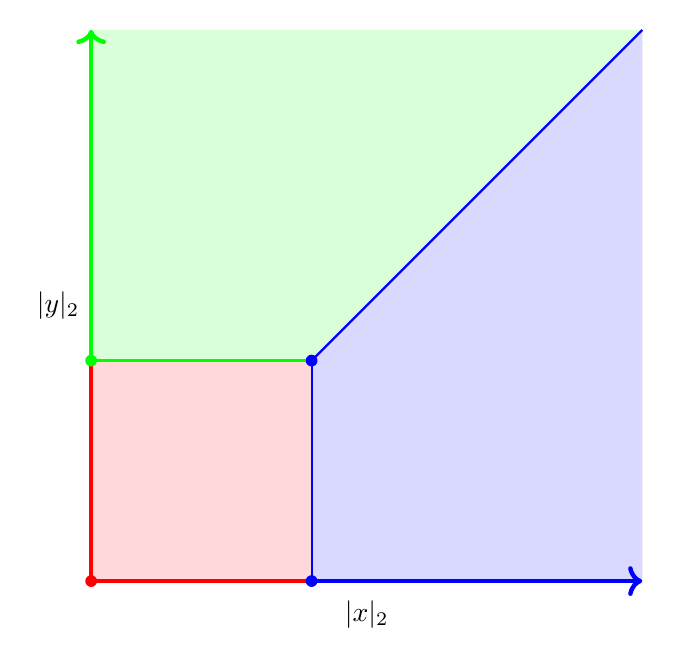
\begin{tikzpicture}[scale=0.7]
\node at (-0.6,5) {$|y|_2$};
\node at (5,-0.6) {$|x|_2$};
\filldraw [thick, fill=red!15] (0,0) rectangle (4,4);
\fill [fill=green!15, even odd rule] (0,4) -- (4,4) -- (10,10) -- (0,10) -- cycle;
\fill [fill=blue!15, even odd rule] (4,0) -- (10,0) -- (10,10) -- (4,4) -- cycle;
\draw[color=red, ultra thick] (0,0) -- (0,4);
\draw[color=red, ultra thick] (0,0) -- (4,0);
\draw[color=green, ultra thick,->] (0,4) -- (0,10);
\draw[color=blue, ultra thick,->] (4,0) -- (10,0);
\draw[color=red, thick] (0,0) -- (4,0);
\draw[color=red, thick] (0,0) -- (0,4);
\draw[color=green, thick] (0,4) -- (0,10);
\draw[color=blue, thick] (4,0) -- (10,0);
\draw[color=blue, thick] (4,4) -- (10,10);
\draw[color=green, thick] (0,4) -- (4,4);
\draw[color=blue,thick] (4,0) -- (4,4);
\node at (4,4) [color=blue,circle,fill,inner sep=1.5pt]{};
\node at (4,0) [color=blue,circle,fill,inner sep=1.5pt]{};
\node at (0,4) [color=green,circle,fill,inner sep=1.5pt]{};
\node at (0,0) [color=red,circle,fill,inner sep=1.5pt]{};
\end{tikzpicture}
\caption*{Coloring of $\Q^2$ in Problem \ref{prob:62}.}
\end{figure}
 Let $(x_r,y_r)$, $(x_b,y_b)$, and $(x_g, y_g)$ be the coordinates of the red, blue, and green vertices of $\Delta$. Then, by a formula  well-known to those who know it well,
\[ 2 \cdot \text{Area}(\Delta) = \pm \left|
\begin{matrix}
 x_b & y_b & 1 \\
x_g & y_g & 1 \\
x_r & y_r & 1
\end{matrix}
\right| = \pm (x_b y_g + x_r y_b + x_g y_r - x_g y_b - x_b y_r - x_r y_g).\]


We claim that $x_b y_g$ has $2$-adic absolute value strictly larger than the other five terms. By definition of the coloring, $|x_b y_g|_2 = |x_b|_{2} |y_g|_{2}\ge 1 \cdot 1 = 1$. Next, we observe that
\[ |x_r|_2 |y_b|_2 \le |x_r|_2 |x_b|_2 < |x_b|_2 \le |x_b|_2 |y_g|_2.  \]
If $y_r=0$, then $|x_g y_r|_2 = 0 < |x_b y_g|_2$; otherwise, 
\[  |x_g|_2 |y_r|_2 < |y_g|_2 |y_r|_2 < |y_g|_2 \le |x_b|_2 |y_g|_2. \]
If $y_b=0$, then $|x_g y_b|_2 = 0 < |x_b y_g|_2$; otherwise,
\[ |x_g|_2 |y_b|_{2} < |y_g|_{2} |y_b|_{2} \le |x_b|_2 |y_g|_{2}. \]
Next,
\[ |x_b|_2 |y_r|_{2} < |x_b|_2  \le |x_b|_2 |y_g|_{2}. \]
Finally, 
\[ |x_r|_2 |y_g|_2 < |y_g|_2 \le |x_b|_2 |y_g|_2.\]
Phew! 

Falling back on ``survival of the greatest,'' we conclude that $|2 \cdot\textrm{Area}(\Delta)|_{2} = |x_b y_g|_{2} \ge 1$, so that $|\textrm{Area}(\Delta)|_2 \ge |2|_2^{-1} > 1$.
\end{sol}


\begin{rmk} Here is a quick sketch of Monsky's proof.\index{Monsky's theorem} We can assume the square we are trying to dissect is $S = [0,1]\times [0,1] \subset \R^2$. 

Color $\Q^2$ as described in Problem \ref{prob:62}. A triangle with vertices from $\Q^2$ will be called a \textsf{rainbow triangle} if each vertex receives a different color. 

Suppose $S$ has been dissected into finitely many triangles. So that we can bring the coloring of $\Q^2$ into the picture, let's suppose that the vertices of all triangles appearing in the dissection have rational coordinates. 

Using a version of Sperner's lemma from combinatorial geometry, along with basic properties of our coloring, Monsky argues that the dissection must contain an \emph{odd} number of rainbow triangles. In particular, there is always at least one rainbow triangle $\Delta$ involved. As we showed above, $|\mathrm{Area}(\Delta)|_2 > 1$. So if we assume there are $n$ triangles involved in the dissection, each with the same area, then $|1/n|_2 > 1$; that is, $n$ is even. 

This is all well and good, but we are interested in arbitrary (real) dissections of $S$, not merely ``rational'' ones. Well, here is the astounding part: The same argument applies in the general case! At first glance this claim doesn't seem to make sense: Our initial coloring was defined in terms of $|\cdot|_2$, and $|\cdot|_2$ has domain $\Q$, not $\R$. It turns out, however, that it is possible to extend $|\cdot|_2$ to an absolute value on $\R$. (This is far from obvious!) With this extension in hand, everything else in the argument goes through with zero change.

A complete proof of Monsky's theorem can be found in \cite[Chapter 22]{AZ18}. The discussion in \cite{AZ18} sidesteps extending $|\cdot|_2$ to an absolute value on $\R$; the reader interested in seeing such an extension constructed can consult \S14 of  \cite{schikhof}.
\end{rmk}

\begin{challenge}[cf. Hales and Straus \cite{HS}] Let $K$ be an infinite field that can be endowed with a nontrivial, non-Archimedean absolute value. Show that it is possible to 3-color the affine plane $K^2$, using all three colors in an interesting way, so that every line receives points of at most two colors.  \textsf{In an interesting way} means that each color is assigned to three non-collinear points. (If we remove ``in an interesting way,'' this can be done for every infinite field. Can you see why?)
\end{challenge}

% \begin{challenge} Let $K$ be a field. It is always possible to 3-color the affine plane $K^2$, using all three colors, in such a way that every line receives points of at most two colors. For instance, color the origin red, then arbitrarily color each line through the origin (minus the origin itself) entirely blue or entirely green, making sure to use both of those colors at least once. 

% To keep the problem interesting, call a 3-coloring of $K^2$ \textsf{nontrivial} if each color is assigned to three non-collinear points. Show that if $K$ admits a nontrivial non-Archimedean absolute value, then $K^2$ admits a nontrivial 3-coloring where each line contains points of at most two colors. (Fields $K$ admitting nontrivial $3$-colorings of this kind are characterized in \cite{HS}.)
% \end{challenge}

\begin{challenge}[Hensel's definition of the $p$-adic integers]\index{$\Z_p$, ring of $p$-adic integers!Hensel's definition} Let $\phi\colon \Z[[T]] \to \prod_{k=1}^{\infty} \Z/p^k$ be the map sending $a_0 + a_1 T + a_2 T^2 + \dots$ to $(a_0 \bmod{p}, a_0 + a_1 p \bmod{p^2}, a_0 + a_1 p + a_2 p^2 \bmod{p^3}, \dots)$. Here the $k$th component of the output is  $a_0 + a_1 p + \dots + a_{k-1} p^{k-1}\bmod p^k$. 
\vspace{-0.12in}
\begin{enumerate} 
    \item[(a)] Check that $\phi$ is a ring homomorphism.
    \item[(b)] Show that $\phi(\Z[[T]]) = \Z_p$. 

{\scriptsize If you squint just right, 
you can see Hensel defining the $p$-adic integers in \cite{hensel13} as the quotient $\Z[[T]]/\ker(\phi)$. This claim must be taken \textsl{cum grano salis}; even the notion of a ``ring''  was still up in the air when \cite{hensel13} was written. Nevertheless, it gets at the essence of Hensel's description.}

\item[(c)] Show that $\ker(\phi) = (T-p)\Z[[T]]$. 
\end{enumerate}
\end{challenge}

\begin{rmk} 
% In addition to anachronistically importing modern concepts (e.g., homomorphisms and their kernels), this take on Hensel's definition disregards Hensel's constructivist requirement that the power series under consideration have coefficients that ``can be calculated as far as desired.''
It seems that neither the definition in \cite{hensel13}, nor Hensel's earlier descriptions in \cite{hensel04, hensel08} (similar but less refined), were viewed by Hensel's contemporaries as entirely rigorous. In his obituary \cite{hasse} for Hensel, Hasse describes the $p$-adic numbers as ``a genuine creation driven by intuition and imagination, which, initially, like every revolutionary idea, was thrown down bluntly and in raw form and which, similar to Leibniz's differential calculus, initially lacked a solid logical foundation.'' Apprehensions about the logical standing of $p$-adic numbers were dispelled only after Kürschák and Ostrowski's papers on valuation theory, which began to appear around the same time as \cite{hensel13}.
\end{rmk}


\let\oldaddcontentsline\addcontentsline
\renewcommand{\addcontentsline}[3]{}
\begin{thebibliography}{11}

\bibitem{AZ18} M. Aigner and {G.\,M}. Ziegler, \emph{Proofs from The Book},
sixth edition, Springer, Berlin, 2018.

\bibitem{cox} R.\,H. Cox, \emph{A proof of the {S}chroeder-{B}ernstein theorem}. Amer. Math. Monthly \textbf{75} (1968), 508.

\bibitem{cuoco91} {A.\,A.} Cuoco,
\emph{Visualizing the $p$-adic integers}. Amer. Math. Monthly \textbf{98} (1991), 355--36.

\bibitem{HS} {A.\,W.} Hales and {E.\,G.} Straus, \emph{Projective colorings}. Pacific J. Math. \textbf{99} (1982), 31--43. 

\bibitem{hasse} H. Hasse, \emph{Kurt Hensel zum Gedächtnis}. J. Reine Angew. Math. \textbf{187} (1949), 1--13.

\bibitem{hensel04} K. Hensel, \emph{Neue Grundlagen der Arithmetik}. J. Reine Angew. Math. \textbf{127} (1904), 51--84.

\bibitem{hensel08} \bysame, \emph{Theorie der algebraischen Zahlen}, {B.\,G.} Teubner, Leipzig and Berlin, 1908.  

\bibitem{hensel13} \bysame, \emph{Zahlentheorie}, {G.\,J.} Göschen, Berlin and Leipzig, 1913.  

\bibitem{holly} {J.\,E.} Holly, 
\emph{Pictures of ultrametric spaces, the $p$-adic numbers, and valued fields}. Amer. Math. Monthly \textbf{108} (2001), 721--728.

\bibitem{katok} S.~Katok, \emph{{$p$}-adic analysis compared with real}, Student Mathematical Library, vol.~37, American Mathematical Society, Providence, RI; Mathematics Advanced Study Semesters, University Park, PA, 2007. 

\bibitem{robert} {A.\,M.} Robert, \emph{A course in p-adic analysis}, Grad. Texts in Math., vol.~198, Springer-Verlag, New York, 2000.   

\bibitem{schikhof} {W.\,H.}~Schikhof, \emph{Ultrametric calculus:  An introduction to $p$-adic analysis}, Cambridge Studies in Advanced Mathematics, vol.~4, Cambridge University Press, Cambridge, 2006.
 \end{thebibliography}
\let\addcontentsline\oldaddcontentsline



\chapter*{Solutions to Set \#6}
\addcontentsline{toc}{chapter}{Solutions to Set \#6}
\markboth{Solutions to Set \#6}{Solutions to Set \#6}
\label{set5sols}


\begin{sol}{prob:68}\index{Cauchy sequence} Suppose $\{x_n\}$ is Cauchy. To prove that $|x_{n+1}-x_n|\to 0$, let $\epsilon > 0$ be given, and select $N \in \Z^{+}$ so that $|x_n-x_m| < \epsilon$ for all positive integers $n,m \ge N$. Then $|x_{n+1}-x_n| < \epsilon$ whenever $n\ge N$. (This direction of the proof does not use that $|\cdot|$ is non-Archimedean.)

Conversely, suppose that $|x_{n+1}-x_n| \to 0$. To prove $\{x_n\}$ is Cauchy, let $\epsilon > 0$, and choose $N \in \Z^{+}$ with $|x_{n+1}-x_n| < \epsilon$ whenever $n\ge N$. If we assume that $n > m \ge N$, the strong triangle inequality yields
\begin{align*} |x_n - x_m| &= |(x_n - x_{n-1}) + (x_{n-1} + x_{n-2}) + \dots + (x_{m+1}-x_m)|
\\&\le \max\{|x_n-x_{n-1}|,\dots,|x_{m+1}-x_m|\} < \epsilon.\end{align*}
The cases where $m > n \ge N$ are interchangeable with these, since $|x_n-x_m| = |x_m-x_n|$. Finally, the inequality $|x_n-x_m| < \epsilon$ is trivial for $n=m$.
\end{sol}


\begin{sol}{prob:70} Let $x_n = 2^{5^n}$. By Euler's theorem, $x_{n+1}-x_n = x_n\cdot (2^{5^{n+1}-5^{n}}-1) = x_n \cdot (2^{\varphi(5^{n+1})}-1) \equiv x_n \cdot 0\equiv 0\pmod{5^{n+1}}$. Thus,  $|x_{n+1}-x_n|_5 \le 5^{-n-1}$, which tends to $0$, and $\{x_n\}$ is a Cauchy sequence by Exercise \ref{prob:68}.
% By Fermat's little theorem, $x_2 = 2^{5^2} = (2^{5})^5 \equiv 2^5 \equiv x_1\pmod{5}$. Suppose that $x_{n+1}\equiv x_n\pmod{5^n}$ for some $n\in \Z^{+}$, and write $x_{n+1} = x_n + 5^n q_n$. Then, working modulo $5^{n+1}$,
% \begin{align*} x_{n+2} \equiv x_{n+1}^5 &\equiv (x_n + 5^n q_n)^{5} \\
% &\equiv x_n^5 + 5^{n+1} x_n^{4} q_n + \sum_{2\le j \le 5} \binom{5}{j} x_n^{5-j} 5^{jn} q_n^{j} \equiv x_n^5 \equiv x_{n+1}. \end{align*}
% (In the last step we use that $jn\ge n+1$ for all $j\ge 2$.) 
\end{sol}

\begin{sol}{prob:68point5} Choose $N \in \Z^{+}$ so that $|x_n-x_m| < 1$ whenever $n, m \ge N$. Then for all $n \ge N$, we have $|x_n-x_N| < 1$, so that \[ |x_n| = |(x_n-x_N) + x_N| \le |x_n-x_N| + |x_N| \le 1 + |x_N|. \]
As a consequence, each $|x_n| \le \max\{|x_1|,|x_2|,\dots,|x_{N-1}|,1+|x_N|\}$.
\end{sol}

\begin{sol}{prob:69} The argument is the same as in calculus. Suppose $\{x_n\}$ is Cauchy and that the subsequence $\{x_{n_k}\}$ converges to $x$. 

Given $\epsilon > 0$, choose $N_1 \in \Z^{+}$ with the property that $|x_k - x_\ell| < \frac{1}{2}\epsilon$ whenever $k,\ell \ge N_1$. Choose $N_2 \in \Z^{+}$ so that $|x_{n_k} - x| < \epsilon$ for all $k \ge N_2$. If $k \ge \max\{N_1, N_2\}$, then
\[ |x_k - x| = |(x_k - x_{n_k}) + (x_{n_k}-x)| \le |x_k - x_{n_k}| + |x_{n_k}-x| < \frac{1}{2}\epsilon + \frac{1}{2}\epsilon = \epsilon. \]
(We use here that $n_k \ge k \ge N_1$.) Hence, $x_k\to x$.
 \end{sol}



\begin{sol}{prob:63} Since $p^{-1} \in \Q_p$, both $\bigcup_{n\ge 0} p^{-n}\Z_p$ and $\Z_p[1/p]$ are contained in $\Q_p$. Both also contain $0$, so we will be done if we show that both contain $\Q_p^{\times}$. 

By Exercise \ref{prob:56}, each $x\in \Q_p^{\times}$ can be written as $\frac{p^v u}{p^{v'} u'}$ for some nonnegative integers $v,v'$ and some $u,u' \in \Z_p^{\times}$. Then $x = p^{v-v'} uu'^{-1} \in p^{v-v'}\Z_p$. Since $p^{v-v'}\Z_p$ is a subset of both $\bigcup_{n\ge 0} p^{-n} \Z_p$ and $\Z_p[1/p]$, it follows that $x$ is contained in both sets.
\end{sol}

\begin{sol}{prob:64}  That $x$ has such a representation is implicit in our solution to Problem \ref{prob:63}. To prove uniqueness, suppose $x=p^{v} u = p^{v'} u'$, with $v,v'\in \Z$ and $u, u' \in \Z_p^{\times}$. Choose $w \in \Z$ large enough that both $v+w$ and $v'+w$ are nonnegative, and apply the already-known uniqueness statement from Problem \ref{prob:56} to $p^w x = p^{v+w} u = p^{v'+w} u'$.
\end{sol}

\begin{sol}{prob:65} Both definitions assign $v_p(0)=\infty$, so it is enough to prove our two definitions of $v_p(x)$ agree for $x \in \Q^{\times}$. Write $x = p^{v} \frac{a}{b}$ where $a$ and $b$ are integers not divisible by $p$. Then $v_p(x)=v$ if we go by the Set \#1 definition. To show $v_p(x)=v$ with our new definition, it suffices to prove that $\frac{a}{b}$ is a unit in $\Z_p$. Thankfully, this is easy: Since $p\nmid ab$, we have both $\frac{a}{b} \in \Z_{(p)} \subset \Z_p$ and $(\frac{a}{b})^{-1} = \frac{b}{a} \in \Z_{(p)} \subset \Z_p$. (See Problem \ref{prob:54} for the containment $\Z_{(p)}\subset \Z_p$.) Thus, $\frac{a}{b} \in \Z_p^{\times}$.

It remains to show that $|\cdot|_p$ is a non-Archimedean absolute value on $\Q_p$. Property (i) in the absolute value definition (see Set \#1) is clear. Property (iii) is straightforward: We can assume $x,y$ are nonzero. Write $x= p^{v_p(x)} u$ and $y=p^{v_p(y)} u'$, where $u, u' \in \Z_p^{\times}$. Then $xy = p^{v_p(x) + v_p(y)} uu'$, and $uu' \in \Z_{p}^{\times}$. Hence, $v_p(xy) = v_p(x)+v_p(y)$, so that $|xy|_{p} = p^{-v_p(x)-v_p(y)}= p^{-v_p(x)} p^{-v_p(y)} = |x|_p|y|_p$. Finally, we turn our attention to the strong triangle inequality: $|x+y|_p \le \max\{|x|_p,|y|_p\}$. For the proof we may assume that $x, y$, and $x+y$ are all nonzero. As above, write $x = p^{v_p(x)} u$ and $y = p^{v_p(y)} u'$. Assuming (as we may) that $v_p(x)\le v_p(y)$, we find that $x+y = p^{v_p(x)} w$ for some $w \in \Z_p$. Furthermore, $w$ is nonzero by our assumption that $x+y\ne 0$. Write $w= p^{v_p(w)} u''$. Then $x+y = p^{v_p(x)+v_p(w)} u''$, and $|x+y|_p = p^{-v_p(x)-v_p(w)} \le p^{-v_p(x)} = \max\{p^{-v_p(x)}, p^{-v_p(y)}\} = \max\{|x|_p, |y|_p\}$.
\end{sol}

\begin{sol}{prob:66} First, we argue that for $x \in \Q_p$:\quad $x \in \Z_p \Longleftrightarrow |x|_p \le 1$. 

We may assume that $x \in \Q_p^{\times}$. Write $x=p^{v_p(x)}u$ where $u \in \Z_{p}^{\times}$. When $v_p(x) \ge 0$, it is clear that $x \in \Z_p$, as both $p^{v_p(x)}$ and $u$ belong to $\Z_p$. On the other hand, Problem \ref{prob:56} gives $v_p(x) \ge 0$ for all nonzero $x \in \Z_p$. Therefore,
\[ x \in \Z_p \Longleftrightarrow v_p(x) \ge 0 \Longleftrightarrow p^{-v_p(x)} \le 1 \Longleftrightarrow |x|_p \le 1,\]
and $\Z_p = \{x\in \Q_p: |x|_p \le 1\}$.

Next, observe that for each nonzero $x \in \Q_p$,
\[ x \in \Z_p^{\times} \Longleftrightarrow v_p(x) = 0 \Longleftrightarrow p^{-v_p(x)}=1 \Longleftrightarrow |x|_p = 1. \]
Hence, $\Z_p^{\times} = \{x \in \Q_p: |x|_p=1\}$. 
\end{sol}


\begin{sol}{prob:67}\index{$\Z_p$, ring of $p$-adic integers!is compact} We address only the part after ``thus''; the earlier claims in the problem are consequences of the Pigeonhole Principle. By construction, $a_{k+1}\equiv a_k \pmod{p^k}$ for every $k$, so that $x:=(a_1\bmod{p},a_2\bmod{p^2},\dots) \in \Z_p$. Furthermore, for each $k$, there are infinitely many $n \in \Z^{+}$ where the mod $p^k$ component of $x_n$ is $a_k\bmod{p^k}$. 

Choose $n_1 \in \Z^{+}$ so that the mod $p$ component of $x_{n_1}$ is $a_1\bmod{p}$. Then choose $n_2 > n_1$ where the mod $p^2$ component of $x_{n_2}$ is $a_2\bmod{p^2}$, then $n_3 > n_2$ where the mod $p^3$ component of $x_{n_3}$ is $a_3\bmod{p^3}$, etc. 

We argue that $x_{n_k} \to x$ in $(\Q_p,|\cdot|_{p})$. Let $k \in \Z^{+}$. By construction, the mod $p^k$ component of $x_{n_k}-x$ vanishes. By the compatibility condition baked into the definition of $\Z_p$, the mod $p$, mod $p^2$, \dots, mod $p^{k-1}$ components also vanish. Therefore (see the solution to Problem \ref{prob:56}), either $x_{n_k}-x=0$ or $x_{n_k}-x = p^{v} u$ for an integer $v \ge k$ and a $u \in \Z_p^{\times}$. In either case, $v_p(x_{n_k}-x) \ge k$, and $|x_{n_k}-x|_p \le p^{-k}$. Since $p^{-k}\to 0$, we conclude that $x_{n_k}\to x$, as required.
\end{sol}

\begin{rmk} Grouchy experts may complain that Problem \ref{prob:67} establishes the \emph{sequential} compactness of $\Z_p$, not \textsf{compactness} with today's accepted meaning in general topology (cf.~\cite{sundstrom}). But those same experts will know that for metric spaces --- such as $\Z_p$ --- the two concepts coincide. So what exactly are they complaining about?

Such grumblers may find the following Extra Exploration more to their tastes.
\end{rmk}

\begin{challenge}[$\Z_p$ is compact, take two]\index{$\Z_p$, ring of $p$-adic integers!is compact}
\vspace{-0.12in}
\begin{enumerate}\item[(a)] A (possibly infinite) number of Ross Program counselors are stationed at points of $\Z_p$. Each counselor is responsible for the campers within a certain positive radius of their position, as measured by $|\cdot|_p$. Presently, all of $\Z_p$ is monitored: each point of $\Z_p$ lies within the assigned radius of some counselor. Show that all but finitely many of the counselors can leave to purchase talent show supplies while $\Z_p$ remains fully monitored (without the need to relocate the remaining counselors).
\item[(b)] What happens if we replace every occurrence of $\Z_p$ by $\Z$? Assume distances are still measured by $|\cdot|_p$ for some prime $p$.
\end{enumerate}
\end{challenge}



\begin{sol}{prob:71}  Let's accept for the time being the identity $\prod_{j\ge 1}\e^{T^j/j}= \frac{1}{1-T}$ in $\Q[[T]]$. 

The series for $\frac{1}{1-T}$ has $T^p$-coefficient (in fact, every coefficient) equal to $1$. To see what the coefficient of $T^p$ looks like on the left side of our identity, we expand
\begin{multline*}\prod_{j=1}^{\infty} \left(1 + \frac{T^j}{j} + \frac{1}{2!} \frac{T^{2j}}{j^2} + \frac{1}{3!}\frac{T^{3j}}{j^3} + \dots\right) \\= \sum_{k\ge 0} T^k \sum_{\substack{e_1+2e_2 + 3e_3 + \dots = k \\ \text{all $e_i \ge 0$}}} \frac{1}{e_1! e_2! e_3!\cdots} \frac{1}{1^{e_1} 2^{e_2} 3^{e_3} \cdots}.  \end{multline*}
All but two of the tuples $e_1,e_2,\dots$ with $e_1+2e_2 + 3e_3 + \dots = p$ have $\frac{1}{e_1! e_2! e_3!\cdots} \frac{1}{1^{e_1} 2^{e_2} 3^{e_3}\cdots} \in \Z_{(p)}$. The two exceptions are (1) the tuple with $e_1=p$ and all other $e_i=0$ and (2) the tuple with $e_p=1$ and all other $e_i=0$, which make respective contributions of $\frac{1}{p!}$ and $\frac{1}{p}$. Equating coefficients of $T^p$ leads to the conclusion that $1 - (\frac{1}{p!} + \frac{1}{p}) \in \Z_{(p)}$, as claimed.

Since $1$ also belongs to the ring $\Z_{(p)}$,  we infer that $\frac{1}{p!} + \frac{1}{p} \in \Z_{(p)}$. But
\[ \left|\frac{1}{p!} + \frac{1}{p}\right|_{p} = \left|\frac{(p-1)!+1}{p!}\right|_p = p |(p-1)!+1|_p. \]
Consequently, $|(p-1)!+1|_p \le 1/p$. This translates to $p\mid (p-1)!+1$, or $(p-1)!\equiv -1\pmod{p}$.\index{Wilson's theorem}

\begin{rmk} It is a little tricky to write down a rigorous proof of the formal identity $\prod_{j\ge 1} \e^{T^j/j} = \frac{1}{1-T}$. We sketch one argument, which, however, involves some `cheating'; specifically we draw  on the theory of complex variables, which is not a prerequisite for the rest of the text.

For each $J \in \Z^{+}$, let $F_J(T) = \prod_{1 \le j \le J} \e^{T^j/j}$ (as a formal power series). Reasoning as in the Remark to Problem \ref{prob:42}, $F_J(z) = \prod_{1\le j \le J} \e^{z^j/j}$ for all complex $z$. As $J\to\infty$, the functions $F_J(z)$ converge uniformly to $\frac{1}{1-z}$ on every compact subset of the open unit disc $|z|<1$. So by Cauchy's integral formula, if we write $F_{J}(T) = \sum_{k \ge 0}a_{k,J} T^k$, then for each fixed $k$,
\[ a_{k,J} = \frac{1}{2\pi \mathrm{i}}\int_{|z|=9/10} F_J(z) z^{-k-1}\,\mathrm{d}z \overset{J\to\infty}{\xrightarrow{\hspace{0.65cm}} } \frac{1}{2\pi i}\int_{|z|=9/10} \frac{1}{1-z} z^{-k-1}\,\mathrm{d}z = 1. \]
(Here we recognized the final integral as the coefficient of $T^{k}$ in $\frac{1}{1-T} = 1 + T +T^2 + \dots$.) Since $a_{k,J}=a_{k,k}$ for all $J\ge k$, we conclude that $a_{k,J}=1$ for all $J\ge k$. In particular: For each fixed $k$, the $k$th coefficient of $F_J(T)$ eventually stabilizes at the $k$th coefficient of $\frac{1}{1-T}$. This is precisely what it means to say that $\prod_{j\ge 1} \e^{T^j/j} = \frac{1}{1-T}$ as formal power series.
\end{rmk} 
\end{sol}



\begin{sol}{prob:72} Write $a^{p-1} = 1 + p q_p(a)$, $b^{p-1} = 1 + p q_p(b)$. Multiplying, $(ab)^{p-1} = 1 + p(q_p(a) q_p(b) + p q_p(a) q_p(b))$, so that
\[ q_p(ab) = \frac{(ab)^{p-1}-1}{p} = q_p(a) + q_p(b) + p q_p(a) q_p(b) \equiv q_p(a) + q_p(b)\!\!\pmod{p}. \]
\end{sol}


\let\oldaddcontentsline\addcontentsline
\renewcommand{\addcontentsline}[3]{}
\begin{thebibliography}{11}

\bibitem{sundstrom}  M.~Raman-Sundström, 
\emph{A pedagogical history of compactness}.
Amer. Math. Monthly \textbf{122} (2015),  619--635.
\end{thebibliography}
\let\addcontentsline\oldaddcontentsline
\chapter*{Solutions to Set \#7}
\addcontentsline{toc}{chapter}{Solutions to Set \#7}
\markboth{Solutions to Set \#7}{Solutions to Set \#7}
\label{set6sols}

\begin{sol}{prob:76} Let $\{x_n\}$ be a Cauchy sequence in $\Z_p$. By Problem \ref{prob:67}, $\{x_n\}$ has a  subsequence $\{x_{n_k}\}$ converging to some $x\in \Z_p$. By Problem \ref{prob:69}, $x_n\to x$.
\end{sol}

\begin{sol}{prob:77} Let $\{x_n\}$ be a Cauchy sequence in $\Q_p$. We know from Exercise \ref{prob:68point5} that $\{|x_n|\}$ is bounded. Hence, if $k$ is sufficiently large, then each $|p^k x_n|\le 1$, i.e., $\{p^k x_n\}$ is a sequence in $\Z_p$. Since $\{x_n\}$ is Cauchy, so is $\{p^k x_n\}$. By Problem \ref{prob:76}, $p^k x_n \to x$ for some $x \in \Z_p$. Then $x_n \to p^{-k} x$.\index{$\Q_p$, field of $p$-adic numbers!is complete}
\end{sol}

\begin{sol}{prob:77andahalf} Let $x_n = 2^{5^n}$. By Problem \ref{prob:70}, $\{x_n\}$ is a Cauchy sequence in $\Z_5$. Invoking Exercise \ref{prob:76}, $x_n \to x$ for some $x\in \Z_p$.

By the product rule for limits, $\lim x_n^5 = (\lim x_n)^5= x^5$. On the other hand, $x_n^{5} = x_{n+1}$, so that $\lim x_n^5 = \lim x_{n+1} = x$. Hence, $x=x^5$.

As shown in the solution to Problem \ref{prob:70}, $x_n = 2^{5^n}\equiv 2^{5^1}\equiv 2\pmod{5}$ for all $n$. Therefore, $|x_n-2|_5 \le \frac15$ for all $n$, and (see Problem \ref{prob:limitabsvalue})
\[ |x-2|_5 = |\lim{(x_n-2)}|_5 = \lim |x_n-2|_5 \le \frac{1}{5}. \]
Thus, $x \equiv 2\pmod{5\Z_5}$. In particular, $x\ne 0$, and $x=x^5$ tells us $1=x^4$. That is, $x$ is a $4$th root of $1$, as claimed.

The only $4$th roots of $1$ belonging to $\Q$ are $1$ and $-1$. Neither is congruent to $2$ modulo $5\Z_5$. Therefore, $x\notin \Q$.
\end{sol}

\begin{sol}{prob:78} Let $x \in \Z_p$. For each $k \in \Z^{+}$, there is an integer $a_k$ with $x\equiv a_k\pmod{p^k\Z_p}$. (If we view $x$ as an infinite tuple, we can take for $a_k$ any integer representing the mod $p^k$ component of $x$; see the solution to Problem \ref{prob:58}.) Then $|a_k-x|_{p} \le p^{-k}$, which tends to $0$ as $k\to\infty$. So $\{a_k\}$ is a sequence of integers converging to $x$.\index{$\Z_p$, ring of $p$-adic integers!has $\Z$ as a dense subset}
\end{sol}

\begin{sol}{prob:79} Let $x \in \Q_p$. Choose $k \in \Z$ with $p^k x \in \Z_p$. By Problem \ref{prob:78}, we can find a sequence of integers $a_k$ converging to $p^k x$. Then $p^{-k} a_k$ is a sequence of rational numbers converging to $x$.\index{$\Q_p$, field of $p$-adic numbers!has $\Q$ as a dense subset}
\end{sol}


\begin{sol}{prob:80} We define a candidate isomorphism $\phi\colon L\to L'$ as follows. Since $K$ is dense in $L$, for each $x \in L$ there is a sequence $\{x_n\}$ in $K$ such that $x_n\to x$ in $L$. Since $\{x_n\}$ converges in $L$, $\{x_n\}$ is Cauchy in $L$. Then $\{x_n\}$ is also Cauchy in $L'$, as each $x_n \in K$ and $|\cdot|$ and $|\cdot|'$ extend the same absolute value on $K$. Since $(L',|\cdot|')$ is complete, $\{x_n\}$ converges in $L'$. We define $\phi(x) = \lim^{(L')} x_n$, where the superscript indicates that the limit is taken in $L'$.

Honor demands we check that $\phi(x)$ depends only on $x$ and not on the particular $\{x_n\}$. Suppose $\{x_n\}$  and $\{\tilde{x}_n\}$ are two sequences in $K$ both converging to $x$ in $L$. Then $x_n-\tilde{x}_n \to 0$ in $L$. As each $x_n -\tilde{x}_n \in K$, and $|\cdot|$ and $|\cdot|'$ extend the same absolute value on $K$, it must be that $x_n-\tilde{x}_n \to 0$ in $L'$. Consequently, $\lim^{(L')} x_n = \lim^{(L')} \tilde{x}_n$. Vindication! 

If $x \in K$, we can compute $\phi(x)$ by taking each $x_n=x$. This shows that $\phi(x) = \lim^{(L')} x = x$. So $\phi$ fixes $K$.

Let $x, y \in L$ and choose sequences $\{x_n\}$, $\{y_n\}$ in $K$ such that $x_n\to x$ in $L$ and $y_n\to y$ in $L$. Then $x_n+y_n \to x+y$ in $L$, and
\[ \phi(x+y) = \sideset{}{^{(L')}}\lim (x_n+y_n) = \sideset{}{^{(L')}}\lim x_n + \sideset{}{^{(L')}}\lim y_n = \phi(x) + \phi(y). \]
Similarly, $\phi(xy) = \phi(x) \phi(y)$, confirming that $\phi$ is a homomorphism.

A homomorphism between fields is always injective. To establish surjectivity, take any $x' \in L'$. Since $K$ is dense in $L'$, there is a sequence $\{x_n\}$ in $K$ converging to $x'$ in $L'$. Since $\{x_n\}$ converges in $L'$, it is Cauchy in $L'$ and hence in $L$ as well. Define $x \in L$ by $x = \lim^{(L)} x_n$. Then $\phi(x) = \lim^{(L')} x_n = x'$. 

Thus far we have shown $\phi$ is an isomorphism. To prove $\phi$ is isometric, let $x \in L$, and consider a sequence $\{x_n\}$ in $K$ converging to $x$ in $L$. Then $\{x_n\}$ converges to $\phi(x)$ in $L'$. Given $\epsilon > 0$, we choose $N \in \Z^{+}$ such that, for all $n\ge N$,
\[ |x_n-x| < \epsilon\quad\text{and}\quad|x_n-\phi(x)|' < \epsilon. \]
Then, for $n\ge N$,
\[ |x| \le |x_n| + \epsilon = |x_n|' + \epsilon < |\phi(x)|' + 2\epsilon, \]
and
\[ |x| \ge |x_n|-\epsilon = |x_n|'-\epsilon \ge |\phi(x)|'-2\epsilon. \]
Hence $|x|$ and $|\phi(x)|'$ are within $2\epsilon$ of each other. Since this holds for each $\epsilon > 0$, it must be that $|x| = |\phi(x)|'$.\index{completion of a valued field!is unique}
% The above arguments establish that $\tilde{\iota}$ is one extension of $\iota$ to an isometric isomorphism between $\Q_p$ and $L$. Suppose $\hat{\iota}$ is any such extension. Let $x\in\Q_p$ and let $x_n$ be a sequence of rational numbers for which $x_n\to x$. 
% Then $x_n-x \to 0$ and, since $\hat{\iota}$ is an isometry and an isomorphism, $\hat{\iota}(x_n)-\hat{\iota}(x) \to 0$. So $\hat{\iota}(x_n)\to  \hat{\iota}(x)$. But $\hat{\iota}(x_n) = \iota(x_n)$ and $\iota(x_n)\to \tilde{\iota}(x)$. Hence, $\hat{\iota}(x) = \tilde{\iota}(x)$. As this holds for each $x \in \Q_p$, we conclude that $\hat{\iota}=\tilde{\iota}$.
\end{sol}

\begin{challenge} Show that the map $\phi$ described above is the \emph{unique} isometric isomorphism from $L$ to $L'$.
\end{challenge}

\begin{rmk} Every valued field $(K,|\cdot|)$ admits a completion (which we have just seen is then unique up to isometric isomorphism). The usual way to show a completion exists is to mimic one of the standard constructions of $\R$ from $\Q$, due to Cantor and M\'eray: Take the ring of Cauchy sequences in $K$ and quotient by the maximal ideal of sequences tending to $0$. For details, see for instance \cite[\S1.3]{katok}. Those with more exotic tastes might enjoy a recent, very different argument by Kionke \cite{kionke}.
\end{rmk}



\begin{sol}{prob:81} Let $s_n = \sum_{k=0}^{n} c_k p^k$. Then $|s_{n+1}-s_n|_p = |c_{n+1} p^{n+1}|_p \le p^{-n-1}$. As $p^{-n-1}\to 0$, the sequence $\{s_n\}$ is Cauchy (see Exercise \ref{prob:68}). By Problem \ref{prob:76}, $s_n$ has a limit in $\Z_p$. This is precisely what it means to say that $\sum_{k=0}^{\infty} c_k p^k$ converges to an element of $\Z_p$.
\end{sol}

\begin{sol}{prob:82} Our selection process guarantees that $x_{k+1}\equiv x \equiv x_k\pmod{p^k\Z_{p}}$ and thus $x_{k+1} \equiv x_k \pmod{p^k}$ (this last congruence holding in $\Z$). It also ensures that $x_k$ is the least nonnegative representative of its residue class mod $p^k$. Therefore, $x_{k+1} \ge x_k$, and $c_k = \frac{1}{p^k} (x_{k+1}-x_k) \ge 0$. Since $x_{k+1} < p^{k+1}$, we also have $c_k < p^{k+1}/p^k = p$. Hence, $c_k \in \{0,1,\dots,p-1\}$. 

Clearly, $x_k\to x$, since $|x_k - x|_p \le p^{-k}$. Moreover,
\[ c_0 + c_1 p + \dots + c_{k-1} p^{k-1} = (x_1-x_0) +(x_2-x_1) + \dots + (x_k-x_1) = x_k-x_0 = x_k \]
for every $k\in \Z^{+}$. Sending $k$ to infinity, $c_0 + c_1 p + c_2 p^2 + \dots = \lim x_k = x$.\index{$\Z_p$, ring of $p$-adic integers!base $p$ expansions of elements}
\end{sol}

% \begin{sol}{prob:83} That there are not two different expansions of $x$ can be established exactly as in the solution to Problem \ref{prob:44}.
% \end{sol}


\begin{challenge} Show that if $p$ is an odd prime, then every $x \in \Z_p$ has a unique representation in the form $\sum_{k=0}^{\infty} d_k p^k$, where the $d_k$ are integers from the interval $(-p/2,p/2)$. For which $x$ is this expansion terminating? For which $x$ is it eventually periodic?
\end{challenge}


\begin{challenge}[Knopfmacher and Knopfmacher \cite{KK}] Prove that every $x \in 1 + p\Z_p$ has a unique product representation $x = (1+p)^{e_1}(1+p^2)^{e_2}(1+ p^3)^{e_3}\cdots$, where $e_1, e_2, e_3,\ldots \in \{0,1,2,\dots,p-1\}$.%\index{infinite product}
\end{challenge}


\begin{challenge}[Pigeons hard at work; Mahler \cite{mahler}] Let $x \in \Z_p$. In this problem we look for prescribed patterns of digits in the base $p$ expansions of the integer multiples of $x$.
\begin{enumerate}
\vspace{-0.12in}
\item[(a)] Let $m, n \in \Z^{+}$. Prove that there are integers $A, B$ with $A\ne 0$, $-p^m \le A  \le p^m$, and $0 \le B < p^n$ satisfying $A x\equiv B\pmod{p^{m+n}\Z_p}$.

{\scriptsize Suggestion. Consider $Ax-B$ mod $p^{m+n}\Z_p$ for $1\le A \le p^m$ and $0 \le B < p^n$. If $0$ mod $p^{m+n}\Z_p$ is represented, you are done. Otherwise, start stuffing pigeons in holes.}

\item[(b)] Taking $m=1$ in (a), show that one of the $2p$ $p$-adic integers $\pm x, \pm 2x, \dots, \pm px$ has infinitely many `$0$' digits in its base $p$ expansion. More generally, for each $m \in \Z^{+}$, one of the $2p^m$ $p$-adic integers $\pm x, \pm 2x, \dots, \pm p^{m} x$ has infinitely many runs of $m$ consecutive zeros in its base $p$ expansion.

\item[(c)] Assume $x$ is an irrational element of $\Z_p$. (That is, $x \in \Z_p \setminus \Z_{(p)}$.) Let $m \in \Z^{+}$, and let $d_0, d_1, d_2, \dots, d_{m-1} \in \{0,1,\dots,p-1\}$. Show that there is a nonzero integer $k$
%, 
%bounded in absolute by value a function of $m$ and $p$ only (meaning, the bound does not depend on $x$ or the particular choice of $d_i$), 
such that the following holds: The digits $d_0, d_1, \dots, d_{m-1}$ appear, in that order, infinitely often in the base $p$ expansion of $kx$.

{\scriptsize The last bit means that if we expand $kx = \sum_{j\ge 0} c_j p^j$, then $c_j = d_0, c_{j+1} = d_1, \dots, c_{j+m-1} = d_{m-1}$ for infinitely many nonnegative integers $j$. For the proof, consider multiples of $k_0 x$, where $k_0 x$ has long runs of zeros as in (b).} 

\item[(d)] Assume $x$ is an irrational element of $\Z_p$. Let $m \in \Z^{+}$. Show that there is a \emph{positive} integer $k'$
%, bounded above by a function of $m$ and $p$ only, 
such that \emph{every} sequence of $m$ base $p$ digits appears infinitely often in the base $p$ expansion of $k' x$.


{\scriptsize Hint. Can you do this with a not-necessarily-positive (but nonzero) $k'$%(still bounded in terms of $m$ and $p$)
? If so, what happens when you replace $k'$ with $-k'$? }
\end{enumerate} 

\end{challenge}

\begin{sol}{prob:84}\index{canonical expansions of elements of $\Q_p$} Start with any $x\in \Q_p$ and select $k\in \Z$ with $p^k x \in \Z_p$. Take the infinite base $p$ expansion of $p^k x$ constructed in Problem \ref{prob:82} and scale by $p^{-k}$ to obtain an expansion of $x$ satisfying (i)--(iii).

If there were two expansions of $x$ possessing properties (i)---(iii), scaling both by the same sufficiently large power of $p$ would produce an element of $\Z_p$ with two different base $p$ expansions.\index{$\Q_p$, field of $p$-adic numbers!base $p$ expansions of elements}
\end{sol}

\begin{sol}{prob:85} The forward direction is clear. Now suppose $x=0$ or $x\in \Q^{+}$ with denominator a power of $p$. Write $x=a/p^k$, where $a$ and $k$ are nonnegative integers. Then the canonical expansion of $x$ is obtained by taking the usual base $p$ expansion of $a$ and scaling by $p^{-k}$; this is obviously terminating.
\end{sol}

\begin{sol}{prob:86}\index{$\Q_p$, field of $p$-adic numbers!element has eventually periodic base $p$ expansion iff rational} We record a simple observation for later use: For each $\ell\in\Z^{+}$, the series $1+p^{\ell}+p^{2\ell} + \dots$ converges to $1/(1-p^{\ell})$ in $(\Q_p,|\cdot|)$. We omit the straightforward proof (compare with Exercise \ref{prob:29}).

Suppose $x$ has an eventually periodic canonical expansion with (not necessarily minimal) period $\ell$. Scaling $x$ by a suitable power of $p$ (which does not affect rationality), we can assume $x= \sum_{k\ge 0} c_k p^k$ where $c_k = c_{k+\ell}$ for all $k\ge k_0$. Then
$x = \sum_{0 \le k < k_0} c_k p^k + \sum_{k \ge k_0} c_k p^k$. Clearly, $\sum_{0 \le k < k_0} c_k p^k \in \Q$. Less trivially,
\begin{align*} \sum_{k \ge k_0} c_k p^k &= \lim_{m\to\infty} \sum_{k_0 \le k 
< k_0+m\ell} c_k p^k \\
&= \lim_{m\to\infty} \sum_{k_0 \le k < k_0+\ell} c_k p^k (1+p^{\ell} + \dots + p^{(m-1)\ell}) \\
&= \sum_{k_0 \le k < k_0+\ell} c_k p^{k} (1+p^{\ell} + p^{2\ell} + \dots)\\
&= \sum_{k_0 \le k < k_0+\ell} c_k \frac{p^k}{1-p^{\ell}} \in \Q.
\end{align*}
Therefore, $x\in \Q$.

Turning to the converse: We have already shown that each $x\in \Z_{(p)}$ has an eventually periodic base $p$ expansion. To obtain an eventually periodic canonical expansion for an arbitrary $x \in \Q$, scale $x$ by $p^k$ to place $p^k x \in \Z_{(p)}$, then rescale by $p^{-k}$.
\end{sol}

\underline{Open problem}: Is the $p$-adic number $\sum_{k=0}^{\infty} k!$ rational for some prime $p$?

\begin{challenge}[Casacuberta \cite{casacuberta}] Show that the $p$-adic number $\sum_{k=0}^{\infty} p^{v_p(k!)}$ has a canonical expansion containing arbitrarily long (but finite) runs of zeros, for every prime $p$. Deduce that $\sum_{k=0}^{\infty} p^{v_p(k!)} \notin \Q$.
\end{challenge}

\begin{challenge}[Dragovich \cite{dragovich}] \underline{Dis}prove: $\sum_{k=0}^{\infty} k!$ converges to the same rational number in $\Q_p$ for all primes $p$.
\end{challenge}


\begin{sol}{prob:87} By Problem \ref{prob:72}, $\sum_{a=1}^{p-1} q_p(a) \equiv q_p((p-1)!) \equiv \frac{(p-1)!^{p-1}-1}{p}\pmod{p}$. So the claimed congruence is equivalent to $\frac{(p-1)!^{p-1}-(p-1)!-2}{p}\equiv 0\pmod{p}$, or $(p-1)!^{p-1} - (p-1)! \equiv 2\pmod{p^2}$. Using Wilson's theorem\index{Wilson's theorem}, write $(p-1)! = -1 + pr$ with $r \in \Z$. Then, working modulo $p^2$, 
\[ (p-1)!^{p-1} = \sum_{j=0}^{p-1} \binom{p-1}{j} (-1)^{p-1-j} (pr)^{j} \equiv 1 + (p-1)(-1)pr \equiv 1 + pr,\] so that $(p-1)!^{p-1} - (p-1)! \equiv (1+pr)-(-1+pr) \equiv 2$, as desired.
\end{sol}

\begin{sol}{prob:98}\index{method of successive approximation} Let us argue that whenever we have a solution to $x^2=2$ in $\Z/7^k$, say $a_k\bmod{7^k}$, we can lift it uniquely --- by the process described --- to a solution $a_{k+1}\bmod{7^{k+1}}$ in $\Z/7^{k+1}$. Expanding, $(a_k + 7^k q)^2 \equiv a_k^2 + 2\cdot 7^{k} a_k q \pmod{7^{k+1}}$. This last expression is congruent to $2$ modulo $7^{k+1}$ precisely when
\[ 2\cdot 7^k a_k q\equiv 2-a_k^2\pmod{7^{k+1}}. \]
By assumption, $7^k \mid 2-a_k^2$. So the preceding congruence is equivalent to
\[ 2a_k q \equiv \frac{2-a_k^2}{7^k} \pmod{7}.\]
Both $2$ and $a_k$ are coprime to $7$. (Since $a_k^2\equiv 2\pmod{7}$,  we cannot have $a_k\equiv 0\pmod{7}$.) Thus, the last displayed congruence uniquely determines the residue class of $q$ modulo $7$. Picking any $q$ from this class and defining $a_{k+1}=a_k + 7^k q$ yields our desired lift. Note that since $q$ is uniquely determined mod $7$, our lift is uniquely determined as a residue class mod $7^{k+1}$.

Assume now that $a_1\bmod{7}, a_2\bmod{7^2}, a_3\bmod{7^3},\dots$ have been determined by the above procedure. Let $x = (a_1\bmod{7}, a_2\bmod{7^2}, a_3\bmod{7^3},\dots)$. Then $x\in \Z_7$ as each $a_{k+1}$ is a lift of $a_k$. By construction, $x^2 = (2\bmod{7},2\bmod{7^2},2\bmod{7^3},\dots) = 2$.

We still need to verify that the canonical expansion of $x$ is as stated. The initial steps of the algorithm, starting with $3\bmod{7}$, are described in the problem statement. We lifted $3\bmod{7}$ to $3+1\cdot 7\bmod{7^2}$, and we lifted \emph{that} to $3+1\cdot 7 + 2\cdot 7^2 \bmod{7^3}$. If we run the algorithm one more round, we arrive at $3+1\cdot 7 + 2\cdot 7^2 + 6\cdot 7^3\bmod{7^4}$ (check this!). We can read off from here that the $7$-adic expansion of $x$ starts as 
$3+1\cdot 7 + 2\cdot 7^2 + 6\cdot 7^3 + \dots$. 

\begin{rmk} Gauss left us in 1855, four decades before Hensel's first publication on the $p$-adic numbers. It is therefore rather remarkable that one finds in his Nachlass (manuscripts left behind at death) the claim that
\[  \sqrt{5} \pmod{11^{\infty}} = 9.0.4.10.4.4.\]
This seems to be Gauss's way of expressing that in $\Z_{11}$,
\[ \sqrt{5} = 4 + 4\cdot 11 + 10 \cdot 11^2 + 4\cdot 11^3 + 0\cdot 11^4 + 9\cdot 11^5+\dots.\]
I owe this historical nugget to math StackExchange user \texttt{user2554}.\footnote{\url{https://math.stackexchange.com/a/4877205}}
\end{rmk}
\end{sol}




\begin{figure}
\centering
\includegraphics[width=0.95\textwidth]{nachlass-BW.pdf}
\caption*{Page from Gauss's Nachlass; originally scanned by the Göttinger Digitalisierungszentrum.}
\end{figure}

\let\oldaddcontentsline\addcontentsline
\renewcommand{\addcontentsline}[3]{}
\begin{thebibliography}{11}

\bibitem{casacuberta} S. Casacuberta, 
\emph{Irrationality of the sum of a $p$-adic series}. Unpublished. \texttt{arXiv:1710.11484 [math.NT]}

\bibitem{dragovich} B. Dragovich,
\emph{On $p$-adic power series}. In: $p$-adic functional analysis (Poznań, 1998), Lecture Notes in Pure and Appl. Math., vol. 207, Dekker, New York, 1999, pp. 65--75. 

\bibitem{katok} S.~Katok, \emph{{$p$}-adic analysis compared with real}, Student Mathematical Library, vol.~37, American Mathematical Society, Providence, RI; Mathematics Advanced Study Semesters, University Park, PA, 2007. 

\bibitem{kionke} S.~Kionke, \emph{Constructing the completion of a field using Quasimorphisms}, 
$p$-Adic Numbers Ultrametric Anal. Appl. \textbf{11} (2019), 335--337.

\bibitem{KK} A. Knopfmacher and J. Knopfmacher, \emph{A binomial product representation for $p$-adic numbers},
Arch. Math. (Basel) \textbf{52} (1989), 333--336.

\bibitem{mahler} K.~Mahler,
\emph{On the digits of the multiples of an irrational $p$-adic number}.
Proc. Cambridge Philos. Soc. 
\textbf{76} (1974), 417--422.

\end{thebibliography}

\let\addcontentsline\oldaddcontentsline

\chapter*{Solutions to Set \#8}
\addcontentsline{toc}{chapter}{Solutions to Set \#8}
\markboth{Solutions to Set \#8}{Solutions to Set \#8}
\label{set7sols}

\begin{sol}{prob:89}\index{convergence of infinite series}\index{$\Q_p$, field of $p$-adic numbers!convergence of series} 
\begin{enumerate}
    \item[(a)] In any complete valued field, a sequence $\{s_n\}$ converges  $\Longleftrightarrow$ $\{s_n\}$ is Cauchy. The forward implication was noted on Set \#6 (for every valued field, not necessarily complete). The backward implication is the definition of completeness.

Let $\sum_{k=1}^{\infty}a_k$ be a series in $K$, a field assumed to be complete with respect to a non-Archimedean absolute value. Put $s_n = \sum_{k=1}^{n} a_k$. Then $\sum_{k=1}^{\infty} a_k$ converges $\Longleftrightarrow$ $\{s_n\}$ converges $\Longleftrightarrow$ $\{s_n\}$ is Cauchy $\Longleftrightarrow$ $s_{n+1}-s_n \to 0$ $\Longleftrightarrow$ $a_{n+1}  \to 0$ $\Longleftrightarrow$ $a_n \to 0$.

\item[(b)] If we assume $\sum_{k=1}^{\infty}a_k$ converges to $s$, then $|s_n| \to |s|$ (see Problem \ref{prob:limitabsvalue}). By the strong inequality, each $|s_n| \le \max\{|a_1|, |a_2|, \dots, |a_n|\} \le \max_{k=1,2,3,\dots}|a_k|$. (That the last max exists is ensured by $|a_k|$ tending to $0$.) Hence, $|s| = \lim |s_n| \le \max_{k=1,2,3,\dots}|a_k|$.\index{strong triangle inequality!extension to infinite series in $\Q_p$}
\end{enumerate}
\end{sol}

\begin{challenge}[convergence of infinite products]\index{convergence of infinite product}\label{pp:infprod} Let $K$ be a field complete with respect to a non-Archimedean absolute value. Let $\{a_k\}$ be a sequence in $K$.
\begin{enumerate}
\vspace{-0.12in}
    \item[(a)] Suppose that $a_k\to 0$. Show that $\prod_{k=1}^{\infty} (1+a_k)$ is a well-defined element of $K$ (meaning that that the partial products have a limit in $K$). Furthermore, $\prod_{k=1}^{\infty} (1+a_k) = 0$ if and only if some $a_k=-1$.
    \item[(b)] Conversely, prove that if $\prod_{k=1}^{\infty}(1+a_k)$ defines a \emph{nonzero} element of $K$, then $a_k\to 0$.
\end{enumerate} 
\end{challenge}

\begin{sol}{prob:90} Let $\sum_{k=1}^{\infty} b_k$ be any rearrangement of $\sum_{k=1}^{\infty} a_k$; say $b_k = a_{\sigma(k)}$ for all $k=1,2,3,\dots$, where $\sigma \in \mathrm{Sym}(\Z^{+})$. Put $s_n = \sum_{k=1}^{n} a_k$ and $t_n = \sum_{k=1}^{n} b_k$. By assumption, $s_n \to s$, while our task is to prove that $t_n \to s$.

Given $\epsilon > 0$, select $N_0 \in \Z^{+}$ with $|a_n| < \epsilon$ whenever $n > N_0$. Then choose $N \in \Z^{+}$ as the maximum of $\sigma^{-1}(1),\dots,\sigma^{-1}(N_0)$. Let us argue that $|t_n-s| < \epsilon$ whenever $n\ge N$.

% Take any $n\ge N$. We start by observing that
% \[ |t_n-s| = |t_n - s_{N_0} + s_{N_0} -s|\le \max\{|t_n - s_{N_0}|, |s_{N_0}-s|\}.\]
% We can write 

Let $n\ge N$. By our choice of $N$, all of $a_1,a_2,\dots,a_{N_0}$ appear among $b_{1},b_2,\dots,b_{N}$, so that 
\[ t_n - s_{N_0} = \sum_{1 \le k \le n} b_k- \sum_{1\le k \le N_0} a_k = \sum_{1 \le k \le n,~\sigma(k) > N_0} a_{\sigma(k)}, \] and
\[ |t_n-s_{N_0}| \le \max\{|a_{\sigma(k)}|: 1 \le k \le n, \sigma(k) > N_0\} < \epsilon. \]
Moreover, \[ |s-s_{N_0}| = \left|\sum_{k > N_0} a_k\right| \le \max_{k > N_0} |a_k| < \epsilon.\] Hence,
\[ |t_n - s| = |(t_n - s_{N_0}) - (s-s_{N_0})| \le \max\{|t_n - s_{N_0}|, |s-s_{N_0}|\} < \epsilon, \]
as desired.
\end{sol}

\begin{sol}{prob:93} Put $s_n= \sum_{k=0}^{n} a_k, t_n = \sum_{k=0}^{n} b_k$, and $u_n = \sum_{k=0}^{n} c_k$. Let $s = \lim s_n$ and $t=\lim t_n$ be the infinite sums of the $a_k$ and $b_k$, respectively. We must show that $u_n \to st$.

Observe that
\[ s_n t_n = \sum_{\substack{0 \le k,\ell \le n \\ k+\ell\le n}} a_k b_\ell + \sum_{\substack{0 \le k, \ell \le n \\ k+\ell > n}} a_k b_\ell 
\]
and that the first of the two right-hand sums satisfies
\[ \sum_{\substack{0 \le k,\ell \le n \\ k+\ell\le n}} a_k b_\ell = \sum_{0 \le r \le n} \sum_{\substack{k+\ell=r \\ k,\ell\ge 0}} a_k b_\ell =  \sum_{0 \le r \le n} \sum_{0 \le k \le r} a_k b_{r-k} = \sum_{0\le r \le n} c_r = u_n. \]
Let $e_n$ be the previously neglected sum, $e_n = \sum_{0 \le k,\ell \le n,~k+\ell>n} a_k b_\ell$. Using $A$ and $B$ to denote upper bounds on $\{|a_k|\}$ and $\{|b_k|\}$ respectively (which certainly exist, since $a_k, b_k \to 0$), we find that
\[ |e_n| \le \max_{0 \le k,\ell \le n, ~k+\ell > n} |a_k b_\ell| \le B\max_{n/2 < k \le n}|a_k|  + A\max_{n/2 < \ell \le n}|b_k|,\]
which tends to $0$. Hence, $e_n\to 0$, and $u_n = s_n t_n - e_n \to st$, as desired.
\end{sol}

\begin{sol}{prob:91} For each fixed $i$, the series $\sum_{j} a_{i,j}$ converges, since $|a_{i,j}| \le \epsilon_j$ and $\epsilon_j\to 0$ as $j\to\infty$. Put $s_i = \sum_{j} a_{i,j}$. Then $\sum_{i} s_i$ also converges, since $|s_i| \le \max\{|a_{i,j}|: j \ge 0\} \le \epsilon_i$, and $\epsilon_i\to 0$ as $i\to\infty$. Thus, we have obtained convergence of the double series $\sum_{i} \sum_{j} a_{i,j}$. A symmetric argument demonstrates the convergence of $\sum_{j} \sum_{i} a_{i,j}$.
\end{sol}


\begin{sol}{prob:92} We start by noting that all of the double series appearing here converge or involve finitely many terms. This follows from Problem \ref{prob:91}. To take one example (the others are similar), $\sum_{i=0}^{N}  \sum_{j} a_{i,j}$ can be rewritten as $\sum_{i}\sum_{j} a_{i,j}\one_{i\le N}$. Since $|a_{i,j}\one_{i\le N}| \le |a_{i,j}|$, the sufficient condition for convergence furnished by Problem \ref{prob:91} is satisfied with the same sequence $\{\epsilon_N\}$.

We can now establish our four inequalities. To attack the first of these, notice that 
\[ \left|\sum_{i} \sum_{j} a_{i,j} - \sum_{i=0}^{N} \sum_{j} a_{i,j}\right| =\left|\sum_{i=N+1}^{\infty} \sum_{j} a_{i,j}\right| \le \max_{i\ge N+1} \left|\sum_{j} a_{i,j}\right|.\]
Each term $a_{i,j}$ appearing in the final sum on $j$ has $i\ge N+1$, and thus $|a_{i,j}| \le \epsilon_{N+1}$. Hence, $|\sum_{j} a_{i,j}|  \le \max_{j} |a_{i,j}| \le \epsilon_{N+1}$ for each $i\ge N+1$, and $\max_{i\ge N+1} |\sum_{j} a_{i,j}| \le \epsilon_{N+1}$. So we have the first inequality.

Analogous reasoning shows that
\[ \left|\sum_{j} \sum_{i} a_{i,j} - \sum_{j} \sum_{i=0}^{N} a_{i,j}\right| = \left|\sum_{j} \sum_{i=N+1}^{\infty} a_{i,j}\right| \le \max_{j} \left|\sum_{i=N+1}^{\infty} a_{i,j}\right| \le \epsilon_{N+1},\]
\[ \left|\sum_{i=0}^{N} \sum_{j} a_{i,j} - \sum_{i=0}^{N}\sum_{j=0}^{N} a_{i,j}\right| = \left|\sum_{i=0}^{N} \sum_{j=N+1}^{\infty} a_{i,j}\right| \le \max_{0\le i \le N} \left|\sum_{j=N+1}^{\infty}a_{i,j}\right| \le \epsilon_{N+1}, \]
and
\[ \left|\sum_{j} \sum_{i=0}^{N} a_{i,j} - \sum_{j=0}^{N}\sum_{i=0}^{N} a_{i,j}\right| = \left|\sum_{j=N+1}^{\infty} \sum_{i=0}^{N} a_{i,j}\right| \le \max_{j\ge N+1} \left|\sum_{i=0}^{N}a_{i,j}\right| \le \epsilon_{N+1}. \]

Now look at the first column of inequalities in the problem statement. These inequalities, in conjunction with the strong triangle inequality, imply that
\[ \left|\sum_{i}\sum_{j} a_{i,j} - \sum_{i=0}^{N} \sum_{j=0}^{N} a_{i,j}\right|  \le \epsilon_{N+1}. \]
Similarly, we obtain from the second column of inequalities that
\[ \left|\sum_{j}\sum_{i} a_{i,j} - \sum_{j=0}^{N} \sum_{i=0}^{N} a_{i,j}\right|  \le \epsilon_{N+1}. \]
Since $\sum_{i=0}^{N} \sum_{j=0}^{N} a_{i,j} = \sum_{j=0}^{N} \sum_{i=0}^{N} a_{i,j}$ (it is always OK to swap  finite sums!), a final application of the strong triangle inequality yields
\[ \left|\sum_{i}\sum_{j} a_{i,j}- \sum_j\sum_i a_{i,j}\right| \le \epsilon_{N+1}.\] Send $N$ to infinity to conclude that $\sum_{i} \sum_{j} a_{i,j} = \sum_{j} \sum_{i} a_{i,j}$.
\end{sol}



\begin{sol}{prob:newbern0} If $p-1 \mid k$, then $n^k\equiv 1\pmod{p}$ for all of $n=1,2,\dots,p-1$, so that $S_k(p) \equiv p-1 \pmod{p}$. Thus, $p\mid S_k(p) + 1 = S_k(p) + \one_{p-1\mid k}$. 

If $p-1\nmid k$, choose an integer $g$ that generates the multiplicative group mod $p$. Working modulo $p$,
\[ g^k S_k(p) = g^k\sum_{0 \le n < p} n^k \equiv \sum_{0 \le n < p} (gn)^k \equiv \sum_{m\bmod{p}} m^k \equiv S_k(p), \]
using that multiplication by $g$ permutes the residue classes modulo $p$. As $g^k\not\equiv 1\pmod{p}$, we infer that $S_k(p)\equiv 0\pmod{p}$. Therefore, $p \mid S_k(p) = S_k(p) + \one_{p-1\mid k}$.
\end{sol}

\begin{sol}{prob:newbern1} By Faulhaber's formula\index{Bernoulli numbers!Faulhaber's formula}\index{Faulhaber's formula}, $\frac{S_k(p)}{p} = \frac{p^{k}}{k+1} + B_k + \sum_{0 < j < k} \binom{k}{j} B_{k-j} \frac{p^j}{j+1}$. Rearranging,
\[ B_k + \frac{\one_{p-1\mid k}}{p} +  \sum_{0 < j < k} \binom{k}{j} B_{k-j} \frac{p^j}{j+1}= \frac{S_k(p)+\one_{p-1\mid k}}{p} - \frac{p^k}{k+1}. \]
It will suffice to argue that both right-hand terms belong to $\Z_{(p)}$.

The first is in $\Z$ (Problem \ref{prob:newbern0}), so certainly also in $\Z_{(p)}$. To handle the second, notice that $p^k \ge 2^k \ge k+1$ for each $k \in \Z^{+}$. Therefore, $v_p(k+1)\le k$, and $v_p(\frac{p^k}{k+1}) = k - v_p(k+1) \ge 0$. That is, $\frac{p^k}{k+1} \in \Z_p$.
\end{sol}

\begin{sol}{prob:newbern2} Suppose the claim is false and let $k$ be the smallest positive integer for which $B_k + p^{-1}\one_{p-1\mid k} \notin \Z_{(p)}$. Let $S$ be the sum on $j$ appearing in Problem \ref{prob:newbern1}, so that $B_k + p^{-1}\one_{p-1\mid k} + S \in \Z_{(p)}$. For use momentarily, we rewrite
\[ S = \sum_{0 < j < k} \binom{k}{j} p B_{k-j} \frac{p^{j-1}}{j+1}.\]

By the minimality of $k$, we have $B_{k-j} + p^{-1}\one_{p-1\mid k-j} \in \Z_{(p)}$ for all $j$ in the range $0 < j < k$. Hence, $pB_{k-j} \in \Z_{(p)}$ for all these $j$. Furthermore, $\frac{p^{j-1}}{j+1} \in \Z_{(p)}$ in this same range of $j$: To see why, note that $p^j \ge 3^j > j+1$, so that  $v_p(j+1) < j$. Since $v_p(j+1)$ is an integer, $v_p(j+1) \le j-1$, and $v_p(\frac{p^{j-1}}{j+1})\ge 0$. It follows that each term in our rewritten expression for $S$ belongs to $\Z_{(p)}$, so that $S$ itself belongs to $\Z_{(p)}$. But if $S \in \Z_{(p)}$ and $B_k + p^{-1}\one_{p-1\mid k} + S \in \Z_{(p)}$, then $B_k + p^{-1}\one_{p-1\mid k} \in \Z_{(p)}$. This contradicts the choice of $k$.
\end{sol}


\begin{sol}{prob:newbern3} This is similar to Problem \ref{prob:newbern2}. Assuming the claim fails, let $k$ be the smallest even positive integer for which $B_{k}+\frac{1}{2}\notin \Z_{(2)}$. From Exercise \ref{prob:newbern1}, $B_{k}+\frac{1}{2} + S\in \Z_{(2)}$, where \[ S=\sum_{0 < j < k} \binom{k}{j} 2B_{k-j}  \frac{2^{j-1}}{j+1}. \]

Let us argue that each term in this expression for $S$ is in $\Z_{(2)}$ (and thus, $S \in \Z_2$). Let $0 < j < k$. If $j$ is odd, then $B_{k-j}=0$ unless $j=k-1$. The $j=k-1$ term of $S$ is $\binom{k}{k-1} 2B_{1} \frac{2^{k-2}}{k} = -2^{k-2}$, which is indeed in $\Z_{(2)}$. (We recalled here that $B_1 = -\frac12$.) If $j$ is even, the minimality of $k$ ensures that $2B_{k-j} \in \Z_{(2)}$. As $\frac{2^{j-1}}{j+1}$ is also in $\Z_{(2)}$ (clear, as $j+1$ is odd), the $j$th term is $2$-integral in the even case as well.

Since $S \in \Z_{(2)}$ and $B_{k}+\frac{1}{2}+S \in \Z_{(2)}$, we are forced to have $B_{k}+\frac{1}{2}\in \Z_{(2)}$. This contradicts the choice of $k$.
\end{sol}


\begin{sol}{prob:97}\index{Bernoulli numbers!Clausen--von Staudt theorem}\index{Clausen--von Staudt theorem} Let $k$ be a positive even integer. From the last two problems we have that for every prime $p$,
\[ B_k +\frac{\one_{p-1\mid k}}{p}  \in \Z_{(p)}. \]
Put
\[ \hat{B}_k := B_k + \sum_{p:~p-1\mid k}\frac{1}{p}.\]
Then for every prime $p$,
\[ \hat{B}_k = \left(B_k + \frac{\one_{p-1\mid k}}{p}\right) +  \sum_{\substack{\ell\text{ prime},~\ell\ne p \\ \ell-1\mid k}} \frac{1}{\ell} \in \Z_{(p)}.  \]
Hence, $\hat{B}_k \in \bigcap_{p} \Z_{(p)} = \Z$.
\end{sol}

\begin{rmk}\index{Bernoulli numbers!distribution of denominators} Let $D_k$ denote the denominator of $B_k$ in lowest terms. The Clausen--von Staudt theorem implies that when $k$ is a positive even integer, $D_k$ is the product of the primes $p$ for which $p-1\mid k$. (So in particular $D_k$ is a multiple of $6$ for all even $k>0$.) It was realized by Erd\H{o}s and Wagstaff \cite{EW} that this characterization of $D_k$ allows one to establish strong statistical results. For example, enlisting methods from analytic number theory --- specifically, the field known as the ``anatomy of integers'' --- they showed that if $D = D_k$ for some positive even $k$, then the limit 
\[ p_D:=
\lim_{x\to\infty} 
\frac{\#\{\text{even positive $n\le x$: $D_n = D$}\}}{\#\{\text{even positive $n\le x$}\}} \]
exists and is positive. That is, any $D$ appearing as a denominator of an even-indexed Bernoulli number actually appears with a well-defined, positive limiting frequency. Furthermore, 
\[ \sum_{D\ge 1} p_D = 1. \]
More recent work on the distribution of the $p_D$ can be found in the article \cite{PW} of Pomerance and Wagstaff; among other things, they re-prove (in stronger form) a theorem of Sunseri that $6$ is the most popular denominator among even-indexed Bernoulli numbers. 
\end{rmk}

\begin{sol}{prob:teichmuller} 
% Put $x_n = u^{p^n}$ for $n=1,2,3,\dots$. Each $x_{n+1}-x_n = x_n (u^{p^{n+1}-p^{n}}-1) = x_n (u^{\varphi(p^{n+1})}-1) \equiv 0\pmod{p^{n+1}}$, implying that $|x_{n+1}-x_n|_p \le p^{-n-1}$. Thus, $\{x_n\}$ is a Cauchy sequence in $\Z_p$.
\index{Teichm\"{u}ller representatives} Since $u$ is a unit in $\Z_p$, it is also a unit modulo every power of $p\Z_p$. Setting $x_n = u^{p^n}$, Euler's theorem yields
\[ x_{n+1} - x_n = x_ n(u^{p^{n+1}-p^n} - 1) = x_n (u^{\varphi(p^{n+1})}-1) \equiv 0 \pmod{p^{n+1}\Z_p}, \]
for each $n=1,2,3,\dots$. (We may appeal to Euler's theorem here since the unit groups of $\Z_p$ mod powers of $p\Z_p$ are ``the same'' as the unit groups of $\Z$ mod powers of $p$, by Problem \ref{prob:justice}.) Hence, $|x_{n+1}-x_n|_p \le p^{-n-1}$ for each $n$, and $\{x_n\}$ is a Cauchy sequence in $\Z_p$.

Let $x = \lim x_n$. Since $\lim x_{n+1} = \lim x_n^{p} = (\lim x_n)^p = x^p$, and $\lim x_{n+1} = \lim x_n = x$, it follows that $x^p=x$.

By Fermat's little theorem, each $x_n = u^{p^n} \equiv u^{p^{n-1}} \equiv \dots \equiv u^p \equiv u\pmod{p\Z_p}$, Therefore, $x\equiv u\pmod{p\Z_p}$ (cf.\ the solution to Problem \ref{prob:77andahalf}), and in particular, $x\ne 0$. Thus, we have shown that $\omega(u):= x$ is a solution to $\omega(u)^{p-1}=1$ with $\omega(u)\equiv u\bmod{p\Z_{p}}$.

To prove $\omega(u)$ is the \emph{unique} $(p-1)$th root of unity congruent to $u\bmod{p\Z_p}$, it is enough to argue that no residue class mod $p\Z_p$ contains two different $(p-1)$th roots of unity. This is easy: The $(p-1)$th roots of unity $\omega(1), \dots, \omega(p-1)$ belong to different residue classes mod $p\Z_{p}$. And these are  all of the $(p-1)$th roots of unity, since the degree $p-1$ polynomial $x^{p-1}-1$ cannot have more than $p-1$ roots in $\Q_p$.
\end{sol}


\begin{sol}{prob:teichmullercalculation} In $\Q_3$, the element $-1$ is a ($3-1$)th root of unity congruent to $2$ modulo $3\Z_3$. Therefore, $\omega(2) = -1$.

Let $p=7$. As seen in the solution to Problem \ref{prob:teichmuller}, $2^{7^{n+1}} \equiv 2^{7^n} \pmod{7^{n+1} \Z_7}$ for each $n \in \Z^{+}$. Hence, for all integers $k\ge 3$,
\[ 2^{7^k} \equiv 2^{7^{k-1}} \equiv \dots \equiv 2^{7^2} \pmod{7^{3}\Z_7}, \]
from which it follows that 
\[ \omega(2)= \lim 2^{7^k}\equiv 2^{7^2}\pmod{7^3\Z_7}. \]
This information is enough to compute $c_0, c_1$, and $c_2$, provided we are willing to get our hands (or computing devices) a little dirty: $2^7 \equiv 128 \pmod{7^3}$, and $2^{7^2} \equiv 128^7 \equiv 324 \pmod{7^3}$. So the base $7$ expansion of $\omega(2)$ begins the same way as that of $324 = 2 + 4\cdot 7 + 6\cdot 7^2$. In other words, the desired digits are $c_0=2, c_1 = 4$, and $c_2 = 6$.
\end{sol}

\begin{sol}{prob:WJteich} We begin with a lemma valid over an arbitrary field of characteristic not equal to $2$.

\begin{lem} Let $F$ be a field of characteristic not equal to $2$. If $\zeta$ is an element of order $3$ in $F^{\times}$, then $1+\zeta$ is an element of order $6$.
\end{lem}

% (In the proof we will only need that $\chara(F) \ne 2$. However, if $\chara(F)=3$, then $F^{\times}$ never has an element of order $3$.)

\begin{proof} By assumption, $\zeta$ is a zero of $T^3-1$ but not $T-1$. Hence, $\zeta$ is a root of $\frac{T^3-1}{T-1} = T^2+T+1 \in F[T]$, and $1+\zeta = -\zeta^2$. Since $\mathrm{char}(F)\ne 2$, the element $-1 \in F^{\times}$ has order $2$, while $\zeta^2$ has order $3$. Since $2$ and $3$ are relatively prime, $1+\zeta = (-1)\cdot \zeta^2$ has order $2\cdot 3=6$.
\end{proof}

Now assume that $u \in \Z$ has order $3$ mod $p$. There are no elements of order $3$ in $\F_2^{\times}$. Hence, $p$ is odd, and we can invoke our lemma to deduce that $1+u$ has order $6$ in $\F_p^{\times}$. In particular, $p\equiv 1\pmod{6}$, as the order of each element in $\F_p^{\times}$ necessarily divides $p-1$; this congruence will be needed shortly.

Continuing, observe that $$ \omega(u)^3 = (\lim_{n\to\infty} u^{p^n})^3 = \lim_{n\to\infty} (u^{3})^{p^n} = \omega(u^3). $$ 
Here $\omega(u^3)$ is the unique $(p-1)$th root of unity congruent to $u^3 \bmod{p\Z_p}$. But $1$ is a $(p-1)$th root of unity, and $1 \equiv u^3 \pmod{p\Z_p}$.  Thus, $1 = \omega(u^3) = \omega(u)^3$. If $\omega(u)=1$, then $u\equiv \omega(u) \equiv 1\pmod{p\Z_p}$, contradicting that $u$ has order $3$ modulo $p$. So $\omega(u)$ is an element of order $3$ in $\Q_p^{\times}$ and, applying the lemma a second time, $1+\omega(u)$ is an element of order $6$. 

In particular, $1+\omega(u)$ is a $(p-1)$th root of unity (since $6\mid p-1$). Furthermore, $1+\omega(u)\equiv 1+u \pmod{p\Z_p}$. Therefore, $1+\omega(u) = \omega(1+u)$.
\end{sol}


\begin{challenge}[$(\Z/p)^{\times}$ is cyclic, revisited, or \emph{sledgehammer swats fly}] For this exercise (only), you are asked to ``forget'' the general result that finite subgroups of multiplicative groups of fields are always cyclic.\footnote{``Please forget everything you have learned at school, because you haven't learned it. Please keep in mind everywhere the corresponding portions of your school work, because you haven't actually forgotten them.'' --- Edmund Landau}
\begin{enumerate}
\vspace{-0.12in}
\item[(a)] Show that the mapping $u \bmod{p}\mapsto \omega(u)$ sets up an isomorphism between $(\Z/p)^{\times}$ and the group $\mu_{p-1}$ of $(p-1)$th roots of unity in $\Q_p$. This map is known as the \textsf{Teichm\"{u}ller lift}.\index{$\Z/p$@$(\Z/p)^{\times}$ is cyclic, proof using Teichm\"{u}ller lift}
\item[(b)] Let $\zeta = \e^{2\pi \mathrm{i}/(p-1)} \in \C$. Explain why the minimal polynomial of $\zeta$ over $\Q$ divides $T^{p-1}-1$. Then deduce from (a) that said minimal polynomial splits over $\Q_p$. Conclude that $\Q(\zeta)$ embeds into $\Q_p$.
\item[(c)] Prove that the image of $\zeta$ under any of the embeddings in (b) generates $\mu_{p-1}$. Hence, $\mu_{p-1}$ and $(\Z/p)^{\times}$ are cyclic.
\end{enumerate}
\vspace{-0.11in}
This unusual argument is due to Matt Baker \cite{baker}.
\end{challenge}


\let\oldaddcontentsline\addcontentsline
\renewcommand{\addcontentsline}[3]{}
\begin{thebibliography}{11}

\bibitem{baker} 
M. Baker, \emph{Primitive roots, discrete logarithms, and p-adic numbers}. URL: \url{https://mattbaker.blog/2013/11/07/primitive-roots-discrete-logarithms-and-the-interplay-between-p-adic-and-complex-numbers/}

\bibitem{EW} P. Erd\H{o}s and S.\,S. Wagstaff, Jr., \emph{The fractional parts of the Bernoulli numbers}. Illinois J. Math. \textbf{24} (1980), 104–-112.

\bibitem{PW} C.~Pomerance and S.\,S. Wagstaff, Jr., \emph{The denominators of the Bernoulli numbers}. Acta Arith. \textbf{209} (2023), 1--15.
\end{thebibliography}
\let\addcontentsline\oldaddcontentsline


% \begin{sol}{prob:94} Recall from Problem \ref{prob:42} that $S_k(n) = \sum_{j=0}^{k} \binom{k}{j} B_{k-j} \frac{n^{j+1}}{j+1}$. Hence,
% $S_k(p^{s}) p^{-s} - B_k = \sum_{j=1}^{k} \binom{k}{j} B_{k-j} \frac{p^{sj}}{j+1}$. Let $M$ be the maximum of $|\binom{k}{j} B_{k-j}\frac{1}{j+1}|_p$ taken over $j=1,2,\dots,k$. Then $|\binom{k}{j} B_{k-j} \frac{p^{sj}}{j+1}|_p \le Mp^{-sj} \le Mp^{-s}$ for each such $j$, and
% \[ |S_k(p^{s}) p^{-s} - B_k|_p \le \max_{1\le j \le k} \left|\binom{k}{j} B_{k-j} \frac{p^{sj}}{j+1}\right|_p \le Mp^{-s}. \]
% Since $Mp^{-s}\to 0$, we conclude that $S_k(p^s) p^{-s} \to B_k$.
% \end{sol}

% \begin{sol}{prob:95} The $n \in I_j$ are the numbers $n = m+ j\cdot p^s$ for $m=0,1,2,\dots,p^{s}-1$. Each $n^k \equiv m^k + jk p^{s} m^{k-1} \pmod{p^{k+1}}$. Summing on $m=0,1,2,\dots,p^{s}-1$ gives $S_k(n) \equiv S_k(p^s) + kj p^s S_{k-1}(p^s) \pmod{p^{s+1}}$, as desired.
% \end{sol}

% \begin{sol}{prob:96} We sum the result of Problem \ref{prob:95} for $j=0,1,\dots,p-1$. Modulo $p^{s+1}$,
% \[ S_k(p^{s+1}) = \sum_{j=0}^{p-1} \sum_{n \in I_j} n^k \equiv pS_k(p^s) + p^s S_{k-1}(p^{s}) \cdot \left(k\sum_{j=0}^{p-1} j\right).  \]
% If $p=2$, then $p\mid k$. (Remember we are assuming that $k$ is even.) If $p$ is odd, then $p\mid \sum_{j=0}^{p-1} j = p\cdot \frac{p-1}{2}$. In either case, $p\mid k\sum_{j=0}^{p-1} j$, and so $p^{s+1} \mid S_{k-1}(p^{s})\cdot (k\sum_{j=0}^{p-1} j)$. Thus, $S_k(p^{s+1}) \equiv p S_k(p^s)\pmod{p^{s+1}}$. 

% As a consequence, \[ \left|\frac{S_k(p^{s+1})}{p^{s+1}} - \frac{S_k(p^s)}{p^s}\right| = \left|\frac{1}{p^{s+1}}\right|_{p} \left|S_k(p^{s+1}) - p S_k(p^s)\right|_p \le p^{s+1} p^{-(s+1)} = 1.\]
% That is, $\frac{S_k(p^{s+1})}{p^{s+1}} - \frac{S_k(p^s)}{p^s} \in \Z_{(p)}$. 
% \end{sol}

\chapter*{Solutions to Set \#9}
\addcontentsline{toc}{chapter}{Solutions to Set \#9}
\markboth{Solutions to Set \#9}{Solutions to Set \#9}
\label{set8sols}

\begin{sol}{prob:99}\index{method of successive approximation} Let $a \in \Z_p^{\times}$. If $a=x^2$ for some $x \in \Q_p$, then $|x|_p^2 = |a|_p = 1$. Therefore, $|x|_p = 1$; in particular, $x \in \Z_p$. Reducing the equation $x^2=a$ modulo the ideal $p\Z_p$ shows that $a\bmod{p\Z_p}$ is a square in $\Z_p/p\Z_p$. Now recall from Exercise \ref{prob:58} that the inclusion of $\Z$ into $\Z_p$ induces an isomorphism between $\Z/p$ and $\Z_p/p\Z_p$ and that this isomorphism identifies $a_1\bmod{p}$ with $a\bmod{p\Z_p}$. Since $a\bmod{p\Z_p}$ is a square in $\Z_p/p\Z_p$, it follows that $a_1\bmod{p}$ is a square in $\Z/p$.

Conversely, suppose $a\in \Z_p^{\times}$ and that $a_1\bmod{p}$ is a square in $\Z/p$. Then $a\bmod{p\Z_p}$ is a square in $\Z_p/p\Z_p$ and we can choose $r_1 \in \Z_p$ with $r_1^2\equiv a\pmod{p\Z_p}$. We construct a $\Z_p$-solution to $x^2=a$ following the iterative procedure of Problem \ref{prob:98}.

Let $k \in \Z^{+}$. Suppose we have a mod $p^k\Z_p$-solution $r_k\bmod{p^k\Z_p}$ to $x^2=a$; we lift this to a mod $p^{k+1}\Z_p$ solution. Expanding, $(r_k + p^k q)^2 \equiv r_k^2 + 2p^k r_k q \pmod{p^{k+1}\Z_p}$. The right-hand side is congruent to $a\bmod{p^{k+1}\Z_p}$ precisely when
\[ 2p^k r_k q \equiv a-r_k^2\pmod{p^{k+1}\Z_p}. \]
By construction, $a-r_k^2 \in p^k\Z_p$, so we can rewrite the last congruence as
\[ 2r_k q \equiv \frac{a-r_k^2}{p^k} \pmod{p\Z_p}.\]
Since $p$ is odd, $2$ is invertible in $\Z_p$. As $r_k^2\equiv a\pmod{p\Z_p}$ and $a\notin p\Z_p$, we have $r_k\notin p\Z_p$. So $r_k$ is invertible in $\Z_p$, and the last displayed congruence is equivalent to 
\[ q \equiv \frac{a-r_k^2}{2 p^k r_k} \bmod{p\Z_p}.\] 
So if we put $r_{k+1} = r_k + p^k\frac{a-r_k^2}{2 p^k r_k} = r_k + \frac{a-r_k^2}{2 r_k}$, then $r_{k+1}\bmod{p^{k+1}\Z_p}$ is a lift of $r_k\bmod{p^k\Z_p}$ to a mod $p^{k+1}\Z_p$ solution of $x^2=a$.

Assume $r_1, r_2, r_3,\dots$ have been determined by the above procedure.
Since $r_{k+1}\bmod{p^{k+1}\Z_p}$ is a lift of $r_k\bmod{p^k\Z_p}$, we have $|r_{k+1}-r_k|_{p} \le p^{-k}$. Thus, $\{r_k\}$ is a Cauchy sequence of elements of $\Z_p$.  Let $x = \lim r_k$, which belongs to $\Z_p$. By construction, $|r_k^2 - a|_p \le p^{-k}$. Thus, $r_k^2 \to a$. Since $r_k^2$ also tends to $x^2$, we conclude that $x^2=a$.
\end{sol}

\begin{rmk} By a small modification of the argument, we can choose our mod $p^k\Z_p$ solutions $r_k$ to all be rational integers. Then their limit $x$ is simply $(r_1\bmod{p}, r_2\bmod{p^2}, r_3\bmod{p^3},\dots) \in \Z_p$.
\end{rmk}

\begin{sol}{prob:100} By Problem \ref{prob:99}, the map $\phi\colon\Z_p^{\times} \to \{\pm 1\}$ that sends $a$ to $\legendre{a_1}{p}$ is a homomorphism with kernel $(\Z_p^{\times})^2$. This homomorphism is onto, as $1$ is sent to $1$ and any $n\in \Z$ with $\legendre{n}{p}=-1$ is sent to $-1$. Therefore, the two cosets of $(\Z_p^{\times})^2$ in $\Z_p^{\times}$ are $\phi^{-1}(1) = (\Z_p^{\times})^2$ and $\phi^{-1}(-1) = n(\Z_p^{\times})^2$, establishing the first claim.\index{$\Z_p$, ring of $p$-adic integers!structure of $\Z_p^{\times}/(\Z_p^{\times})^2$}\index{$\Q_p$, field of $p$-adic numbers!structure of $\Q_p^{\times}/(\Q_p^{\times})^2$}  

Every $x \in \Q_p^{\times}$ has a unique representation in the form $p^v u$ where $v \in \Z$ and $u \in \Z_p^{\times}$. Identifying $p^v u$ with $(v,u)$ sets up an isomorphism $\Q_p^{\times} \cong \Z\times \Z_p^{\times}$, which after quotienting by squares becomes $\Q_p^{\times}/(\Q_p^{\times})^2 \cong \Z/2 \times \Z_p^{\times}/(\Z_p^{\times})^2$. In this last isomorphism, $1, p, n, np$ are sent to the four distinct elements of $\Z/2 \times \Z_p^{\times}/(\Z_p^{\times})^2$. Hence, $1, p, n$, and $np$ are coset representatives for $\Q_p^{\times}/(\Q_p^{\times})^2$.
\end{sol}

\begin{sol}{prob:101} Assume $a \in \Z_2^{\times}$. Then $a$ is a square in $\Q_2$ $\Longleftrightarrow$ $a$ is a square in $\Z_2$ (cf.\ the solution to Problem \ref{prob:99}). 

If $a=x^2$ with $x\in \Z_2$, and $a\in \Z_2^{\times}$, then $x\in \Z_2^{\times}$. Hence, $x\equiv 1,3,5,\text{ or }7\pmod{8\Z_2}$. In each of these cases, $x^2\equiv 1\pmod{8\Z_2}$, and so $a\equiv 1\pmod{8\Z_2}$.

Conversely, suppose that $a\equiv 1\pmod{8\Z_2}$ and write $a=1+8b$. Any square root of $a$ in $\Z_2$ must have the form $1+2y$, for some $y \in \Z_2$. As $(1+2y)^2= a$ $\Longleftrightarrow$ $y^2+y=2b$, it suffices to prove that $y^2+y=2b$ has a solution $y\in \Z_2$. This we do following the method of Problem \ref{prob:99}.

To get started, the residue class $0\bmod{2\Z_2}$ is a mod $2\Z_2$-solution to $y^2+y=2b$. Suppose we have already found a mod $2^k \Z_2$ solution $r_k\bmod{2^k \Z_2}$ to $y^2+y=2b$, where $k \in \Z^{+}$. We proceed to lift this to a mod $2^{k+1}\Z_2$ solution. Expanding, $(r_k+2^{k}q)^2 + (r_k + 2^k q) \equiv r_k^2 + r_k + 2^k q \pmod{2^{k+1}\Z_2}$. The right-hand side is congruent to $2b$ modulo $2^{k+1}\Z_2$ precisely when 
\[ 2^k q \equiv 2b - (r_k^2 + r_k). \]
By construction, $2b-(r_k^2+r_k) \in 2^k \Z_2$, and so this last congruence can be rewritten as
\[ q\equiv \frac{2b-(r_k^2+r_k)}{2^k}\pmod{2\Z_2}. \]
So if we put $r_{k+1} = r_k + 2^k\frac{2b-(r_k^2+r_k)}{2^k} = 2b-r_k^2$, then $r_{k+1}\pmod{2^{k+1}\Z_2}$ is a suitable lift. 

    The rest of the solution is essentially the same as that of Problem \ref{prob:99}.
% Put $r_1=0$; then as shown in the last paragraph, every $x\equiv r_1\pmod{2\Z_2}$ has $x^2\equiv 1 \equiv a\pmod{8\Z_2}$. Let $k \in \Z^{+}$ and suppose every $x$ in the residue class $r_k\bmod{2^k\Z_2}$ satisfies $x^2\equiv a\pmod{2^{k+2}\Z_2}$.
% We describe how to lift $r_k\bmod{2^k\Z_2}$ to a residue class $r_{k+1}\bmod{2^{k+1}\Z_2}$ in such a way  that every $x\equiv r_{k+1} \pmod{2^{k+1}\Z_2}$ has $x^2\equiv a\pmod{2^{k+3}\Z_2}$.


% Expanding, $(r_k + 2^{k+1} q)^2 \equiv r_k^2 + 2^{k+2} r_k q \pmod{2^{k+3}\Z_2}$. The right-hand expression is congruent to $a$ modulo $2^{k+3}$ precisely when 
% \[ 2^{k+2} r_k q \equiv a-r_k^2\pmod{2^{k+3}\Z_2}.\]
% By assumption, $r_k^2-a \in 2^{k+2}\Z_2$. So we can rewrite this last congruence in the form
% \[ r_k q \equiv \frac{a-r_k^2}{2^{k+2}} \pmod{2\Z_2}. \]
% Since $r_k^2\equiv a \equiv 1\pmod{2\Z_2}$, we see that $r_k\notin 2\Z_2$, and thus $r_k \in \Z_2^{\times}$. So we can choose any $q \equiv \frac{a-r_k^2}{2^{k+2} r_k} \pmod{2\Z_2}$. In particular, one suitable lift is $r_{k+1} = r_k + 2^{k+1} \frac{a-r_k^2}{2^{k+2} r_k} = r_k + \frac{a-r_k^2}{2 r_k}$.

% Assume $r_1, r_2, r_3,\dots$ have been determined by the above procedure.
% Since $r_{k+1}\bmod{2^{k+1}\Z_2}$ is a lift of $r_k\bmod{2^k\Z_2}$, we have $|r_{k+1}-r_k|\le 2^{-k-1}$, and so $\{r_k\}$ is a Cauchy sequence in $\Z_2$. Let $x = \lim r_k$. We will show $x^2=a$. By construction, $|r_k^2-a|\le 2^{-k-2}$ and thus $r_k^2\to a$. Since $r_k^2\to x^2$, we conclude that $x^2=a$.
\end{sol}


\begin{sol}{prob:102} By Problem \ref{prob:101}, the homomorphism from $\Z_2^{\times}$ to $(\Z_2/8\Z_2)^{\times}$ sending $a$ to $a\bmod{8\Z_2}$ has kernel $(\Z_2^{\times})^2$. As this homomorphism is easily seen to be surjective, $\Z_2^{\times}/(\Z_2^{\times})^2 \cong (\Z_2/8\Z_2)^{\times} = \{1\bmod{8\Z_2}, 3\bmod{8\Z_2}, 5\bmod{8\Z_2}, 7\bmod{8\Z_2}\}$. Hence, $1, 3, 5$, and $7$ are coset representatives for $(\Z_2/8\Z_2)^{\times}$. Noting that each element of $\Q_2^{\times}$ has a unique representation in the form $2^v u$, with $v \in \Z$ and $u \in \Z_2^{\times}$, we conclude that \[ 1,\enspace 3,\enspace 5,\enspace 7,\enspace 2\cdot 1,\enspace 2\cdot 3,\enspace 2\cdot 5,\enspace  2\cdot 7 \] are coset representatives for $\Q_2^{\times}/(\Q_2^{\times})^2$. (See the solution to Problem \ref{prob:100} for further details on this last step.)
\end{sol}

\begin{challenge} Characterize the elements of $\Z_p$ that can be written as $x^2-y^2$ for $x,y \in \Z_p$. Then do the same for $x^2+y^2$ (harder). For the latter problem, start by showing that every element of $\Z/p$ is a sum of two squares.
\end{challenge}


\begin{sol}{prob:103} Let $a \in \Q_p^{\times}$ and write $a=p^{v} u$ with $u \in \Z_p^{\times}$. If $a=x^n$ for some $x \in \Q_p$, then $n \mid n v_p(x) = v_p(a) = v$. For this to hold for infinitely many $n$ requires $v=0$, so that $a=p^{v}u = u \in \Z_p^{\times}$. This proves the ``$\Longleftarrow$'' implication: If $\sqrt[n]{a} \in \Q_p$ for infinitely many $n$, then $a \in \Z_p^{\times}$.

Now suppose that $a \in \Z_p^{\times}$. It suffices to show that if $\ell$ is any prime not dividing $p(p-1)$, then $a$ is an $\ell$th power in $\Q_p$.

Since $\ell \nmid p-1 = \#(\Z_p/p\Z_p)^{\times}$, the $\ell$th power map is an automorphism of $(\Z_p/p\Z_p)^{\times}$. So we can find an $r_1 \in \Z_p^{\times}$ with $r_1^\ell \equiv a\bmod{p\Z_p}$. We take $r_1\bmod{p\Z_p}$ as our starting point in the method of successive approximation. 

Assume we know a mod $p^k\Z_p$-solution to $x^\ell=a$, say $r_k\bmod{p^k\Z_p}$. We seek a mod $p^{k+1}\Z_p$-solution $r_{k+1}\bmod{p^{k+1}\Z_p}$. Expanding, $(r_k+p^{k}q)^\ell \equiv r_k^\ell + \ell r_k^{\ell-1} p^{k} q \pmod{p^{k+1}\Z_p}$. For the right-hand expression to agree with $a$ mod $p^{k+1}$, we require that $\ell r_k^{\ell-1} p^k q \equiv a-r_k^\ell \pmod{p^{k+1}\Z_p}$, or equivalently
\[ \ell r_k^{\ell-1} q \equiv \frac{a-r_k^{\ell}}{p^k}\pmod{p\Z_p}.\]
Both $r_k$ and $\ell$ belong to $\Z_p^{\times}$. (We use here that $a\in \Z_p^{\times}$ and that $\ell$ is a prime distinct from $p$.) So we can satisfy this congruence with any $q\equiv \frac{a-r_k^{\ell}}{p^k \ell r_k^{\ell-1}}$ modulo $p\Z_p$. In particular, $r_{k+1} = r_k + p^k\frac{a-r_k^{\ell}}{p^k \ell r_k^{\ell-1}} = r_k + \frac{a-r_k^{\ell}}{\ell r_k^{\ell-1}}$ yields a suitable lift.

Assume $r_1,r_2,r_3,\dots$ are chosen according to the above procedure. Each $|r_{k+1}-r_k|\le p^{-k-1}$, so that the $\{r_k\}$ form a Cauchy sequence in $\Z_p$ with a limit $x \in \Z_p$. Since $r_k\to x$, and taking $\ell$th powers preserves limits, $r_k^{\ell}\to x^{\ell}$. On the other hand, each $|r_k^{\ell} -a|\le p^{-k}$, so that $r_k^{\ell}\to a$. Therefore, $x^{\ell}=a$.
\end{sol}

\begin{sol}{prob:104}\index{Liouville's approximation theorem in $\Z_p$} Let $R$ be any commutative ring. If $F(T) \in R[T]$, then $$F(X)-F(Y) \equiv F(Y) - F(Y) \equiv 0 \pmod{(X-Y) R[X,Y]}.$$ So we can write $F(X) - F(Y) = (X-Y) G(X,Y)$ for some $G(X,Y) \in R[X,Y]$.  

If $G(X,Y) \in \Z[X,Y]$ is the polynomial corresponding to our $F(T) \in \Z[T]$, then 
\[ |F(n)-F(\alpha)|_p = |(n-\alpha)G(n,\alpha)|_p \le |n-\alpha|_p. \] 
(To make the last estimate we use that $G$ has $\Z_p$-coefficients and that both $n,\alpha \in \Z_p$.)  This establishes the first claim of the problem.

Since $\alpha$ is a root of $F$, it is clear that $|F(n)-F(\alpha)|_p = |F(n)|_p$.

As $F$ has no integer zeros, $F(n) \ne 0$, so that by the product formula, $|F(n)|_p = |F(n)|_{\infty}^{-1} \prod_{\text{prime }\ell \ne p} |F(n)|_\ell^{-1} \ge |F(n)|_{\infty}^{-1}$.

Write $F(T) = \sum_{k=0}^{d} a_k T^k$. Then
\[ |F(n)|_{\infty} = \left|\sum_{k=0}^{d} a_k n^k\right|_{\infty} \le \left(\sum_{k=0}^{d} |a_k|_{\infty}\right) |n|_{\infty}^{d}.\]  Therefore, $|F(n)|_{\infty}^{-1} \ge c|n|_{\infty}^{-d}$ for $c := (\sum_k |a_k|_{\infty})^{-1}$. (The definition of $c$ makes sense since the $a_k$ are not all zero.) 
\end{sol}

\begin{rmk} When $d\ge 2$ our inequality $|n-\alpha|_p \ge c|n|_{\infty}^{-d}$ can be improved substantially. A theorem of Mahler \cite[Theorem (5,I), p.\ 159]{mahler61} allows us to replace $-d$ with $-1-\epsilon$, for any fixed $\epsilon > 0$. In this new statement, the coefficient $c$ in front of $|n|_{\infty}^{-1-\epsilon}$ is now allowed to depend on both $F$ and $\epsilon$. Mahler's theorem is a $p$-adic variant of a deep result of Klaus Roth, for which Roth was awarded the Fields Medal in 1958.

The exponent $-1-\epsilon$ in Mahler's theorem is  essentially best possible, since approximations to within $|n|_{\infty}^{-1}$ are thick on the ground. Indeed, each $\alpha \in \Z_p$ has a canonical expansion of the form $c_0 + c_1 p + c_2 p^2 + \dots$. If we choose $n=c_0 + c_1 p + \dots + c_{k-1} p^{k-1}$, then $|n-\alpha|_p \le p^{-k} < |n|_{\infty}^{-1}$ (if $n\ne 0$). Provided that $\alpha$ is not a nonnegative integer, varying $k$ yields infinitely many distinct positive integers $n$. By a similar argument, as long as $\alpha$ is not a nonpositive integer, $|n-\alpha|_p < |n|_{\infty}^{-1}$ has infinitely many solutions in negative integers $n$. Therefore, $|n-\alpha|_p < |n|_{\infty}^{-1}$ has infinitely many integer solutions $n$ whenever $\alpha$ is a nonzero element of $\Z_p$. 
\end{rmk}

\begin{challenge} Let $A(T) = \sum_{k=0}^{d} a_k T^k \in \Z_p[T]$. It is easy to prove (and we essentially did this in our solution to Problem \ref{prob:104}) that $|A(x+h) - A(x)|_p \le |h|_p$ whenever $x, h \in \Z_p$. Show that for $x \in \Z_p$ and $h \in p\Z_p$, this bound can be refined to
\[ |A(x+h) - A(x)|_p \le K |h|_p, \]
where $K = \max_{k\ge 0} |k a_k|_p$ is the largest absolute value of any coefficient of $A'(T)$. This is a $p$-adic cousin of the usual mean value theorem (cf.~Robert \cite{robert91}).
\end{challenge}

\begin{sol}{prob:105} That $\alpha := \sum_{k \ge 1} p^{k!} \in \Z_p$ follows from Problem \ref{prob:89}. Suppose for a contradiction that $\alpha$ is a root of the nonconstant polynomial $F(T) \in \Q[T]$. We can assume $F(T)$ is irreducible over $\Q$ and, by clearing denominators, that $F(T) \in \Z[T]$. 

If $F$ has an integer root $n_0$, irreducibility over $\Q$ forces $F$ to be linear with $n_0$ as its only root. In that case, $\alpha = n_0 \in \Z$. But this is absurd: $\alpha$'s canonical expansion is not eventually periodic, so that $\alpha$ is not even rational, let alone a rational integer.

We can therefore apply the result of Exercise \ref{prob:104}. Let $c$ be the constant associated with $F$ in that problem. For each $n$, let $r_n = \sum_{k=1}^{n} p^{k!} \in \Z$. Then $|r_n-\alpha|_p = |\sum_{k > n}p^{k!}|_p \le p^{-(n+1)!}$. Also, $|r_n|_{\infty} \le 2p^{n!}$; here we use that the largest term in the sum defining $r_n$ is $p^{n!}$ and that each term in that sum is at least twice the preceding one. Therefore,
\[ p^{-(n+1)!}\ge |r_n-\alpha|_p \ge c|r_n|_{\infty}^{-d}\ge c \cdot 2^{-d} p^{-d n!}. \]
Rearranging,
\[ p^{n!(d-(n+1))} \ge c \cdot 2^{-d}.\]
But the right-hand side is a positive quantity independent of $n$, while the left-hand side tends to $0$ as $n$ tends to infinity. Contradiction!
\end{sol}

\begin{sol}{prob:106}\index{$\Z_g$, ring of $g$-adic integers!example of $\Z_{10}$}  Given $x\in \Z_{10}$, define the \textsf{$\Z_2$ and $\Z_5$-reductions of $x$} as the first and second components of the image of $x$ under the isomorphism $\Z_{10}\cong \Z_2 \times \Z_5$ described in the solution to Problem \ref{prob:59}. Concretely, if $x=(a_1\bmod{10}, a_2\bmod{10^2}, \dots)$, its $\Z_2$-reduction is $(a_1\bmod{2}, a_2\bmod{2^2}, \dots)$, and its $\Z_5$-reduction is $(a_1\bmod{5}, a_1\bmod{5^2},\dots)$.

Convergence in $\Z_{10}$ can then be defined in terms of convergence in $\Q_2$ and $\Q_5$.  If $\{x_n\}$ is a sequence of elements of $\Z_{10}$, and $x \in \Z_{10}$, we say $x_n\to x$ in $\Z_{10}$ if the $\Z_2$ and $\Z_5$-reductions of the $x_n$ converge to the $\Z_2$ and $\Z_5$-reductions of $x$ (in $\Q_2$ and $\Q_5$).

With this definition of convergence in place, your work on Set \#7 can be adapted to show that every element of $\Z_{10}$ has a unique, convergent $10$-adic expansion $\sum_{k\ge 0} d_k\cdot 10^k$ with each $d_k \in \{0,1,2,\dots,9\}$. (Check this!)

Clearly, $2^{4\cdot 5^n} \to 0$ in $\Z_2$. By Exercise \ref{prob:77andahalf}, $2^{4\cdot 5^n}\to 1$ in $\Z_5$. So the $\Z_{10}$ limit $x$ of $2^{4\cdot 5^n}$ corresponds, under our isomorphism, to $(0,1) \in \Z_2 \times \Z_5$. Write the $10$-adic expansion of $x$ as $\sum_{k\ge 0} d_k \cdot 10^k$ and assume for a contradiction that the sequence $\{d_k\}$ is eventually periodic, say $d_k = d_{k+\ell}$ for all $k\ge k_0$. Working in $\Z_2$, we find that the $\Z_2$-reduction of $x$ is
\begin{multline*} \sum_{0 \le k < k_0} 10^k + \sum_{k_0 \le k < k_0+\ell} d_k \cdot 10^k (1 + 10^{\ell} + 10^{2\ell} + \dots) \\= \sum_{0 \le k < k_0} 10^k + \sum_{k_0 \le k < k_0+\ell} \frac{d_k \cdot 10^k}{1-10^{\ell}}.\end{multline*}
Let $r$ be the rational number defined by the right-hand side. The exact same calculation shows that the $\Z_5$-reduction of $x$ is also $r$. It follows that $x=\sum_{k \ge 0} d_k\cdot 10^k$ is the element of $\Z_{10}$ corresponding under our isomorphism to $(r,r) \in \Z_2\times \Z_5$. But we saw already that $x$ corresponds to $(0,1)$. Contradiction! 
\end{sol}

\begin{challenge} Say that the infinite sequence of decimal digits $d_0$, $d_1$, $d_2$, $d_3, \dots$ is \textsf{self-squaring} if, for every $k \in \Z^{+}$, \[ (d_0 + d_1 \cdot 10 + \dots + d_{k-1} \cdot 10^{k-1})^2 \equiv d_0 + d_1 \cdot 10 + \dots + d_{k-1}\cdot 10^{k-1} \pmod{10^k}. \]
For example, the two sequences $0,0,0,0,\dots$ (all zeros) and $1,0,0,0,\dots$ (all zeros past the first term) are trivially self-squaring.
\begin{enumerate}
\vspace{-0.12in}
\item[(a)] Prove that there is a unique self-squaring sequence starting with $d_0=6$.
\item[(b)] Show that the sequence in (a) begins 6, 7, 3, 9, 0, 1, 7, 8, 7, 1. (As a spot check, $76^2 = 57\underline{76}$, while $109376^2= 11963\underline{109376}$.)
\item[(c)] How many self-squaring sequences are there?
\end{enumerate}
\end{challenge}




\begin{challenge}[Shapiro and Shapiro \cite{SS}]\label{challenge:SS} Let $a_1, a_2, a_3, \dots$ be an arbitrary sequence of positive integers. Show that for every $g\in\Z^{+}$, the sequence $a_1, a_1^{a_2}, a_1^{a_2^{a_3}}, \dots$ stabilizes modulo $g$. Deduce that for each $g>1$, this same sequence converges in $\Z_g$. (Define convergence in $\Z_g$ by mimicking what we did for $\Z_{10}$ above.) 
\end{challenge}

\begin{challenge}[continuation]
Let $a$ be a positive integer not divisible by $10$. By \pp~\ref{challenge:SS},  for each $k\in \Z^{+}$ the residue class mod $10^k$ of $a, a^a, a^{a^{a}},\dots$ eventually stabilizes. Let $x_k$ be the least nonnegative integer in the limiting residue class mod $10^k$, so that $0 \le x_k < 10^k$. 
%(Thus, $(x_1\bmod{10}, x_2\bmod{10^2}, x_3\bmod{10^3},\dots)\in \Z_{10}$.)
\begin{enumerate}
\vspace{-0.12in}
\item[(a)] Show that for each $k\ge 2$, we have $a^{x_k} \equiv x_k\pmod{10^k}$.
\item[(b)] Let $a=73$. Compute $x_{33}$, by hook or by crook, and thereby show that
\[ 73^{990485815519399724778909194186633} = \dots990485815519399724778909194186633.\]
\end{enumerate}
\vspace{-0.10in}
For more on this theme, see the papers of Jim\'enez Urroz \& Yebra \cite{UY} and Germain~ \cite{germain}.
\end{challenge}

\begin{sol}{prob:107} The first equivalence is immediate from Problem \ref{prob:89}. 

Turning to the second: If $x \in \Z_p$, then $|a_n x^n|_p \le |a_n|_p$ for all $n$. So if $|a_n|_p\to 0$, then $\sum_{n\ge 0} a_n x^n$ converges for all $x \in \Z_p$.

Conversely, suppose that $\sum_{n\ge 0} a_n x^n$ converges for all $x \in \Z_p$. Then $\sum_{n\ge 0} a_n$ converges (the case $x=1$), so that $|a_n|_p  \to 0$.
\end{sol}

\begin{challenge} Check that the Strassmann series form a subring of $\Q_p[[T]]$. This ring is commonly denoted $\Q_p\langle T\rangle$\index{$\Q_p\langle T\rangle$, ring of Strassmann series (Tate algebra)}\index{Strassmann series!form a subring of $\Q_p[[T]]$} and referred to as the \textsf{Tate algebra in one variable over $\Q_p$}. 
Show that for each $z \in \Z_p$, the evaluation map $\mathrm{eval}_z\colon \Q_p\langle T\rangle \to \Q_p$ sending $F(T)$ to $F(z)$ is a ring homomorphism.
\end{challenge}

\begin{sol}{prob:108} Since $F(T)$ is a Strassmann series, its coefficients $a_n$ tend to $0$. In particular, $\{|a_n|_p\}$ is bounded, and $p^k F(T) \in \Z_p[[T]]$ for a certain integer $k$. Since $F$ and $p^k F$ have the same zeros, we can (and will) assume that $F(T) \in \Z_p[[T]]$ to start with.

Let $m$ be the smallest nonnegative integer for which $a_m\ne 0$ and let $\delta = |a_m|_p$. Note that $\delta \le 1$, since $F(T) \in \Z_p[[T]]$. If $0 < |x|_p < \delta$, then
\[ \bigg|\sum_{n > m} a_n x^n\bigg|_p \le \max_{n > m}{|a_n x^n|_p} \le |x|_p^{m+1} < \delta |x|_p^{m} = |a_m x^m|_p = \bigg|\sum_{n=0}^{m} a_n x^n\bigg|_p.\]
Therefore,
\[ |F(x)|_p = \left|\sum_{n=0}^{m} a_n x^n + \sum_{n > m} a_n x^n\right|_p \ge \bigg|\sum_{n=0}^{m} a_n x^n\bigg|_p - \bigg|\sum_{n>m} a_n x^n\bigg|_p > 0, \]
so that $F(x)\ne 0$.

As a consequence, if $F(T)$ is Strassmann and not the zero series in $\Q_p[[T]]$, then $F(p^m)$ is nonzero for all sufficiently large $m$ (specifically, for any $m$ with $p^{-m} < \delta$). Hence, a Strassmann series that vanishes everywhere on $\Z_p$ must be the zero series.
\end{sol}

\begin{sol}{prob:109} Substituting and applying the binomial theorem, we find that whenever $x,x_0 \in \Z_p$,
\[ F(x+x_0) =  \sum_{k\ge 0} a_k(x+x_0)^k = \sum_{k \ge 0} \sum_{j \ge 0} \mathbf{1}_{k\ge j} a_k \binom{k}{j} x^j x_0^{k-j}. \]
We would like to reverse the order of summation. To justify this we appeal to the criterion of Exercise \ref{prob:92}. Put $u_{k,j} = \mathbf{1}_{k\ge j} a_k \binom{k}{j} x^j x_0^{k-j}$. If we set $\epsilon_{N} = \max_{k\ge N} |a_k|_p$, then $|u_{k,j}|_p \le \epsilon_{N}$ whenever $k\ge N$ or $j \ge N$. Since $F(T)$ is a Strassmann series, $\epsilon_N\to 0$ as $N\to\infty$, and so the conditions of Exercise \ref{prob:92} are satisfied. Therefore,
\begin{align*} F(x+x_0) &= \sum_{k} \sum_{j} u_{k,j} = \sum_{j} \sum_{k} u_{k,j} = \sum_{j\ge 0} \left(\sum_{k\ge j} a_k \binom{k}{j} x_0^{k-j}\right)x^j.
\end{align*}
Here the coefficient of $x^j$ is precisely the claimed coefficient $b_j$.

Since $\sum_{j\ge 0} b_j x^j$ converges for all $x \in \Z_p$ (to $F(x+x_0)$), $\sum_{j\ge 0} b_j T^j$ is a Strassmann series.
\end{sol}

\begin{sol}{prob:110}\index{Strassmann series!if nonzero has finitely many zeros in $\Z_p$} Let $F(T)$ be a Strassmann series, $F(T) \ne 0$. Suppose for a contradiction that $F$ has an infinite number of zeros in $\Z_p$, and let $x_1, x_2, x_3,\dots$ be a sequence of distinct zeros. As $\Z_p$ is compact (Problem \ref{prob:zpcompact}), there is an $x_0 \in \Z_p$ such that some subsequence of $\{x_n\}$ converges to $x_0$.

Problem \ref{prob:109} describes how to construct a Strassmann series $G(T)$ with $G(x) = F(x+x_0)$ for every $x \in \Z_p$. By the choice of $x_0$, every open disc centered at $x_0$ contains infinitely many zeros of $F$. Hence, every open disc centered at $0$ contains infinitely many zeros of $G$. This contradicts Exercise \ref{prob:108} unless $G(T)=0$ in $\Q_p[[T]]$. But that's impossible: If $G(T) = 0$, then $F(x) = G(x-x_0)=0$ for all $x \in \Z_p$. But a nonzero Strassmann series such as $F(T)$ cannot vanish on all of $\Z_p$ (Exercise \ref{prob:109}).
\end{sol}



\begin{challenge}\label{pp:entireproduct} We assume familiarity with  infinite products, as defined in \pp~\ref{pp:infprod}. Let $c_1, c_2, c_3, \dots$ be a sequence of elements of $\Q_p$ tending to $0$. By \pp~\ref{pp:infprod}, the infinite product $\prod_{j=1}^{\infty} (1-c_j x)$ determines a well-defined element of $\Q_p$ for all $x \in \Q_p$. Write down a power series $F(T) \in \Q_p[[T]]$ with the property that $F(x) = \prod_{j=1}^{\infty} (1-c_j x)$ for all $x \in \Q_p$. 
\end{challenge}

\begin{challenge}[continuation; Sch\"{o}be {\cite[p.\ 38]{schoebe}}]\label{pp:noliouville} Let $e_1, e_2, e_3, \dots$ be a sequence of positive integers. For each $x \in \Q_p$, let $A(x) = \prod_{j=1}^{\infty} (1-(p^j x)^{p-1})^{e_j}$. 
\begin{enumerate}
\vspace{-0.12in}
\item[(a)] Prove that $A(x)$ is a well-defined function from $\Q_p$ to $\Q_p$ and that $A(x)$ can be represented by an everywhere convergent power series with $\Q_p$-coefficients.
\item[(b)] Show that $|A(x)|_p = 1$ if $x \in \Z_p$.
\item[(c)] Suppose $|x|_p = p^{r}$, where $r$ is a positive integer. Show that $|A(x)|_p \le p^{-e_r} \prod_{j=1}^{r-1} p^{(r-j)(p-1) e_j}$.
\item[(d)] Describe a method of choosing $e_1, e_2, e_3, \dots$ that guarantees $|A(x)|_p \le |x|_p^{-1}$ whenever $x \in \Q_p\setminus \Z_p$.
\item[(e)]  Deduce from (a)--(d) that there is an  power series over $\Q_p$ that converges everywhere and induces a bounded but nonconstant function from $\Q_p$ to $\Q_p$. For those who have taken a complex variables course: Explain how this suggests $\Q_p$ is more analogous to $\R$ than to $\C$.
\end{enumerate}
\end{challenge}


\begin{sol}{prob:111}\index{Bernoulli numbers!associated characterization of Wilson primes} When $p=2$, neither statement holds. So assume $p$ is odd.

By Problem \ref{prob:87}, $\frac{(p-1)!+1}{p} \equiv \sum_{a=1}^{p-1} q_p(a)\pmod{p}$. So it suffices to show that $\sum_{a=1}^{p-1} q_p(a) - (B_{p-1}+\frac{1}{p}-1) \in p \Z_{(p)}$.

By Faulhaber's formula\index{Bernoulli numbers!Faulhaber's formula}\index{Faulhaber's formula}, 
\[ \sum_{a=1}^{p-1} q_p(a) = \frac{S_{p-1}(p)}{p} -\frac{p-1}{p} = B_{p-1} + \frac{1}{p} -1 + \sum_{j=1}^{p-1} \binom{p-1}{j} B_{p-1-j} \frac{p^{j}}{j+1}.\]
For each $j=1,2,3,\dots,p-1$, the Bernoulli number $B_{p-1-j} \in \Z_{(p)}$; this is clear for $j=p-1$ (recall that $B_0=1$) and for $j < p-1$ it follows from Exercise \ref{prob:newbern2}. In this same range of $j$, we have $p^j \ge 3^j > j+1$. Thus, $v_p(j+1) < j$, and $v_p(\frac{p^j}{j+1}) = j - v_p(j+1) > 0$.  Consequently, each term in our sum on $j$ belongs to $p\Z_{(p)}$, implying that the sum itself belongs to $p\Z_{(p)}$. But that sum is precisely $\sum_{a=1}^{p-1} q_p(a) - (B_{p-1}+\frac{1}{p}-1)$.
\end{sol}

\begin{sol}{prob:WJfermat}\index{Teichm\"{u}ller representatives}   By Problem \ref{prob:WJteich} and its solution, $p\equiv 1\pmod{6}$ and $\omega(1+u) = 1 + \omega(u)$. Write $v=\omega(u) + p^k q$, where $q \in \Z_p$. Since $p$ is odd and $p \mid \binom{p}{k}$ for all $k$ between $0$ and $p$,
\begin{align*}
  v^p = (\omega(u)+p^k q)^p &\equiv \omega(u)^{p} + \omega(u)^{p-1} p^{k+1} q \pmod{p^{2k+1}p\Z_p} \\
      &\equiv \omega(u) + p^{k+1} q \pmod{p^{2k+1} p\Z_p}. 
\end{align*} 
On the other hand, $1+v = 1 + \omega(u) + p^k q = \omega(u+1) + p^k q$, and (by analogous reasoning to what is displayed above)
\[ (1+v)^p \equiv \omega(u+1) + p^{k+1} q \pmod{p^{2k+1} p\Z_p}. \]
Using once more that $1+\omega(u) = \omega(u+1)$, we deduce that $(1+v)^p \equiv 1 + v^p \pmod{p^{2k+1}\Z_p}$. Since both $(1+v)^p$ and $1+v^p$ lie in $\Z$, this last congruence in fact holds modulo $(p^{2k+1} \Z_p) \cap \Z = p^{2k+1} \Z$. 

Let $p=7$. In the course of solving Problem \ref{prob:teichmullercalculation}, we computed that $\omega(2) \equiv 324 \pmod{7^3 \Z_7}$. Taking $v=324$ and $k=3$ in the result of the last paragraph ``explains'' the given example.
\end{sol}


\let\oldaddcontentsline\addcontentsline
\renewcommand{\addcontentsline}[3]{}
\begin{thebibliography}{11}

\bibitem{germain} J. Germain, \emph{
On the equation $a^x \equiv x\pmod{b}$}. 
Integers \textbf{9} (2009), A47, 629--638.


\bibitem{UY} J. Jiménez Urroz and {J.\,L.\,A.} Yebra, \emph{On the equation $a^x\equiv x\pmod{b^n}$}. J. Integer Seq. \textbf{12} (2009), Article 09.8.8, 8 pp.



\bibitem{mahler61} K. Mahler, \emph{Lectures on Diophantine approximations. Part I: $g$-adic numbers and {R}oth's theorem}, Notre Dame Mathematical Lectures, vol. 7, University of Notre Dame Press, Notre Dame, 1961.

\bibitem{robert91} A. Robert, \emph{A note on the numerators of the Bernoulli numbers}. Exposition. Math. \textbf{9} (1991), 189--191. 

\bibitem{schoebe} W. Schöbe, \emph{Beiträge zur Funktionentheorie in nichtarchimedisch bewerteten Körpern}. Münster: Diss. Math. Univ. Münster, Universitas-Archiv \textbf{42}, Math. Abteilung Nr. 2 (1930), 61 pp.


\bibitem{SS} {D.\,B.} Shapiro and {S.\,D.} Shapiro, \emph{Iterated exponents in number theory}. Integers \textbf{7} (2007), A23, 19 pp.

\end{thebibliography}
\let\addcontentsline\oldaddcontentsline
\chapter*{Solutions to Set \#10}
\addcontentsline{toc}{chapter}{Solutions to Set \#10}
\markboth{Solutions to Set \#10}{Solutions to Set \#10}
\label{set9sols}

\begin{sol}{prob:F12convergence} 
We begin by establishing some useful arithmetic properties of the generalized binomial coefficients $\binom{\frac{1}{2}}{k}$ for nonnegative integers $k$.

Fix $k$. Let $\ell$ be an odd prime, and let $A$ be a nonnegative integer with $\frac{1}{2} \equiv A \pmod{\ell^{v_\ell(k!)}\Z_\ell}$; e.g., $A =\frac{1}{2} (\ell^{v_\ell(k!)}+1)$. Since $\binom{A}{k} \in \Z$,
\[ \ell^{v_\ell(k!)} \mid k! \mid \binom{A}{k} k! = A(A-1)(A-2) \cdots (A-(k-1)), \]
where the divisibility relations are being asserted in the ring $\Z$. Naturally, these same relations also hold in $\Z_{\ell}$, so that working in $\Z_{\ell}$ modulo $\ell^{v_\ell(k!)}\Z_{\ell}$,
\[ \frac{1}{2}\left(\frac{1}{2}-1\right) \cdots \left(\frac{1}{2}-(k-1)\right) \equiv A(A-1)\cdots (A-(k-1)) \equiv 0. \]
It follows that $v_\ell(\frac{1}{2}(\frac{1}{2}-1) \cdots (\frac{1}{2}-(k-1))) \ge v_\ell(k!)$, so that $v_\ell(\binom{\frac{1}{2}}{k})  \ge 0$. % In $\Z_p$, the elements $k!$ and $p^{v_p(k!)}$ are associates. So % let $x_n = \frac{1}{2}(\ell^n+1)$; the $x_n$ are positive integers converging to $\frac12$ in $\Q_\ell$. By the limit laws established in Problem \ref{prob:calclimits}, for every nonnegative integer $k$,
% \begin{align*} \lim_{n\to\infty} \binom{x_n}{k} &= \lim_{n\to\infty} \frac{x_n(x_n-1)\cdots(x_n-(k-1))}{k!}\\ &= \frac{\frac{1}{2}(\frac{1}{2}-1)\cdots(\frac{1}{2}-(k-1))}{k!} =\binom{\frac{1}{2}}{k}. \end{align*}
% Therefore, $|\binom{\frac{1}{2}}{k}|_\ell = \lim |\binom{x_n}{k}|_\ell \le 1$ (since each $\binom{x_n}{k} \in \Z$, and $\Z\subset \Z_\ell$). 
As this holds for all odd primes $\ell$, the rational number $\binom{\frac{1}{2}}{k}$ has denominator a power of $2$.

To determine which power of $2$, we look $2$-adically. Expanding out, $$\binom{\frac{1}{2}}{k} = \frac{1\cdot (1-2)\cdot (1-2\cdot 2) \cdots (1-2(k-1))}{2^k k!}.$$  
The numerator on the right is odd, and so the power of $2$ in the denominator of $\binom{\frac{1}{2}}{k}$ is $2^{k+v_2(k!)}$. 

Collecting what we know so far: $\binom{\frac12}{k}$ is a rational number with denominator $2^{k+v_2(k!)}$.

We are now well-positioned to decide when $B_{\frac{1}{2}}(x)$ converges --- equivalently, when $|\binom{\frac{1}{2}}{k} x^k|_p \to 0$ (as $k\to\infty$). For use momentarily, we recall that $v_2(k!) \le k$, so that $k+v_2(k!) \le 2k$. 


Suppose $p$ is odd. Then $|\binom{\frac12}{k}|_p\le 1$, and $|\binom{\frac{1}{2}}{k} x^k|_p \le |x|_p^{k}$. If $|x|_p \le 1/p$, then $|x|_p^{k} \to 0$ as $k\to\infty$. Thus, $B_{\frac{1}{2}}(x)$ converges for these $x$.

Suppose instead that $p=2$. If $x \in \Q_2$, then $|\binom{\frac{1}{2}}{k} x^k|_2 = 2^{k+v_2(k!)} |x|_2^{k}\le 2^{2k} |x|_2^{k}$. This last expression tends to $0$ if $|x|_2 \le 1/2^{3}$. 

These conditions on $x$ turn out to be   necessary for convergence. 

\begin{lem} Let $F(T) \in \Q_p[[T]]$. If $F(x_0)$ converges ($x_0 \in \Q_p$), then $F(x)$ converges for all $x \in \Q_p$ with $|x|_p \le |x_0|_p$.
\end{lem}
\begin{proof} Write $F(T) = \sum_{k\ge 0} a_k T^k$. If $|a_k x_0^k|_p\to 0$, and $|x|_p \le |x_0|_p$, then  $|a_k x^k|_p\to 0$.
\end{proof}

Seeking a contradiction, suppose $p$ is odd and that $B_{\frac12}(x_0)$ converges for a value of $x_0$ with $|x_0|_p > 1/p$. Then $|x_0|_p \ge 1$. Invoking the lemma, $B_{\frac12}(x)$ converges whenever $|x|_p\le 1$, i.e., on all of $\Z_p$. But whenever $B_{\frac12}(x)$ converges, it converges to a square root of $1+x$. We infer that that every element of $\Z_p$ has a square root in $\Q_p$ --- absurd! 

Similarly, if $B_{\frac{1}{2}}(x)$ converges for an $x_0\in \Q_2$ with $|x_0|_2 > 1/2^3$, then it converges whenever $|x|_2 \le 1/2^2$. But then $B_{\frac{1}{2}}(4)$ converges to a square root of $5$ in $\Q_2$, whereas $5 \notin (\Q_2^{\times})^2$!
\end{sol}

\begin{challenge}\label{pp:binomial0}\mbox{ }
\vspace{-0.12in} Establish the following claims.
\begin{enumerate}
    \item[(a)] If $x \in \Z_p$ and $k$ is a nonnegative integer, then $\binom{x}{k}:= \frac{x(x-1)\cdots(x-(k-1))}{k!} \in \Z_{p}$.
    \item[(b)] If $x \in \Q$ and $k$ is a positive integer, then every prime appearing in the denominator of $\binom{x}{k}$ appears in the denominator of $x$, and vice versa.
\end{enumerate}
\end{challenge}

\begin{challenge}(continuation of \pp~\ref{pp:binomial0})\label{pp:binomial1} Let $m\in \Z^{+}$.
\begin{enumerate}
\vspace{-0.12in}
\item[(a)] Show that if $p$ is a prime not dividing $m$ and $x \in p\Z_p$, then $\sum_{k\ge 0} \binom{\frac{1}{m}}{k} x^k$ converges to (one value of) $\sqrt[m]{1+x}$ in $\Q_p$.
\item[(b)] Now assume $p\mid m$. Show that the conclusion of (a) holds if either $p$ is odd and $v_p(x) \ge v_p(m)+1$, or $p=2$ and $v_2(x) \ge v_2(m)+2$.
\end{enumerate}

\end{challenge}

\begin{sol}{prob:differentroots} When $x$ is real and $|x| < 1$, the series $B_{\frac12}(x)$ converges to the positive square root of $1+x$. So over the real numbers, $B_{\frac12}(\frac{9}{16}) = \frac{5}{4}$.

Suppose now that $p$ is an odd prime and that $x \in p\Z_p$. Recalling that $\binom{\frac{1}{2}}{k} \in \Z_p$ for each $k=0,1,2,\dots$, we find that
$|B_{\frac{1}{2}}(x) - 1|_p \le \max_{k\ge 1} |\binom{\frac{1}{2}}{k} x^k|_p \le 1/p$. Thus, $B_{\frac12}(x) \in 1 + p\Z_{p}$. 

When $p=3$ and $x=\frac{9}{16}$, the (unique) square root of $1+x$ belonging to $1+3\Z_3$ is $-\frac{5}{4}$.
\end{sol}



\begin{sol}{prob:113}\index{Taylor's formula} These results are not particular to $\Z_p$ and $\Q_p$. Let $D$ be any domain of characteristic $0$ with fraction field $K$. (For example, we could take $D=\Z_p$ and $K=\Q_p$.) Then Taylor's formula holds for polynomials over $K$: If $F(T) \in K[T]$ and $a \in K$, then
\[ F(a+T) = \sum_{j \ge 0} \frac{F^{(j)}{(a)}}{j!} T^j.\]
For the proof, fix $a\in K$. Consider $K[T]$ as a $K$-vector space and observe that both  sides of the claimed equation represent $K$-linear functions of $F(T) \in K[T]$. So the identity will be established if it is shown for $F(T) = 1, T, T^2, \dots$ (a $K$-basis for $K[T]$). When $F(T) = T^n$,  the left-hand side is $(a+T)^n$ while the right is
\[ \sum_{j\ge 0} \one_{n\ge j} \frac{n(n-1)(n-2)\dots(n-(j-1))}{j!} a^{n-j} T^j = \sum_{0\le j \le n} \binom{n}{j} a^{n-j} T^j. \]
This last expression is of course the binomial expansion of $(a+T)^n$. 

Next, we show that if $F(T) \in D[T]$, then $\frac{1}{j!} F^{(j)}(T) \in D[T]$ for each nonnegative integer $j$. We fix $j$ and check the claim for $F(T) = 1, T, T^2, \dots$ (a $D$-basis for $D[T]$). This is straightforward: If $F(T) = T^n$, then $\frac{1}{j!} F^{(j)}(T) = \one_{n\ge j} \binom{n}{j} T^{n-j} \in \Z[T] \subset D[T]$.
\end{sol}



\begin{sol}{prob:114}\index{Newton's method} Taylor's formula gives $F(\tilde{x}) = \sum_{j \ge 0} \frac{1}{j!} F^{(j)}(x) (-F(x)/F'(x))^j$. The terms of the sum corresponding to $j=0$ and $j=1$ cancel each other out (being $F(x)$ and $-F(x)$, respectively), so that
\[ |F(\tilde{x})|_p = \left|\sum_{j\ge 2} \frac{F^{(j)}(x)}{j!} \left(-\frac{F(x)}{F'(x)}\right)^j\right|_p\le \max_{j\ge 2} \left|\frac{F^{(j)}(x)}{j!} \left(-\frac{F(x)}{F'(x)}\right)^j\right|_p.\]
Viewing $F^{(j)}(x)/j!$ as the evaluation of the polynomial $F^{(j)}(T)/j! \in \Z_p[T]$ at the point $x \in \Z_p$, it is clear that $|F^{(j)}(x)/j!|_p \le 1$ for every $j$. Furthermore, $|F'(x)|_p=1$ while $|F(x)|_p \le 1$, so that $|(-F(x)/F'(x))^j|_p = |F(x)|_p^{j} \le |F(x)|_p^2$ for each $j\ge 2$. Hence, the above maximum does not exceed $|F(x)|_p^2$. 
\end{sol}

\begin{sol}{prob:115}\index{Hensel's lemma} We iteratively apply Exercise \ref{prob:114} in order to construct a Cauchy sequence of elements of $\Z_p$ converging to a root of $F$. 

Let $n \in \Z^{+}$. Suppose that $x_n \in \Z_p$ satisfies both \[ |F(x_n)|_p < 1 \quad\text{and}\quad |F'(x_n)|_p=1.\] Let $x_{n+1} = x_n - \frac{F(x_n)}{F'(x_n)}$. By Exercise \ref{prob:114},
\[ |F(x_{n+1})|_p \le |F(x_n)|_p^2 < 1.\] Furthermore, $x_{n+1}\equiv x_n\pmod{p\Z_p}$, implying $F'(x_{n+1})\equiv F'(x_n)\not\equiv 0\pmod{p\Z_p}$, so that \[ |F'(x_{n+1})|_p=1.\] Thus, the hypotheses we originally assumed for $x_n$ hold for $x_{n+1}$, allowing us to reboot the procedure with $x_{n+1}$ replacing $x_{n}$.

Starting from the given $x_1$, we produce in this way a sequence $\{x_n\}$ of elements of $\Z_p$ satisfying
\begin{equation}\tag{*} |F(x_n)|_p \le |F(x_{n-1})|_{p}^2 \le \dots \le |F(x_1)|_p^{2^{n-1}} \end{equation}
for each $n=1,2,3,\dots$. As $|F(x_1)|_p < 1$, (*) guarantees that $F(x_n)$ converges (rapidly!) to $0$.

Observe that $|x_{n+1} - x_{n}|_p = |F(x_n)/F'(x_n)|_p = |F(x_n)|_p$, for every $n$. Therefore, $\{x_n\}$ is Cauchy, and $x_n\to x$ for some $x \in \Z_p$. Hence, $F(x) = F(\lim x_n) = \lim F(x_n) = 0$. (We use here that polynomials preserve limits, which follows from Exercise \ref{prob:28andahalf}.)

It remains only to argue that $x \equiv x_1\pmod{p\Z_p}$. This is immediate from the identity $x - x_1 = \sum_{k \ge 1} (x_{k+1}-x_k)$ expressing $x-x_1$ as a sum of terms from $p\Z_p$.
\end{sol}

\begin{challenge}[a stronger version of Hensel's Lemma]\index{Hensel's lemma} Let $F(T) \in \Z_p[T]$, and suppose that $a\in \Z_p$ satisfies $|F(a)|_p < |F'(a)|_p^2$. Prove that starting from $a$, Newton's method converges to a root $x$ of $F$ with $|x-a|_p = |\frac{F(a)}{F'(a)}|_p < |F'(a)|_p$. 
\end{challenge}


\begin{sol}{prob:116} Express the $\Q[T]$-ideal $F(T)\Q[T] + F'(T)\Q[T]$ as  $D(T) \Q[T]$, where $D(T) \in \Q[T]$. Since $F(T), F'(T) \in D(T) \Q[T]$, each complex root of $D(T)$ is a common zero of $F(T)$ and $F'(T)$ --- in other words, a multiple root of $F(T)$.

We are given that $F(T)$ has distinct complex roots. Therefore, $D(T)$ has no complex roots, meaning that $D(T)$ is a nonzero constant. As a result, $F(T)\Q[T] + F'(T)\Q[T] = D(T)\Q[T]= \Q[T]$, and there are $X(T), Y(T) \in \Q[T]$ with $F(T) X(T) + F'(T) Y(T) = 1$. Choose $R \in \Z^{+}$ so that $\hat{X}(T):=R X(T), \hat{Y}(T):= R Y(T) \in \Z[T]$. Then 
\[ F(T) \hat{X}(T) + F'(T) \hat{Y}(T) = R.\]
Taking this last equation mod $p$, we find that the mod $p$ reductions of $F(T)$ and $F'(T)$ generate the unit ideal in $(\Z/p)[T]$ whenever $p\nmid R$. Hence, $F(T)$ and $F'(T)$ are coprime in $(\Z/p)[T]$ for each prime $p$ not dividing $R$.
\end{sol}

\begin{sol}{prob:117} According to Problem \ref{prob:24}, there are infinitely many primes $p$ for which $F$ has a root in $\F_p$. By Problem \ref{prob:116}, there are only finitely many primes $p$ for which $F$ and $F'$ have a common root in $\F_p$. So for infinitely many $p$, we can find an $x_1 \in \Z$ with $F(x_1)\equiv 0\pmod{p}$ and $F'(x_1)\not\equiv 0\pmod{p}$. For each of these primes, $F$ has a root in $\Z_p$ by Problem \ref{prob:115}.
\end{sol}

\begin{challenge}[bounding the number of modular roots of a polynomial] Suppose $F(T) \in \Z[T]$ is a nonconstant polynomial with distinct complex roots, and let $R$ be a nonzero integer belonging to $F(T) \Z[T] + F'(T) \Z[T]$ (as in Problem \ref{prob:116}). 
\begin{enumerate}
\vspace{-0.12in}
\item[(a)] Show that if $K\ge 2 v_p(R)+1$, and $a$ is an integer with $F(a)\equiv 0\pmod{p^{K}}$, then there is a root $x \in \Z_p$ of $F$ with $x\equiv a\pmod{p^{K-v_p(R)}\Z_p}$.
\item[(b)] Continue to assume $K\ge 2 v_p(R)+1$. Deduce from $F$ having at most $\deg{F}$ roots in (the  domain) $\Z_p$ that $F$ has at most $(\deg{F})p^{v_p(R)}$ roots in $\Z/p^K$.
\item[(c)] Finally, show that for every $m\in\Z^{+}$, the number of roots of $F$ in $\Z/m$ is at most $(\deg{F})^{\nu(m)} R^2$, where $\nu(m)$ is the count of distinct primes dividing $m$.
\end{enumerate}
\vspace{-0.11in}
This bound, which finds many applications in analytic number theory, was proved independently by Nagell \cite{nagell} and Ore \cite{ore} in 1921.
\end{challenge}

\begin{sol}{prob:118} If $F$ has a root $\theta' \in \Q_p$, let $K' = \Q(\theta')$ be the field generated by $\theta'$ over the copy of $\Q$ within $\Q_p$. By standard field theory, both $K$ and $K'$ are isomorphic to $\Q[T]/(F(T))$, via isomorphisms identifying $\theta$ and $\theta'$ with the class of $T$ mod $F(T)$. Daisy chain the isomorphism $K \xrightarrow[]{\sim} \Q[T]/(F(T))$ with the isomorphism $\Q[T]/(F(T)) \xrightarrow[]{\sim} K'$ to determine an embedding of $K$ into $\Q_p$. 

Such a $\theta'$ exists for infinitely many $p$ by Exercise \ref{prob:117}.
\end{sol}

\begin{sol}{prob:onlyhomomorphism} Let $\phi\colon \Q_p\to \Q_p$ be a homomorphism. As every ring homomorphism sends $n\cdot 1$ to $n\cdot 1$ (for all $n \in \Z$), it is immediate that $\phi$ fixes $\Z$. Furthermore, for any $a, b \in \Z$ with $b \ne 0$, we have
\[ \phi\left(\frac{a}{b}\right) b = \phi\left(\frac{a}{b}\right)\phi(b) =  \phi(a) = a. \]
Thus, $\phi\left(\frac{a}{b}\right)=\frac{a}{b}$, meaning that $\phi$ in fact fixes all of $\Q$.

Now let $x$ be an arbitrary element of $\Q_p$. Since $\Q$ is dense in $\Q_p$, there is a sequence of rational numbers $\{x_n\}$ for which $x_n \to x$. We will show that $\phi(x_n) \to \phi(x)$. Since each $\phi(x_n) = x_n$, and $x_n\to x$, it must be that $\phi(x)=x$. As $x$ was arbitrary, $\phi$ is the identity map.

The algebraic characterization of $\Z_p^{\times}$ from Exercise \ref{prob:103} implies that $\phi$ maps $\Z_{p}^{\times}$ into $\Z_p^{\times}$.  To use this, suppose $x_n-x \ne 0$ (where $n$ is a positive integer index). Then $x_n - x = p^{v_p(x_n-x)} u_n$ for some $u_n \in \Z_p^{\times}$, and
\[ \phi(x_n) - \phi(x) = \phi(x_n - x) = \phi(p^{v_p(x_n-x)}) \phi(u_n) = p^{v_p(x_n-x)} u_n' \]
for some $u_n' \in \Z_{p}^{\times}$. Hence, $$|\phi(x_n)-\phi(x)|_p = p^{-v_p(x_n-x)} = |x_n-x|_p.$$ Of course, the equation $|\phi(x_n)-\phi(x)|_p = |x_n-x|_p$ also holds when $x_n-x=0$.

We are assuming $x_n\to x$. Therefore, $|\phi(x_n)-\phi(x)|_p = |x_n-x|_p \to 0$. Hence, $\phi(x_n)\to \phi(x)$, as desired.
\end{sol}

\begin{sol}{prob:nohomomorphism} Suppose first that $p$ and $q$ are odd primes with $q\ne p$. Select $n\in \Z$ with $\legendre{n}{q}=-1$, and choose $a\in \Z$ with $a\equiv 1\pmod{p}$ and $a\equiv n\pmod{q}$. Then $a$ is a square in $\Q_p$ but not a square in $\Q_q$ (see Problem \ref{prob:99}). Since $a \in \Z$, any homomorphism from $\Q_p$ to $\Q_q$ must send $a$ to $a$. However, homomorphisms always send squares to squares, so no homomorphism from $\Q_p$ to $\Q_q$ can exist.  If $p=2$ and $q$ is odd, the same argument works if we select $a\equiv 1\pmod{8}$ and $a\equiv n\pmod{q}$ (see Problem \ref{prob:101}). If $p$ is odd and $q=2$, choose $a\equiv1\pmod{p}$ and $a\equiv 3\pmod{8}$. 

The same argument works to demonstrate the impossibility of a homomorphism from $\Q_p$ to $\R$. If $p$ is odd, select $a$ with $a\equiv 1\pmod{p}$ and $a<0$. If $p=2$, pick $a\equiv 1\pmod{8}$ with $a<0$.
\end{sol}


% \begin{challenge} For which pairs $(n,p)$, with $n \in \Z^{+}$ and $p$ prime, is there an element of order $n$  in $\Q_p^{\times}$? 
% \end{challenge}

\begin{sol}{prob:mahlerirrational}\index{$\Z_g$, ring of $g$-adic integers!example of $\Z_{10}$}  Suppose for a contradiction that $\alpha:= 0.2481632\dots \in \Q$. Then the decimal expansion of $\alpha$ is eventually periodic with period $\ell$, say.

Let $\beta \in  \Z_{10}$ be the $10$-adic limit of $2^{4\cdot 5^n}$ (see Problem \ref{prob:106}). Write the $10$-adic expansion of $\beta$ as $(\dots d_5 d_4 d_3 d_2 d_1 d_0)_{10}$, representing $d_0 + d_1\cdot 10 + d_2\cdot 10^2 + \dots$. For each fixed $N$ and all large $n$, the decimal expansion of $2^{4\cdot 5^n}$ terminates with the string $d_N d_{N-1} \dots d_1 d_0$. Therefore, this digit string appears infinitely often in the expansion of $\alpha$. Fixing any nonnegative integer $n_0$, and choosing $N \ge n_0+\ell$, we deduce from the periodicity of $\alpha$'s expansion that $d_{n_0} = d_{n_0+\ell}$. Since this holds for each $n_0$, the $10$-adic expansion of $\beta$ is (purely) periodic with period $\ell$, contradicting the result of Problem \ref{prob:106}.
\end{sol}

\begin{challenge}[Mahler \cite{mahler}] Let $g$ be an integer at least $2$. Show that the real number $0.(g)(g^2)(g^3)\dots$ obtained by concatenating the decimal expansions of $g, g^2, g^3,\dots$ is irrational.
\end{challenge}




\renewcommand\refname{\normalsize References}
\let\oldaddcontentsline\addcontentsline
\renewcommand{\addcontentsline}[3]{}
\begin{thebibliography}{11}

\bibitem{mahler}
K. Mahler, \emph{On some irrational decimal fractions}. J. Number Theory \textbf{13} (1981), 268--269.

\bibitem{nagell}
T. Nagell, \emph{Généralisation d'un théorème de Tchebycheff}. J. Math. Pures Appl. \textbf{8} (1921), 343--356.

\bibitem{ore} O. Ore, \emph{Anzahl der Wurzeln h\"{o}herer Kongruenzen}.
Norsk Mat. Tidsskr. \textbf{3} (1921), 63--66.
\end{thebibliography}
\let\addcontentsline\oldaddcontentsline

\chapter*{Solutions to Set \#11}
\addcontentsline{toc}{chapter}{Solutions to Set \#11}
\markboth{Solutions to Set \#11}{Solutions to Set \#11}
\label{set10sols}

\begin{sol}{prob:padiclumber1}\index{p-adic@$p$-adic logarithm!definition and convergence on $1+p\Z_p$} We assume $|x-1|_p < 1$ and argue that the terms of the series defining $\log_p x$ tend to $0$. For each positive integer $k$, the product formula yields $|k|_{p}^{-1} = |k|_\infty \prod_{\text{prime }q \ne p} |k|_{q} \le |k|_{\infty} = k$. Therefore,
\[ \left|(-1)^{k-1} \frac{(x-1)^k}{k}\right|_p = |x-1|_p^k \cdot |k|_p^{-1} \le k \cdot |x-1|_{p}^k, \]
which tends to $0$ as $k$ tends to infinity.
\end{sol}


\begin{sol}{prob:padiclumber2} We start by noting that if $x \in 1 + p\Z_p$, then $x^{-1} \in 1+p\Z_p$. This is not difficult to prove directly, futzing about with absolute values, but a more elegant approach is to observe that $(1+rp)^{-1} = 1 - rp + r^2p^2 - \dots \in 1+p\Z_p$ whenever $r \in \Z_p$. Utilizing the addition rule (\textdagger), we deduce that for all $x \in 1+p\Z_p$,
\[ \log_p x + \log_p \frac{1}{x} = \log_p\, 1 = \sum_{k=1}^{\infty} \frac{(-1)^{k-1}}{k}(1-1)^{k} = 0. \]
(That $\log_p x + \log_p \frac{1}{x}=0$ should not be surprising, but it ought to be comforting!)

If $j \in \{1,2,\dots,p-1\}$, then $$\sum_{k=1}^{\infty} \frac{1}{j^k} \frac{p^k}{k} = -\log_p\left(1-\frac{p}{j}\right) = \log_p\left(\left(1-\frac{p}{j}\right)^{-1}\right) = \log_p\frac{j}{j-p}.$$
Therefore, % Since $p-j$ belongs to $\{1,2,\dots,p-1\}$ whenever $j$ does,
% \begin{align*} \sum_{k=1}^{\infty} \left(\frac{1}{j^k}+ \frac{1}{(p-j)^k}\right)\frac{p^k}{k} &= \log_p\frac{j}{j-p} + \log_p\frac{p-j}{(p-j)-p} \\
% &=  \log_p\frac{j}{j-p} + \log_p\frac{j-p}{j} = 0,
% \end{align*}
% and
\begin{align*} \sum_{k=1}^{\infty} \left(\sum_{j=1}^{p-1} \frac{1}{j^k}\right)\frac{p^k}{k} &= \sum_{j=1}^{p-1} \left(\sum_{k=1}^{\infty} \frac{1}{j^k} \frac{p^k}{k}\right) = \sum_{j=1}^{p-1} \log_p \frac{j}{j-p} \\&= \log_p \prod_{0 < j < p}\frac{j}{j-p} = \log_p((-1)^{p-1}).
\end{align*} 
Here the interchange of the sums on $j$ and $k$ is routine to justify, for example by setting $a_{k,j} = \one_{0 < j < p} j^{-k} p^k k^{-1}$ and applying the result of Problem \ref{prob:92}.

If $p$ is odd, then $(-1)^{p-1}=1$, and $\log_p 1 = 0$ gives the desired result. To finish off, we must show $\log_2(-1)=0$. But this is easy: $\log_2(-1) + \log_2(-1) = \log_2((-1)^2) = \log_2(1) = 0$.
\end{sol}

\begin{rmks}\mbox{ }
\vspace{-0.13in}
\begin{enumerate}
    \item[(i)] You may have conjectured in Problem \ref{prob:33} that $v_2(\sum_{k=1}^{n} 2^k/k)$ is bounded below by $n - (\text{something small})$. Once we know that $\sum_{k=1}^{n} 2^k/k=0$, this becomes easy to show. Indeed, 
    \[ \left|\sum_{k=1}^{n} \frac{2^k}{k}\right|_2 = \left|-\sum_{k=n+1}^{\infty} \frac{2^k}{k}\right|_2\le \max_{k\ge n+1} \left|\frac{2^k}{k}\right|_2 \le \max_{k\ge n+1} \frac{k}{2^k} = \frac{n+1}{2^{n+1}}.\] (To estimate $|2^k/k|_2$ we used the displayed inequality in the solution to Problem \ref{prob:padiclumber1}, for $x=-1$.) Converting this from a statement about absolute values to one about valuations, $v_2(\sum_{k=1}^{n} 2^k/k) \ge (n+1)-\frac{\log(n+1)}{\log{2}}$. A slight modification of this argument will show that equality holds when $n+1$ is a power of $2$.
    \item[(ii)] In the next \pp, we outline one proof of the addition law (\textdagger). Arguments for (\textdagger) based on different principles can be found in the books of Gouv\^{e}a \cite[\S5.7]{gouvea} and Robert \cite[Chapter 5, \S4]{robert}. 
    
    Our proof  of (\textdagger) is motivated by the following formula from (real) calculus: For each real number $x>0$, \[ \log{x} = \lim_{k\to\infty} k(\sqrt[k]{x}-1).\] 
(Check this yourself, possibly starting from $\left.\frac{\mathrm{d}}{\mathrm{d} t} x^{t}\right|_{t=0} = \log{x}$.) This identity is surprisingly powerful; Landau shows in  \cite{landau} that all of the familiar theory of the natural logarithm can be developed taking the right-hand side as the \emph{definition} of $\log{x}$. We will establish and apply a $p$-adic analogue of this relation. 
\end{enumerate}
\end{rmks}


\begin{challenge}[Leopoldt \cite{leopoldt}]\label{prob:logaddition}\index{p-adic@$p$-adic logarithm!proof of additivity}\mbox{ } Fix a prime number $p$. For $x \in 1+p\Z_p$ and $m \in \Z^{+}$, put 
\[ L_{p,m}(x) = \frac{x^{p^m}-1}{p^m}. \]
Justify each of the following assertions.
\begin{enumerate}
\vspace{-0.12in}
\item[(a)] For $x \in 1+p\Z_p$ and $m \in \Z^{+}$:\quad $|L_{p,m+1}(x) - L_{p,m}(x)|_p \le p^{-m-2}$. 
\item[(b)] For each $x \in 1+p\Z_p$, the limit $L_{p}(x):=\lim_{m\to\infty} L_{p,m}(x)$ exists in $\Q_p$. %Moreover, $L_p(x) \in p\Z_p$.
\item[(c)] For all $x,y \in 1+p\Z_p$, and all $m \in  \Z^{+}$: \quad $|L_{p,m}(xy) - (L_{p,m}(x) + L_{p,m}(y))|_p \le p^{-m-2}$. Hence, $L_p(xy) = L_p(x) + L_p(y)$.
\end{enumerate}
The rest of this problem is devoted to showing that $L_p$ and $\log_p$ coincide; once this is known, (\textdagger) follows from (c). 
\begin{enumerate}[resume]
\item[(d)] For $x \in 1+p\Z_p$ and $m \in \Z^{+}$:\quad  $L_{p,m}(x) = \sum_{k \ge  1}\frac{1}{p^m}\binom{p^m}{k}(x-1)^k$.
\item[(e)] For $m,k \in \Z^{+}$: \quad $\frac{1}{p^m}\binom{p^m}{k} = \frac{(-1)^{k-1}}{k} \prod_{1 \le j < k} \big(1-\frac{p^m}{j}\big)$. Therefore, $L_{p,m}(x) = \log_p(x) + e_{p,m}(x)$, where
\[ e_{p,m}(x) = \sum_{k \ge 2} \frac{(-1)^{k-1}}{k} \left(\prod_{1 \le j < k}\left(1-\frac{p^m}{j}\right) - 1\right) (x-1)^k.\]
\item[(f)] For each $x \in 1+p\Z_p$, we have $\lim_{m\to\infty} e_{p,m}(x)=0$. Thus, $L_p(x) = \log_p{x}$.

{\scriptsize Hint. If $k$ is small in terms of $m$, then $\prod_{1 \le j < k}(1-p^m/j)$ is congruent to $1$ modulo a large power of $p\Z_p$. On the other hand, when $k$ is large, $v_p((x-1)^k/k)$ is also large.}
\end{enumerate}
\end{challenge}



\begin{sol}{prob:fakeproofkoblitz} Quite a lot of what is claimed here is true --- just none of the important bits!

Let $p$ be an odd prime and define $\ssin_p(T)= \sum_{k \ge 0} (-1)^k \frac{T^{2k+1}}{(2k+1)!} \in \Q_p[[T]]$. It is straightforward to check that $\sin_p{x}$ converges when $|x|_p \le 1/p$; consequently, $\sin_p(pa)$ is a well-defined element of $\Q_p$ for all $a \in \Z$. It is also true that if $a$ is an integer not divisible by $p$, then $\sin_p(ap) \ne 0$. Otherwise the display following ``Therefore'' indeed lays out a contradiction.

Unfortunately, none of this has much to do with the real number $\pi$! Let's assume $\pi = \frac{a}{b}$, with $a, b \in \Z$, $b\ne 0$. Choose an odd prime $p$ not dividing $a$, Then the series $\sum_{k\ge 0} (-1)^k (ap)^k/(2k+1)!$ converges to $\sin(pb\pi) = 0$ in $\R$. So far, so good. But the fact that a series converges to $0$ in $\R$ and converges to \emph{something} in $\Q_p$ --- something that could (misleadingly?) be labeled $\ssin_p(pb\pi)$ --- doesn't imply it converges to $0$ in $\Q_p$.  (Cf.~Exercise \ref{prob:differentroots}.)
\end{sol}


\begin{rmk} An error of a similar nature crept into the work of Hensel himself. In 1905, Hensel claimed to prove that $[\Q_p(\e):\Q]= p$ for each odd prime $p$, from which he derived the corollary that $\e$ is transcendental over $\Q$ \cite{hensel}. While the transcendence of $\e$ had already been shown by Hermite in 1873, Hensel's reasoning was much shorter and simpler; his proof has an unmistakable air of elegance. Unfortunately, it is also fundamentally flawed.\footnote{``For every complex problem there is an answer that is clear, simple, and wrong.'' --- {H.\,L.} Mencken} See \cite{ullrich} and \cite[\S5.6]{petri} for discussion (and compare with \cite[Exercise 9, p.~84]{koblitz}).
\end{rmk}


\begin{sol}{prob:uniquezero} We apply again the method of successive approximation.\index{method of successive approximation} If $x_1=-1$, then $F(x_1)\equiv 0\pmod{p}$. Suppose we have found $x_k \in \Z_p$ with $F(x_k)\equiv 0\pmod{p^{k}}$; we demonstrate how to find $x_{k+1}\in \Z_p$ with $x_{k+1}\equiv x_k\bmod{p^{k}\Z_p}$ and $F(x_{k+1})\equiv 0\pmod{p^{k+1}\Z_p}$.

To enforce the congruence $x_{k+1}\equiv x_k \pmod{p^k\Z_p}$, we look for $x_{k+1}$ of the form $x_{k+1} = x_k + p^k h$, with $h \in \Z_p$. For each $h \in \Z_p$,
\[ F(x_k + p^k h)- F(x_k) = p^k h + \sum_{j\ge 1} p^{2^j}((x_k+p^k h)^{2^j} - x_k^{2^j}).\]
Since $p^k \mid ((x_k+p^k h)^{2^j} - x_k^{2^j})$ and $p \mid p^{2^j}$, the sum on $j$ belongs to $p^{k+1} \Z_p$.
Hence, $F(x_k+p^k h) \equiv F(x_k) + p^k h \pmod{p^{k+1}}$, and $F(x_k + p^k h)\equiv 0\pmod{p^{k+1}}$ provided we choose $h\equiv -F(x_k)/p^k\pmod{p\Z{p}}$.

If $x_1,x_2,x_3,\dots$ are constructed as above, then the $\{x_n\}$ form a Cauchy sequence in $\Z_p$, so that $x_n\to x$ for some $x \in \Z_p$. For each $n$,
\[ |F(x)|_p \le |F(x)-F(x_n)|_p + |F(x_n)|_p. \]
By construction, $|F(x_n)|_p\to 0$. Moreover, $F(x)-F(x_n) = (x-x_n)(1+ \sum_{j\ge 1}p^{2^{j}}(x^{2^{j}-1} + \dots + x_n^{2^{j}-1}))$. Thus, $|F(x)-F(x_n)|_p \le |x-x_n|_p$, a quantity that also tends to $0$. So taking $n$ to infinity, we deduce that $F(x)=0$.

We could prove uniqueness similarly, showing that if $x \in \Z_p$ is any zero of $F$, then $x$ is uniquely determined mod $p\Z_p$, then mod $p^2\Z_p$, mod $p^3\Z_p$, etc. We choose a different path. We will show that $F$ assumes \emph{every} value at most once; that is, $F$ is injective as a function from $\Z_p$ to $\Z_p$. Suppose $x,x' \in \Z_p$ with $F(x') = F(x)$. Rearranging,
\[ x'-x = -(x'-x)\sum_{j\ge 1}p^{2^j}(x'^{2^{j}-1} + \dots + x^{2^{j}-1}). \]
Since the right-hand sum is divisible by $p$, the only way the $p$-adic absolute values of both sides can agree is if $x'-x=0$, so that $x'=x$.
\end{sol}

\begin{sol}{prob:uniquezero} (yes, déjà vu all over again!) We will factor $F(T)$ so as to make obvious that $F(x)=0$ for a unique $x \in \Z_p$. The factors are constructed by a variant of the method of successive approximation. 

The only property of $F(T)$ we will use is that $F(T) = 1 + T + p G(T)$, where $G(T) \in \Z_p[[T]]$ is a Strassmann series. Since $G(T)$ is Strassmann, for any $k\in \Z^{+}$ the power series $F(T)\in \Z_p[[T]]$ is congruent modulo $p^k\Z_p[[T]]$ to a \emph{polynomial} with $\Z_p$ coefficients. This will be crucial.

We begin by locating $r_1 \in \Z_p$ and $q_1(T) \in \Z_p[T]$ with 
\begin{equation*} (1+T+p\cdot r_1)(1 + p\cdot q_1(T))\equiv F(T) \pmod{p^2\Z_p[[T]]}. \end{equation*}
The left-hand side is congruent to $(1+T) + p ((1+T) q_1(T) + r_1)$ modulo $p^2\Z_p[[T]]$, and this matches the right mod $p^2\Z_p[[T]]$ if
\begin{equation}\tag{*} (1+T) q_1(T) +  r_1 \equiv \frac{F(T)-(1+T)}{p}\pmod {p\Z_p[[T]]}. \end{equation}
Choose $F_1(T) \in \Z_p[T]$ with $\frac{F(T)-(1+T)}{p}\equiv F_1(T) \pmod{p\Z_p[[T]]}$. We can find $q_1(T)$ and $r_1(T)$ satisfying (*) by performing long division in the ring $(\Z_p/p\Z_p)[T]$. Specifically, if $\tilde{F}_1(T)$ is the mod  $p\Z_p$-reduction of $F_1(T)$, long division furnishes us with $\tilde{q}_1(T) \in (\Z_p/p\Z_p)[T]$ and $\tilde{r}_1 \in \Z_p/p\Z_p$ with $\tilde{F}_1(T) = (1+T) \tilde{q}_1(T) + \tilde{r}_1$ in $(\Z_p/p\Z_p)[T]$. Then (*) holds if we choose $q_1(T) \in \Z_p[T]$ and $r_1 \in \Z_p$ to lift $\tilde{q}_1(T)$ and $\tilde{r}_1$.

Continuing, suppose we have already found $r_1, r_2, \dots, r_k \in \Z_p$ and $q_1(T)$, $q_2(T), \dots, q_k(T) \in \Z_p[T]$ with
\[ \bigg(1+T + \sum_{j=1}^{k} p^j r_j\bigg)\bigg(1 + \sum_{j=1}^{k} p^j q_j(T)\bigg) \equiv F(T)\pmod{p^{k+1}\Z_p[[T]]}.  \]
We determine $r_{k+1} \in \Z_p$ and $q_{k+1}(T) \in \Z_p[T]$ such that the analogous congruence holds with $k$ replaced everywhere by $k+1$. To ease notation, put $U_k(T) = 1+T + \sum_{j=1}^{k} p^j r_j$ and $V_k(T)= 1+\sum_{j=1}^{k} p^j q_j(T)$. (Thus, $U_k(T) V_k(T) \equiv F(T) \pmod{p^{k+1}\Z_p[[T]]}$.) Then 
\begin{multline*}(U_k(T) + p^{k+1} r_{k+1})(V_{k}(T) + p^{k+1} q_{k+1}(T)) \\ \equiv U_k(T) V_k(T) + p^{k+1} (U_k(T) q_{k+1}(T) + r_{k+1} V_k(T))\pmod{p^{k+2}\Z_{p}[[T]]}.\end{multline*} Hence, we would like to choose $q_{k+1}(T)$ and $r_{k+1}$ to satisfy
\[ U_k(T) q_{k+1}(T) + r_{k+1} V_k(T) \equiv \frac{F(T) -U_k(T) V_k(T)}{p^{k+1}} \pmod{p\Z_p[[T]]}. \]
Equivalently, as $U_k(T) \equiv 1+T\pmod{p\Z_p[[T]]}$ and $V_k(T) \equiv 1\pmod{p\Z_p[[T]]}$, we want
\[ (1+T) q_{k+1}(T) + r_{k+1}\equiv \frac{F(T) -U_k(T) V_k(T)}{p^{k+1}} \pmod{p\Z_p[[T]]}. \]
The right-hand side is congruent to a polynomial mod $p\Z_p[[T]]$ and so we are in a similar situation as before; we can find $q_{k+1}(T)$ and $r_{k+1}$ by performing long division in $(\Z_p/p\Z_p)[T]$ and taking lifts. 

Suppose we have chosen $r_1, r_2, r_3, \ldots \in \Z_p$ and $q_1(T), q_2(T), q_3(T), \ldots \in \Z_p[T]$ by the above procedure. We might then expect that
\begin{multline*} F(T) = U(T)V(T),\\\text{where }\quad U(T):=1+T + \sum_{j=1}^{\infty} p^j r_j,~V(T):=1+\sum_{j=1}^{\infty}p^j q_j(T). \end{multline*}
There's one problem with this proposal. While $\sum_{j=1}^{\infty} p^j r_j$ is a well-defined element of $\Z_p$ (the sum being obviously convergent), it is not clear what is meant by 
$\sum_{j=1}^{\infty}p^j q_j(T)$, an infinite sum of elements of $\Z_p[T]$.\footnote{This \emph{should} be a power series over $\Z_p$. But its precise interpretation requires some care: Convergence in power series rings is usually defined by the requirement that the coefficient on each fixed power of $T$ stabilizes, i.e., is eventually constant. But that is \emph{not} the intended meaning here.} Fortunately this difficulty is not so serious: For each fixed nonnegative integer $r$, the sum of the $T^r$ coefficients of $p^j q_j(T)$ converges, to $\gamma_r \in \Z_p$ (say), and we simply define $\sum_{j=1}^{\infty}p^j q_j(T)$ to \emph{mean} $\sum_{r\ge 0} \gamma_r T^r$. Having made this definition, the factorization $F(T) = U(T) V(T)$ follows easily (check that the two sides are congruent modulo $p^k \Z_p[[T]]$, for every $k$, and convince yourself that this implies equality in $\Z_p[[T]]$).

So far we have shown $F(T) = U(T) V(T)$, as formal power series. As each $q_j(T)$ is a polynomial, a moment's thought shows that $V(T) = 1 + \sum_{j=1}^{\infty} p^j q_j(T)$ is a Strassmann series. Invoking Problem \ref{prob:93}, $F(x) = U(x) V(x)$ for all $x \in \Z_p$. Since $V(x)\in 1+p\Z_p$ for each $x \in \Z_p$, the $\Z_p$-zeros of $F$ are precisely the same as those of $U$. But it is obvious $U(x)=0$ for a unique $x\in \Z_p$, namely $x=-1-\sum_{j=1}^{\infty} p^j r_j$. 

\begin{rmk} This took quite a bit longer than our first approach! However, if you understand this argument, you are well on your way to proving (one form of) the \textsf{Weierstrass preparation theorem for $\Q_p$}.\index{Weierstrass preparation theorem for $\Q_p$} See the remark after the solution to Problem \ref{ex:strassthm}.
\end{rmk}
\end{sol}

\begin{challenge}\label{ex:strasslinear} Let $F(T)$ be a Strassmann series with $\Z_p$-coefficients. Reducing the coefficients of $F(T)$ modulo $p\Z_p$ yields a \emph{polynomial} $\tilde{F}(T) \in (\Z_p/p\Z_p)[T]$. Show that if $\tilde{F}(T)$ has degree $1$, then there is exactly one $x \in \Z_p$ with $F(x)=0$. 
\end{challenge}

\begin{challenge}\label{prob:logisomorphism} Let $p$ be an odd prime.\index{p-adic@$p$-adic logarithm!sets up isomorphism between $1+p\Z_p$ and $p\Z_p$}
\vspace{-0.12in}
\begin{enumerate}
    \item[(a)] Show that $\log_p$ defines a group isomorphism between $1+p\Z_p$ (under multiplication) and $p\Z_p$ (under addition). This is analogous to how the usual $\log$ map sets up an isomorphism between $\R^{+}$ and $\R$.

{\scriptsize Hint. One proof of injectivity goes by establishing $|\log_p x - \log_p y|_p = |x-y|_p$ for all $x,y \in 1+p\Z_p$. For surjectivity, change variables and apply \pp~\ref{ex:strasslinear}.} 
\item[(b)] Prove that every element of $\Z_p^{\times}$ has a unique representation in the form $\zeta u$, where $\zeta$ is a $(p-1)$th root of unity and $u \in 1+p\Z_p$.
\item[(c)] Let $\mu_{p-1}$ denote the group of $(p-1)$th roots of unity in $\Q_p$. Deduce that $\Z_p^{\times} \cong \mu_{p-1} \times (1+p\Z_p) \cong \Z/({p-1}) \times \Z_p$ and that $\Q_p^{\times} \cong \Z \times \Z/(p-1) \times \Z_p$.\index{$\Q_p$, field of $p$-adic numbers!structure of $\Q_p^{\times}$}\index{$\Z_p$, ring of $p$-adic integers!structure of $\Z_p^{\times}$}
\end{enumerate}
\end{challenge}


\begin{challenge}[the $p$-adic exponential] We assume familiarity with \pp s \ref{prob:logaddition} and \ref{prob:logisomorphism}. Let $p$ be an odd prime. For $y \in p\Z_p$, define $\exp_p(y) = \sum_{k \ge 0}\frac{1}{k!} y^k$.\index{p-adic@$p$-adic exponential}\index{exponential function, on $\Q_p$|see{$p$-adic exponential}}\index{$\exp_p$|see{$p$-adic exponential}}\index{$\log_p$|see{$p$-adic logarithm}} Show that $\exp_p$ maps $p\Z_p$ into $1+p\Z_p$, and that in fact $\exp_p\colon p\Z_p\to 1+p\Z_p$ is the inverse of the isomorphism $\log_p\colon 1+p\Z_p  \xrightarrow{\sim} p\Z_p$. 

One approach is to introduce $E_p(y) := \lim_{m\to\infty} (1+p^m y)^{1/p^m}$. (Here raising to the power $1/p^m$ is defined by the Newton binomial expansion, as in \pp~\ref{pp:binomial1}.) Show that $E_p$ maps $p\Z_p$ into $1+p\Z_p$ and is actually the inverse of $L_p\colon 1+p\Z_p\to p\Z_p$. Then argue that $E_p(y) = \exp_p(y)$. The identity $E_p(y) = \exp_p(y)$ is the $p$-adic analogue of the well-known formula $\exp(x) = \lim_{n\to\infty} (1+\frac{1}{n}x)^{n}$.
\end{challenge}

\begin{sol}{prob:binomialseries}\index{Strassmann series!representing $(1+a)^n$} We explain how to transform the double sum on $k$ and $j$ into the claimed sum on $j$. Put $u_{k,j} = \one_{k\ge j} s(k,j) n^j \frac{a^k}{k!}$. Since $p$ is odd and $|a|_p\le 1/p$, 
\[ \left|\one_{k\ge j} s(k,j) n^j \frac{a^k}{k!}\right|_p \le \one_{k\ge j} p^{-k} |k!|_p^{-1} \le \one_{k\ge j} p^{-k} p^{k/(p-1)} \le \one_{k\ge j} p^{-k/2}.\]  So if we set $\epsilon_N := p^{-N/2}$, then $|\one_{k\ge j} s(k,j)\frac{a^k}{k!}|_p \le \epsilon_N$ whenever $k\ge N$ or $j\ge N$. By Problem \ref{prob:92}, 
\begin{align*} \sum_{k=0}^{\infty} \left(\sum_{j=0}^{k} s(k,j) n^j\right) \frac{a^k}{k!} &= \sum_{k=0}^{\infty} \sum_{j=0}^{\infty} u_{k,j} = \sum_{j=0}^{\infty} \sum_{k=0}^{\infty} u_{k,j} \\ &= \sum_{j=0}^{\infty} n^j \left(\sum_{k\ge j} s(k,j)\frac{a^k}{k!}\right) = \sum_{j=0}^{\infty} C_{a,j} n^j. \end{align*}

When $n=1$, this argument shows that $\sum_{j=0}^{\infty} C_{a,j} = 1+a$. Since $\sum_{j=0}^{\infty} C_{a,j}$ converges,  $|C_{a,j}|_p \to 0$ as $j\to\infty$. 
\end{sol}


\begin{sol}{prob:matrixmult} Put $\textbf{v}_n = [x_n, x_{n+1}, \dots, x_{n+d-1}]^{T}$, so that $\textbf{v} = \textbf{v}_0$. According to our recurrence relation, $x_{n+d} = a_1 x_{n+d-1} + a_2 x_{n+d-2} + \dots + a_d x_{n}$, and so
\[ A \textbf{v}_n =  \left[\begin{matrix} 
0 & 1 & 0  & \hdots & 0\\
0 & 0 & 1  & \hdots & 0 \\
\vdots & \vdots & \vdots & \ddots & \vdots \\
0 & 0 & 0 & \hdots & 1 \\
a_d & a_{d-1} & a_{d-2} & \hdots & a_1
\end{matrix}\right]\left[
\begin{matrix}
x_n \\
x_{n+1} \\
x_{n+2} \\
\vdots \\
x_{n+d-1}
\end{matrix}
\right] = 
\left[
\begin{matrix}
x_{n+1} \\
x_{n+2} \\
x_{n+3} \\
\vdots \\
x_{n+d}
\end{matrix}
\right] = \textbf{v}_{n+1}
\]
for each nonnegative integer $n$. Iterating, $A^n\textbf{v} = A^n\textbf{v}_0 = \textbf{v}_n$, and $\langle A^n \textbf{v},\textbf{e} \rangle = \langle \textbf{v}_n,\textbf{e}\rangle = x_n$.
\end{sol}

\begin{sol}{prob:pinvertible} Computing the determinant by expanding along the first column gives $\det(A) = \pm a_d$. Therefore, $A$ is invertible over any ring in which $a_d^{-1}$ exists, such as $\F_p$ when $p\nmid a_d$.
\end{sol}

\begin{sol}{prob:matrixexpression} We have
\begin{align*} x_n &= \langle A^n \textbf{v}, \textbf{e}\rangle = \langle A^r (A^k)^m\textbf{v}, \textbf{e}\rangle =  \langle A^r (\Id + pB)^m\textbf{v}, \textbf{e}\rangle \\
&= \langle A^r \sum_{j=0}^{m} \binom{m}{j} p^j B^j \textbf{v},\textbf{e} \rangle= \sum_{j=0}^{m} \binom{m}{j} p^j \langle A^r B^j \textbf{v}, \textbf{e}\rangle.
\end{align*}
\end{sol}

\begin{sol}{prob:matrixbinomial}\index{Strassmann series!representing terms of a linear recurrence} Let $s(N,K)$ be the Stirling numbers of the first kind. For each nonnegative integer $m$, Problem \ref{prob:matrixexpression} gives
\begin{align*} x_{km+r} &= \sum_{j=0}^{\infty} \frac{m(m-1)(m-2)\cdots(m-(j-1))}{j!} p^j \langle A^r B^j\textbf{v}, \textbf{e}\rangle  \\
&= \sum_{j=0}^{\infty} \frac{p^j}{j!}\left(\sum_{\ell=0}^{j} s(j,\ell)m^\ell\right) \langle A^r B^j\textbf{v},\textbf{e}\rangle.\end{align*}
If we put $u_{j,\ell} = \one_{\ell \le j}\frac{p^j}{j!}s(j,\ell)m^{\ell}\langle A^r B^j\textbf{v},\textbf{e}\rangle$, then $|u_{j,\ell}|_p \le \one_{\ell \le j} |j!|_{p}^{-1} \cdot p^{-j} \le \one_{\ell \le j} p^{j/(p-1)} p^{-j} \le \one_{\ell \le j} p^{-j/2}$.  Hence, if $\epsilon_N:= p^{-N/2}$, then $|u_{j,\ell}|_p \le \epsilon_N$ whenever $j\ge N$ or $\ell \ge N$. Because $\epsilon_N\to 0$ as $N\to\infty$, Exercise \ref{prob:92} allows us to write
\[ x_{km+r} = \sum_{j=0}^{\infty} \sum_{\ell=0}^{\infty} u_{j,\ell} = \sum_{\ell=0}^{\infty} \sum_{j=0}^{\infty} u_{j,\ell} = \sum_{\ell=0}^{\infty} m^\ell \sum_{j\ge \ell} \frac{p^j}{j!} s(j,\ell) \langle A^r B^j \textbf{v},\textbf{e}\rangle. \]
So if we define
\[ F_{k,r}(T) = \sum_{\ell=0}^{\infty} \left(\sum_{j\ge \ell} \frac{p^j}{j!} s(j,\ell) \langle A^r B^j \textbf{v},\textbf{e}\rangle\right) T^\ell,\]
then $F_{k,r}(m)$ converges to $x_{km+r}$ for every nonnegative integer $m$. In particular, $F_{k,r}(1)$ converges, so that the coefficients of $T^\ell$ tend to $0$ as $\ell\to\infty$. Thus, $F_{k,r}(T)$ is a Strassmann series.
\end{sol}
\begin{sol}{prob:skdichotomy}\index{Skolem--Mahler--Lech theorem} Let $r \in \{0,1,\dots,k-1\}$. Suppose $x_{n}\ne 0$ for some nonnegative integer $n\equiv r\pmod{k}$. If we write $n=km+r$, then $F_{k,r}(m) = x_{km+r} = x_{n} \ne 0$. Therefore, $F_{k,r}(T)$ is not the zero series. Since $F_{k,r}(T)$ is Strassmann, Exercise \ref{ex:weakstrass} shows that $F_{k,r}$ has finitely many zeros in $\Z_p$. Consequently, there are finitely many nonnegative integers $m$ with $F_{k,r}(m) = 0$. Equivalently, there are finitely many nonnegative integers $n\equiv r\pmod{k}$ with $x_n=0$. 

Summarizing: Either $x_n$ vanishes for all nonnegative integers $n\equiv r\pmod{k}$ or $x_n$ vanishes for only finitely many nonnegative integers $n\equiv r\pmod{k}$. The final claim of the problem (``Hence, \dots'') follows immediately.
\end{sol}

\begin{rmks}\mbox{ }
\vspace{-0.12in}
\begin{enumerate}
\item[(i)] Imagine you are presented with an integer linear recurrence sequence, specified by a list of coefficients $a_1,\dots,a_d \in \Z$ (where $a_d \neq 0$) and a collection of initial values $x_0,\dots,x_{d-1} \in \Z$. The \textsf{Skolem problem} asks whether $x_n=0$ for some nonnegative integer $n$. Frustratingly, while we have algorithms to decide this for any sequence with $d\le 4$ (``algorithm'' here meaning a procedure that is proven to always terminate), no general algorithm is known for $d\ge 5$. See \cite{OW} for a discussion.
\item[(ii)] The \emph{Monthly} article \cite{MP} of Myerson and Van der Poorten provides a highly entertaining account of the Skolem--Mahler--Lech theorem, addressing several aspects not discussed here.
\end{enumerate}
\end{rmks}

\begin{challenge}[Shapiro \cite{shapiro}, Myerson and Van der Poorten \cite{MP}] Let $\{x_n\}_{n\ge 0}$ be an integer linear recurrence sequence. Call $m \in \Z$ a \textsf{repeat offender} (relative to $\{x_n\}$) if $x_n=m$ for infinitely many nonnegative integers $n$. Show that each integer linear recurrence sequence is associated with only finitely many repeat offenders.
\end{challenge}

\begin{sol}{prob:easyrecurrence}  These are easy to find once you go looking. For instance, let $x_0 = 0$, $x_1=1$, and set $x_{n} = -x_{n-2}$ for all $n\ge 2$. Then $x_n=0$ precisely when $n$ is even. 

Here is a more compelling example, yoinked from \cite{MP}. Consider the integer recurrence sequence $\{x_n\}$ satisfying 
\[ x_n = 6 x_{n-2} -12 x_{n-4} + 8 x_{n-6} \quad\text{for all $n\ge 6$}, \]
with initial conditions $x_0=8$, $x_1=0$, $x_2 = 9$, $x_3 = 0$, $x_4 = 8$, and $x_5=0$. Then $x_n = 0$ when $n$ is odd, while $x_n = (n-8)^2 2^{(n-6)/2}$ when $n$ is even. Hence, $x_n=0$ $\Longleftrightarrow$ $n$ is odd or $n=8$.
\end{sol}

\begin{sol}{prob:mahlerSML} Yes, the same result holds for recurrence sequences defined over an arbitrary number field $K$. 

The proof is almost the same as that given for integer recurrences.
An obvious complication is that when $K\ne \Q$, a general element of $K$ does not carry a preassigned meaning as an element of $\Q_p$. This obstacle is by no means insurmountable; it is resolved by embedding $K$ into $\Q_p$, which we know is possible for infinitely many primes $p$ (Exercise \ref{ex:embedding}). Let's suppose we have not just an embedding but an \textsc{embedding$^{+}$} (TM), meaning an embedding of $K$ into $\Q_p$, $p$ \emph{odd}, where (identifying elements of $K$ with their images in $\Q_p$) $a_1,\dots, a_d, x_0,\dots, x_{d-1} \in \Z_p$, and $a_d \in \Z_p^{\times}$. Then it is not hard to convince yourself that our proof of Skolem's theorem goes through nearly  verbatim. (Check this!)

We know there are always embeddings, but is there always an \textsc{embedding$^{+}$}? Yes! Since $K$ embeds into $\Q_p$ for infinitely many $p$, it will suffice to prove the following lemma.

\begin{lem} Let $K$ be a number field and let $\alpha$ be a nonzero element of $K$. There are only finitely many primes $p$ for which there exists an embedding of $K$ into $\Q_p$ with $|\alpha|_p\ne 1$. 
\end{lem}
(As usual, we abuse notation and identify $\alpha$ with its image in $\Q_p$.)

\begin{proof} Let $m(T)$ be the minimal polynomial of $\alpha$ over $\Q$, scaled to have integer coefficients. Write $m(T) = c_d T^d + c_{d-1} T^{d-1} + \dots + c_1 T + c_0$. If $c_0=0$, then $T$ divides $m(T)$, and the irreducibility of $m(T)$ over $\Q$ forces $m(T)$ to be a constant multiple of $T$. But then $\alpha=0$, contrary to hypothesis. So $c_0\ne 0$.

Assume now that $K$ has been embedded into $\Q_p$, where $p$ is a prime not dividing $c_d c_0$. We will show that $|\alpha|_p=1$. Since only finitely many primes divide $c_d c_0$, the lemma follows.

Suppose instead  that $|\alpha|_p > 1$. Since $m(\alpha)=0$, we have $c_d \alpha^d = -(c_{d-1} \alpha^{d-1} + \dots + c_0)$. However (keeping in mind that $p\nmid c_d$), 
\begin{align*} |c_d \alpha^d|_p = |\alpha|_p^d > |\alpha|_p^{d-1} &\ge \max\{|c_{d-1}\alpha^{d-1}|_p, \dots, |c_1 \alpha|_p, |c_0|_p\}\\
&\ge \bigg|\sum_{j=0}^{d-1} c_j \alpha^j\bigg|_p. 
\end{align*}
If $|\alpha|_p < 1$, we argue similarly, exploiting that $1/\alpha$ is a root of the \textsf{reciprocal polynomial} $T^{d} m(T^{-1}) = c_0 T^d + c_1 T^{d-1} + \dots + c_{d-1} T + c_d$. In this situation, $c_0 (1/\alpha)^d = -(c_1 (1/\alpha)^{d-1} + \dots + c_{d-1}(1/\alpha) + c_d)$, and (keeping in mind that $p\nmid c_0$)
\begin{align*} \bigg|c_0 \left(\frac1\alpha\right)^d\bigg|_p = \bigg|\frac1\alpha\bigg|_p^d > \bigg|\frac1\alpha\bigg|_p^{d-1} &\ge \max\left\{|c_{1}(1/\alpha)^{d-1}|_p, \dots, |c_{d-1} (1/\alpha)|_p, |c_d|_p\right\} \\
&\ge \bigg|\sum_{j=0}^{d-1} c_{d-j} \left(\frac{1}{\alpha}\right)^j\bigg|_p. 
\end{align*}
Again we have a contradiction.\end{proof}

\begin{rmk} 
Lech has shown that Skolem's theorem holds for recurrence sequences defined over \emph{arbitrary} fields of characteristic $0$. Today one usually refers to this general statement as the \textsf{Skolem--Mahler--Lech theorem}. In this setting the embedding required to make the proof work is guaranteed by a lemma of Cassels (see \cite[Chapter 5]{cassels86}):  \emph{Let $K$ be a finitely generated extension of $\Q$ and let $S$ be a finite set of nonzero elements of $K$. For infinitely many primes $p$, there is an embedding of $K$ into $\Q_p$  with the property that $|x|_p = 1$ for all $x \in S$.} To prove the Skolem--Mahler--Lech Theorem, apply this with $K = \Q(a_1,\dots,a_d,x_0,\dots,x_{d-1})$ (details left to you!).
\end{rmk}

\end{sol}

\let\oldaddcontentsline\addcontentsline
\renewcommand{\addcontentsline}[3]{}
\begin{thebibliography}{11}



\bibitem{cassels86} {J.\,W.\,S.}~Cassels, \emph{Local fields}, London Mathematical Society Student Texts, vol.~3, Cambridge University Press, Cambridge, 1986.

\bibitem{gouvea}{F.\,Q.}~Gouv\^{e}a, \emph{{$p$}-adic numbers: An introduction}, third ed., Universitext, Springer, Cham, 2020.

\bibitem{hensel} K.~Hensel,
\emph{Über die arithmetischen Eigenschaften der algebraischen und transzendenten Zahlen}. 
Jahresber. Dtsch. Math.-Ver. \textbf{14} (1905), 545--558. 

\bibitem{koblitz}
N.~Koblitz, \emph{{$p$}-adic numbers, {$p$}-adic analysis, and zeta-functions}, second ed., Graduate Texts in Mathematics, vol.~58, Springer-Verlag, New York, 1984. 



\bibitem{landau} E. Landau, \emph{Differential and integral calculus}, third ed., AMS Chelsea Publishing, Providence, RI, 2001.

\bibitem{leopoldt} H.-W. Leopoldt, \emph{Zur Approximation des p-adischen Logarithmus}.
Abh. Math. Sem. Univ. Hamburg \textbf{25} (1961), 77--81.


\bibitem{MP} G.~Myerson and A.~van der Poorten, \emph{Some problems concerning recurrence sequences}.
Amer. Math. Monthly \textbf{102} (1995), 698--705.

\bibitem{OW}
J. Ouaknine and J. Worrell, \emph{Decision problems for linear recurrence sequences}. In: Reachability Problems, Lecture Notes in Comput. Sci., vol. 7550, Springer, Heidelberg, 2012, pp. 21--28.

\bibitem{petri}
B. Petri, \emph{Perioden, Elementarteiler, Transzendenz. Kurt Hensels Weg zu den \(p\)-adischen Zahlen}, Dr. Hut, M\"{u}nchen, 2011.  URL: \url{http://tuprints.ulb.tu-darmstadt.de/2785/1/DissPetri.pdf}

\bibitem{robert} {A.\,M.}~Robert, \emph{A course in p-adic analysis}, Grad. Texts in Math., vol.~198, Springer-Verlag, New York, 2000.  

\bibitem{shapiro} {H.\,N.} Shapiro,
\emph{On a theorem concerning exponential polynomials}. Comm. Pure Appl. Math. \textbf{12} (1959), 487--500.

\bibitem{ullrich} P.~Ullrich, \emph{Der Henselsche Beweisversuch f\"{u}r die Transzendenz von $e$}, in: Mathematik im Wandel, bd.\ 1, Franzbecker, Hildesheim, 1998, pp.\ 320--330.
\end{thebibliography}
\let\addcontentsline\oldaddcontentsline


\chapter*{Solutions to Set \#12}
\addcontentsline{toc}{chapter}{Solutions to Set \#12}
\markboth{Solutions to Set \#12}{Solutions to Set \#12}
\label{set11sols}



\begin{sol}{ex:binom2}\index{Strassmann series!representing $(1+a)^n$} We begin with a simple lemma.

\begin{lem} If $x \in 1+p^k \Z_p$, where $k \in \Z^{+}$, then $x^p \in 1+p^{k+1}\Z_p$.\end{lem}
\begin{proof} Write $x=1+p^k r$, where $r \in \Z_p$. Then $x^p = 1 + p^{k+1}r + \sum_{j \ge 2} \binom{p}{j} p^{jk} r^j \equiv 1 \pmod{p^{k+1}\Z_p}$, as desired.\end{proof}

Now we return to the problem at hand. Since $a\in p\Z_p$, applying the lemma $m$ times will show  $(1+a)^{p^m} \in 1 + p^{m+1}\Z_p$. Hence, $|(1+a)^{p^m}-1|_p \le p^{-m-1}$, so that $(1+a)^{p^m}\to 1$. Therefore, for any $n \in \Z$,
\[ (1+a)^{n} = (1+a)^{n} \lim_{m\to\infty} (1+a)^{p^m} = \lim_{m\to\infty} (1+a)^{n+p^m}. \]
This proves the first equality claimed in the problem.

Whenever $n+p^m\ge 0$, we have $(1+a)^{n+p^m} = \Binom(1+a;n+p^m)$, by Exercise \ref{ex:binomialseries}. This explains the second equality.

Write $\Binom(1+a;n +p^m)-\Binom(1+a;n) =\sum_{j\ge 0} C_{a,j} ((n+p^m)^j-n^j)$. Then
\begin{align*} |\Binom(1+a;n +p^m)-\Binom(1+a;n)|_p &\le \max_{j\ge 0} |C_{a,j}|_p |(n+p^m)^j-n^j|_p \\& \le p^{-m} \max_{j\ge 0} |C_{a,j}|_p, \end{align*}
which tends to $0$ as $m\to\infty$. This yields the final equality.
\end{sol}

\begin{challenge} Let $p$ be an odd prime, and let $a \in p\Z_p$. You have just demonstrated one way to extend $(1+a)^x$ from a function of $x$ defined on $\Z$ to one defined on $\Z_p$: Set $(1+a)^x := \Binom(1+a;x)$. But there is another approach you could take to extend the domain of $(1+a)^x$ to $\Z_p$. Namely, you might define $(1+a)^x$ as the limit of $(1+a)^{x_n}$, where $x_n$ is any sequence of integers converging to $x$ in $\Q_p$. This should remind you of how exponentiation of real numbers is defined when the exponent is irrational.

Check that this idea works (i.e., leads to a well-defined value of $(1+a)^x$, independent of the particular sequence $x_n$) but doesn't give anything new: $(1+a)^x = \Binom(1+a;x)$, again. What happens when $p=2$?
\end{challenge}

\begin{sol}{ex:KC} Put $F(T) = \sum_{i=1}^{m} a_i \cdot \Binom(\beta_i;T)-A$. The results of Problems \ref{ex:binomialseries} and \ref{ex:binom2} imply that $F(T)$ is a Strassmann series with $F(n) = \sum_{i=1}^{m} a_i \beta_i^n - A$ for every $n \in \Z$. 

Every $n\in \Z$ satisfying $a_1\beta_1^n + \dots + a_m \beta_m^n = A$ is a zero of $F$ in $\Z_p$. So if this equation has infinitely many integer solutions, then $F$ has infinitely many zeros in $\Z_p$. In that case, $F(T) = 0$ in $\Q_p[[T]]$ (by Exercise \ref{ex:weakstrass}). Then $A=  F(n) + A = a_1\beta_1^n + \dots + a_m \beta_m^n$ for all $n \in \Z$.
\end{sol}

\begin{rmk} It is often easy to rule out that $\sum_{i=1}^{m} a_i \beta_i^n = A$ for all $n \in \Z$. Let's assume, as is natural to do, that no $a_i=0$. 

Suppose to start off that $A=0$. If $\sum_{i=1}^{m} a_i \beta_i^n = 0$ for all $n\in \Z$ (or even just the nonnegative $n \in \Z$), then we have a formal identity
\[ 0= \sum_{n\ge 0} \left(\sum_{i=1}^{m} a_i \beta_i^{n}\right) T^n = \sum_{i=1}^{m} a_i \sum_{n\ge 0} (\beta_i T)^n = \sum_{i=1}^{m} \frac{a_i}{1-\beta_i T}. \]
Multiplying through by $\prod_{j=1}^{m} (1-\beta_j T)$ and replacing $T$ with $1/\beta_1$ shows that $0 = a_1 \prod_{j=2}^{m}(1-\beta_j/\beta_1)$. Hence, $\beta_1 = \beta_j$ for some $j=2,3,\dots,m$. That is, the term $\beta_1$ is repeated in the list $\beta_1,\dots,\beta_m$. But our setup is symmetric, and so  \emph{every} $\beta_i$ must appear at least twice in that list. Turning things around, if some $\beta_i$ appears only once, then we cannot have $\sum_{i=1}^{n} a_i \beta_i^n = 0$ for all $n\in \Z$. For an application, see the Remark following the solution of Problem \ref{ex:cubicpell2}.

Similar reasoning can be applied when $A \ne 0$. If $\sum_{i=1}^{m} a_i \beta_i^n = A$ for all nonnegative integers $n$, we find that $\frac{A}{1-T} = \sum_{i=1}^{m} \frac{a_i}{1-\beta_i T}$. This leads to the conclusion that every element in the list $1,\beta_1,\dots,\beta_m$ is repeated.
\end{rmk}

\begin{sol}{prob:coeffsisolate}\index{$\Z[\sqrt[3]{D}]$, arithmetic of} If $\alpha = x+y\theta + z\theta^2$, then $\alpha' = x + y\theta' + z\theta'^2 = x+y\omega\theta + z\omega^2 \theta^2$, and $\alpha'' = x + y\theta'' + z\theta''^2 = x+y\omega^2\theta + z\omega \theta^2$. Hence,
\[ \alpha+\alpha' + \alpha'' = 3x + y\theta(1+\omega+\omega^2) + z\theta^2(1+\omega^2+\omega)= 3x.\]
Similarly,
\begin{align*} \alpha + \omega^2 \alpha' + \omega \alpha'' &= (x+y\theta + z\theta^2) + (x \omega^2 + y\theta + z\omega \theta^2) + (x\omega + y\theta + z\omega^2 \theta^2) \\
&= x(1+\omega^2+\omega) + 3y\theta + z\theta^2 (1+\omega + \omega^2) \\&=3y\theta,
\end{align*}
and
\begin{align*}
\alpha + \omega\alpha' + \omega^2\alpha'' &= (x+y\theta+z\theta^2) + (x\omega + y\omega^2\theta + z\theta^2) + (x\omega^2 + y\omega \theta + z\theta^2) \\
&= x(1+\omega+\omega^2) + y\theta(1+\omega^2+\omega) + 3z\theta^2 \\
&= 3z\theta^2.
\end{align*}
\end{sol}

\begin{sol}{prob:discretelattice} Suppose $|\alpha|, |\alpha'|\le R$. Since $\alpha''$ is the complex conjugate of $\alpha'$, we also have $|\alpha''|  \le R$. By Exercise \ref{prob:coeffsisolate}, $|x| \le \frac{1}{3} (|\alpha|+|\alpha'|+|\alpha''|) \le R$, $|y| \le \frac{1}{3|\theta|}(|\alpha| +|\omega^2\alpha'| + |\omega\alpha''|) \le \frac{R}{|\theta|}$, and $|z| \le \frac{1}{3|\theta|^2}(|\alpha| + |\omega\alpha'| + |\omega^2\alpha''|) \le \frac{R}{|\theta|^2}$. So there are finitely many possibilities for the integers $x, y$, and $z$, and therefore  finitely many possibilities for $\alpha = x + y\theta + z\theta^2$.
\end{sol}

\begin{sol}{prob:dirichletidea} For all $\varepsilon_1,\varepsilon_2 \in \Uu$, 
\begin{align*} \Ll(\varepsilon_1 \varepsilon_2) &= (\log \varepsilon_1\varepsilon_2, 2\log|(\varepsilon_1 \varepsilon_2)'|) \\&= (\log \varepsilon_1,2\log|\varepsilon_1'|) + (\log \varepsilon_2,2\log|\varepsilon_2'|) = \Ll(\varepsilon_1) + \Ll(\varepsilon_2).\end{align*} So $\Ll$ is a homomorphism. If $\Ll(\varepsilon) = 0$, then $\log{\varepsilon}=0$, which implies $\varepsilon=1$. Therefore, $\ker(\Ll)$ is trivial and $\Ll$ is injective. Finally, summing the $x$ and $y$ coordinates of $\Ll(\varepsilon)$ gives $\log \varepsilon + 2 \log|\varepsilon'| = \log(\varepsilon|\varepsilon'|^2) = \log \Nm{\varepsilon}= \log 1 = 0$. So the image of $\Ll$ is contained in the subspace $x+y=0$.
\end{sol}


\begin{figure}
\centering
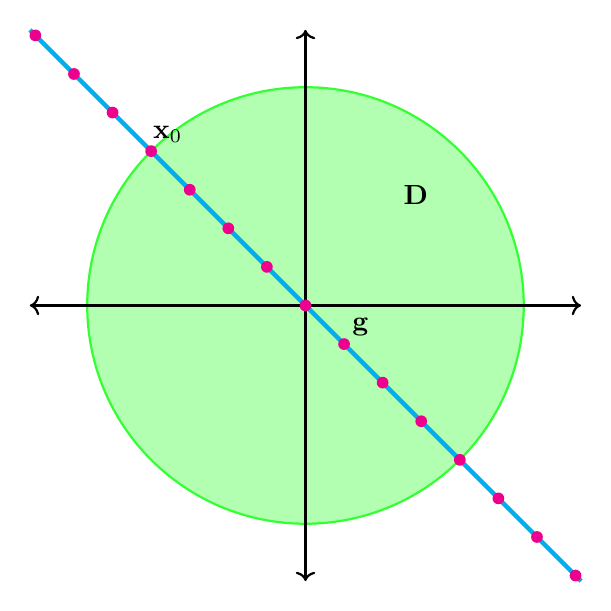
\begin{tikzpicture}[scale=0.7]
\draw[green!80,thick,fill=green!30] (0,0) circle (3.9597);

\draw[color=cyan, ultra thick] (-5,5) -- (5,-5);
\draw[color=black, thick,->] (0,0) -- (5,0);
\draw[color=black, thick,->] (0,0) -- (-5,0);
\draw[color=black, thick,->] (0,0) -- (0,5);
\draw[color=black, thick,->] (0,0) -- (0,-5);
\node at (0,0) [color=magenta,circle,fill,inner sep=1.5pt]{};

\node at (-0.7,0.7) [color=magenta,circle,fill,inner sep=1.5pt]{};
\node at (-1.4,1.4) [color=magenta,circle,fill,inner sep=1.5pt]{};
\node at (-2.1,2.1) [color=magenta,circle,fill,inner sep=1.5pt]{};
\node at (-2.8,2.8) [color=magenta,circle,fill,inner sep=1.5pt]{};
\node at (-3.5,3.5) [color=magenta,circle,fill,inner sep=1.5pt]{};
\node at (-4.2,4.2) [color=magenta,circle,fill,inner sep=1.5pt]{};
\node at (-4.9,4.9) [color=magenta,circle,fill,inner sep=1.5pt]{};
\node at (0.7,-0.7) [color=magenta,circle,fill,inner sep=1.5pt]{};
\node at (1.4,-1.4) [color=magenta,circle,fill,inner sep=1.5pt]{};
\node at (2.1,-2.1) [color=magenta,circle,fill,inner sep=1.5pt]{};
\node at (2.8,-2.8) [color=magenta,circle,fill,inner sep=1.5pt]{};
\node at (3.5,-3.5) [color=magenta,circle,fill,inner sep=1.5pt]{};
\node at (4.2,-4.2) [color=magenta,circle,fill,inner sep=1.5pt]{};
\node at (4.9,-4.9) [color=magenta,circle,fill,inner sep=1.5pt]{};
\node at (-2.5,3.1) [color=black]{$\mathbf{x}_0$};
\node at (1.0,-0.4) [color=black]{$\mathbf{g}$};
\node at (2,2) [color=black]{$\Dd$};
\end{tikzpicture}
\caption*{Figure corresponding to the solution of Problem \ref{prob:grouplemma}.}
\end{figure}


\begin{sol}{prob:grouplemma} We show that if (i) and (iii) both fail, then (ii) must hold. Since (i) fails, we may choose an $\mathbf{x}_0 \in \mathcal{G}$ with $\mathbf{x}_0 \ne \mathbf{0}$. Let $\Dd$ denote the closed disc about $\mathbf{0}$ passing through $\mathbf{x}_0$. The set $(\mathcal{G}\setminus\{\mathbf{0}\}) \cap \Dd$ is nonempty (containing, for example, $\mathbf{x}_0$). Since (iii) fails, this set is also finite. Let $\mathbf{g}$ be any element of $(\mathcal{G}\setminus\{\mathbf{0}\}) \cap \Dd$ minimizing the Euclidean distance to $\mathbf{0}$ (among elements of $(\mathcal{G}\setminus\{\mathbf{0}\}) \cap \Dd$). 

As $\mathbf{g}$ is a nonzero vector belonging to the one-dimensional subspace $V:= \{(x,y): x+y=0\}$ of $\R^2$, we have that $V = \R\mathbf{g}$. We leverage this observation to show that $\mathbf{g}$ generates $\mathcal{G}$. (Hence, (ii) holds!) It is enough to show that an arbitrarily chosen $\mathbf{x} \in \mathcal{G}$ belongs to $\langle \mathbf{g}\rangle$. Since $\mathcal{G} \subset V$, we may write $\mathbf{x} = t\mathbf{g}$, where $t \in \R$. Then $\{t\} \mathbf{g} = \mathbf{x} - \lfloor t\rfloor \mathbf{g} \in \mathcal{G}$. (Here $\{t\} = t -\lfloor t\rfloor$ denotes the fractional part of $t$.) Since $0 \le \{t\} < 1$, the vector $\{t\}\mathbf{g}$ is an element of $\mathcal{G}$ closer to the origin than $\mathbf{g}$. This contradicts the choice of $\textbf{g}$ unless $\mathbf{x} -\lfloor t\rfloor\mathbf{g} =\mathbf{0}$. But then $\mathbf{x} = \lfloor t\rfloor \mathbf{g} \in \langle \mathbf{g}\rangle$. 
\end{sol}


\begin{sol}{prob:almostunittheorem} In view of Problem \ref{prob:grouplemma}, it is enough to show that each closed disc about $\mathbf{0}$ intersects $\Ll(\Uu)$ in a finite set.

Let $\Dd$ be the closed disc of radius $R$ centered at $\mathbf{0}$. Every element of $\Dd \cap \Ll(\Uu)$ can be written as $\Ll(\varepsilon)$ where $1 \le \varepsilon \le e^R$ and $|\varepsilon'| \le e^{R/2}$. As a consequence of Problem \ref{prob:discretelattice}, there are only finitely many possibilities for $\varepsilon$ and hence only finitely many possibilities for $\Ll(\varepsilon)$. 
\end{sol}

\begin{sol}{prob:all1} Since $\theta^3=D$ and $D$ is cubefree, $0 \le 3 v_p(\theta) = v_p(D) < 3$. Hence, $v_p(\theta)=0$ and $|\theta|_p=1$. Also, $|\omega|_p^3 = |\omega^3|_p = |1|_p = 1_p$, so that $|\omega|_p=1$.

Each of $\mu, \mu', \mu'' \in \Z[\theta, \omega]$. Since $\Z\subset \Z_p$ and $\theta, \omega \in \Z_p^{\times}$, we have $\Z[\theta,\omega] \subset \Z_p$. Hence, $|\mu|_p, |\mu'|_p, |\mu''|_p \le 1$. But $|\mu|_p |\mu'|_p |\mu''|_p = |\mu \mu' \mu''|_p = |1|_p=1$. So it must be that $|\mu|_p, |\mu'|_p, |\mu''|_p = 1$.
\end{sol}

\begin{sol}{prob:notconstantzero}\index{$x^3-Dy^3=1$, finiteness of solutions}\index{cubic Pellian equation} Fix $r \in \Z$. For each $m\in \Z$, set $E(m) = \mu^r \nu^m + \omega \mu'^r \nu'^m + \omega^2 \mu''^r \nu''^m$. The equation $E(m)=0$ is an equation involving only elements of $L$ and field operations in $L$. At present, our attention is fixed on the embedded copy of $L$ inside $\Q_p$, but if $E(m)=0$ holds in that copy of $L$, it holds in the OG\footnote{Original Gauss} version of $L$, which is a subfield of $\C$.  

Back in the complex numbers, $|\mu| = \mu > 1$. (Here and below $|\cdot|$ is the usual complex absolute value.) Moreover, $1 = \mu|\mu'\mu''| = \mu |\mu'|^2$, so that $|\mu'| = |\mu''| = 1/\mu < 1$. It follows that $|\nu| = \nu >1$ while $|\nu'| = |\nu''| < 1$. As a consequence, 
\[ |\omega \mu'^r \nu'^m + \omega^2 \mu''^r \nu''^m| \le |\mu'^r|\cdot |\nu'|^m + |\mu''^r| \cdot |\nu''|^m < 1\]
for all large enough positive integers $m$, and
\[ |E(m)| \ge |\mu^r \nu^m| - |\omega \mu'^r \nu'^m + \omega^2 \mu''^r \nu''^m| \ge |\mu^r| \nu^m - 1 > 0 \]
for all sufficiently large $m$.

Therefore, if we pick $m$ as a large enough positive integer, then $E(m)\ne 0$ (and this holds whether we are thinking of $L$ as inside $\C$ or inside $\Q_p$). So from the Strassmann series machinery that we have built up, $E(m)=0$ for only finitely many integers $m$. (Note that this finiteness does \emph{not} follow from the bounds over $\C$ that we derived above. Those bounds imply that $E(m)=0$ for only finitely many positive integers $m$, but they say nothing useful about negative integers $m$.) Finally, letting $r$ range from $0$ to $p-1$, we see that $\mu^n + \omega \mu'^n + \omega^2 \mu''^n=0$ for only finitely many $n\in \Z$.
\end{sol}


\begin{rmk} We can shorten the argument using the Remark following the solution to Problem \ref{ex:KC}. If $E(m)=0$ for all $m \in \Z$, then each term in the list $\nu, \nu', \nu''$ is repeated. But, working again in $\C$,
\[ |\nu| = \nu > 1 > |\nu'| = |\nu''|,\] and so $\nu$ is not repeated.
\end{rmk}

\begin{sol}{prob:strikingcor} Suppose $n^3+1$ has all prime factors from $\mathcal{P}$. Then $n^3+1 = \prod_{p \in \Pp} p^{v_p}$ for some nonnegative integers $v_p$. Writing each $v_p = 3e_p +r_p$, where $r_p \in \{0,1,2\}$, 
\[ n^3+1 = (-D)y^3 \qquad\text{for}\qquad D =\prod_{p\in \Pp} p^{r_p}, \quad y = -\prod_{p\in\Pp}p^{e_p}. \] 
Hence, $(-n,y)$ is an integer solution to $X^3-DY^3=1$. 

By construction, $D\in \mathcal{D}$. If $D=1$, then $n^3$ and $n^3+1$ are positive perfect cubes differing by $1$. But the smallest difference between positive perfect cubes is $2^3-1^3=7$. Thus, $D \in \mathcal{D}\setminus \{1\}$.

By Problem \ref{prob:notconstantzero}, each equation $X^3-DY^3=1$, with $D \in \mathcal{D}\setminus \{1\}$, has finitely many integer solutions. Since $\#\mathcal{D}$ is finite, we conclude that there are finitely many $n$ for which $n^3+1$ has all prime factors from $\Pp$. To deduce that the largest prime factor of $n^3+1$ tends to infinity, choose $\Pp$ as the set of primes up to an arbitrarily prescribed bound.
\end{sol}


\begin{challenge}\index{$x^3-Dy^3=k$, finiteness of solutions} Keep the same assumptions and notation from the proof of the theorem. In this exercise, you will show that for each nonzero integer $k$, the equation $x^3-Dy^3=k$ has finitely many integer solutions $x,y$. Equivalently, there are finitely many pairs of integers $x,y$ with $\Nm(x-y\theta)=k$.
\vspace{-0.12in}
\begin{enumerate}
\item[(a)] Show that the ring $\Z[\theta]/k\Z[\theta]$ is finite, and that in fact $\#\Z[\theta]/k\Z[\theta] = |k|_{\infty}^3$.
\item[(b)] Prove that if $\kappa \in \Z[\theta]$ has $\Nm\kappa=k$, then $\kappa \Z[\theta] \supset k\Z[\theta]$. Deduce from (a) that there are finitely many possibilities for $\kappa$, up to associates. 
\item[(c)] Suppose $\kappa \in \Z[\theta]$ has $\Nm\kappa=k$. Prove that there  are finitely many $u \in \mathcal{U}$ (same meaning as above --- positive units in $\Z[\theta]$) for which $u\kappa$ has the form $x-y\theta$ for some $x,y \in \Z$. Conclude!
\end{enumerate}
\end{challenge}

\begin{challenge}[continuation] Fix a finite set of primes $\mathcal{P}$ and a nonzero integer $d$. Show that there are finitely many $n \in \Z$ such that both $n$ and $n+d$ have all of their prime factors belonging to $\mathcal{P}$.
\end{challenge}


\begin{rmk} As stated on Set \#12, Delaunay and Nagell showed that $x^3-Dy^3=1$ has at most one integer solution with $y\ne 0$. It was discovered by Skolem \cite{skolem} that their theorem can be established by $p$-adic methods. Skolem's proof uses arithmetic in extensions of $\Q_3$; a more elementary $p$-adic proof can be found in lecture notes of Ljunggren \cite{ljunggren}.
\end{rmk}



\let\oldaddcontenttsline\addcontentsline
\renewcommand{\addcontentsline}[3]{}
\begin{thebibliography}{11}
\bibitem{ljunggren} W. Ljunggren,
\emph{Diophantine equations: a $p$-adic approach}. Notes by {R.\,R.} Laxton from a 1968 lecture course at the University of Nottingham.

\bibitem{skolem} T. Skolem,
\emph{Anvendelse av 3-adisk analyse og \textsubscript{''}bikropper`` til bevis for noen satser angående visse kubiske ubestemte ligninger}. Norsk Mat. Tidsskr. \textbf{34} (1952), 45--51.

\end{thebibliography}
\let\addcontentsline\oldaddcontentsline
\chapter*{Solutions to Set \#13}
\addcontentsline{toc}{chapter}{Solutions to Set \#13}
\markboth{Solutions to Set \#13}{Solutions to Set \#13}
\label{set12sols}

\begin{sol}{prob:fundamentalidentity}\index{Teichm\"{u}ller representatives}
%The proof is similar to the argument used in Problem \ref{prob:newbern0}. 
When $p-1\mid k$, every term in the sum is $1$, and $\sum_{u=1}^{p-1} \omega(u)^{k} = p-1 = \one_{p-1\mid k} (p-1)$. 

Now suppose that $p-1\nmid k$.
Recall that every finite subgroup of the multiplicative group of a field is cyclic. Thus, we may choose a generator $\zeta$ for the group $\mu_{p-1} = \{\omega(1), \dots, \omega(p-1)\}$ of $(p-1)$th roots of unity in $\Q_p$. Since $\zeta^{(p-1)k} = 1$ and $\zeta^k \ne 1$,
\begin{align*} \sum_{u=1}^{p-1} \omega(u)^k &= \sum_{j=1}^{p-1} (\zeta^j)^k = \sum_{j=1}^{p-1} (\zeta^k)^j \\&= \zeta^k(1+\zeta^k + \dots + \zeta^{(p-2)k}) = \zeta^{k} \frac{1-\zeta^{(p-1)k}}{1-\zeta^{k}} = 0, \end{align*}
which agrees with $\one_{p-1\mid k} (p-1)$ in this case.
\end{sol}

\begin{sol}{prob:betakintegral} By Faulhaber's formula\index{Bernoulli numbers!Faulhaber's formula}\index{Faulhaber's formula} and Exercise \ref{prob:fundamentalidentity},
\begin{align*} \one_{p-1\mid k} (p-1) &= \sum_{u=1}^{p-1} (u + p\vartheta(u))^{k} \\
&= \sum_{u=1}^{p-1} u^k + \sum_{0< j \le k}\binom{k}{j} p^j \sum_{u=1}^{p-1} u^{k-j} \vartheta(u)^j \\
&= B_k p + \sum_{0< j \le k} \binom{k}{j} B_{k-j} \frac{p^{j+1}}{j+1} + \sum_{0< j \le k}\binom{k}{j} p^j \sum_{u=1}^{p-1} u^{k-j} \vartheta(u)^j.
\end{align*}
Shifting $\one_{p-1\mid k}(p-1)$ to the right-hand side and dividing by $pk$,
\[ \beta_k + \sum_{0< j\le k} \frac{1}{k}\binom{k}{j} B_{k-j} \frac{p^j}{j+1} + \sum_{0< j \le k}\frac{1}{k}\binom{k}{j}p^{j-1} \sum_{u=1}^{p-1} u^{k-j}\vartheta(u)^j=0. \]
This becomes the relation claimed in the problem statement after the substitution $\binom{k}{j} = \frac{k}{j} \binom{k-1}{j-1}$.
\end{sol}

\begin{sol}{prob:adams}\index{Bernoulli numbers!Adams' theorem} Suppose the claim is false and let $k$ be the smallest positive integer with $\beta_k\notin \Z_{p}$. We will derive a contradiction from the relation
\begin{equation}\tag{*} \beta_k + \sum_{0 < j \le k} \binom{k-1}{j-1} B_{k-j}\frac{p^{j}}{j(j+1)}+\sum_{0 < j \le k}\binom{k-1}{j-1}\frac{p^{j-1}}{j}\sum_{u=1}^{p-1}u^{k-j}\vartheta(u)^j =0\end{equation}
established in Problem \ref{prob:betakintegral}.

Let $j$ be an integer in the range $0 < j \le k$. We argue below that the $j$th term in both of the above sums is $p$-adically integral. It is then immediate from (*) that $\beta_{k} \in \Z_{p}$, contrary to our choice of $k$.

We start with the first of the two sums. Observe that
\begin{align*} v_p\left(\frac{p^j}{j(j+1)}\right) &= j - v_p(j(j+1)) \ge j - v_p((j+1)!) \\&> j - \frac{j+1}{p-1} \ge j -\frac{j+1}{2} = \frac{j-1}{2} \ge 0. \end{align*}
Hence, $p^j/j(j+1) \in p\Z_{p}$. Since $\binom{k-1}{j-1} \in \Z$, to complete the proof that $\binom{k-1}{j-1} B_{k-j} p^j/j(j+1) \in \Z_{p}$ it is enough to establish that $pB_{k-j} \in \Z_{p}$. But this follows from our choice of $k$: If $0 < j < k$, then $k-j$ is a positive integer smaller than $k$, so that $\beta_{k-j} \in \Z_{p}$. Hence, $pB_{k-j} - \one_{p-1\mid k-j}(p-1) = p(k-j)\beta_{k-j}  \in p\Z_{p}$, and $pB_{k-j} \in \Z_{p}$. If $j=k$, then $pB_{k-j} = pB_0=p$, which is also in $\Z_{p}$. 

The second sum is easier. There it is clear that the $j$th term lies in $\Z_{p}$ as long as $p^{j-1}/j$ is $p$-adically integral. Integrality is obvious when $j=1$. When $j\ge 2$, we can argue as follows: $v_p\big(\frac{p^{j-1}}{j}\big) = j-1 - v_p(j) \ge j-1 - v_p(j!) > j-1 - \frac{j}{p-1} \ge j-1 -\frac{j}{2}  \ge 0$. (This argument actually shows a bit more: If $j\ge 2$, then $p^{j-1}/j \in p\Z_{p}$.)

\begin{rmk} Note that   $k\beta_{k} = B_k - \frac{\one_{p-1 \mid k} (p-1)}{p} = B_k +\frac{\one_{p-1\mid k}}{p}- \one_{p-1\mid k}$. Thus, $\beta_k\in \Z_{p}$ implies $B_k +\frac{\one_{p-1\mid k}}{p} \in \Z_{p}$, recovering the result of Exercise \ref{prob:newbern2}. 
\end{rmk}
\end{sol}



\begin{sol}{prob:prekummer} Let $p\ge 5$ and let $k\in 2\Z^{+}$. We refine the analysis appearing in the solution to Problem \ref{prob:adams}. Label the two sums in (*) as $\sum_1$ and $\sum_2$.

We will show that the $j$th term of $\sum_1$ lies in $p\Z_{p}$ whenever $0 < j \le k$ and that the $j$th term of $\sum_2$ belongs to $p\Z_{p}$ whenever $1 < j \le k$. Taking (*) modulo $p\Z_{p}$, we deduce that $\beta_k + \sum_{u=1}^{p-1}u^{k-1}\vartheta(u)\in p\Z_{p}$, as required.

For the second sum there is almost nothing to do. We noted at the end of the solution to Problem \ref{prob:adams} that $\frac{p^{j-1}}{j} \in p\Z_{p}$ once $j\ge 2$. (There we only needed $p\ge 3$.) As the other factors in the terms of $\sum_2$ are $p$-adic integers, our claim for $\sum_2$ follows.

Since $k$ is even, the only odd integer $j$ which contributes to $\sum_1$ is $j=k-1$. For this $j$, we have $\binom{k-1}{j-1} B_{k-j} \frac{p^j}{j(j+1)} = (k-1)B_1 \frac{p^{k-1}}{k(k-1)} = -\frac{1}{2}\frac{p^{k-1}}{k}$. We already observed that $\frac{p^{k-1}}{k} \in p\Z_{p}$, while clearly $-\frac{1}{2} \in \Z_p$ ($p$ is odd). Hence, the term of $\sum_1$ corresponding to $j=k-1$ belongs to $p\Z_{p}$. Suppose now that $j$ is even and $0 < j \le k$. If $0 < j < k$, the $p$-integrality of $\beta_{k-j}$ established in Problem \ref{prob:adams} implies that
\[ pB_{k-j} = p(k-j)\beta_{k-j} + \one_{p-1\mid k-j}(p-1) \in \Z_{p}. \]
If $j=k$, then $pB_{k-j} = pB_{0} = p$, and this also belongs to $\Z_p$. Thus, it will suffice to show that $\frac{p^{j-1}}{j(j+1)} \in p\Z_{p}$. This follows upon observing that
\begin{align*}
v_p\left(\frac{p^{j-1}}{j(j+1)}\right)  &= j-1 - v_p(j(j+1)) \ge j-1 - v_p((j+1)!) \\
&> j-1 - \frac{j+1}{p-1} \ge j-1-\frac{j+1}{4} > 0,
\end{align*}
keeping in mind for the last step that $j\ge 2$.
\end{sol}

\begin{sol}{prob:kummer}\index{Bernoulli numbers!Kummer's congruence}  We are assuming that $p-1$ does not divide the even integer $k$, so that $p\ge 5$. Since $k$ and $k'$ are congruent mod $p-1$, the integer $k'$ is also not divisible by $p-1$. By Problem \ref{prob:prekummer}, 
\begin{align*} \frac{B_k}{k} &= \beta_k \equiv -\sum_{u=1}^{p-1} u^{k-1}\vartheta(u) \pmod{p\Z_{p}}, \\ \frac{B_{k'}}{k'} &= \beta_{k'} \equiv -\sum_{u=1}^{p-1} u^{k'-1}\vartheta(u) \pmod{p\Z_{p}}. \end{align*}
Suppose without loss of generality that $k'\ge k$ and write $k' = k + (p-1)q$. Then $u^{k'-1} = u^{k-1} u^{(p-1)q} \equiv u^{k-1}\pmod{p\Z_p}$, by Fermat's little theorem. (To apply Fermat, we identify $\Z_p/p\Z_p$ with $\Z/p$, invoking Problem \ref{prob:58}.) Substituting above, $\frac{B_k}{k} \equiv \frac{B_{k'}}{k'}\pmod{p\Z_{p}}$.\end{sol}

\begin{rmk} Call an odd prime $p$ \textsf{regular}\index{regular prime} if $p$ does not divide the numerator of any of $B_2, B_4, \dots, B_{p-3}$. In the middle of the 19th century, Kummer showed that Fermat's last theorem\index{Fermat's last theorem} for the exponent $p$ holds for all regular primes $p$. That is, if $p$ is a regular prime, then $x^p+y^p=z^p$ has no solutions in integers $x,y,z$ with $xyz\ne 0$ (see the books of Ribenboim \cite{ribenboim} and Washington \cite{washington} for accounts of this work).

All primes smaller than $37$ are regular, while $37$ is not: $B_{32} = -37 \cdot \frac{683 \cdot 305065927}{2\cdot 3\cdot 5 \cdot 17}$. Via Kummer's congruence (the result of Problem \ref{prob:kummer}), it is possible to show that there are infinitely many \underline{ir}regular primes\index{irregular prime} (odd primes that are not regular). We sketch an argument for this due to Carlitz \cite{carlitz}, which nicely illustrates how the facts we have built up about Bernoulli numbers can be put to use. 

Looking at the Remark following the solution to Problem \ref{prob:alternatingsigns}, we see that $|B_{2m}|_{\infty}$ tends to infinity faster than any power of $m$. In particular, as we will use momentarily, $|\frac{B_{2m}}{2m}|_{\infty} > 1$ for all large values of $m$.

Let $p_1,\dots,p_r$ be any finite list of irregular primes, and let $$N = 2\mathop{\mathrm{lcm}}[p_1-1,\dots,p_r-1].$$ We let $k$ run over the positive multiples of $N$ and consider the ratios $B_{k}/k$. From the last paragraph, we can choose $k$ with $|B_k/k|_{\infty} > 1$. Then there is a prime $p$ dividing the numerator of $B_k/k$. Since $p_i-1$ divides $k$ for each $i=1,2,\dots, r$, each of our primes $p_i$ appears in the denominator of $B_k$, and so also in the denominator of $B_k/k$ (by the Clausen--von Staudt theorem, Exercise \ref{ex:vsclast}). Thus, $p$ is not any of $p_1,\dots,p_r$. A similar argument shows that $p-1$ does not divide $k$ (note that this implies $p\ne 2$). If we let $k'$ denote the reduction of $k$ modulo $p-1$, then $k' \in \{2, 4, 6, \dots, p-3\}$, and by Kummer's congruence, 
\[ \frac{B_{k'}}{k'} \equiv \frac{B_k}{k} \equiv 0 \pmod{p\Z_p}. \] 
Therefore, $p$ divides the numerator of $B_{k'}$, implying that $p$ is an irregular prime not on our initial list. At this point in the proof Euclid is smiling down from heaven.

From the perspective of progress towards Fermat's Last Theorem, it would certainly be more encouraging to know that there are infinitely many \emph{regular} primes. Unfortunately, this question remains wide open! Of course, the urgency of the problem has diminished somewhat in the wake of the full proof of Fermat's Last Theorem by Wiles and Taylor--Wiles.\footnote{The story of which is gloriously recounted in  Joshua Rosenblum and Joanne Sydney Lessner's 2000 musical \emph{Fermat's Last Tango}.}
\end{rmk}

\begin{sol}{prob:glaisherharmonic}\index{harmonic number}\index{Bernoulli numbers!associated congruence for $H_{p-1}$}Let $p\ge 5$ be prime, and let $k = \varphi(p^3)-1$.

The group $(\Z_p/p^3\Z_p)^\times$ can be identified with $(\Z/p^3)^{\times}$, which has order $\varphi(p^3)$. Hence, each $x \in \Z_p^{\times}$ satisfies $x^{\varphi(p^3)} \equiv 1\pmod{p^3\Z_p}$, and $x^{k} \equiv \frac1x \pmod{p^3 \Z_{p}}$. Therefore, working in $\Z_p$ modulo $p^3\Z_{p}$,
\[ H_{p-1} = \sum_{n=1}^{p-1} \frac{1}{n} \equiv \sum_{n=1}^{p-1} n^{k} = k\frac{p^2}{2} B_{k-1} + \sum_{2 \le j \le k}\binom{k}{j} B_{k-j} \frac{p^{j+1}}{j+1}.
\]
In this last expression, the term $pB_k$ has been dropped from Faulhaber's formula, which is harmless as $k$ is odd and larger than $1$.

Continuing, we argue that every term of the sum on $j$ belongs to $p^3 \Z_p$. Suppose $j \ge 3$. Since $pB_{k-j} \in \Z_{p}$ (as follows from Problem \ref{prob:newbern2} or \ref{prob:adams}), 
\begin{align*} v_p\left(\binom{k}{j} B_{k-j} \frac{p^{j+1}}{j+1}\right) &= v_p\left(\binom{k}{j} pB_{k-j} \frac{p^{j}}{j+1}\right) \ge j - v_p(j+1) \\ &\ge j - v_p((j+1)!) > j - \frac{j+1}{p-1} \ge j - \frac{j+1}{4} \ge 2.
\end{align*}
This shows that each term with $j\ge 3$ belongs to $p^3 \Z_{p}$. The remaining term, corresponding to $j=2$, is $\binom{k}{2} B_{k-2} \frac{p^3}{3}$. As $k-2\equiv p-4\not\equiv 0\pmod{p-1}$, we have that $B_{k-2} \in \Z_{p}$. Hence, $\binom{k}{2} B_{k-2} \frac{p^3}{3} \in p^3 \Z_p$.

Collecting our results so far, $H_{p-1} \equiv k \frac{p^2}{2} B_{k-1} \pmod{p^3\Z_p}$. Kummer, as incarnated in Problem \ref{prob:kummer}, now steps in to tell us that $$\frac{B_{k-1}}{k-1} \equiv \frac{B_{p-3}}{p-3}\pmod{p\Z_p}.$$
Therefore, 
\[ B_{k-1} \equiv (k-1) \frac{B_{p-3}}{p-3} \equiv \frac{2}{3} B_{p-3}\pmod{p\Z_p}, \] and \[ H_{p-1} \equiv k \frac{p^2}{2} B_{k-1} \equiv k\frac{p^2}{3} B_{p-3}\equiv -\frac{p^2}{3} B_{p-3}\pmod{p^3\Z_{p}}.\] 

From this last congruence for $H_{p-1}$, we have $H_{p-1} \in p^3 \Z_p \Longleftrightarrow B_{p-3} \in p \Z_p$. This equivalence is the concluding assertion of the problem statement.
\end{sol}

\begin{rmk} This problem brings to a close our study of the Bernoulli numbers. For everything you ever wanted to know about this subject but were afraid to ask, see Chapter 15 in the book of Ireland and Rosen \cite{IR}, Chapter 9 in Cohen's volume \cite{cohenbook}, and the recent book \cite{bernoulli} by T. Arakawa, T. Ibukiyama, and M. Kaneko. A bibliography with $\approx$ 3000 books and papers related to Bernoulli numbers has been compiled by Karl Dilcher, Ladislav Skula, and Ilja Sh. Slavutskii \cite{bernoullibib}. 
\end{rmk}


\begin{sol}{prob:strassdivide} Since $F(r)=0$, we have  $F(x) = F(x) - F(r) = \sum_{k\ge 0} a_k (x^k -r^k) =\sum_{k\ge 0} a_k (x-r) \sum_{j=0}^{k-1}x^j r^{k-1-j}$. 

Let $u_{k,j} = \one_{0\le j < k} \cdot a_k x^{j} r^{k-1-j}$. If we put $\epsilon_N:= \max_{n\ge N} |a_n|_p$, then 
\[ |u_{k,j}|_p \le \one_{0 \le j < k} |a_k|_p \le \epsilon_N\qquad\text{whenever $j\ge N$ or $k\ge N$}. \] Moreover, $\epsilon_N\to 0$ (as $F$ is a Strassmann series). So by Exercises \ref{prob:91} and \ref{prob:92}, $\sum_{k}\sum_{j} u_{k,j}$ and $\sum_{j}\sum_{k} u_{k,j}$ both converge, and to the same value. Hence,
\begin{align*} F(x)  = (x-r) \sum_{k} \sum_{j} u_{k,j} &=(x-r) \sum_{j} \sum_{k} u_{k,j}\\
&= (x-r) \sum_{j\ge 0}x^j\sum_{k > j}a_k r^{k-1-j}.
\end{align*}
Here the final sum on $k$ is exactly what we called $b_j$. Therefore, if we set $G(T) = \sum_{j\ge 0} b_j T^j$, we have shown that $G(x)$ converges for all $x\in\Z_p$ (i.e., $G(T)$ is Strassmann) and that $F(x) = (x-r) G(x)$ for all such $x$.

Now we suppose that the Strassmann degree $K$ of $F(T)$ is at least $1$ and prove that the Strassmann degree of $G(T)$ is $K-1$. If $j < K-1$, then
\[ |b_j|_p \le \max_{k > j} |a_k r^{k-1-j}|_p \le \max_{k} |a_k|_p = |a_K|_p. \]
When $j=K-1$,
\[ |b_{K-1}|_p = \left|a_K + \sum_{k>K} a_k r^{k-K}\right|_p.\]
This last sum on $k$ satisfies $$\bigg|\sum_{k > K} a_k r^{k-K}\bigg|_p \le \max_{k > K} |a_k r^{k-K}|_p \le \max_{k > K} |a_k|_{p} < |a_K|_p.$$ So by survival of the greatest, $|b_{K-1}|_p = |a_K|_p$. Finally, when $j \ge K$,
\[ |b_j|_p \le \max_{k>K} |a_k r^{k-1-j}|_p \le \max_{k > K} |a_k|_p < |a_K|_p. \]
Hence, the maximum value of $|b_j|_p$ is $|a_K|_{p}$, and this maximum is attained for the last time at $j=K-1$. Therefore, $G(T)$ has  Strassmann degree $K-1$.
\end{sol}

\begin{challenge} Recall our notation $\Q_p\langle T\rangle$ for the ring of Strassmann series.  Problem \ref{prob:strassdivide} establishes a version of the Root-Factor theorem for Strassmann series viewed as functions on $\Z_p$. Show that the Root-Factor theorem is also valid at the level of formal power series. More precisely,  show that if $r \in \Z_p$ is a root of $F(T) \in \Q_p\langle T\rangle$, then $F(T) = (T-r) G(T)$, where $G(T) \in \Q_p\langle T\rangle$ is the power series constructed in the preceding solution. 
\end{challenge}

\begin{challenge}\mbox{ }
\begin{enumerate}
\vspace{-0.12in}
\item[(a)] Prove that if $F(T), G(T)$ are nonzero elements of $\Q_p\langle T\rangle$, then the Strassmann degree of $FG$ is the sum of the Strassmann degrees of $F$ and $G$.
\item[(b)] Show that if $X(T)$ is a Strassmann series with all coefficients from $\Z_p$, then $1+pT \cdot X(T)$ is a unit in $\Q_p\langle T\rangle$, with inverse $1 - pT\cdot X(T) + p^2 T^2 \cdot X(T)^2 - p^3 T^3 \cdot X(T)^3 + \dots$, for an appropriate interpretation of the infinite series.
\item[(c)] Establish that the units in $\Q_p\langle T\rangle$ are precisely the elements of Strassmann degree $0$.
\end{enumerate}
\end{challenge}




\begin{sol}{ex:strassthm}\index{Strassmann series!number of zeros bounded by Strassmann degree}\index{Strassmann's theorem} Suppose to start off that  $F(T) = \sum_{k\ge 0} a_k T^k$ has Strassmann degree $K=0$. Then $|a_{0}|_p > |a_k|_p$ for every $k\ge 1$. Hence, for every $x\in \Z_p$, we have $|\sum_{k\ge 1} a_k x^k|_p \le \max_{k\ge 1}|a_k|_p < |a_0|_p$  and
\[ |F(x)|_p = \bigg|a_0 + \sum_{k\ge 1} a_k x^k\bigg|_p \ge |a_0|_p - \bigg|\sum_{k\ge 1} a_k x^k\bigg|_p > 0.\]
Therefore, $F$ has no zeros in $\Z_p$ (and no zeros is ``at most $K=0$ zeros''), 

Assuming the general claim fails,  choose a counterexample $F(T)$ whose Strassmann degree $K$ is as small as possible. Then $K\ge 1$. By assumption, $F$ has more than $K$ distinct zeros in $\Z_p$; pick one of these and call it $r$. By Exercise \ref{prob:strassdivide}, we can find a Strassmann series $G(T)$ of Strassmann degree $K-1$ with $F(x) = (x-r) G(x)$ for all $x \in \Z_p$. As $K-1 < K$, we know that $G$ has at most $K-1$ distinct zeros in $\Z_p$. But each zero of $F$, other than (possibly) $r$, is a zero of $G$. Thus, there are at most $1+(K-1)= K$ zeros of $F$ in $\Z_p$, contradicting the choice of $F(T)$.
\end{sol}

% \begin{rmk} Let $\overline{\Q}_p$ denote the algebraic closure of $\Q_p$. The $p$-adic absolute value has a unique extension from $\Q_p$ to $\overline{\Q}_p$ (\cite[Chapter 7]{cassels86}, \cite[Chapter 6]{gouvea}, or \cite[Chapter 2, \S3]{robert}) and each Strassmann series $F(T) \in \Q_p[[T]]$ has precisely $K$ zeros counted ``with multiplicity'' in the corresponding closed unit disc $\Oo$ of $\overline{\Q}_p$. Here, as before, $K$ denotes the Strassmann degree of $F$. 
\begin{rmk}
It is enlightening to view Strassmann's theorem through the lens of the \textsf{Weierstrass preparation theorem for $\Q_p$}: \emph{Every Strassmann series $F(T)$ with Strassmann degree $K$ admits a factorization $F(T) = U(T) V(T)$ where $U(T) \in \Q_p[T]$ is polynomial whose degree and Strassmann degree are both $K$ and $V(T) = 1 + p \tilde{V}(T)$ for a Strassmann series $\tilde{V}(T) \in \Z_p[[T]]$.} You might try to prove this theorem yourself by imitating our second solution to Problem \ref{prob:uniquezero}. If you get stuck, look at \cite[pp.~54--55]{lewis} or \cite[pp.~166--167]{skolem}.\index{Weierstrass preparation theorem for $\Q_p$}

Suppose we have factored $F(T)=U(T) V(T)$ as in the Weierstrass preparation theorem. Then $V(x)\in 1+p\Z_p$ for all $x \in \Z_p$; in particular, $V(x)\ne 0$.  Since $F(x) = U(x) V(x)$ for all $x \in \Z_p$, we deduce that $F$ and $U$ have the same zeros in $\Z_p$. But $U$, as a polynomial of degree $K$, has at most $K$ zeros in $\Q_p$, and a fortiori at most $K$ zeros in $\Z_p$.\footnote{Actually, each of its $\Q_p$-zeros is a $\Z_p$-zero. Since $U$ has the same degree as Strassmann degree, scaling by an appropriate power of $p$ turns $U$ into a polynomial with $\Z_p$-coefficients and leading coefficient a $p$-adic unit. Each $\Q_p$-root of such a polynomial belongs to $\Z_p$. Cf.~the proof of the Lemma in the solution to Problem \ref{prob:mahlerSML}.} Thus, the Weierstrass preparation theorem can be viewed as ``explaining'' Strassmann's theorem. This reasoning is very close to Strassmann's original proof; the Weierstrass preparation theorem as stated here follows from the assertions ``1'', ``1$'$'', and ``3'' appearing on page 21 of \cite{strassmann}. 
\end{rmk}



\begin{sol}{prob:constantcheck} Referring back to Set \#11, for each $A \in p\Z_{p}$ the constant term $C_{A,0}$ of $\Binom(1+A,T)$ is 
\[ C_{A,0} = \sum_{k\ge 0} s(k,0) \frac{A^k}{k!} = s(0,0) \frac{A^0}{0!} = 1. \]
Therefore, the constant term of $$F_{r,\pm}(T) = \alpha^{r}\,\Binom(1+a;T) - \beta^{r}\,\Binom(1+b;T) \mp (\alpha-\beta)$$ is $\alpha^r-\beta^r \mp (\alpha-\beta)$. This vanishes precisely when $\frac{\alpha^r-\beta^r}{\alpha-\beta}=\pm 1$. Inspecting the table on Set \#3, we see that when $0\le r \le 9$, we have $\frac{\alpha^r-\beta^r}{\alpha-\beta}=\pm 1$ if and only if $(r,\pm) \in \{(1,+), (2,+), (3,-), (5,-)\}$. 

For all other values of $(r,\pm)$ one computes directly (see the tables at the top of this page) that $F_{r,\pm}(0)$ is an $11$-adic unit.

\setlength{\tabcolsep}{7pt}
\begin{table}[t]
    \centering
    \begin{tabular}{r || c  c  c  c  c c c c c c}
      $r$ &  0 & 1 & 2 & 3 & 4 & 5 & 6 & 7 & 8 & 9 \\\midrule
      $F_{r,+}(0)\bmod{11\Z_{11}}$    & 9 & 0 & 0 & 7 & 3 & 7 & 8 & 1 & 3 & 8 \\
    \end{tabular}
\vskip 0.1in
    \begin{tabular}{r || c  c c  c  c c c c c c}
      $r$ &  0 & 1 & 2 & 3 & 4 & 5 & 6 & 7 & 8 & 9 \\\midrule
      $F_{r,-}(0)\bmod{11\Z_{11}}$  
      & 2 &4  & 4& 0 & 7 & 0 & 1 & 5 & 7 & 1 \\
    \end{tabular}
    \caption*{Constant terms of $F_{r,\pm}(T)$ modulo $11\Z_{11}$.}
\end{table}
    
Now let $j\ge 1$. The $T^j$-coefficient of $F_{r,\pm}(T)$ is given by 
\[ \alpha^r C_{a,j}-\beta^r C_{b,j}= \sum_{k \ge j} s(k,j) \left(\alpha^r \frac{a^k}{k!} - \beta^r \frac{b^k}{k!}\right).  \]
For each $k\ge j$, we have $v_{11}(a^k/k!), v_{11}(b^k/k!) \ge k - v_{11}(k!) >  k - \frac{k}{10} = 0.9k \ge 0.9j$. Therefore,
\[ |\alpha^r C_{a,j}-\beta^r C  _{b,j}|_{11} \le \max_{k\ge j} \left|s(k,j) \left(\alpha^r \frac{a^k}{k!} - \beta^r \frac{b^k}{k!}\right)\right|_{11} \le 11^{-0.9j}. \]
In particular, every nonconstant coefficient of $F_{r,\pm}(T)$ has $11$-adic absolute value less than $1$.

We conclude that, apart from the four specified values of $(r,\pm)$, the series $F_{r,\pm}(T)$ has constant term an $11$-adic unit and all other terms belonging to $11\Z_{11}$. Hence, $F_{r,\pm}(T)$ has Strassmann degree $0$ and no zeros in $\Z_p$ (by Exercise \ref{ex:strassthm}).
\end{sol}

\begin{sol}{prob:easycases} The $T$-coefficient of $F_{r,\pm}(T)$ is \[\alpha^r C_{a,1} - \beta^{r} C_{b,1} = \sum_{k\ge 1} s(k,1) \left(\alpha^r \frac{a^k}{k!} - \beta^r\frac{b^k}{k!}\right). \]
Reasoning as in the solution to Problem \ref{prob:constantcheck},  the terms of the right-hand sum with $k\ge 2$ make a contribution bounded in $11$-adic absolute value by $11^{-0.9\cdot 2}$, and hence also bounded by $11^{-2}$ (since no absolute value is strictly between $11^{-1}$ and $11^{-2}$). Keeping in mind that $s(1,1)=1$, we conclude that
\begin{equation}\tag{*} \alpha^r C_{a,1} - \beta^{r} C_{b,1} \equiv \alpha^r a - \beta^r b \pmod{11^2\Z_{11}}. \end{equation}
Plugging our approximations of $\alpha$ and $a$ into (*), we find that the $T$-coefficient
\begin{align*} \text{of $F_{1,+}$ is }&\equiv 4\cdot 11\pmod{11^2\Z_{11}}, \\
\text{of $F_{2,+}$ is }&\equiv 8\cdot 11\pmod{11^2\Z_{11}},\\
\text{of $F_{3,-}$ is }&\equiv 0 \pmod{11^2\Z_{11}}, \text{ \emph{and}}\\
\text{of $F_{5,-}$ is }&\equiv 6\cdot 11\pmod{11^2\Z_{11}}.
\end{align*}
So the $T$-coefficients are divisible by $11$ but not $11^2$ for $(r,\pm) = (1,+)$, $(2,+)$, and $(5,-)$.

Let's take stock of what we've shown in this exercise and the last. If $(r,\pm)$ is any of $(1,+), (2,+), (5,-)$, then the constant term of $F_{r,\pm}(T)$ is $0$. The $T$-coefficient has $11$-adic absolute value $11^{-1}$. And the $T^j$ coefficient has $11$-adic absolute value at most $11^{-0.9\cdot 2} < 11^{-1}$, for each $j\ge 2$. It follows that $F_{r,\pm}(T)$ has Strassmann degree $1$. 
% \setlength{\tabcolsep}{7pt}
% \begin{table}
%     \centering
%     \begin{tabular}{r || c | c| c | c}
%       $(r,\pm)$ &  (1,+) & (2,+) & (3,-) & (5,-) \\\hline 
%       $F_{r,+}(0)\bmod{11^2 \Z_{11}}$    & 1\\
%     \end{tabular}
% \end{table}
\end{sol}

\begin{sol}{prob:annoyingcase} We saw already in the solution to Problem \ref{prob:easycases} that $F_{3,-}(T)$ has $T$-coefficient divisible by $11^2$. 

The $T^2$-coefficient of $F_{3,-}(T)$  is given by
\[ \alpha^3 C_{a,2} - \beta^3 C_{b,2} = \sum_{k\ge 2} s(k,2) \left(\alpha^3 \frac{a^k}{k!} - \beta^3 \frac{b^k}{k!}\right). \]
Here the terms of the right-hand sum corresponding to $k\ge 3$ make a contribution bounded in $11$-adic absolute value by $11^{-0.9\cdot 3}$, and hence also by $11^{-3}$. Since $s(2,2)=1$ ($s(2,2)$ is the coefficient of $T^2$ in $T(T-1)$), 
\[ \alpha^3 C_{a,2} - \beta^3 C_{b,2} \equiv \alpha^3 \frac{a^2}{2} - \beta^3 \frac{b^2}{2} \pmod{11^3 \Z_{11}}. \]
Working with the right-hand side, we find that
\[ \alpha^3 C_{a,2} - \beta^3 C_{b,2} \equiv 8\cdot 11^2\pmod{11^3\Z_{11}}.\]
Hence, the $T^2$-coefficient of $F_{3,-}(T)$ is divisible by $11^2$ but not $11^3$.

For every $j\ge 3$, the $T^j$ coefficient of $F_{3,-}(T)$ is bounded in absolute value by $11^{-0.9\cdot 3} < 11^{-2}$. 

Summing up: $F_{3,-}(T)$ has vanishing constant term, $T$-coefficient bounded in absolute value by $11^{-2}$, $T^2$-coefficient with absolute value equal to $11^{-2}$, and $T^j$ coefficients with absolute value strictly smaller than $11^{-2}$ for $j\ge 3$. Therefore, $F_{3,-}(T)$ has Strassmann degree $2$.
\end{sol}

\begin{sol}{ex:finalram}\index{Ramanujan--Nagell equation} If $\frac{\alpha^n-\beta^n}{\alpha-\beta}=\pm 1$, then $F_{r,\pm}(n)=0$, where $r$ is the remainder when $n$ is divided by $10$. In Exercise \ref{prob:constantcheck}, we found that $F_{r,\pm}$ has no zeros in $\Z_p$ (let alone in $\Z$!) except possibly if $(r,\pm) \in \{(1,+), (2,+), (3,-), (5,-)\}$.

In Exercise \ref{prob:easycases}, we showed that $F_{r,\pm}(T)$ has Strassmann degree $1$ for each of $(r,\pm)= (1,+)$, $(2,+)$, and $(5,-)$. By Strassmann's Theorem (Exercise \ref{ex:strassthm}), each corresponding series $F_{r,\pm}(T)$ has at most one zero in $\Z_p$. Similarly, the result of Exercise \ref{prob:annoyingcase} shows that $F_{3,-}(T)$ has at most $2$ zeros in $\Z_p$.

Consequently, there are at most $1+1+1+2 = 5$ integers $n$ for which $\frac{\alpha^n-\beta^n}{\alpha-\beta}=\pm 1$. We know five such integers already: $n=1, 2, 3, 5, 13$. (See the table on Set \#3.) Thus, there can be no others.
\end{sol}

\begin{challenge}[Skolem, Chowla, and Lewis \cite{SCL}] Prove that each integer appears at most three times in the sequence $\{\frac{\alpha^n-\beta^n}{\alpha-\beta}\}_{n\ge 0}$ (for the same $\alpha,\beta$ as above).
\end{challenge}

\begin{challenge}[Cohen and Ljunggren \cite{cohen}] Find all integer solutions to $x^2+11=3^m$.
\end{challenge}

\begin{challenge} What are all of the positive integer solutions to $2x^2+1 = 3^m$? Equivalently: Which squares have ternary expansions consisting entirely of the digit $1$?
\end{challenge}


\let\oldaddcontenttsline\addcontentsline
\renewcommand{\addcontentsline}[3]{}
\begin{thebibliography}{11}
\bibitem{bernoulli} T. Arakawa, T. Ibukiyama, and M. Kaneko, 
\emph{Bernoulli numbers and zeta functions}, Springer Monogr. Math., Springer, Tokyo, 2014.


\bibitem{carlitz} L. Carlitz, \emph{
Note on irregular primes}. Proc. Amer. Math. Soc. \textbf{5} (1954), 329--331.


\bibitem{cohen}
E.\,L. Cohen, \emph{Sur l'équation diophantienne $x^2+11=3^k$}. C. R. Acad. Sci. Paris Sér. A-B 275 (1972), A5--A7.

\bibitem{cohenbook}
H.~Cohen, \emph{Number theory. Vol. II. Analytic and modern tools}, Graduate Texts in Mathematics, vol.~240, Springer, New York, 2007. 

\bibitem{bernoullibib} K.~Dilcher, L.~Skula, and I.~Sh. Slavutskii, \emph{A bibliography of Bernoulli numbers}. Online resource. URL: \url{https://www.mscs.dal.ca/~dilcher/bernoulli.html}

\bibitem{IR} K. Ireland and M. Rosen, \emph{A classical introduction to modern number theory}, second ed., Graduate Texts in Mathematics, vol. 84, Springer-Verlag, New York, 1990.

\bibitem{lewis}{D.\,J.} Lewis, \emph{
Diophantine equations: $p$-adic methods.} In: Studies in Number Theory, MAA Stud. Math., vol. 6, pp. 25--75. Math. Assoc. America, Buffalo, NY, 1969.

\bibitem{ribenboim} P. Ribenboim, \emph{13 lectures on Fermat's last theorem}, Springer-Verlag, New York-Heidelberg, 1979. 

\bibitem{skolem} T.~Skolem, \emph{Ein Verfahren zur Behandlung gewisser exponentialer Gleichungen und diophantischer Gleichungen}. 
%C. r. 8 congr. scand. \`a Stockholm (1934)
Comptes Rendus Congr. Math. Scand. (Stockholm, 1934), 163--188. 

\bibitem{SCL} T.~Skolem, S.~Chowla, and {D.\,J.} Lewis, \emph{The diophantine equation $2^{n+2}-7=x^2$ and related problems}.
Proc. Amer. Math. Soc. \textbf{10} (1959), 663--669.

\bibitem{strassmann} R.~Strassmann, \emph{\"{U}ber den Wertevorrat von Potenzreihen im Gebiet der $\mathfrak{p}$-adischen Zahlen}. J. Reine Angew. Math. \textbf{159} (1928), 13--28.

\bibitem{washington} L.\,C. Washington, \emph{Introduction to cyclotomic fields}, second ed., Graduate Texts in Mathematics, vol. 83, Springer-Verlag, New York, 1997.

\end{thebibliography}
\let\addcontentsline\oldaddcontentsline


%\include{setextras} 


% 
\chapter*{Solutions to Set \#1}
\addcontentsline{toc}{chapter}{Solutions to Set \#1}
\markboth{Solutions to Set \#1}{Solutions to Set \#1}
\label{set0sols}

\begin{sol}{prob:01} 
    \begin{enumerate}
        \item[(a)] First off, $|1|^2 = |1\cdot 1|=|1|$ and $|1| > 0$ (from (i)). Thus, $|1| = 1$. Next, $|-1|^2 = |(-1) (-1)| = |1| = 1$. As $|-1| > 0$, we conclude that $|-1|=1$.
\item[(b)] The proof is the same for the ``standard'' absolute value: By the triangle inequality, $|x| = |(x-y)+y| \le |x-y| + |y|$. Now rearrange.
\item[(c)] Since $|y^{-1}|\cdot |y|= |y^{-1}\cdot y| = |1| = 1$, we have $|y^{-1}| = |y|^{-1}$. So $|xy^{-1}| = |x||y^{-1}| = |x||y|^{-1}$, as claimed.
    \end{enumerate}
\end{sol}

\begin{sol}{prob:02}  Property (i) in the absolute value definition is clear. Property (ii) is also easy: When $x+y=0$, the inequality is obvious. Otherwise, either $x$ or $y$ is nonzero, so that $|x|$ or $|y|$ is $1$. Hence, $1= |x+y| \le |x| + |y|$. To prove (iii), take cases: If $x$ and $y$ are nonzero, both sides are $1$, otherwise both sides are $0$. In this last step we use that fields are integral domains.
\end{sol}

\begin{sol}{prob:03} Property (i) is again clear. Of the remaining two properties, (iii) is quicker to dispense with: If $x$ or $y$ is zero, both sides of (iii) vanish. Otherwise, write $x= p^{v_p(x)} \frac{a}{b}$ and $y=p^{v_p(y)} \frac{c}{d}$, where $p$ does not divide any of $a,b,c,d$. Then $xy = p^{v_p(x)+v_p(y)} \frac{ac}{bd}$, and $p$ does not divide either of $ac$ or $bd$. Hence, $v_p(xy) = v_p(x) + v_p(y)$ and $|xy|_p = p^{-v_p(x)} p^{-v_p(y)} = |x|_p |y|_p$.

To prove (ii) we have to work a bit harder. If $x$, $y$, or $x+y$ is zero, (ii) is trivial. Otherwise, write $x= p^{v_p(x)} \frac{a}{b}$ and $y=p^{v_p(y)} \frac{c}{d}$ as above. The symmetry of (ii) in $x$ and $y$ allows us to assume $v_p(x) \le v_p(y)$. Then $x+y= p^{v_p(x)} \left(\frac{a}{b} + p^{v_p(y)-v_p(x)} \frac{c}{d}\right)$. Since $p^{v_p(y)-v_p(x)}\in \Z$, we can express $p^{v_p(y)-v_p(x)}\frac{c}{d}$ as a fraction with denominator $d$. Hence, $\frac{a}{b} + p^{v_p(y)-v_p(x)} \frac{c}{d} = \frac{N}{bd}$ for some nonzero $N\in \Z$. Write $N = p^{w} N'$, where $w$ is a nonnegative integer and $N'\in \Z$ is not divisible by $p$. Then $x+y = p^{v_p(x)+w} \frac{N'}{bd}$, where neither $N'$ nor $bd$ is divisible by $p$. Hence, $v_p(x+y) = v_p(x) + w \ge v_p(x)$, and $|x+y|_{p} = p^{-v_p(x)} p^{-w} = |x|_p p^{-w} \le |x|_p \le |x|_p + |y|_p$.
\end{sol}


\begin{sol}{prob:05} This is implicit in our solution to Problem \ref{prob:03}.
\end{sol}

\begin{sol}{prob:04} We may assume without loss of generality that $|x| > |y|$. A direct application of the strong triangle inequality gives $|x+y| \le \max\{|x|,|y|\} = |x|$. The strong triangle inequality also implies that $|x| = |(x+y) + (-y)| \le \max\{|x+y|,|-y|\} = \max\{|x+y|,|y|\}$. (We use in this last step that $|-y| = |y|$, which follows from $|-1|=1$.) Since $|x| > |y|$, the maximum here cannot be $|y|$. So it must be $|x+y|$, yielding $|x| \le |x+y|$. Hence, $|x+y| = |x|$.  
\end{sol}


\begin{sol}{prob:06} Since $|2| \le 1$, we see that $|2^{e_1} + \dots + 2^{e_n}| \le  |2|^{e_1} + \dots + |2|^{e_n} \le 1  +\dots + 1 = n$.
To conclude, notice that (a) every positive integer less than $2^n$ is a sum of at most $n$ powers of $2$ (e.g., use the binary representation), while (b) $\sum_{0 \le k \le n} \binom{n}{k}=2^n$, so that $\binom{n}{k} < 2^n$ for every $k$.
\end{sol}

\begin{sol}{prob:07}\index{absolute value!product formula on $\Q$}\index{product formula for absolute values on $\Q$} Write $x = \pm \frac{a}{b}$ where $a$ and $b$ are relatively prime positive integers. Since $a$ and $b$ share no prime factors,
\[ \prod_{p\text{ prime}} |x|_p = \prod_{p \text{ prime}} \left(|a|_p |b|_p^{-1}\right) = \prod_{p\mid a} p^{-v_p(a)} \prod_{p \mid b} p^{v_p(b)} = |a|_{\infty}^{-1} |b|_{\infty},\]
which is the multiplicative inverse of $|a|_{\infty} |b|_{\infty}^{-1} = |x|_{\infty}$.
\end{sol}

\begin{challenge}[simultaneous approximation]\index{simultaneous approximation} The product formula suggests that $|\cdot|_{\infty}$, $|\cdot|_2$, $|\cdot|_3$, $|\cdot|_5, \dots$ ``know about each other.'' The situation is very different if one considers only a finite subset of these absolute values. Make this precise by proving the following independence statement.

Let $\Pp$ be a finite set of primes. Choose rational numbers $x_p$ for each prime $p\in \Pp$, alongside a rational number $x_{\infty}$. For each $\epsilon > 0$, there is a rational number $x$ satisfying 
\[ |x - x_p|_p < \epsilon\quad\text{for all $p \in \mathcal{P}$}, \quad\text{as well as}\quad |x-x_{\infty}|_{\infty} <\epsilon. \]
\end{challenge}

\begin{sol}{prob:08} We begin by demonstrating a fabulously useful formula of Legendre\index{Legendre's formula for $v_p(n"!)$}: For each prime $p$ and nonnegative integer $n$,
\[ v_p(n!) = \sum_{1 \le m \le n} v_p(m) = \sum_{1 \le m \le n} \sum_{\substack{p^k \mid m \\ k \ge 1}} 1 = \sum_{k \ge 1} \sum_{\substack{1 \le m \le n \\ p^k \mid m}} 1 = \sum_{k \ge 1} \left\lfloor \frac{n}{p^k}\right\rfloor. \]

When $n>0$, it follows that $v_p(n!) < \sum_{k \ge 1} \frac{n}{p^k} = \frac{n}{p-1}$. (The inequality is surely strict, as $\lfloor n/p^k\rfloor < n/p^k$ whenever $p^k > n$.) Therefore, $|n!|_{p} = p^{-v_p(n!)} > p^{-n/(p-1)}$.\index{absolute value!of factorials}
\end{sol}

\begin{challenge}[following up on Legendre's formula] Let $p$ be a prime. For each nonnegative integer $n$, expand $n$ in base $p$: write $n = n_0 + n_1 p + n_2 p^2 + \dots$, where each $n_i \in \{0,1,2,\dots,p-1\}$ and all but finitely many $n_i=0$. Set $s_p(n) = n_0 + n_1 + n_2 + \dots$.
\begin{enumerate} 
\item[(a)] Show that $v_p(m) = \frac{1}{p-1}(s_p(m-1)-s_p(m)+1)$ for every positive integer $m$. Deduce that $v_p(n!) = \frac{1}{p-1}(n - s_p(n))$ for all nonnegative integers $n$ (an alternative form of Legendre's formula).
\item[(b)] Prove that $n!/(-p)^{v_p(n!)} \equiv n_0! n_1! n_2! n_3! \cdots\pmod{p}$ for all nonnegative $n\in\Z$. (Anton \cite{anton}, Stickelberger \cite[pp.~342--343]{stickelberger}, Hensel \cite{hensel})
\end{enumerate}
\end{challenge}


\begin{sol}{prob:09} We interpret ``grows faster'' to mean that $n!/C^{n}$ tends to infinity. To prove that, we may (in fact, should!) assume that $C>0$. A (canonical) application of the ratio test shows that $\sum_{n\ge 0} C^n/n!$ converges. (It converges to $\e^C$ but we do not need that here.) So its terms must tend to $0$. Since $C^n/n!$ is positive for each $n$, we deduce that $n!/C^n\to\infty$.

On the other hand, if there are only finitely many primes, then $n! = |n!|_{\infty} = \prod_{p} |n!|_{p}^{-1} \le \prod_{p} p^{n/(p-1)} = (\prod_{p} p^{1/(p-1)})^{n}$. That is, $n! \le C^n$ with $C := \prod_{p} p^{1/(p-1)}$. Contradiction!
\end{sol}

\begin{challenge}[Skolem \cite{skolem}] Show that if $p$ is prime and $n\in \Z^{+}$, either $|2^n-1|_p=1$ or $|2^n-1|_p = |2^{p-1}-1|_p |n|_p$. Deduce that if $\Pp$ is any fixed finite set of primes, then $2^n-1$ has a prime factor outside of $\Pp$ for all sufficiently large $n$. 
\end{challenge}

\begin{sol}{prob:10} Given $n \in \Z^{+}$, let $e$ be the largest nonnegative integer such that $2^{e}\le n$. Then $2^e$ is the unique integer in $[1,n]$ divisible by $2^e$. (The next smallest multiple of $2^e$ is $2^{e+1}$, but this exceeds $n$.) It follows that $|1/m|_{2} = 2^{v_2(m)}$ has a unique maximum, among $m \in [1,n]$, at $m=2^e$. By ``survival of the greatest'' (Exercise \ref{prob:05}), $|H_n|_2 = |\sum_{m \le n} 1/m|_{2} = |1/2^e|_{2}= 2^{e} > \frac{1}{2}n$. So $|H_n|_2\to\infty$.

\begin{challenge} Prove that in any nonempty set $S$ of consecutive positive integers, one element of $S$ has strictly smaller $2$-adic absolute value than all the     others. Conclude that if $S\ne\{1\}$, then $\sum_{n \in S} 1/n \notin \Z$ \textbf{(Kürschák \cite{kurschak})}.
\end{challenge} 
\end{sol}


\begin{sol}{prob:11}\index{harmonic number}\index{Wolstenholme's theorem} The stated expression for $H_{p-1}$ is immediate upon pairing the terms $\frac{1}{i}$ and $\frac{1}{p-i}$. To show $|H_{p-1}|_{p} \le p^{-2}$, we must prove that $|S|_{p} \le p^{-1}$, where $S: = \sum_{0 < i < p/2} \frac{1}{i(p-i)}$. 

We would like to evaluate $S$ modulo $p$ by reducing term-by-term. This is essentially what we will do, but since it is not immediately clear what it means to reduce a rational number mod $p$, we premultiply by $(p-1)!$. In the field $\F_p=\Z/p$, we have $\frac{(p-1)!}{i(p-i)} = (p-1)!i^{-1} (p-i)^{-1} = -(p-1)! i^{-2}$\footnote{The first equality is not  a tautology! What is being claimed is that the integer on the left has its mod $p$ reduction equal to the element of $\F_p$ on the right. The $-1$st powers indicate inverses in the field $\F_p$.} whenever $0 < i < p/2$.  Therefore (still working in $\F_p$),
\[ (p-1)!S = -(p-1)! \sum_{0 < i < p/2} i^{-2} = -\frac{1}{2}(p-1)! \sum_{i \in \F_p^{\times}} i^{-2} = -\frac{1}{2}(p-1)! \sum_{j \in \F_p^{\times}} j^{2}. \]
Here we use that $i^{-2} = (p-i)^{-2}$ and that as $i$ runs over all the nonzero elements of $\F_p$, so does $j = i^{-1}$. To finish, observe that since $p > 3$, the group $\F_p^{\times}$ has an element other than $\pm 1$. So there is an $r \in \F_p^{\times}$ with $r^2\ne 1$. Since multiplication by $r$ permutes $\F_p^{\times}$,
\[ r^2 \sum_{j \in \F_p^{\times}} j^{2} = \sum_{j \in \F_p^{\times}} (rj)^{2} = \sum_{j \in \F_p^{\times}} j^{2}, \]
forcing $\sum_{j \in \F_p^{\times}} j^2=0$ (since $r^2\ne 1$). It follows that $(p-1)!S=0$ in $\Z/p$, and so $(p-1)!S$ is a multiple of $p$. Since $p\nmid (p-1)!$, we conclude that $|S|_p = |(p-1)!|_p |S|_p = |(p-1)! S|_p \le p^{-1}$, as desired.

\begin{rmk} It is not really necessary to premultiply by $(p-1)!$. On the next problem set, we will introduce the ring $\Z_{(p)}$, whose elements are the rational numbers with denominators prime to $p$. $\Z_{(p)}$ is a local ring (in fact, domain) with unique maximal ideal $p\Z_{(p)}$, and $\Z_{(p)}/p\Z_{(p)} \cong \Z/p = \F_p$. The same argument we used to show $(p-1)!S=0$ in $\Z/p$ will show directly that $S = 0$ in $\Z_{(p)}/p\Z_{(p)}$, and this is sufficient to conclude that $|S|_p \le p^{-1}$.  
\end{rmk}
\end{sol}




\renewcommand\refname{\normalsize References}
\let\oldaddcontentsline\addcontentsline
\renewcommand{\addcontentsline}[3]{}
\begin{thebibliography}{11}
\bibitem{anton} H.~Anton, \emph{Die Elferprobe und die Proben für die Modul Neun, Dreizehn und Hunderteins.  Für Volks- und Mittelschulen}. Archiv Math. Physik \textbf{49} (1869), 241--308.

\bibitem{hensel} K.~Hensel, \emph{Über die arithmetischen Eigenschaften der Faktoriellen}. Archiv Math. Physik (third series) \textbf{2} (1902), 293--294.

\bibitem{kurschak}
J. Kürschák, \emph{A harmonikus sorról}. Mat. Fiz. Lapok \textbf{27} (1918), 299--300. 

\bibitem{skolem}
T. Skolem, \emph{On certain exponential equations}.
Norske Vid. Selsk. Forh. \textbf{18} (1945), 71--74.

\bibitem{stickelberger}
L. Stickelberger, \emph{Ueber eine Verallgemeinerung der Kreistheilung}. Math. Ann. \textbf{37} (1890), 321--367.



\end{thebibliography}
\let\addcontentsline\oldaddcontentsline


% \let\oldaddcontentsline\addcontentsline
% \renewcommand{\addcontentsline}[3]{}
% \begin{thebibliography}{11}
%         \bibitem{newman}  Donald J. Newman,
% \emph{A problem seminar}. Problem Books in Mathematics. Springer-Verlag, New York-Berlin, 1982.
%     \end{thebibliography}
% \let\addcontentsline\oldaddcontentsline


% \backmatter
%%%%%%%%%%%%%%%%%%%%%% chapter.tex %%%%%%%%%%%%%%%%%%%%%%%%%%%%%%%%%
%
% sample chapter
%
% Use this file as a template for your own input.
%
%%%%%%%%%%%%%%%%%%%%%%%% Springer-Verlag %%%%%%%%%%%%%%%%%%%%%%%%%%

\chapter{Epilogue}
\label{notes} % Always give a unique label
% \chaptermark{23}
% use \chaptermark{}
% to alter or adjust the chapter heading in the running head

\epigraph{Theorems are fun especially when you are the prover, but then the pleasure fades. What keeps us going are the unsolved problems.}{Carl Pomerance}

\noindent By necessity, problem sets that attempt to introduce an area of modern research will always paint an incomplete picture. Below we briefly discuss the state of our knowledge (and ignorance) concerning some of the main topics we explored in these problem sets.


\begin{description}


\item[\textbf{Distribution of squares and nonsquares modulo $p$.}] It was conjectured by  Vinogradov around 1920 that for each $\epsilon > 0$, the least positive nonsquare modulo $p$ is $< p^{\epsilon}$, for all sufficiently large primes $p$. Despite being an intense focus of research over the past century, Vinogradov's conjecture remains unsolved.


\smallskip Some progress has been made.
Linnik proved in 1940 that counterexamples to Vinogradov's conjecture are rare: For all $x\ge 3$, there are $O_{\epsilon}(\log\log{x})$ primes $p\le x$ with least nonsquare $> p^{\epsilon}$. In fact, if we replace $> p^{\epsilon}$ with $> x^{\epsilon}$, then the count of such $p\le x$ shrinks to $O_{\epsilon}(1)$. And around 1960, Burgess proved that for each $\epsilon > 0$, the least positive nonsquare modulo $p$ is $<p^{\frac{1}{4\sqrt{\e}}+\epsilon}$, once $p$ is large enough. (The exponent here is half of that of \setprob{prob:vinogradov}.) His main tool was an estimate for Legendre symbol sums sharper than that of  \setprob{prob:PV}. Replacing $\frac{1}{4\sqrt{\e}}$ by any smaller number would be a major advance.
% There are many relted problems in this area. For example, what is the size of the smallest positive generator of $\uu_p$?  Burgess proved that this is $O_{\epsilon}(p^{1/4+\epsilon})$, but probably the answer is $O_{\epsilon}(p^{\epsilon})$.
\bigskip
\item[\textbf{Arithmetic functions and the anatomy of integers}.]  The results of Step \#11~on the typical sizes of $\omega(n)$ and $\Omega(n)$ are due to Hardy and Ramanujan (1917). Our (simpler) approach follows Tur\'an (1934). Hardy and Ramanujan's proofs were based on the following inequality, which has since found many other applications: For certain constants $K$ and $K'$, and all real $x\ge 2$ and integers $k\ge 1$,
\begin{equation}\tag{*} \sum_{\substack{n \le x \\ \omega(n)=k}} 1 \le K\frac{x}{\log{x}} \frac{(\log\log{x}+K')^{k-1}}{(k-1)!}.\end{equation}
That this upper bound holds when $k=1$ (for an appropriate $K$, and any $K'$)  is a straightforward consequence of \setprob{prob:chebyshevupper}. Writing $\pi_k(x)$ for the left-hand side of (*), one observes that $k \pi_{k+1}(x) \le \sum_{p^e \le \sqrt{x}} \pi_k(x/p^{e})$. (Can you see why?) The proof is completed by induction on $k$, once one shows that
for a suitably chosen $K'$,
\[ \sum_{p^e \le \sqrt{x}} \frac{1}{p^e\log(x/p^e)} \le \frac{\log\log{x}+K'}{\log{x}}.\]
You are invited to fill in the details!  \smallskip

\begin{figure}[t]
\centering
    \begin{picture}(200,200)
    \put(0,0){\includegraphics{plots-gaussian}}
    \put(120,150){$y=\frac{1}{\sqrt{2\pi}}\e^{-\frac12 x^2}$}
    \end{picture}
\caption{By the Erd\H{o}s--Kac theorem, the limiting proportion of $n\le x$ (as $x\to\infty$) with $1 < \frac{\omega(n)-\log\log{x}}{\sqrt{\log\log{x}}} \le 2$ is the area of the shaded region.}
\end{figure}

Later, Erd\H{o}s and Kac (1940)  established the remarkable fact that $\omega(n)$ and $\Omega(n)$, for $n\le x$, are (as $x\to\infty$) asymptotically normally distributed with mean and variance $\log\log{x}$.  Precisely: Let $f \in \{\omega, \Omega\}$. Then for each $z \in\rr$,
\[ \displaystyle \lim_{x\to\infty} \frac{1}{x}\#\{n\le x: \frac{\omega(n)-\log\log{x}}{\sqrt{\log\log{x}}} \le z\} = \frac{1}{\sqrt{2\pi}} \int_{-\infty}^{z} \e^{-\frac{1}{2}t^2}\, \D t.  \]
(Notice that this subsumes the result that $\omega(n), \Omega(n)$ are typically $\approx \log\log{x}$ for integers $n\le x$.)
This result of Erd\H{o}s and Kac was a major impetus for the development of the subject that has come to be known as ``\textsf{probabilistic number theory}''.\smallskip

There is no shortage of open problems concerning the behavior of arithmetic functions. To take an example, let $M(N)$ denote the number of elements in the $N\times N$ multiplication table. You showed in \setprob{prob:multtable} that $M(N)/N^2 \to 0$ as $N\to\infty$. It was proved by Kevin Ford (2008) that $M(N)$ lies between two positive constant multiples of
\[ M_{\approx}(N):= \frac{N^2}{(\log{N})^{\delta} (\log\log{N})^{3/2}}, \text{ where }\delta = 1-\frac{1+\log\log{2}}{\log{2}} \quad\!(\approx 0.086),\]
once $N$ is large enough. Question: Does $M(N)/M_{\approx}(N)$ tend to a limit as $N\to\infty$ ? Extensive computations on this problem have been carried out recently by Brent, Pomerance, Purdum, and Webster, but it remains unclear what the numbers are trying to tell us.

\item[\textbf{The distribution of prime numbers}.] We alluded in Step \#12 to the Prime Number Theorem, which we formulated as a result comparing $\pi(x)$ to $x/\log{x}$. But it was recognized already by Gauss that $\pi(x)$ ought to be compared not to $x/\log{x}$ but to the ``\textsf{logarithmic integral}'' $\mathrm{Li}(x) :=\int_{2}^{x}\frac{\D t}{\log{t}}$. Since $\frac{x/\log x}{\mathrm{Li}(x)}\to 1$ as $x\to\infty$, the Prime Number Theorem --- being an assertion about a limit of ratios --- can be stated either way. However, as far as absolute numerical difference with $\pi(x)$ is concerned, the logarithmic integral is a much closer approximation than $x/\log{x}$. How close?\smallskip

\textit{Conjecture}: $|\pi(x)-\mathrm{Li}(x)|  < \sqrt{x}\log{x}$, for all $x\ge 3$.\smallskip

\begin{table}[t]\caption{Comparison of $\pi(x)$ and
    $\li(x)$ (rounded to the nearest integer). While $\li(x) > \pi(x)$ for all $x$ shown, Littlewood showed that there are arbitrarily large values of $x$ where the reverse inequality holds.}\def\arraystretch{1.11}\label{tbl:tbl1}\begin{center}
    \begin{tabular}{|r||r|r|r|r}\hline
    $x$ & $\pi(x)$ & $\li(x)$ & $\li(x)-\pi(x)$ \\ \hline\hline
    $10^3$ & 168 & 177 & 9  \\
    $10^4$ & 1229 & 1245 & 16  \\
    $10^5$ & \num{9592} & \num{9629} & 37 \\
    $10^6$ & \num{78498} & \num{78627} & 129 \\
    $10^7$ & \num{664579} & \num{664917} & 338 \\
    $10^8$ & \num{5761455} & \num{5762208} & 753 \\
    $10^9$ & \num{50847534} & \num{50849234} & \num{1700} \\
    $10^{10}$ & \num{455052511} & \num{455055614} & \num{3103}  \\
    $10^{11}$ & \num{4118054813} & \num{4118066400} & \num{11587}\\
    $10^{12}$ & \num{37607912018} & \num{37607950280} & \num{38262}  \\
    $10^{13}$ & \num{346065536839} & \num{346065645809} & \num{108970}  \\
    \hline
    \end{tabular}\end{center}
    \end{table}
Actually, this Conjecture is no more (and no less) than the infamous ``\textsf{Riemann Hypothesis}''! To see the relation with the usual formulation of RH in terms of zeros of (the analytically continued version of) $\zeta(s)$, look up ``\textsf{Riemann's explicit formula}'' (for example, in \cite{davenport}).\bigskip

\item[\textbf{Prime numbers in arithmetic progressions}.] Dirichlet's methods imply that for every positive integer $m$, the prime numbers are equidistributed over the coprime residue classes modulo $m$, in the following sense: For every integer $a$ coprime to $m$,
$$  \lim_{x\to\infty} \frac{\sum_{\substack{p \le x,~p\equiv a\!\!\!\!\!\pmod{m}}} 1/p}{\sum_{p\le x} 1/p}= \frac{1}{\phi(m)}. $$
It is tempting to ask if the same limiting relation holds when the summand $\frac{1}{p}$ is replaced by $1$, as that would be a significantly more natural way of measuring equidistribution. In other words, if we set $$\pi(x;m,a) = \#\{p\le x: p\equiv a\!\!\!\!\pmod{m}\},$$ does $\frac{\pi(x;m,a)}{\pi(x)} \to \frac{1}{\phi(m)}$, as $x\to\infty$ (assuming $a$ and $m$ are coprime)?  YES! This is called the Prime Number Theorem for Arithmetic Progressions, and it can be proved by the same techniques used to establish the ordinary Prime Number Theorem.\smallskip

The PNT for APs is not the end of the story. If we \emph{fix} $m$, that result tells us that the primes $\le x$ equidistribute themselves over the coprime progressions mod $m$ once $x$ is large enough compared to $m$. But how long do we have to wait for  equidistribution to ``kick in''? It is conjectured that $x > m^{1+\epsilon}$ suffices, but known results do not guarantee equidistribution unless $x > \exp(m^{\epsilon})$.\bigskip

\item[{\textbf{Combinatorial methods}}.] In Step \#9, you finished the proof of Brun's theorem: $\sum_{p} \frac{1}{p} < \infty$, where $p$ runs over the primes for which $p+2$ is also prime. Brun's argument (which we followed) was the first important example (1919) of what is called a ``\textsf{sieve method}'' in number theory. Sieve methods have seen extensive development, and they continue to be the source of the sharpest results to date on the twin prime conjecture. We mention two: (a) (Chen, 1966) There are infinitely many primes $p$ for which $p+2$ is either prime or a product of two primes (counting multiplicity). (b) (D.H.J.\ Polymath, 2014, building on ideas of Zhang, Maynard, Tao) There are infinitely pairs of primes that differ by no more than $246$.
\end{description}

\renewcommand\refname{\normalsize Suggestions for Further Reading}
\begin{thebibliography}{11}
    \bibitem{apostol}  Tom M. Apostol, {\em Introduction to Analytic Number Theory}, 2010:
    Springer, New York.

    \bibitem{cm} Alina Cojocaru and M. Ram Murty, \emph{An Introduction to Sieve Methods and their Applications}, 2005: Cambridge University Press, Cambridge.

    \bibitem{davenport} Harold Davenport, {\em Multiplicative Number Theory} (3rd ed.), 2000: Springer,
New York.


\bibitem{hildebrand} Adolf J. Hildebrand, {\em Introduction to Analytic Number Theory: Lecture Notes}, 2013. Online resource: \url{https://faculty.math.illinois.edu/~hildebr/ant/index.html}

\bibitem{HST} Edmund Hlawka, Johannes Schoi\ss engeier, and Rudolf Taschner, {\em Geometric and Analytic Number Theory}, 1991: Springer-Verlag, Berlin.


\bibitem{hua} Loo-Keng Hua, {\em Introduction to Number Theory}, 1987: Springer-Verlag, Berlin.

\bibitem{landau} Edmund Landau, {\em Elementary Number Theory}, 1999: American Mathematical Society, Providence, RI.

\bibitem{LDK} Florian Luca and Jean-Marie De Koninck, {\em Analytic Number Theory: Exploring the Anatomy of Integers}, 2012: American Mathematical Society, Providence, RI.

    \bibitem{MV} Hugh L.\ Montgomery and Robert C.\ Vaughan, {\em Multiplicative Number Theory I. Classical Theory}, 2012: Cambridge University Press, Cambridge.

\bibitem{Murty} M. Ram Murty, {\em Problems in Analytic Number Theory} (2nd ed.), 2007: Springer, New York.

\bibitem{Nathanson} Melvyn B. Nathanson, {\em Additive Number Theory: The Classical Bases}, 1996: Springer, New York.

    \bibitem{pollack} Paul Pollack, {\em Not Always Buried Deep: A Second Course in Elementary Number Theory}, 2009: American Mathematical Society, Providence, RI.

    \bibitem{shapiro} Harold N.\ Shapiro, {\em Introduction to the Theory of Numbers}, 2008: Dover, New York.

    \bibitem{tenenbaum} Gerald Tenenbaum, {\em Introduction to Analytic and Probabilistic Number Theory} (3rd ed.), 2015: American Mathematical Society, Providence, RI.



    \end{thebibliography} 
\printindex


%%%%%%%%%%%%%%%%%%%%%%%%%%%%%%%%%%%%%%%%%%%%%%%%%%%%%%%%%%%%%%%%%%%%%%

\end{document}





